% ******************************* PhD Thesis Template **************************
% Please have a look at the README.md file for info on how to use the template

\documentclass[a4paper,12pt,times,numbered,print,index,custombib]{Classes/PhDThesisPSnPDF}

% Changing the texttt font in the preamble doesn't seem to work... 
\usepackage[scaled]{nimbusmononarrow}
\usepackage[T1]{fontenc}

% ******************************************************************************
% ******************************* Class Options ********************************
% *********************** See README for more details **************************
% ******************************************************************************

% `a4paper'(The University of Cambridge PhD thesis guidelines recommends a page
% size a4 - default option) or `a5paper': A5 Paper size is also allowed as per
% the Cambridge University Engineering Deparment guidelines for PhD thesis
%
% `11pt' or `12pt'(default): Font Size 10pt is NOT recommended by the University
% guidelines
%
% `oneside' or `twoside'(default): Printing double side (twoside) or single
% side.
%
% `print': Use `print' for print version with appropriate margins and page
% layout. Leaving the options field blank will activate Online version.
%
% `index': For index at the end of the thesis
%
% `draftclassic': For draft mode without loading any images (same as draft in book)
%
% `draft': Special draft mode with line numbers, images, and water mark with
% timestamp and custom text. Position of the text can also be modified.
%
% `abstract': To generate only the title page and abstract page with
% dissertation title and name, to submit to the Student Registry
%
% `chapter`: This option enables only the specified chapter and it's references
%  Useful for review and corrections.
%
% ************************* Custom Page Margins ********************************
%
% `custommargin`: Use `custommargin' in options to activate custom page margins,
% which can be defined in the preamble.tex. Custom margin will override
% print/online margin setup.
%
% *********************** Choosing the Fonts in Class Options ******************
%
% `times' : Times font with math support. (The Cambridge University guidelines
% recommend using times)
%
% `fourier': Utopia Font with Fourier Math font (Font has to be installed)
%            It's a free font.
%
% `customfont': Use `customfont' option in the document class and load the
% package in the preamble.tex
%
% default or leave empty: `Latin Modern' font will be loaded.
%
% ********************** Choosing the Bibliography style ***********************
%
% `authoryear': For author-year citation eg., Krishna (2013)
%
% `numbered': (Default Option) For numbered and sorted citation e.g., [1,5,2]
%
% `custombib': Define your own bibliography style in the `preamble.tex' file.
%              `\RequirePackage[square, sort, numbers, authoryear]{natbib}'.
%              This can be also used to load biblatex instead of natbib
%              (See Preamble)
%
% **************************** Choosing the Page Style *************************
%
% `default (leave empty)': For Page Numbers in Header (Left Even, Right Odd) and
% Chapter Name in Header (Right Even) and Section Name (Left Odd). Blank Footer.
%
% `PageStyleI': Chapter Name next & Page Number on Even Side (Left Even).
% Section Name & Page Number in Header on Odd Side (Right Odd). Footer is empty.
%
% `PageStyleII': Chapter Name on Even Side (Left Even) in Header. Section Number
% and Section Name in Header on Odd Side (Right Odd). Page numbering in footer

% Uncomment to change page style
%\pagestyle{PageStyleII}

% ********************************** Preamble **********************************
% Preamble: Contains packages and user-defined commands and settings
% ******************************************************************************
% ****************************** Custom Margin *********************************

% Add `custommargin' in the document class options to use this section
% Set {innerside margin / outerside margin / topmargin / bottom margin}  and
% other page dimensions
\ifsetCustomMargin
  \RequirePackage[left=37mm,right=30mm,top=35mm,bottom=30mm]{geometry}
  \setFancyHdr % To apply fancy header after geometry package is loaded
\fi

% Add spaces between paragraphs
%\setlength{\parskip}{0.5em}
% Ragged bottom avoids extra whitespaces between paragraphs
\raggedbottom
% To remove the excess top spacing for enumeration, list and description
\usepackage{enumitem}

\newlist{labelling}{description}{3}
\setlist[labelling]{style=nextline}
\SetEnumitemKey{margin}{leftmargin={\widthof{\textbf{#1}}+1em}, labelwidth={\widthof{\textbf{#1}}}, labelindent=0em, align=right, labelsep=1em}

\setlist[enumerate,itemize,description,labelling]{topsep=0em, noitemsep}

% *****************************************************************************
% ******************* Fonts (like different typewriter fonts etc.)*************

% Add `customfont' in the document class option to use this section

\ifsetCustomFont
  % Set your custom font here and use `customfont' in options. Leave empty to
  % load computer modern font (default LaTeX font).
  %\RequirePackage{helvet}

	%\usepackage[scaled]{nimbusmononarrow}
	%\usepackage[T1]{fontenc}

  % For use with XeLaTeX
  %  \setmainfont[
  %    Path              = ./libertine/opentype/,
  %    Extension         = .otf,
  %    UprightFont = LinLibertine_R,
  %    BoldFont = LinLibertine_RZ, % Linux Libertine O Regular Semibold
  %    ItalicFont = LinLibertine_RI,
  %    BoldItalicFont = LinLibertine_RZI, % Linux Libertine O Regular Semibold Italic
  %  ]
  %  {libertine}
  %  % load font from system font
  %  \newfontfamily\libertinesystemfont{Linux Libertine O}
\fi
\usepackage{scalefnt}
\newcommand\smaller[2][0.85]{{\scalefont{#1}#2}}

% *****************************************************************************
% **************************** Custom Packages ********************************

% ************************* Algorithms and Pseudocode **************************

%\usepackage{algpseudocode}
\usepackage{xcolor}
\definecolor{lag-blue}{RGB}{53,117,143}
\definecolor{lag-purple}{RGB}{147, 108, 192}
\definecolor{lag-orange}{RGB}{254,190,76}
\definecolor{lag-green}{RGB}{76,211,130}

\usepackage{float}
\newfloat{lstfloat}{htbp!}{lop}
\floatname{lstfloat}{Listing}
\def\lstfloatautorefname{Listing} % needed for hyperref/auroref

\usepackage{listings}
\renewcommand{\lstlistingname}{Snippet}
\lstdefinestyle{customc}{
  belowcaptionskip=3pt,
  breaklines=true,
  frame=single,
  language=C,
  showstringspaces=false,
  basicstyle=\scriptsize\ttfamily,
  keywordstyle=\bfseries\color{green!40!black},
  commentstyle=\itshape\color{lag-purple},
  identifierstyle=\color{lag-blue},
  stringstyle=\color{lag-orange},
  tabsize=2,
  numbers=left,
  numbersep=5pt,
  numberstyle=\tiny,
  float
}
\lstset{style=customc}

\usepackage{pbox}

% ********************Captions and Hyperreferencing / URL **********************

% Captions: This makes captions of figures use a boldfaced small font.
%\RequirePackage[small,bf]{caption}

\RequirePackage[labelfont=bf, tableposition=top]{caption}

%\usepackage{hyperref}
%\usepackage{bookmark}
%\bookmarksetup{
%  numbered,
%  open
%}

% *************************** Graphics and figures *****************************

%\usepackage{rotating}
%\usepackage{wrapfig}

% Uncomment the following two lines to force Latex to place the figure.
% Use [H] when including graphics. Note 'H' instead of 'h'
%\usepackage{float}
%\restylefloat{figure}

% Subcaption package is also available in the sty folder you can use that by
% uncommenting the following line
% This is for people stuck with older versions of texlive
%\usepackage{sty/caption/subcaption}
\usepackage{subcaption}
\usepackage[figuresright]{rotating}

% ********************************** Tables ************************************
\usepackage{booktabs} % For professional looking tables
\usepackage{multirow}

%\usepackage{multicol}
%\usepackage{longtable}
%\usepackage{tabularx}


% *********************************** SI Units *********************************
\usepackage[binary-units]{siunitx} % use this package module for SI units
\DeclareSIUnit\numaperture{NA}
%\DeclareSIUnit\Molar{\textsc{m}} 
\DeclareSIUnit\Molar{M} % siunitx v1 suggests small caps, but I disagree! 

% *************************************** Math *****************************
\usepackage{mathtools}

\DeclarePairedDelimiter\abs{\lvert}{\rvert}%
\DeclarePairedDelimiter\norm{\lVert}{\rVert}%

% Swap the definition of \abs* and \norm*, so that \abs
% and \norm resizes the size of the brackets, and the 
% starred version does not.
\makeatletter
\let\oldabs\abs
\def\abs{\@ifstar{\oldabs}{\oldabs*}}
%
\let\oldnorm\norm
\def\norm{\@ifstar{\oldnorm}{\oldnorm*}}
\makeatother

% New float environment for math floats:
\usepackage{float}
\floatstyle{boxed}
\newfloat{proof}{p}{oof}[chapter]
\floatname{proof}{Proof}

\usepackage{xfrac}


% ******************************* Line Spacing *********************************

% Choose linespacing as appropriate. Default is one-half line spacing as per the
% University guidelines

% \doublespacing
% \onehalfspacing
% \singlespacing


% ************************ Formatting / Footnote *******************************

% Don't break enumeration (etc.) across pages in an ugly manner (default 10000)
%\clubpenalty=500
%\widowpenalty=500

%\usepackage[perpage]{footmisc} %Range of footnote options


% *****************************************************************************
% *************************** Bibliography  and References ********************

%\usepackage{cleveref} %Referencing without need to explicitly state fig /table

% Add `custombib' in the document class option to use this section
\ifuseCustomBib
   \RequirePackage[square, numbers, authoryear]{natbib} % CustomBib

% If you would like to use biblatex for your reference management, as opposed to the default `natbibpackage` pass the option `custombib` in the document class. Comment out the previous line to make sure you don't load the natbib package. Uncomment the following lines and specify the location of references.bib file

%\RequirePackage[backend=biber, style=numeric-comp, citestyle=numeric, sorting=nty, natbib=true]{biblatex}
%\bibliography{References/references} %Location of references.bib only for biblatex

\fi

% changes the default name `Bibliography` -> `References'
\usepackage{bibunits}
\renewcommand{\bibname}{References}


% ******************************************************************************
% ************************* User Defined Commands ******************************
% ******************************************************************************

% *********** To change the name of Table of Contents / LOF and LOT ************

%\renewcommand{\contentsname}{My Table of Contents}
%\renewcommand{\listfigurename}{My List of Figures}
%\renewcommand{\listtablename}{My List of Tables}


% ********************** TOC depth and numbering depth *************************

\setcounter{secnumdepth}{2}
\setcounter{tocdepth}{1}

\newcommand{\textui}[1]{\textsl{#1}}


% ******************************* Nomenclature *********************************

% To change the name of the Nomenclature section, uncomment the following line

%\renewcommand{\nomname}{Symbols}


% ********************************* Appendix ***********************************

% The default value of both \appendixtocname and \appendixpagename is `Appendices'. These names can all be changed via:

%\renewcommand{\appendixtocname}{List of appendices}
%\renewcommand{\appendixname}{Appndx}

% *********************** Configure Draft Mode **********************************

% Uncomment to disable figures in `draft'
%\setkeys{Gin}{draft=true}  % set draft to false to enable figures in `draft'

% These options are active only during the draft mode
% Default text is "Draft"
%\SetDraftText{DRAFT}

% Default Watermark location is top. Location (top/bottom)
%\SetDraftWMPosition{bottom}

% Draft Version - default is v1.0
%\SetDraftVersion{v1.1}

% Draft Text grayscale value (should be between 0-black and 1-white)
% Default value is 0.75
%\SetDraftGrayScale{0.8}


% ******************************** Todo Notes **********************************
%% Uncomment the following lines to have todonotes.

%\ifsetDraft
%	\usepackage[colorinlistoftodos]{todonotes}
%	\newcommand{\mynote}[1]{\todo[author=kks32,size=\small,inline,color=green!40]{#1}}
%\else
%	\newcommand{\mynote}[1]{}
%	\newcommand{\listoftodos}{}
%\fi

% Example todo: \mynote{Hey! I have a note}


% ************************ Thesis Information & Meta-data **********************
% Thesis title and author information, refernce file for biblatex
% ************************ Thesis Information & Meta-data **********************
%% The title of the thesis
\title{Hardware, software and applications in super-resolution microscopy}
%\texorpdfstring is used for PDF metadata. Usage:
%\texorpdfstring{LaTeX_Version}{PDF Version (non-latex)} eg.,
%\texorpdfstring{$sigma$}{sigma}

%% Subtitle (Optional)
%\subtitle{With a focus on Structured Illumination Microscopy and Data Visualisation}

%% The full name of the author
\author{Marcus Fantham}

%% Department (eg. Department of Engineering, Maths, Physics)
\dept{Department of Chemical Engineering and Biotechnology}

%% University and Crest
\university{University of Cambridge}
% Crest minimum should be 30mm.
\crest{
\includegraphics[width=0.2\textwidth]{University_Crest}}
%% Use this crest, if you are using the college crest
%% Crest long miminum should be 65mm
%\crest{
\includegraphics[width=0.45\textwidth]{University_Crest_Long}}

%% College shield [optional]
% Crest minimum should be 30mm.
%\collegeshield{
\includegraphics[width=0.2\textwidth]{CollegeShields/Kings}}


%% Supervisor (optional)
\supervisor{Prof. Clemens F. Kaminski}%\newline
%Prof. C.D. Supervisor}

%% Supervisor Role (optional) - Supervisor (default) or advisor
% \supervisorrole{\textbf{Supervisors: }}
%% if no title is desired:
% \supervisorrole{}

%% Supervisor line width: required to align supervisors
\supervisorlinewidth{0.45\textwidth}

%% Advisor (optional)
%% for multiple advisors, append each advisor with the \newline command
%\advisor{Dr. A. Advisor\newline
%Dr. B. Advisor}

%% Advisor Role (optional) - Advisor (default) or leave empty
% \advisorrole{Advisors: }
%% if no title is required
% \advisorrole{}

%% Advisor line width: required to align supervisors
%\advisorlinewidth{0.25\textwidth}


%% You can redefine the submission text:
% Default as per the University guidelines:
% ``This dissertation is submitted for the degree of''
%\renewcommand{\submissiontext}{change the default text here if needed}

%% Full title of the Degree
\degreetitle{Doctor of Philosophy}

%% College affiliation (optional)
\college{St. Catharine's College}

%% Submission date
% Default is set as {\monthname[\the\month]\space\the\year}
%\degreedate{September 2014}

%% Meta information
\subject{LaTeX} \keywords{{LaTeX} {PhD Thesis} {Super-resolution microscopy} {Engineering} {University of
Cambridge}}


% ***************************** Abstract Separate ******************************
% To printout only the titlepage and the abstract with the PhD title and the
% author name for submission to the Student Registry, use the `abstract' option in
% the document class.

\ifdefineAbstract
 \pagestyle{empty}
 \includeonly{Declaration/declaration, Abstract/abstract}
\fi

% ***************************** Chapter Mode ***********************************
% The chapter mode allows user to only print particular chapters with references
% Title, Contents, Frontmatter are disabled by default
% Useful option to review a particular chapter or to send it to supervisior.
% To use choose `chapter' option in the document class

\ifdefineChapter
 \includeonly{Chapter3/chapter3}
\fi

% ******************************** Front Matter ********************************
\begin{document}

\frontmatter

\maketitle

%% ******************************* Thesis Dedidcation ********************************

\begin{dedication} 

I would like to dedicate this thesis to my loving parents \dots

\end{dedication}


% ******************************* Thesis Declaration ***************************

\begin{declaration}

I hereby declare that except where specific reference is made to the work of 
others, the contents of this dissertation are original and have not been 
submitted in whole or in part for consideration for any other degree or 
qualification in this, or any other university. This dissertation is my own 
work and contains nothing which is the outcome of work done in collaboration 
with others, except as specified in the text and Acknowledgements. This 
dissertation contains fewer than 65,000 words including appendices, 
bibliography, footnotes, tables and equations and has fewer than 150 figures.

% Author and date will be inserted automatically from thesis.tex \author \degreedate

\end{declaration}


% ************************** Thesis Acknowledgements **************************

\begin{acknowledgements}      


\textit{TODO: Write this up properly!}

Clemens

LAG group

MNG and QI group, particularly Miranda for her friendship

Collaborators, especially Michelle and Edward

Family - parents - and friends who have looked after me during the last 3 years, particularly Helene and Ellie, Catz choir, the top floor crew.

\end{acknowledgements}

% ************************** Thesis Abstract *****************************
% Use `abstract' as an option in the document class to print only the titlepage and the abstract.
%TODO Re-write, making this more like a book blurb than a summary - make people want to read the whole thesis 

\begin{abstract}
This work details the development of two tools, and demonstrates their applications to answer biological questions.

Chapter 2 describes LAG SIM, a versatile and user-friendly structured illumination microscope, capable of imaging in multiple colours at \SI{11}{\hertz} with a resolution of \SI{80}{\nano\metre}.
Data can be captured and reconstructed with minimal training, allowing the microscope to be used for a wide variety of biological investigations.
A collection of case-study experiments is presented, which can be used as a resource for new users to find the optimal set-up to answer their biological question.

Chapter 3 presents my new volumetric rendering program, FPBioimage, which runs in a web browser.
In combination with a suite of additional software built to complement the main tool, FPBioimage makes sharing and publishing 3D volumetric data a one-click process.
With a focus on creating a tool that is intuitive and easy to use, researchers around the world can now immediately view their colleagues' experimental results, even when separated by thousands of miles.

Chapter 4 shows an application of these two tools for novel cancer treatments based on metal organic frameworks (MOFs).
The large pore size of these crystalline materials allows them to be loaded with drugs which would otherwise be degraded in extracellular space, for example siRNA.
Experiments show that MOF complexes are successfully endocytosed by the cell, and can therefore be used as effective drug delivery systems, with the potential of treating a wide range of cancers.

Chapter 5 utilises fast, high resolution TIRF SIM to reveal a new phenomenon in the endoplasmic reticulum (ER).
Evidence is presented for tubule pinching, which generates non-diffusive directed flow.
Computational modelling reveals that pinching reduces the time taken for molecules to travel through the network up to 3$\times$ compared to Brownian particle motion.
This contribution to the community's understanding of fundamental cell biology will further assist the effort to find cures for the wide range of diseases associated with ER malfunction.
\end{abstract}


% *********************** Adding TOC and List of Figures ***********************

\setcounter{tocdepth}{3}
\tableofcontents

\listoffigures

\listoftables

\renewcommand*{\lstlistlistingname}{List of code snippets}
\lstlistoflistings

% List of publications:
\cleardoublepage
\begin{bibunit}
\makeatletter \renewcommand\@biblabel[1]{} \makeatother
\renewcommand{\bibsection}{\addcontentsline{toc}{chapter}{List of publications} \vspace*{3em} \thispagestyle{empty}
\begin {flushleft} \huge \textbf{List of publications} \end{flushleft} \vspace*{2em}}

\bibliographystyle{unsrt} 
\nocite{*}
\def\bibfont{\normalsize}
\putbib[References/publications]
\end{bibunit}

\cleardoublepage
% Made by Marcus

\addcontentsline{toc}{chapter}{List of symbols and abbreviations} \vspace*{3em} \thispagestyle{empty}
\begin {flushleft}
	\huge \textbf{List of symbols and abbreviations}
\end{flushleft}
\vspace*{2em}

\begin{flushleft}
The International System of Units (SI) has been used for all units of measurement,\newline except for any additions noted in the following tables.

\begin{longtable}[l]{|p{5.5em}|p{25em}|}
\hline
\multicolumn{2}{|l|}{\textbf{Abbreviations}} \\
\hline
2D         & 2-dimensional                                              \\
3D         & 3-dimensional                                              \\
ANOVA      & Analysis of variance                                       \\
API        & Application programming interface                          \\
ASI        & Applied Scientific Instrumentation \textit{(company)}               \\
ATP        & Adenosine triphosphate                                     \\
AWS        & Amazon web services                                        \\
\textit{C. elegans} & Caenorhabditis elegans                                     \\
COS-7      & Monkey kidney fibroblasts                                  \\
CT         & Computed tomography                                        \\
CUDA       & Compute unified device architecture \textit{(programming language)} \\
DAC        & Digital-to-analog converter                                \\
DAPI       & $4^\prime$,6-diamidino-2-phenylindole \textit{(fluorescent stain)}          \\
DM         & Dichroic mirror                                            \\
DNA        & Deoxyribonucleic acid                                      \\
ER         & Endoplasmic reticulum                                      \\
FACS       & Fluorescence-activated cell sorting                        \\
FFT		   & Fast Fourier transform										\\
FPBioimage & First Person Bioimage                                      \\
FPS        & Frames per second                                          \\
FRAP       & Fluorescence recovery after photo-bleaching                \\
FRET  	   & Fluorescence resonance energy transfer					    \\
FWHM       & Full-width half-maximum                                    \\
GPU        & Graphics processing unit                                   \\
HEK-293    & Human embryonic kidney 293 cells                           \\
HeLa       & Henrietta Lacks \textit{(cell line)}                       \\
HFF        & Human skin fibroblast                                      \\
HILO	   & Highly inclined and laminated optical sheet				\\
HTML       & Hypertext markup language                                  \\
HTTP       & Hypertext transfer protocol                                \\
HSV-1	   & Herpes Simplex Virus Type 1								\\
IDR        & Image data resource                                        \\
JSON       & JavaScript object notation                                 \\
LAG        & Laser Analytics Group                                      \\
LCVR       & Liquid crystal variable retarder                           \\
LED        & Light emitting diode                                       \\
MEF        & Mouse embryonic fibroblasts                                \\
MRI        & Magnetic resonance imaging                                 \\
mRNA       & Messenger RNA                                              \\
\textit{MT} & Michelle Teplensky                                        \\
NA         & Numerical aperture                                         \\
OPC        & Oligodendrocyte progenitor cell                            \\
OPT        & Optical projection tomography                              \\
OTF        & Optical transfer function                                  \\
PALM       & Photoactivated localisation microscopy                     \\
PNG        & Portable network graphics                                  \\
PS		   & Proton-Sponge®												\\
PSF        & Point spread function                                      \\
PXRD       & Powder x-ray diffraction                                   \\
QWP        & Quarter-wave plate                                         \\
RAM 	   & Random access memory										\\
RFP        & Red fluorescent protein                                    \\
RGB        & Red-green-blue                                             \\
RL         & Richardson-Lucy                                            \\
RNA        & Ribonucleic acid                                           \\
RNAi       & RNA interference                                           \\
sCMOS      & Scientific complementary metal-oxide-semiconductor         \\
\textit{SH} & Salame Haddad                                             \\
SHSY-5Y	   & Human neuronal cell line								    \\
SIM        & Structured illumination microscopy                         \\
SiR-DNA    & Silicon-rhodamine DNA \textit{(fluorescent stain)}         \\
siRNA      & Small interfering RNA                                      \\
SLM        & Spatial light modulator                                    \\
SPIM       & Single plane illumination microscopy                       \\
SROS       & Super-resolution optical-sectioning                        \\
STED       & Stimulated emission depletion microscopy                   \\
STORM      & Stochastic optical reconstruction microscopy               \\
TIRF       & Total internal reflection fluorescence                     \\
TMR        & Tetramethylrhodamine                                       \\
TPP        & Triphenylphosphonium                                       \\
TTL        & Transistor-transistor logic                                \\
UI         & User interface                                             \\
URL        & Uniform resource locator                                   \\
UV         & Ultra-violet                                               \\
VR         & Virtual reality                                            \\
W-4PiSMSN  & Whole-cell 4Pi single-molecule switching nanoscopy         \\
WebGL      & Web graphics library
\\
\hline
\end{longtable}

\begin{longtable}[l]{|R{5.5em}|p{25em}|}
\hline
\multicolumn{2}{|l|}{\textbf{Symbols}} \\
\hline
$\Leftrightarrow$ & Fourier transform operation                        \\
$\otimes$         & Convolution operation                             \\
$\hat{}$          & Fourier-transformed variable                       \\
$\in$             & Is an element of the set                          \\
$\alpha$          & Acceptance angle                                  \\
$\delta$          & Mean free path                                    \\
$\zeta$			  & Evanescent field exponential decay constant       \\
$\theta$          & Rotation angle                                    \\
$\lambda$         & Wavelength of light                               \\
$\nu$             & Wave number                                       \\
$\Sigma$		  & Sum                                               \\
$\tau$            & Time between collisions                           \\
$\phi$            & Phase                                             \\
$a$ 			  & Apodisation strength 							  \\
$A(\mathbf{k})$   & Apodisation function                              \\
$c$               & Speed of light                                    \\
$d$               & Minimum separation distance                       \\
$D$               & Diffusion coefficient                             \\
$D_i$			  & Captured image data			  		   			  \\
$D_R$			  & Reconstructed image data						  \\
$E$               & Energy                                            \\
$h$               & Plank's constant                                  \\
$H$               & Point spread function                             \\
$\hat{H}$         & Optical transfer function                         \\
h		          & Hours - unit                                      \\
$I$               & Illumination pattern                              \\
$i$               & Incrementing integer                              \\
$j$               & imaginary unit = $\sqrt{-1}$                      \\
$k_x$             & Spatial frequency in the $x$-direction            \\
$\mathbf{k}$      & Vector of spatial frequencies                     \\
$m$               & Modulation depth                                  \\
$M$               & Molar concentration, mol/L                        \\
min		          & Minutes - unit                                    \\
$n$               & Refractive index                                  \\
$N$               & Number of bookmarks                               \\
$\mathbf{p}$      & Vector in the direction of sinusoidal pattern     \\
$S$               & Distribution of sample fluorescence               \\
$t$               & Modulation frequency                              \\
V/V 		      & Amplification factor (output volt per input volt) - unit \\
$v$               & Velocity                                          \\
$W$               & Widefield image                                   \\
$w$               & Wiener coefficient                                \\
$x$               & Spatial variable in the lateral direction         \\
$z$               & Spatial variable in the axial direction           \\
$\mathbb{Z}$      & Set of all integers                               \\
\hline
\end{longtable}
\end{flushleft}


% \printnomenclature[space] space can be set as 2em between symbol and description
%\printnomenclature[3em]

\printnomenclature

% ******************************** Main Matter *********************************
\mainmatter

%!TEX root = ../thesis.tex
%*******************************************************************************
%*********************************** First Chapter *****************************
%*******************************************************************************

\chapter{Introduction}  %Title of the First Chapter

\ifpdf
    \graphicspath{{Chapter1/Figs/Raster/}{Chapter1/Figs/PDF/}{Chapter1/Figs/}}
\else
    \graphicspath{{Chapter1/Figs/Vector/}{Chapter1/Figs/}}
\fi

\section{Breaking the diffraction limit}
Our understanding of the biology of life is limited to what we can observe. 
The human visual system is limited to a spatial resolution on the order of \textasciitilde\SI{100}{\micro\metre}~\cite{devalois1990spatial}.
The invention of high power microscopes, generally attributed to van Leeuwenhoek in 1660~\cite{van1800select}, and pioneering experiments by Robert Hooke~\cite{hooke1667micrographia} and Swammerdam~\cite{swammerdam1758book}, revealed that the building blocks of life are invisible to the naked human eye. 

Lens technology continuously improved through the 17\textsuperscript{th} and 18\textsuperscript{th} Centuries, revealing smaller and smaller objects, until in 1873 Abbe showed that the diffraction of light through a lens places a fundamental limit on the size of objects which can be resolved~\cite{abbe1873beitrage}. The famous Abbe diffraction limit, shown in Equation~\ref{eq:abbe}, states that the minimum separation distance, $d$, at which two objects can be resolved decreases with the wavelength of light, $\lambda$, but increases with the lens' acceptance angle, $\alpha$, and refractive index of the medium between the lens and the object, $n$. The wavelength range of visible light is \SIrange[range-phrase=--]{400}{700}{\nano\metre}, and the maximum acceptance angle of a lens approaches \SI{90}{\degree}. The refractive index of air is $1.0$, although special immersion oils can be used to increase $n$ to \textasciitilde\num{1.5}. Using Equation~\ref{eq:abbe}, we then calculate that the maximum resolution of a microscope lens is \textasciitilde\SI{200}{\nano\metre}. 

\begin{equation} \label{eq:abbe}
d = \frac{\lambda}{2n\sin\left (\alpha  \right )}\end{equation}

A number of technologies which are not based on optics exist to greatly surpass the resolution of optical microscopes, including transmission electron microscopy and scanning electron microscopy~\cite{reinhold1931configuration, wells2006early, reimer2013transmission}.
However due to sample preparation requiring a combination of freezing, fixation or a toxic staining~\cite{kuo2007electron}, as well as leathal minimum electron doses~\cite{de2016live}, these techniques are not compatible with live cell biology.

Furthermore, the invention of fluorescent labelling gives optical microscopy a distinct advantage over any other microscopy technique in terms of specificity. 
Sophisticated biochemistry, based on antibody chemistry, genetic expression, and other biotechnologies, can be used to label specific cellular compartments or organelles with fluorescent molecules~\cite{day2014fluorescent}. 
When these fluorescent molecules are illuminated with a certain wavelength of light, they absorb photons, exciting electrons to a higher energy state. 
The electrons lose some energy through so-called vibrational states, then as the electron falls back to the ground state photons are emitted at a red-shifted wavelength - where the wavelength shift is proportional to the energy lost through vibrational states, as per the Plank-Einstein relation $E=hf=hc/\lambda$~\cite[\textit{ch. 39}]{halliday2010principles}. 

Fluorescent labelling has a number of unique applications. 
Firstly, since the light used to excite fluorescence is blocked by filters before it reaches the observer, only fluorescence emission light is seen through the microscope~\cite{ploem1967use}. 
This creates a bright image of the compartment of interest against a black background, giving a high signal-to-noise ratio.
Furthermore the specificity of labelling means that other parts of the cell which are not of interest for a given experiments are invisible, further enhancing the observability of the labelled compartment~\cite{day2014fluorescent}.
Finally, if two or more fluorescent labels are used with non-overlapping fluorescent spectra, then imaging in multiple channels can be used for co-localisation studies, for example to confirm that a certain protein interacts with a certain organelle. 

The unique advantages of florescent labelling have motivated researchers in the last two decades to invent optical methods to image at resolutions below the diffraction limit~\cite{cornea2014fluorescence}.
Whilst it remains impossible to capture an individual image beyond the diffraction limit, digital cameras and intensive computational reconstruction has enabled techniques which sacrifice temporal resolution for enhanced spatial resolution.
This is the principle behind techniques based on Photoactivated Localisation Microscopy (PALM)~\cite{betzig2006imaging} and Stochastic Optical Reconstruction Microscopy (STORM)~\cite{rust2006sub}: in each image, only a small fraction (<\SI{1}{\percent}) of fluorophores are emitting light.
Assuming that two adjacent fluorophores do not emit simultaneously, the centre of the diffraction pattern is calculated as the true location of the molecule; when this is applied to a dataset of \num{1000}+ images, a super-resolution image is constructed. 

STORM is able to achieve a spatial resolution of \textasciitilde\SIrange[range-phrase=--]{10}{20}{\nano\metre}; however it takes around \SIrange[range-phrase=--]{1}{5}{\minute} to generate such an image.
Dynamic events in live cell biology cannot be captured, and so a faster technique must be used for such experiments. 

Structured illumination microscopy (SIM), as refined for super-resolution by Gustafsson, utilises 9 raw images to reconstruct a resolution-enhanced image up to twice the diffraction limit of the lens~\cite{gustafsson2000surpassing}.
Using state-of-the-art lenses and cameras, this can produce images with a spatial resolution of <\SI{100}{\nano\metre}, at a video rate of \SI{11}{\hertz}~\cite{young2016guide}.  
This microscopy technique is described in detail in Chapter~\ref{chap:LAGSIM}. 

Furthermore many modern microscopy techniques, including SIM, confocal~\cite{white1987evaluation, marvin1961microscopy}, optical projection tomography (OPT)~\cite{sharpe2002optical}, and single plane illumination microscopy (SPIM)~\cite{huisken2004optical}, are able to capture information inside the biological sample, creating a 3-dimensional (3D) volumetric dataset. 
A new tool for visualising the data produced by such microscopes is presented in Chapter~\ref{chap:FPB}. 


\section{Cell biology for microscopy}
The tools described in Chapters~\ref{chap:LAGSIM} and \ref{chap:FPB} of this document have conspicuous applications in cell biology, which are detailed in Chapters~\ref{chap:MOF} and \ref{chap:ER}.
Since this thesis covers a broad range of themes, from engineering through computer science to biology, this section is included to provide a basic understanding of cell biology necessary for appreciating the findings detailed in the application chapters. 

Figure~\ref{fig:animal-cell} shows a generic animal cell~\cite{wikicell}. 
Highlighted in colour are 8 organelles which are utilised in this thesis. 

\begin{figure}[htbp!]
\centering
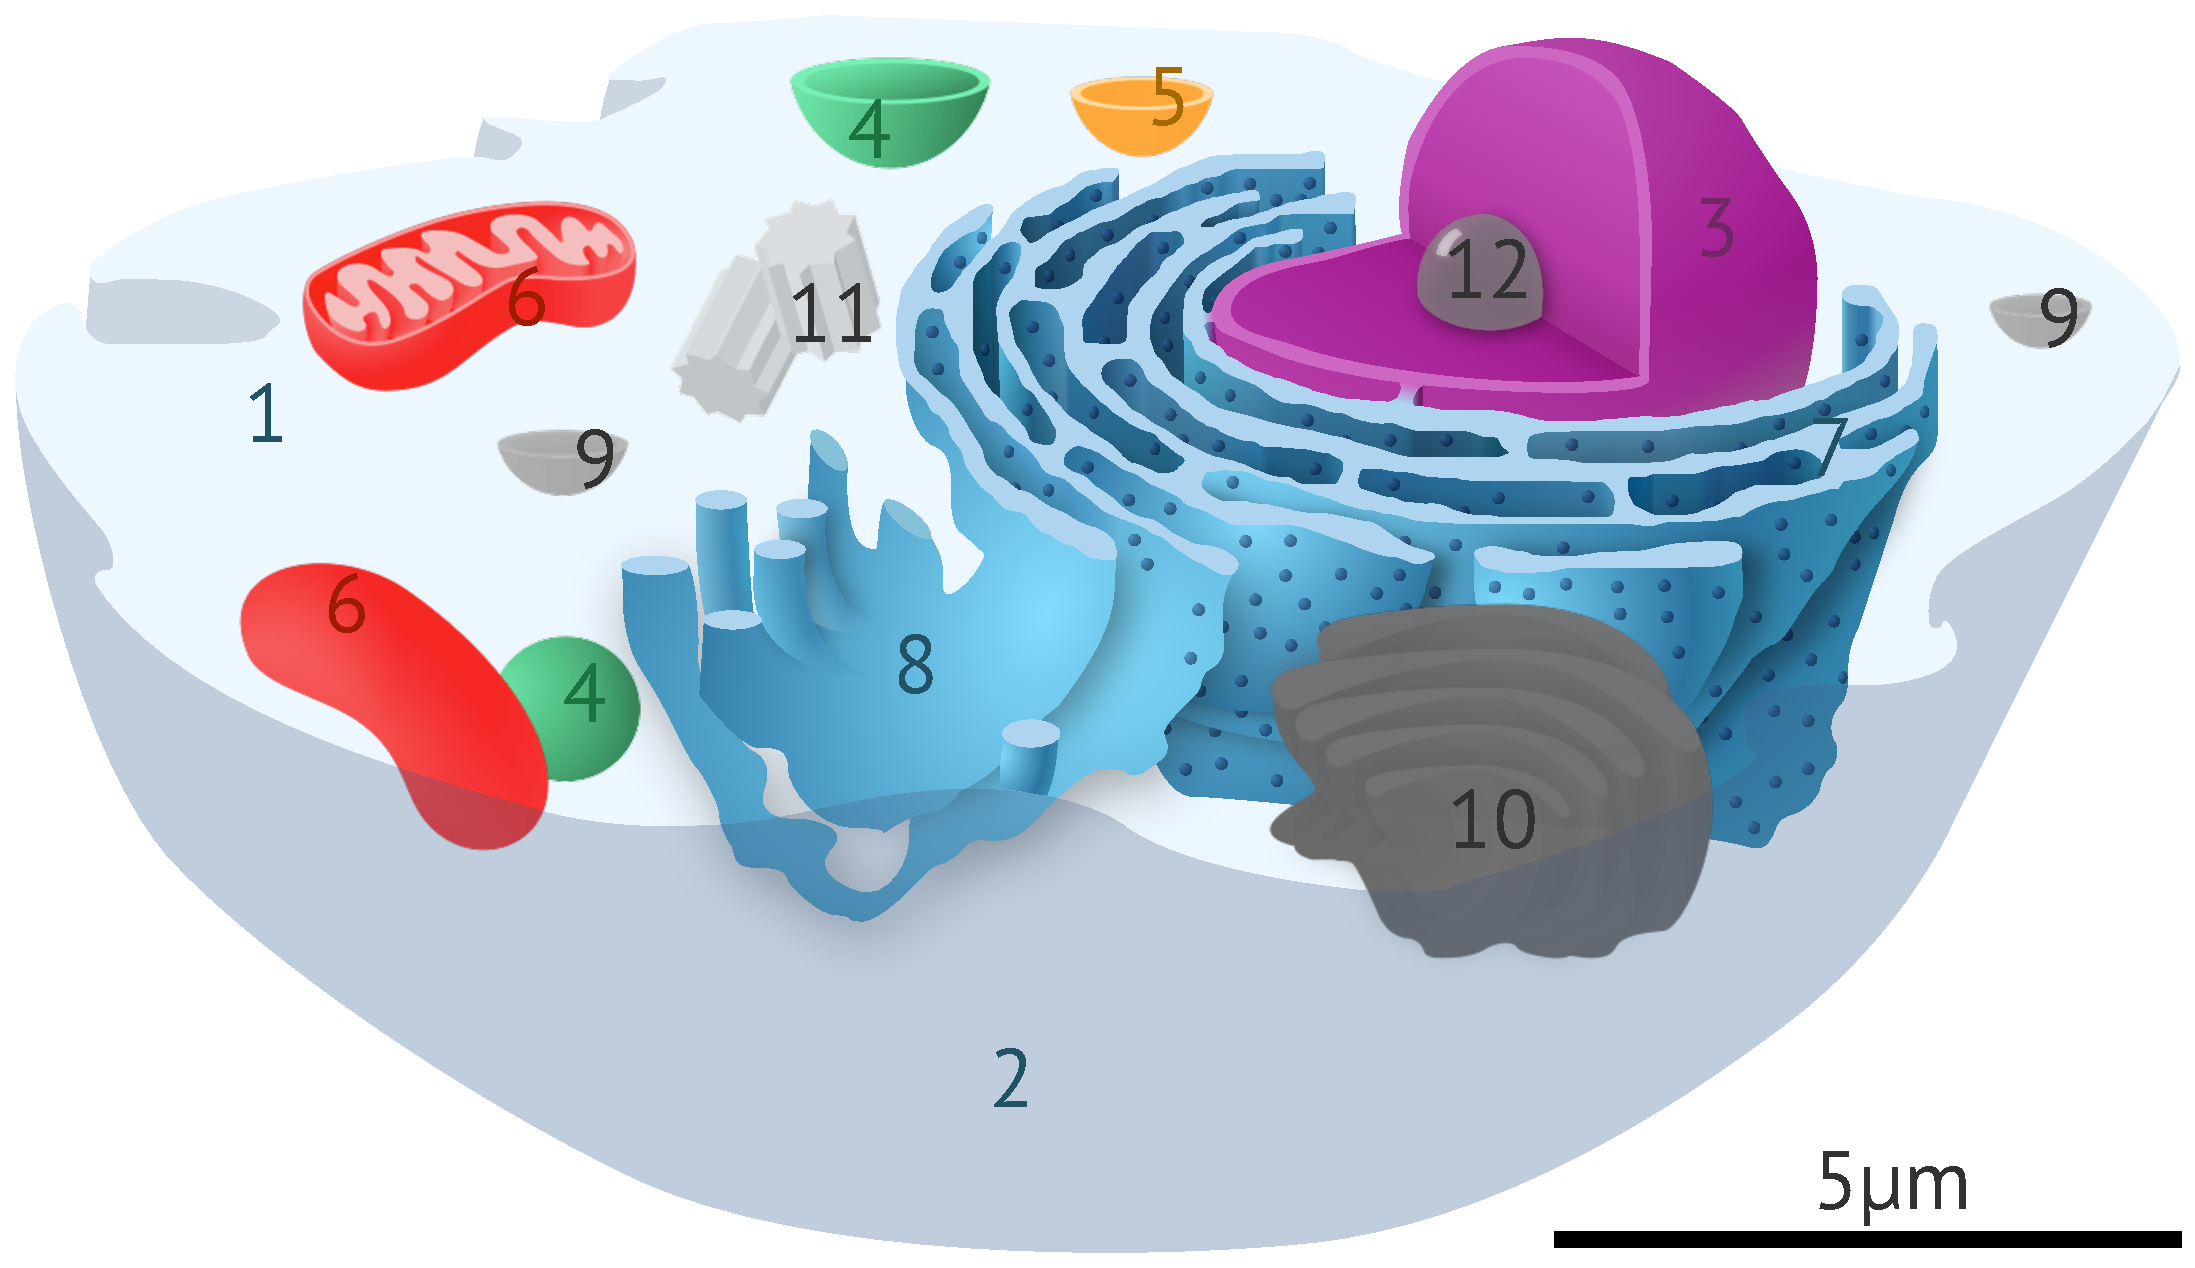
\includegraphics[width=1.0\textwidth]{animal-cell}
\captionsetup{singlelinecheck=off}
\caption[Introduction: Animal cell labelled with organelles relevant to this thesis]{A generic animal cell, adapted from Wikipedia~\cite{wikicell}, but with the organelles discussed in this thesis highlighted in colour. Numbered annotations are as follows:\newline
\begin{tabular}{p{0.3\textwidth}p{0.3\textwidth}p{0.3\textwidth}}
\begin{enumerate} 
	\item Cytosol 
	\item Cell membrane 
	\item Nucleus 
	\item Lysosome 
\end{enumerate} &
\begin{enumerate} \setcounter{enumi}{4}
	\item Endosome 
	\item Mitochondria 
	\item ER network 
	\item ER sheets 
\end{enumerate} &
\begin{enumerate} \setcounter{enumi}{8}
	\item Vesicle 
	\item Golgi apparatus 
	\item Centrosome 
	\item Nucleolus
\end{enumerate} \\
\end{tabular}} % end of caption!
\label{fig:animal-cell}
\end{figure}

Each of the organelles highlighted in Figure~\ref{fig:animal-cell} can be labelled with a fluorescent marker.
Fluorescent labelling can provide a variety of information about the cell, depending on the function of the organelles of interest~\cite{day2014fluorescent}. 

The cell nucleus contains DNA, the genetic encoding for life~\cite{alberts2002molecular}, and can be visualised under a microscope by labelling with DAPI or SiR-DNA~\cite{kapuscinski1995dapi, lukinavivcius2015sir}. 
Labelling the nucleus provides an easy method of automated cell counting, or an easy method for locating cells if it is not obvious from other labels~\cite{porter1980use}. 

The contents of the cell are contained by the cell membrane, which acts as a barrier between the contents of the cell and extra-cellular space~\cite{alberts2013essential}. 
Membrane proteins can be specifically labelled to visualise the outline of cells, to confirm whether another fluorescent object is located inside or outside the cell~\cite{yano2009tag, lee2011fluorescent, chamma2017optimized}. 

The cell can import useful raw materials into the cell through a process called endocytosis~\cite{alberts2002molecular}. 
To enter the cell, an intracellular compartment is created from the plasma membrane to contain the foreign material.
Once inside the cell, there are many pathways for processing the endocytosed contents~\cite{marsh2001endocytosis, marsh1999structural, mcmahon2011molecular}. 
A typical pathway delivers contents into small vesicles called early endosomes, which are selectively sorted to either recycle the contents to the cell membrane or develop into late endosomes. 
Late endosomes have an acidic environment, about pH\,\num{5.5}, and begin hydrolytic digestion of their contents~\cite{geisow1984ph}. 
Late endosomes mature into lysosomes with a more acidic environment and enzymes to further break down their contents~\cite{alberts2002molecular}. 
Labelling endosomes or lysosomes alongside other objects can be used for colocalisation studies, as performed in Chapter~\ref{chap:MOF}, which show whether another fluorescent substance is contained within the organelle or is free to move in the cytosol~\cite{pike2017quantifying}. 

\begin{figure}[htbp!]
\centering
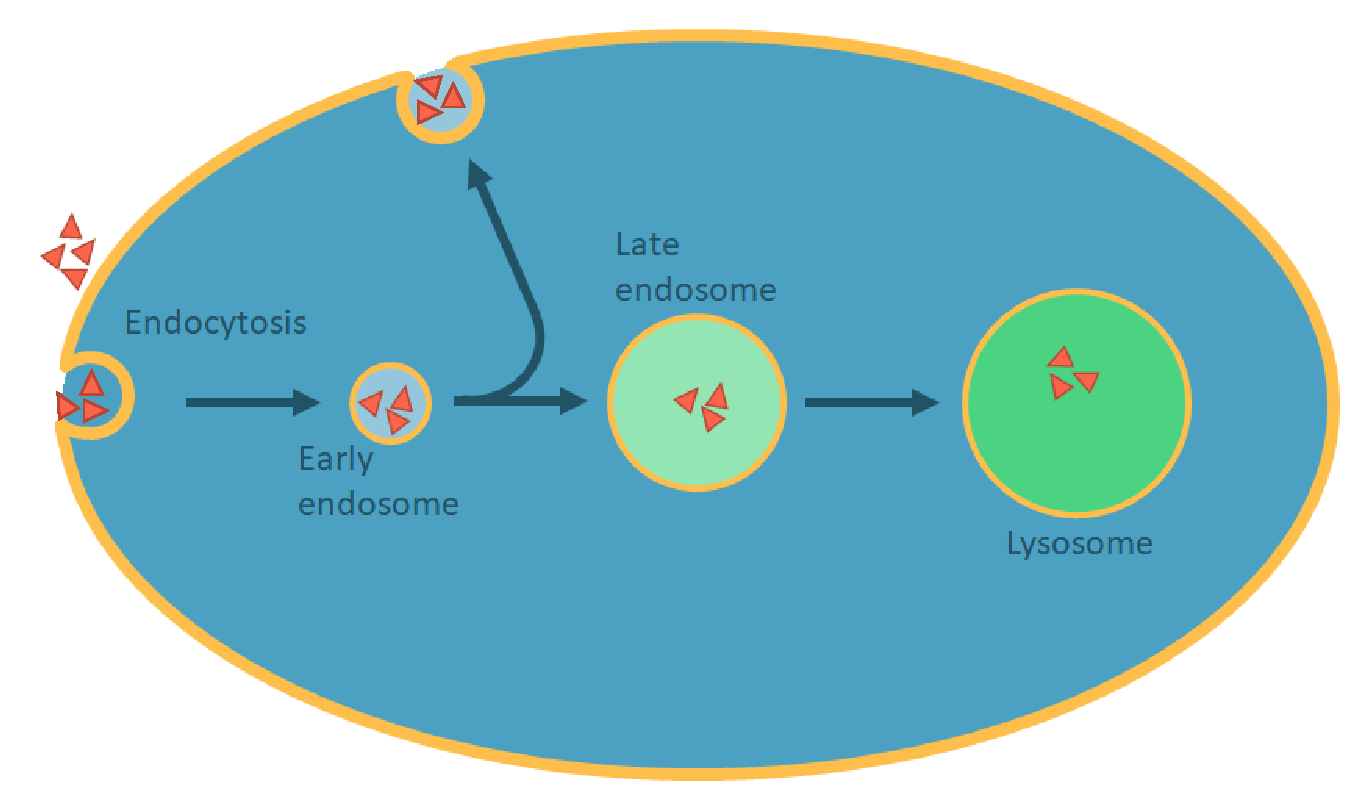
\includegraphics[width=1.0\textwidth]{endocytosis-pathway}
\captionsetup{singlelinecheck=off}
\caption[Introduction: Cells import external contents through endocytosis]{A typical endocytosis pathway, adapted from ~\cite{alberts2002molecular} shows the formation of various organelles, each of which contains a different environment for ingestion and processing of the external contents. Other endocytosis pathways also occur, for example to pass the contents to ER or release it directly into the cytosol. }
\label{fig:endocytosis-pathway}
\end{figure}

In addition to endosomes and lysosomes, other internal membrane structures include the endoplasmic reticulum (ER) and the Golgi apparatus. 
Protein folding and synthesis occurs in the ER; conversely, the Golgi apparatus is involved in further protein processing and secretion of substances from the cell~\cite{dyson1978cell}. 
Content is transferred between all intracellular compartments, either through vesicles or by direct organelle-organelle interaction. 
To visualise the ER, fluorescent labels can be applied to either the ER membrane or to luminal proteins contained within the ER network~\cite{costantini2013probing}; both labelling techniques are utilised in Chapter~\ref{chap:MOF}.  

Mitochondria generate energy for the cell by converting food to adenosine triphosphate (ATP), an energy-rich molecule that is used as the basic chemical fuel to power cellular activity~\cite{alberts2013essential}. 
This process, known as the Krebs cycle, consumes oxygen and produces carbon dioxide and water as waste products, so is a type of cellular respiration. 
Furthermore, mitochondria are responsible for triggering apoptosis - that is, controlled cell death~\cite{murray1993cell}. 
In cancer cells the Krebs cycle is bypassed, and ATP is produced by a more direct process known as glycolysis~\cite{warburg1930uber}. 
By avoiding the Krebs cycle, cancer cells stop the mitochondria from triggering apoptosis, such that the cells become immortal and reproduce to form tumours~\cite{murray1993cell}. 
Chapter~\ref{chap:MOF} uses fluorescently labelled  mitochondria to assess their interaction with a drug designed to restart the Krebs cycle in cancerous cells. 

All the organelles discussed in this sectiona are located in the cytosol, a crowded solution of many different types of molecules filling the volume of the cell~\cite{goodsell1991inside}. 
The solution is so dense that the cytosol behaves as a water-based gel rather than a liquid~\cite{alberts2013essential}. 

% Finally of relevance to this thesis is the cell's cytoskeleton. 

% Do I want to mention the cytoskeleton?? 

\section{Structure of this document}
Since October 2015, I have been working in the Laser Analytics Group building tools and applying them to answer biological questions. 

Chapter~\ref{chap:LAGSIM} describes the development of LAG SIM, a versatile, user-friendly structured illumination microscope. 
As well as the methods of hardware and software development, reconstruction theory is also discussed and a showcase of images is provided as a reference for capturing high-quality images. 

Chapter~\ref{chap:FPB} presents FPBioimage, an online tool for sharing and publishing 3D volumetric data. 
First developed for sharing reconstructed SIM data with a collaborator in Chicago, the chapter describes the development of the software, and presents a wide assortment of data from different 3D imaging technologies highlighting the unique features of the tool. 

Chapter~\ref{chap:MOF} demonstrates the capability of LAG SIM for facilitating hypothesis-driven research, introducing the use of metal organic frameworks as drug delivery vehicles for treating cancer. 
Three biological experiments are described showing various therapeutic effects offered by this newly developed technology. 

Chapter~\ref{chap:ER} utilises the fast, high-resolution imaging provided by LAG SIM to present pioneering discoveries about the endoplasmic reticulum. 
Computational analysis is used to understand and interpret experimental results, and compelling evidence is shown which advances the understanding of fundamental cell biology. 

Each chapter begins with its own detailed introduction to the topic, including background information and a review of relevant literature. 

Finally, a concluding Chapter~\ref{chap:conclusion} highlights the key discoveries and contributions made as part of this work.

\subsection{Aims of this document}
As a body of work, this document serves at least three purposes. 

Foremost, it is a document of evidence that I have designed and conducted my own research experiments, and have reached the level required for Doctor of Philosophy. 

Secondly, it is provided as a resource to researchers continuing my work in the Laser Analytics Group. 
Development and use of the tools is described in detail, which should allow for their continued development as new technology becomes available. 

Finally, this document provides a memento to myself of my PhD experience. 
I am proud of what I have achieved alongside my collaborators, and have included some of my favourite quotes at the start of each chapter; these simply serve as a reminder to myself that others appreciate my hard work and that the effort has undoubtedly been worth it. 


% Nomenclature command could be useful. 
%!TEX root = ../thesis.tex
%*******************************************************************************
%****************************** Second Chapter **********************************
%*******************************************************************************
\chapter{LAG SIM: A versatile, user-friendly structured illumination microscope} \label{chap:LAGSIM}

% Don't forget to PEE/L! 

% Note, figure labels are a bit of a mess here and need some fairly serious cleaning up! 04/10/18

% **************************** Define Graphics Path **************************
\ifpdf
    \graphicspath{{Chapter2/Figs/Raster/}{Chapter2/Figs/PDF/}{Chapter2/Figs/}}
\else
    \graphicspath{{Chapter2/Figs/Vector/}{Chapter2/Figs/}}
\fi

%``The LAG SIM works good now and I really love it!''
%
%\textit{Email from Meng Lu (Molecular Neuroscience Group, Cambridge), 26-06-2018}

\section{Introduction} \label{sec:simintro}
\subsection{Background to SIM} \label{sec:sim-background}
Widefield epifluorescent microscopes use a uniform field of light to illuminate a labelled sample~\cite[\textit{ch. 2}]{lakowicz2007principles}. 
Fluorescent emission light is then emitted from any fluorescent molecule located within the microscope's field of view~\cite{pawley2012handbook}. 
In this type of microscope, fluorescent molecules above and below the focal plane of the lens will also receive illumination light and fluoresce, causing an out-of-focus blur on the image~\cite{wilson1984theory}.

Out-of-focus light can be removed by placing a pinhole in the excitation and emission path, and scanning the small spot of light across the sample to build up an image one pixel at a time. 
This technique, invented in 1955 and called confocal microscopy, physically blocks out-of-focus light, making 3D reconstructions of samples possible~\cite{marvin1961microscopy}. 
The cost of this optical sectioning is a slow acquisition speed due to the nature of a point-scanning technique. 

A faster way of removing out-of-focus light can be achieved with total internal reflection fluorescence (TIRF)~\cite[\textit{ch. 21}]{periasamy2013methods}. 
In this scheme light is projected into the outer edge of the back-aperture of a specialised lens, such that it emerges from the lens steeper than the critical angle required for reflection, rather than refraction, from a glass interface. 
Although this means that no light passes through the microscope slide, as shown in Figure~\ref{fig:tirf-illumination}, energy from the evanescent field is able to couple into molecules close to the coverglass, inducing fluorescence~\cite{axelrod1981cell}. 
TIRF illuminates molecules within \SI{100}{\nano\metre} of the coverglass without obscuration by out-of-focus light, with the disadvantage that details deeper into the sample cannot be observed.

\begin{figure}[tbp]
\centering
\begin{subfigure}[b]{0.49\textwidth}
	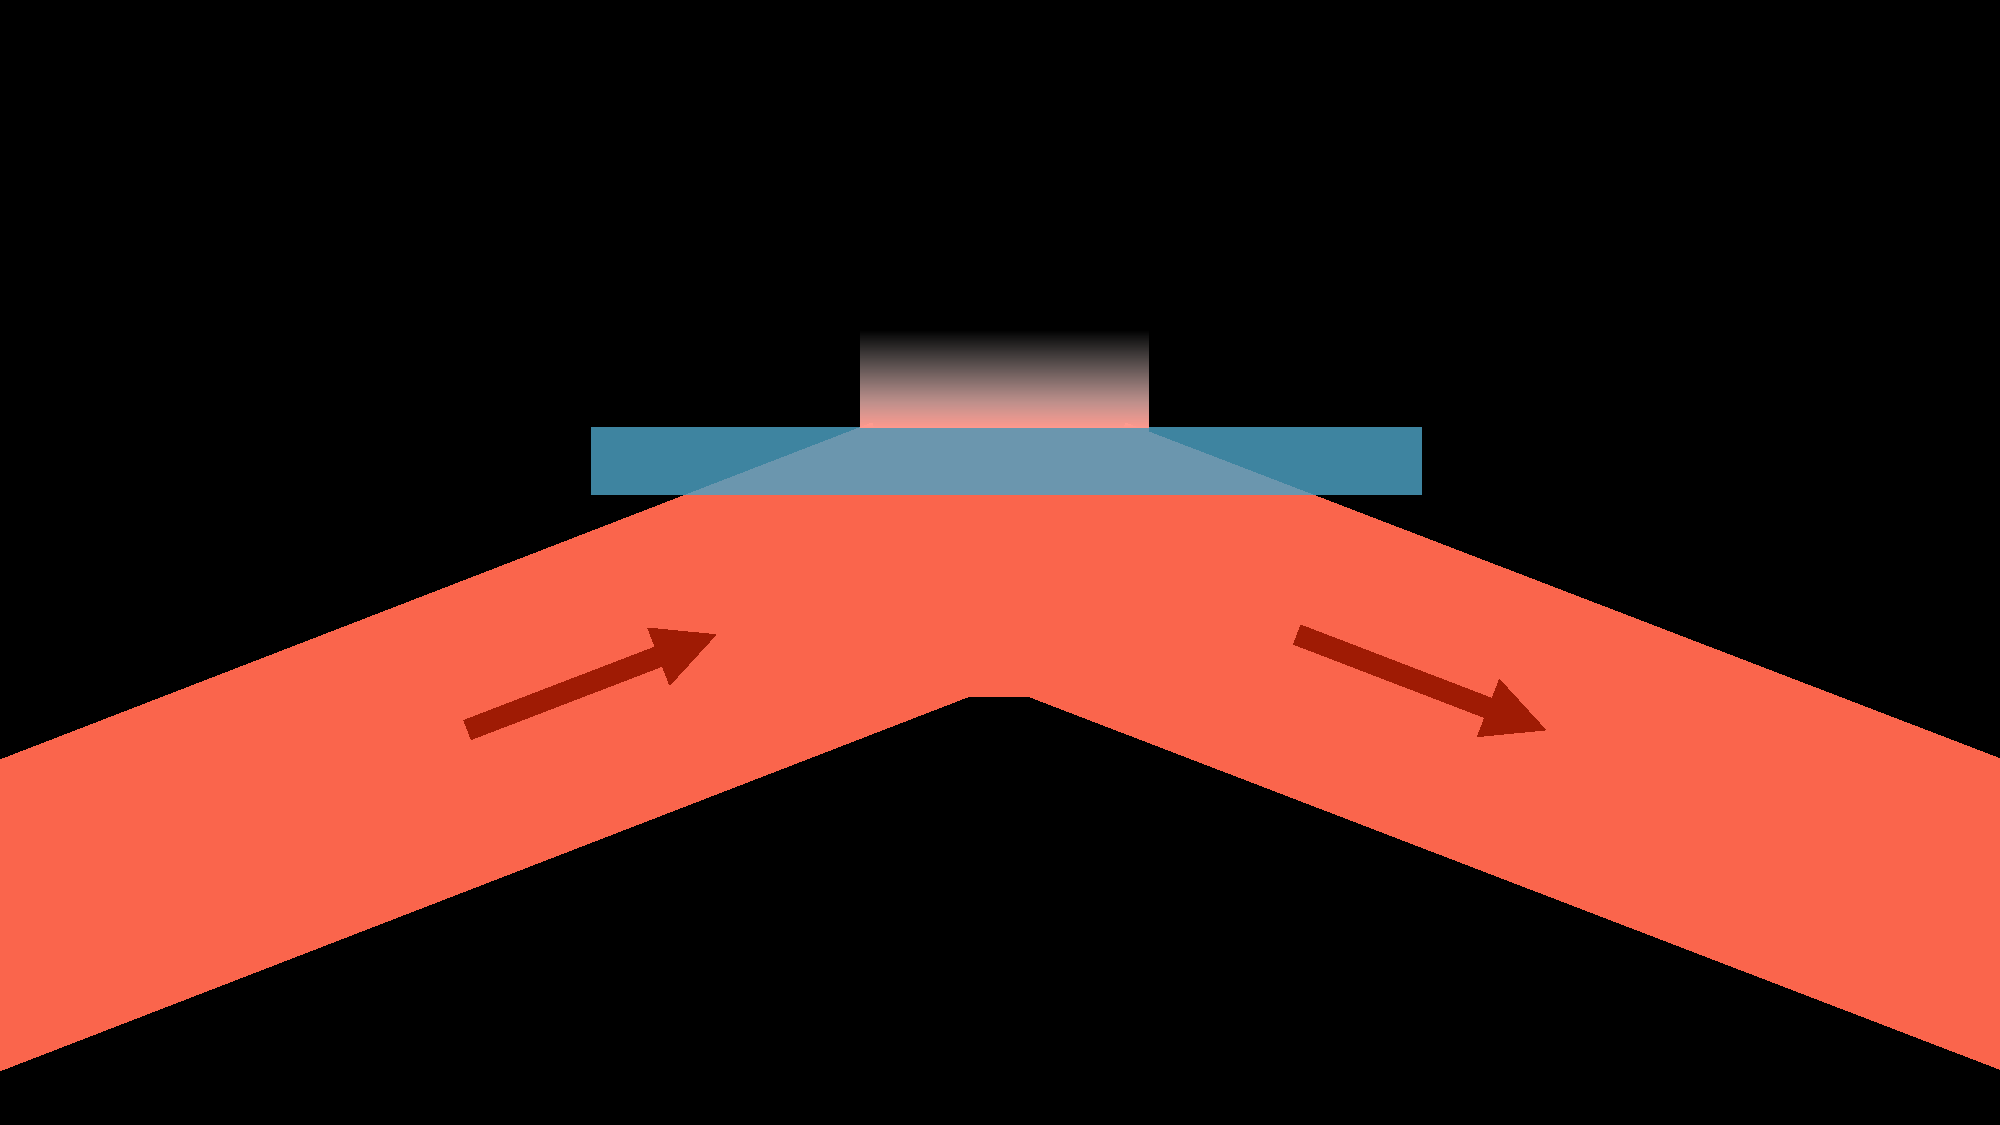
\includegraphics[width=\textwidth]{tirf-illumination}
	\caption{}\label{fig:tirf-illumination}
\end{subfigure}
\hfill
\begin{subfigure}[b]{0.49\textwidth}
	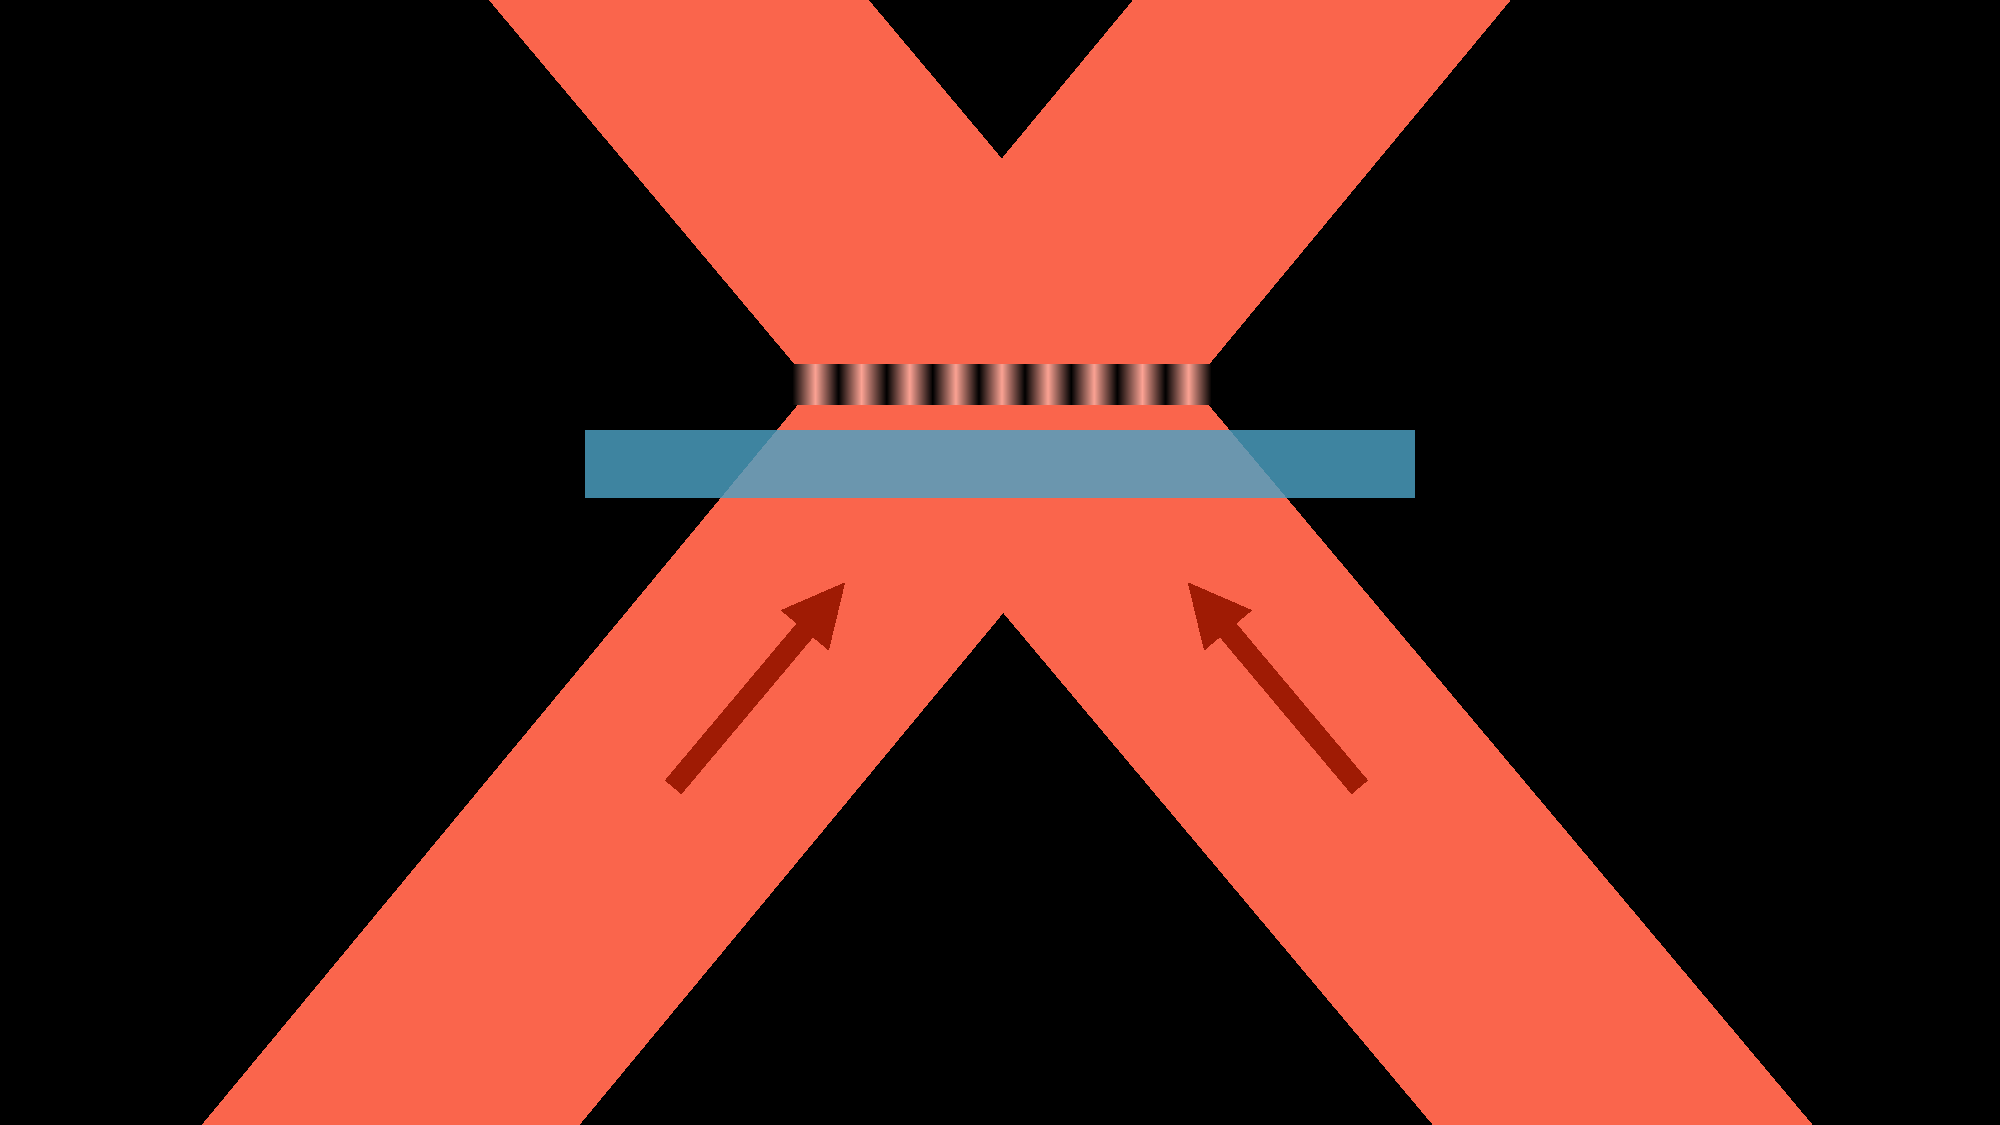
\includegraphics[width=\textwidth]{os-illumination}
	\caption{}\label{fig:os-illumination}
\end{subfigure}
\caption[LAG SIM: Both TIRF microscopy and structured illumination patterns can be used to remove out of focus light]{(a) shows a TIRF illumination scheme, where light intercepts the cover glass at an angle steeper than the critical angle for total internal reflection. The evanescent wave created can excite fluorphores in the closest \SI{100}{\nano\metre} to the coverglass, decaying exponentially in intensity. (b) shows the generation of a structured illumination pattern by the interference of two beams. This can be used to computationally reconstruct an optically sectioned image, as shown in Figure~\ref{fig:os-sim-comparison}. Diagrams are not to scale. }
\label{fig:os-sim-comparison}
\end{figure}

Sheppard and Wilson showed that optical sectioning can be achieved computationally if the illumination light is modulated with a structured pattern~\cite{pawley2012handbook, neil1997method}. 
Sinusoidal illumination can be produced by two coherent beams of light generated by a diffraction grating, which interfere at the focal plane of the objective lens as shown in Figure~\ref{fig:os-illumination}. 
The resulting image $I$ is described by Equation~\ref{eq:wilson-illumination}, where $W$ is the equivalent widefield image without structured illumination, $m$ the modulation depth, $t$ the modulation frequency, and $x$ a lateral spatial dimension in the sample plane.  

\begin{equation} \label{eq:wilson-illumination}
I_i = W \left( 1 + m \cos \left(t x + \phi_i \right) \right)
\end{equation}

Since the sinusoidal illumination pattern is only generated in the focal plane of the objective lens, extracting the $Wm$ component from Equation~\ref{eq:wilson-illumination} constructs an image $I_R$ in which the unmodulated out-of-focus light has been removed. 
Proofs~\ref{pro:square} and \ref{pro:homo} show that this requires the illumination to be stepped through three equally-spaced phases $\phi_i = \left\lbrace0, \frac{2\pi}{3}, \frac{4\pi}{3}\right\rbrace$, with an image $I_i$ captured at each step $i=\left\lbrace1,2,3\right\rbrace$. 
The proofs verify that either the square law detection of Equation~\ref{eq:wilson-square-law} or the homodyne detection shown in Equation~\ref{eq:wilson-homodyne} can be used to extract just the $Wm$ term~\cite{neil1997method}, multiplied in each case by a constant scaling factor. 

If the acquired images are simply summed together, the result $I_1+I_2+I_3$ is $W$, the image that would be obtained from a widefield microscope. 
Figure~\ref{fig:os-sim-widefield} shows this sum for an image of the herpes simplex virus infecting a human foreskin fibroblast (HFF) cell. 
When the raw images $I_i$ are reconstructed with the square-law detection of Equation~\ref{eq:wilson-square-law}, however, Figure~\ref{fig:os-sim} shows the effective removal of out-of-focus light. 

\begin{proof}
\caption{Square law detection removes out of focus light from 3 SIM images.}\label{pro:square}

\begin{equation*}
I_1 = W(1+m\cos(tx)),~I_2 = W(1+m\cos(tx+\frac{2\pi}{3})),~I_3 = W(1+m\cos(tx-\frac{2\pi}{3}))
\end{equation*}
\begin{equation*}
I_r^2 = (I_1 - I_2)^2 + (I_1 - I_3)^2 + (I_2 - I_3)^2
\end{equation*}
\textit{Substitute $I_1$, $I_2$, and $I_3$ into the expression for $I_r^2$:}

\begin{align*}
=W^2m^2\Bigg(\left(\cos(tx)-\cos(tx+\frac{2\pi}{3})\right)^2+&\left(\cos(tx)-\cos(tx-\frac{2\pi}{3})\right)^2\\&+\left(\cos(tx+\frac{2\pi}{3})-\cos(tx-\frac{2\pi}{3})\right)^2\Bigg)
\end{align*}

\textit{Expand squared brackets:}

\begin{align*}
=& W^2m^2\Big(2\cos^2(tx) + 2\cos^2(tx+\frac{2\pi}{3}) + 2\cos^2(tx-\frac{2\pi}{3}) 
 \\& - 2\cos(tx)\cos(tx+\frac{2\pi}{3}) - 2\cos(tx)\cos(tx-\frac{2\pi}{3}) - 2\cos(tx+\frac{2\pi}{3})\cos(tx-\frac{2\pi}{3})\Big)
\end{align*}

\textit{Apply double angle formulae to $\cos^2$ and $\cos(A)\cos(B)$ terms:}

\begin{align*}
= W^2m^2\Big(3 + \cos(2tx) &+ \cos(2tx+\frac{4\pi}{3}) + \cos(2tx-\frac{4\pi}{3})
- \cos(2tx+\frac{2\pi}{3}) \\&- \cos(-\frac{2\pi}{3}) - \cos(2tx-\frac{2\pi}{3}) - \cos(\frac{2\pi}{3}) -\cos(2tx) - cos(0)\Big)
\end{align*}

\textit{Note that $\cos(x+\phi) = \cos(x+2\pi n\phi)$, $n\in \mathbb{Z}$:}

\begin{align*}
= W^2m^2(3 + 0.5 + 0.5 - 1)
\end{align*}
\begin{align*}
= 3W^2m^2
\end{align*}

\textit{Take square root:}

\begin{align*}
I_r = \sqrt3Wm
\end{align*}

\end{proof}

\begin{proof}
\caption{Homodyne detection removes out of focus light from 3 SIM images. This gives the same result as square-law detection, albeit a different scaling factor. }\label{pro:homo}

\begin{equation*}
I_1 = W(1+m\cos(tx)),~I_2 = W(1+m\cos(tx+\frac{2\pi}{3})),~I_3 = W(1+m\cos(tx-\frac{2\pi}{3}))
\end{equation*}
\begin{equation*}
I_r = \abs{I_1 + I_2 \exp\left(\frac{2\pi j}{3}\right) + I_3 \exp\left(-\frac{2\pi j}{3}\right)}
\end{equation*}

\textit{Substitute $I_1$, $I_2$, and $I_3$ into the expression for $I_r$:}

\begin{align*}
= W &\abs{(1 + \exp\left(\frac{2\pi j}{3}\right) + \exp\left(-\frac{2\pi j}{3}\right)} \\
& + Wm \abs{\left(\cos(tx) + \cos(tx+\frac{2\pi}{3})(-0.5 + \frac{\sqrt3j}{2}) + \cos(tx-\frac{2\pi}{3})(-0.5 - \frac{\sqrt3j}{2}) \right)}
\end{align*}

\textit{Note that $\abs{(1 + \exp\left(\frac{2\pi j}{3}\right) + \exp\left(-\frac{2\pi j}{3}\right)}=0$:}

\begin{align*}
= Wm \abs{\left(\cos(tx) + \cos(tx+\frac{2\pi}{3})(-0.5 + \frac{\sqrt3j}{2}) + \cos(tx-\frac{2\pi}{3})(-0.5 - \frac{\sqrt3j}{2}) \right)}
\end{align*}

\textit{Gather real and imaginary terms:}

\begin{align*}
= Wm \Bigg\lvert\cos(tx) - &0.5\left(\cos(tx+\frac{2\pi}{3})+(\cos(tx-\frac{2\pi}{3})\right) \\ &+ \frac{\sqrt3j}{2}\left(\cos(tx+\frac{2\pi}{3})-(\cos(tx-\frac{2\pi}{3})\right)\Bigg\rvert
\end{align*}

\textit{Apply double angle formulae for $2\cos(A)\cos(B)$ and $2\sin(A)\sin(B)$:}

\begin{equation*}
= Wm \abs{\cos(tx) - \left(\cos(tx)\cos(\frac{2\pi}{3})\right) + \sqrt3j\left(\cos(tx)\cos(\frac{2\pi}{3})\right)}
\end{equation*}
\begin{equation*}
= Wm \abs{\cos(tx) + 0.5\cos(tx) - \frac{3j}{2}\sin(tx)}
\end{equation*}
\begin{equation*}
= \frac{3}{2}Wm \abs{\cos(tx)-j\sin(tx)}
\end{equation*}
\begin{equation*}
I_r = \frac{3}{2}Wm
\end{equation*}
\end{proof}

\begin{figure}[tb]
\centering
\begin{subfigure}[b]{0.49\textwidth}
	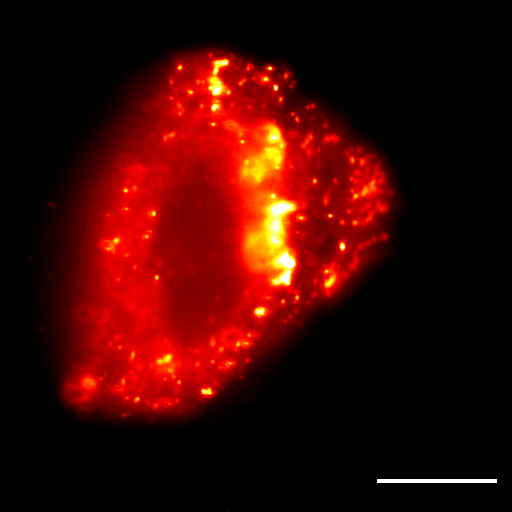
\includegraphics[width=\textwidth]{os-sim-widefield}
	\caption{}\label{fig:os-sim-widefield}
\end{subfigure}
\hfill
\begin{subfigure}[b]{0.49\textwidth}
	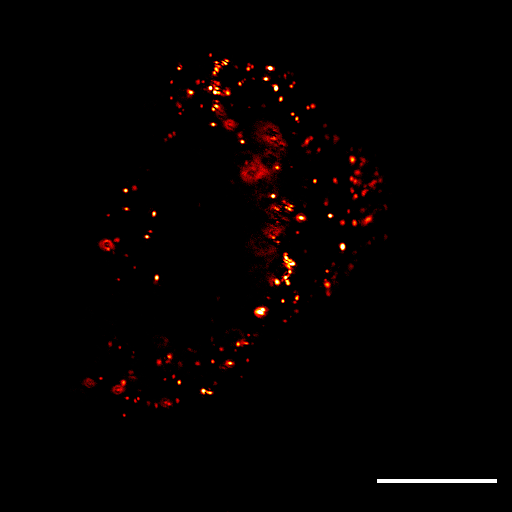
\includegraphics[width=\textwidth]{os-simd}
	\caption{}\label{fig:os-sim}
\end{subfigure}
\caption[LAG SIM: Structured illumination can be used to computationally remove out of focus light]{(a) shows a widefield image, $W$, of herpes virus infecting a human foreskin fibroblast (HFF) cell. (b) shows the same image after illumination with 3 phase-stepped sinusoidal patterns, which are only generated at the focal plane of the objective lens. Combining the images with square-law detection shown in Equation~\ref{eq:wilson-square-law} leaves just the $Wm$ term derived in Proofs~\ref{pro:square} and \ref{pro:homo}, effectively removing the out-of-focus light. Human foreskin fibroblast (HFF) cells were prepared and infected by Katharina Scherer. Scalebar is \SI{10}{\micro\metre}. } 
\label{fig:os-sim-comparison}
\end{figure}

\begin{equation} \label{eq:wilson-square-law}
I_R = \left( \left( I_1 - I_2 \right)^2 + \left( I_2 - I_3 \right)^2 + \left( I_1 - I_3 \right)^2 \right)^{\frac{1}{2}} = \sqrt{3}Wm
\end{equation}

\begin{equation} \label{eq:wilson-homodyne}
I_R = \abs{ I_1 + I_2 \exp\left(\frac{2\pi j}{3} \right) + I_3 \exp\left(\frac{4\pi j}{3}\right) } = \frac{3}{2}Wm
\end{equation}
~\newline

The result of Proofs~\ref{pro:square} and \ref{pro:homo} show that the signal in the reconstructed image is directly proportional to the modulation depth $m$ of the sinusoidal illumination pattern. 
Since the noise power is constant with respect to modulation depth, the signal-to-noise ratio of the reconstructed image is also directly proportional to the modulation depth. 
It is therefore important to maximise the modulation depth to reconstruct an optically-sectioned image with as high a signal-to-noise ratio as possible.

\subsection{SIM for resolution doubling} \label{sec:SIM-theory}
The widefield image $W$ produced by a fluorescent microscope is made up of the underlying sample fluorescence, $S$, convolved with the microscope point spread function (PSF), $H$. 
When light from the sample plane passes through a lens, the finite aperture means that a small point of light is spread into a larger spot in the image plane~\cite[\textit{ch. 11}]{hecht2017optics}. 
This means that two independent points of light which are too close together cannot be resolved; that is, the lens acts as a low pass filter for spatial frequencies. 
This can be seen in the diffraction-limited image of \SI{100}{\nano\metre} beads in Figure~\ref{fig:beads-widefield}, where the beads' fluorescence emission light spreads into a spot with a full-width half-maximum (FWHM) of \SI{200}{\nano\metre}. 
The corresponding Fourier-space image in Figure~\ref{fig:fourier-widefield} shows that spatial frequencies above the diffraction limit are not transmitted through the lens. 

\begin{figure}[p]
\centering
\begin{subfigure}[b]{0.45\textwidth}
	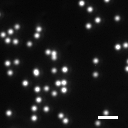
\includegraphics[width=\textwidth]{r01}
	\caption{}\label{fig:beads-widefield}
\end{subfigure}
\raisebox{9.3em}{\noindent\Huge$\Leftrightarrow$}
\begin{subfigure}[b]{0.45\textwidth}
	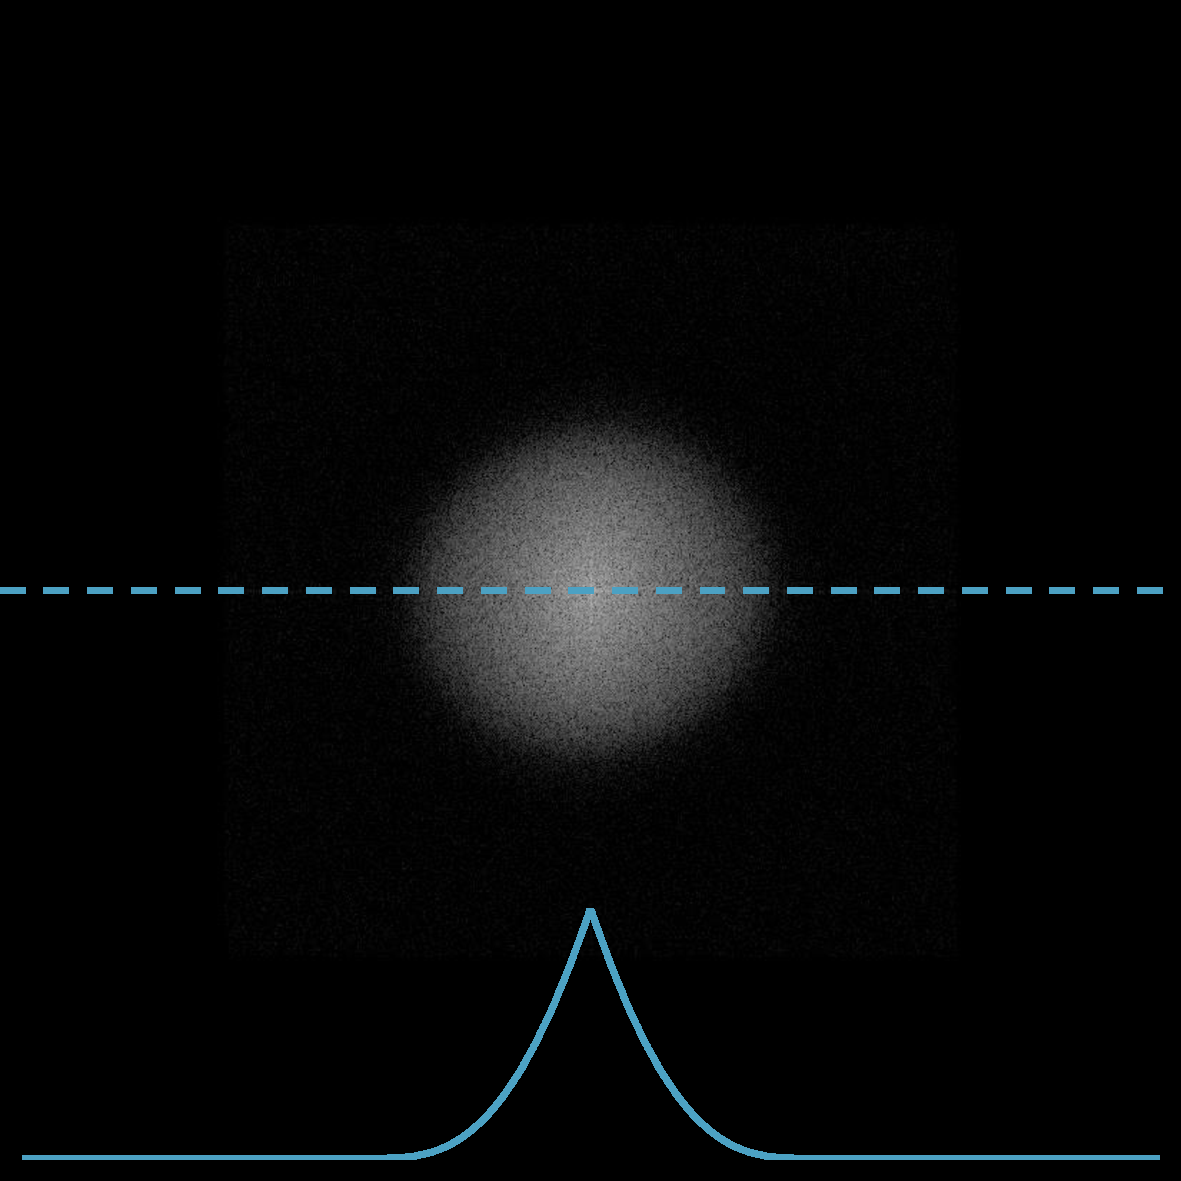
\includegraphics[width=\textwidth]{f01}
	\caption{}\label{fig:fourier-widefield}
\end{subfigure}
~\newline
\begin{subfigure}[b]{0.45\textwidth}
	
\includegraphics[width=\textwidth]{r02}
	\caption{}\label{fig:beads-raw-SIM}
\end{subfigure}
\raisebox{9.3em}{\noindent\Huge$\Leftrightarrow$}
\begin{subfigure}[b]{0.45\textwidth}
	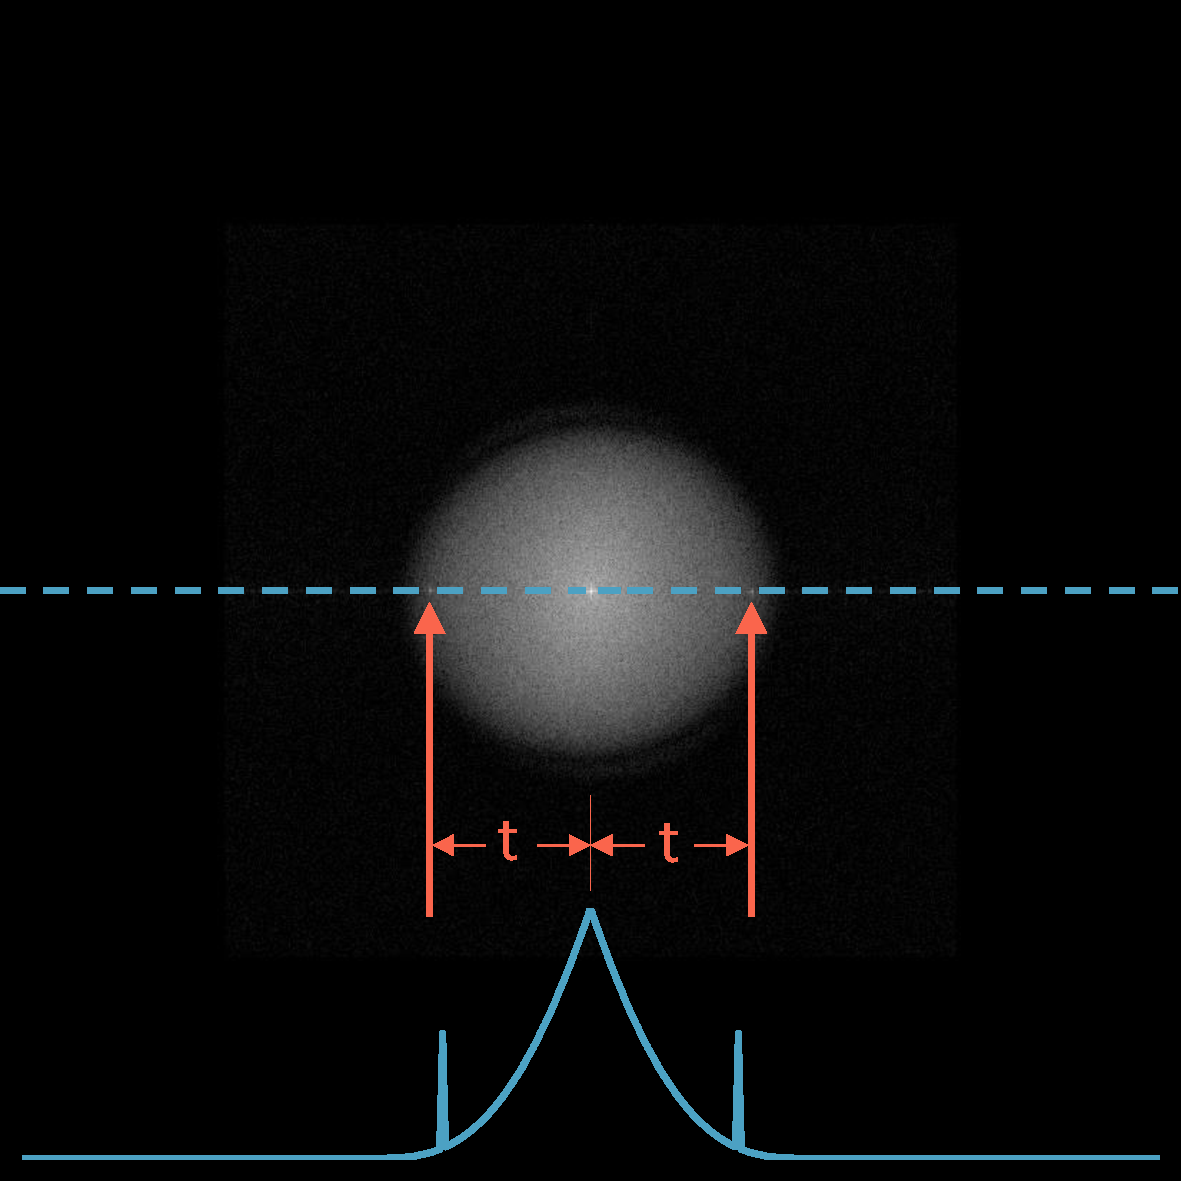
\includegraphics[width=\textwidth]{f02}
	\caption{}\label{fig:fourier-raw-SIM}
\end{subfigure}
~\newline
\begin{subfigure}[b]{0.45\textwidth}
	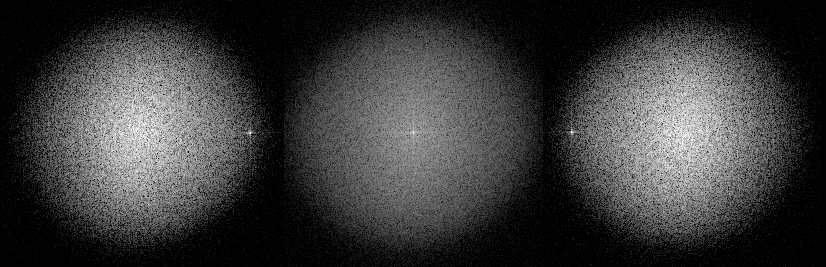
\includegraphics[width=\textwidth]{fourier-components}
	\caption{}\label{fig:fourier-components}
\end{subfigure}
\caption[LAG SIM: A sinusoidal illumination pattern is visible as delta peaks in Fourier space]{(a) shows a diffraction-limited image of \SI{100}{\nano\metre} beads. 
(b) shows that spatial frequencies above the diffraction limit of the lens are not transmitted, causing a point-spread function which increases the apparent size of the beads and preventing two beads which are close together from being resolved. 
(c) shows the same field of view under structured illumination; note that some beads are less intense than in (a) if they fall within a trough of the sinusoidal illumination pattern. 
(d) clearly shows delta peaks appearing in the Fourier transform of (c) due to the sinusoidal illumination, at a distance from the origin equal to the spatial frequency of the illumination pattern. 
(e) shows the Fourier components $\hat{H}\hat{S}\left(k_x\right)$, $\hat{H}\hat{S}\left(k_x+t\right)$, and $\hat{H}\hat{S}\left(k_x-t\right)$ extracted from the raw images by Equation~\ref{eq:matrix-inversion}. Scalebars are \SI{1}{\micro\metre}.
}
\label{fig:fourier-reconstruction}
\end{figure}

\begin{figure}[p]
\centering
\begin{subfigure}[b]{0.45\textwidth}
	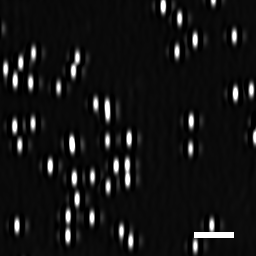
\includegraphics[width=\textwidth]{r04}
	\caption{}\label{fig:beads-x-doubling}
\end{subfigure}
\raisebox{9.3em}{\noindent\Huge$\Leftrightarrow$}
\begin{subfigure}[b]{0.45\textwidth}
	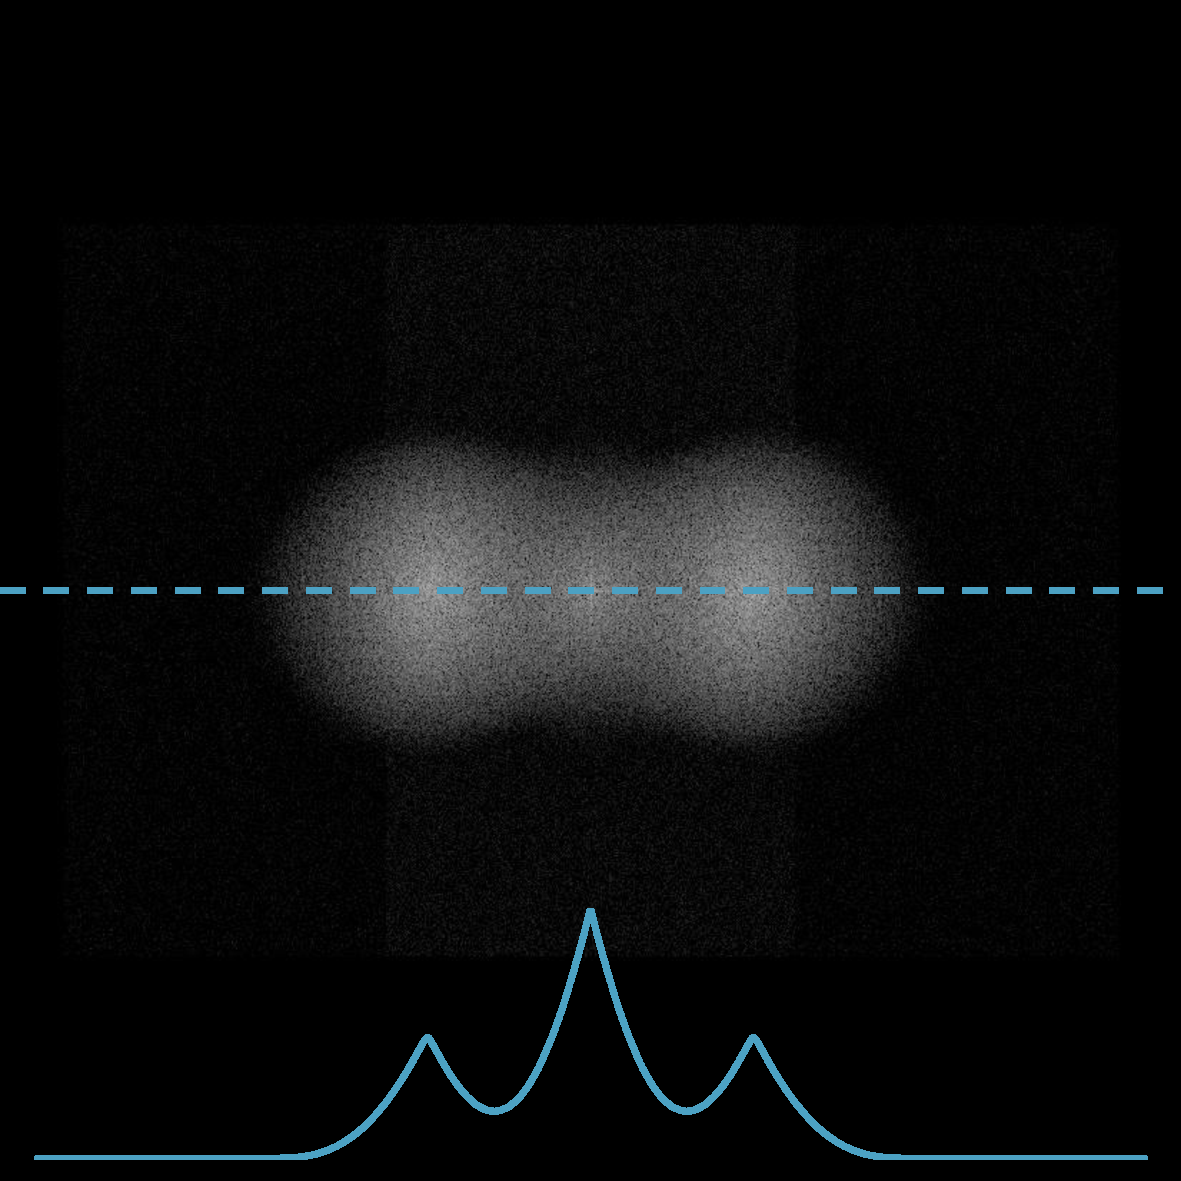
\includegraphics[width=\textwidth]{f04}
	\caption{}\label{fig:fourier-x-doubling}
\end{subfigure}
~\newline
\begin{subfigure}[b]{0.45\textwidth}
	
\includegraphics[width=\textwidth]{r05}
	\caption{}\label{fig:beads-isotropic-doubling}
\end{subfigure}
\raisebox{9.3em}{\noindent\Huge$\Leftrightarrow$}
\begin{subfigure}[b]{0.45\textwidth}
	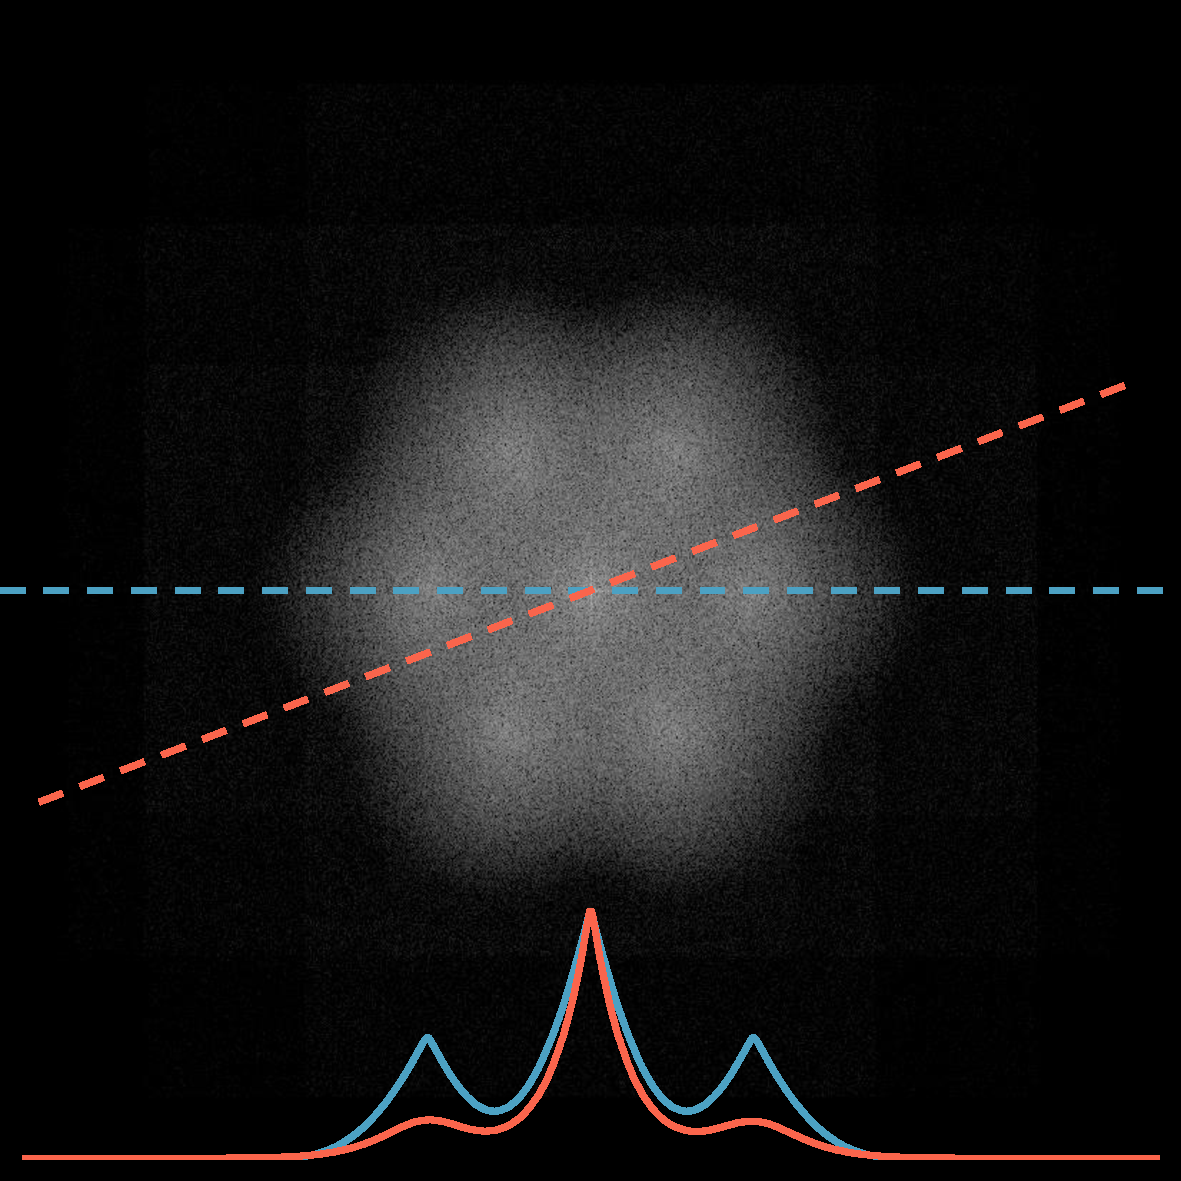
\includegraphics[width=\textwidth]{f05}
	\caption{}\label{fig:fourier-isotropic-doubling}
\end{subfigure}
\caption[LAG SIM: Reconstruction of SIM images takes place in Fourier space]{(a) shows beads after SIM reconstruction in the x-direction only, where the increase in x-resolution makes the circular beads appear as elongated ellipses.  (b) shows the corresponding Fourier-space image, where the width of the support confirms that resolution has doubled in the x-direction compared to widefield. (c) shows an isotropic increase in resolution, achieved by performing the procedure used to generate (a) at two more angles, \SI{60}{\degree} and \SI{120}{\degree} to the x-axis. (d) shows the Fourier transform of (c), confirming isotropic resolution increase. Notably, this reconstruction scheme produces peaks of signal in Fourier space and the OTF is not rotationally symmetric, causing the characteristic hexagonal artefacts visible in (c). Scalebars are \SI{1}{\micro\metre}.}
\label{fig:fourier-reconstruction}
\end{figure}

The same structured illumination microscopy (SIM) used for optical sectioning can be re-purposed for surpassing the diffraction limit. 
First discussed by Lucosz~\cite{lukosz1966optical}, and then more explicitly described by Heintzmann for sinusoidal illumination patterns~\cite{heintzmann1999laterally}, the first experimental result showing 2D isotropic resolution doubling with 9 raw image acquisitions was published by Gustafsson in the year \num{2000}~\cite{gustafsson2000surpassing}. 
Heintzmann shows that if we take the Fourier transform of the acquired images shown in Equation~\ref{eq:wilson-illumination}, we obtain the set of images shown in Equation~\ref{eq:heintzmann-fourier}; where \^{}-symbols represent 2D Fourier transforms of their equivalent variables, and $k_x$ is the Fourier variable of $x$, that is $f(x) \Leftrightarrow \hat{f}(k_x)$. 
Note that $W$ has been replaced with its underlying components $H\otimes S \Leftrightarrow \hat{H}\hat{S}$, where $\hat{H}$, the Fourier transform of the PSF, is known as the optical transfer function (OTF). 

\begin{equation} \label{eq:heintzmann-fourier}
\hat{I_i} = \hat{H} \hat{S} \otimes \left( \delta \left( k_x \right) + \frac{m}{2} e^{j\phi_i} \delta \left( k_x + t \right) + \frac{m}{2} e^{-j\phi_i} \delta \left( k_x - t \right) \right) 
\end{equation}

Each acquired raw image contains contributions from each of 3 shifted Fourier components. 
Using $\phi_i = \left\lbrace0, \frac{2\pi}{3}, \frac{4\pi}{3}\right\rbrace$, these Fourier components can be separated into individual images by solving the set of simultaneous equations for $\hat{S}\otimes\delta \left( k_x \right)$, $\hat{S}\otimes\delta \left( k_x + t \right)$, and $\hat{S}\otimes\delta \left( k_x - t \right)$ with matrix inversion, as shown in Figure~\ref{fig:fourier-components} and Equation~\ref{eq:matrix-inversion}~\cite{wicker2013phase}. 
Assuming phase steps are all equal, performing a 3D Fourier transform of the phase-stepped raw images stacked in the 3rd dimension produces the same result~\cite{gustafsson2005nonlinear}. 

\begin{equation} \label{eq:matrix-inversion}
\begin{bmatrix} \hat{H}\hat{S}\left(k_x\right) \\ \hat{H}\hat{S}\left(k_x+t\right) \\ \hat{H}\hat{S}\left(k_x-t\right) \end{bmatrix} = 
\begin{bmatrix}
1 & \frac{m}{2}\exp\left(0j\right) & \frac{m}{2}\exp\left(-0j\right) \\ 
1 & \frac{m}{2}\exp\left(\frac{2\pi j}{3}\right) & \frac{m}{2}\exp\left(-\frac{2\pi j}{3}\right) \\ 
1 & \frac{m}{2}\exp\left(\frac{4\pi j}{3}\right) & \frac{m}{2}\exp\left(-\frac{4\pi j}{3}\right)
\end{bmatrix}^{-1}
\begin{bmatrix} \hat{I_1} \\ \hat{I_2} \\ \hat{I_3} \end{bmatrix}
\end{equation}

When the matrix of Equation~\ref{eq:matrix-inversion} is inverted, an factor of $m$ can be extracted as a scaling factor in front of the high frequency Fourier components, shown in Equation~\ref{eq:matrix-solved}. 
In the same way that a smaller modulation depth $m$ reduces the signal-to-noise ratio in optical sectioning SIM, described in Section~\ref{sec:sim-background}, this factor shows that the signal-to-noise ratio of the high frequency components is directly proportional to the modulation depth of the illumination pattern. 

\begin{equation} \label{eq:matrix-solved}
\begin{bmatrix} \hat{H}\hat{S}\left(k_x\right) \\ m\hat{H}\hat{S}\left(k_x+t\right) \\ m\hat{H}\hat{S}\left(k_x-t\right) \end{bmatrix} = 
\frac{1}{3} \begin{bmatrix}
1 & 1 & 1 \\ 
2 & \left(-1 -\sqrt{3}j\right) & \left(-1+\sqrt{3}j\right) \\ 
2 & \left(-1 +\sqrt{3}j\right) & \left(-1 -\sqrt{3}j\right)
\end{bmatrix}
\begin{bmatrix} \hat{I_1} \\ \hat{I_2} \\ \hat{I_3} \end{bmatrix}
\end{equation}

To complete the reconstruction, the separated Fourier components must be placed at the correct position in Fourier space, as determined by $t$. 
Assuming the sinusoidal illumination pattern is generated by the same lens used for imaging the sample, the highest frequency sinusoid which can be generated will correspond to delta peaks at the edge of the microscope's support in Fourier space~\cite{heintzmann2017super}, visible in Figure~\ref{fig:fourier-raw-SIM}. 
When the components are shifted into the appropriate location, the support of the OTF doubles in the $x$ direction, as shown in Figure~\ref{fig:fourier-x-doubling}. 
Figure~\ref{fig:beads-x-doubling} confirms that resolution is doubled in the x-direction, which makes the circular beads appear as elongated ellipses. 

To achieve isotropic 2D resolution doubling, the sinusoidal illumination pattern must be rotated to cover more area in Fourier space. 
Typically a total of three rotations are used, at \SI{60}{\degree} and \SI{120}{\degree} to the original pattern orientation~\cite{gustafsson2000surpassing, chang2009isotropic}. 
Performing the reconstruction procedure on all 9 images produces the Fourier space reconstruction shown in Figure~\ref{fig:fourier-isotropic-doubling}, showing an isotropic increase in the resolution support. 
% Support is the closure of the set of points at which the Fourier transform takes a non-zero value


The final step for this reconstruction procedure is to inverse Fourier transform the reconstructed Fourier space image of Figure~\ref{fig:fourier-isotropic-doubling} to produce Figure~\ref{fig:beads-isotropic-doubling}, an image with double the equivalent widefield resolution. 
Comparing Figure~\ref{fig:beads-isotropic-doubling} to Figure~\ref{fig:beads-widefield}, the beads appear smaller and two close beads which could not be resolved before can now be distinguished. 
However, the reconstruction procedure must be refined to reduce the hexagonal artefacts introduced by this reconstruction method. 

\subsection{Refining the reconstruction algorithm reduces artefacts}
The 2D OTF of a focussed lens is a rotationally symmetric function which gradually reduces to zero as spatial frequency increases~\cite{williams2002introduction}. 
The line profile through the OTF of an ideal lens in Figure~\ref{fig:fourier-widefield} shows that the higher the spatial frequency, the less contrast the microscope produces.
In a practical set-up, noise further limits the resolvable contrast at high frequencies, such that signal-to-noise ratio decreases as spatial frequency increases. 

\begin{figure}[tbp]
\vspace{-6pt} \centering
\begin{subfigure}[b]{0.45\textwidth}
	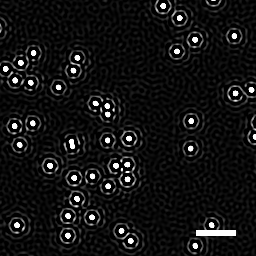
\includegraphics[width=\textwidth]{r06}
	\caption{}\label{fig:beads-wiener}
\end{subfigure}
\raisebox{9.3em}{\noindent\Huge$\Leftrightarrow$}
\begin{subfigure}[b]{0.45\textwidth}
	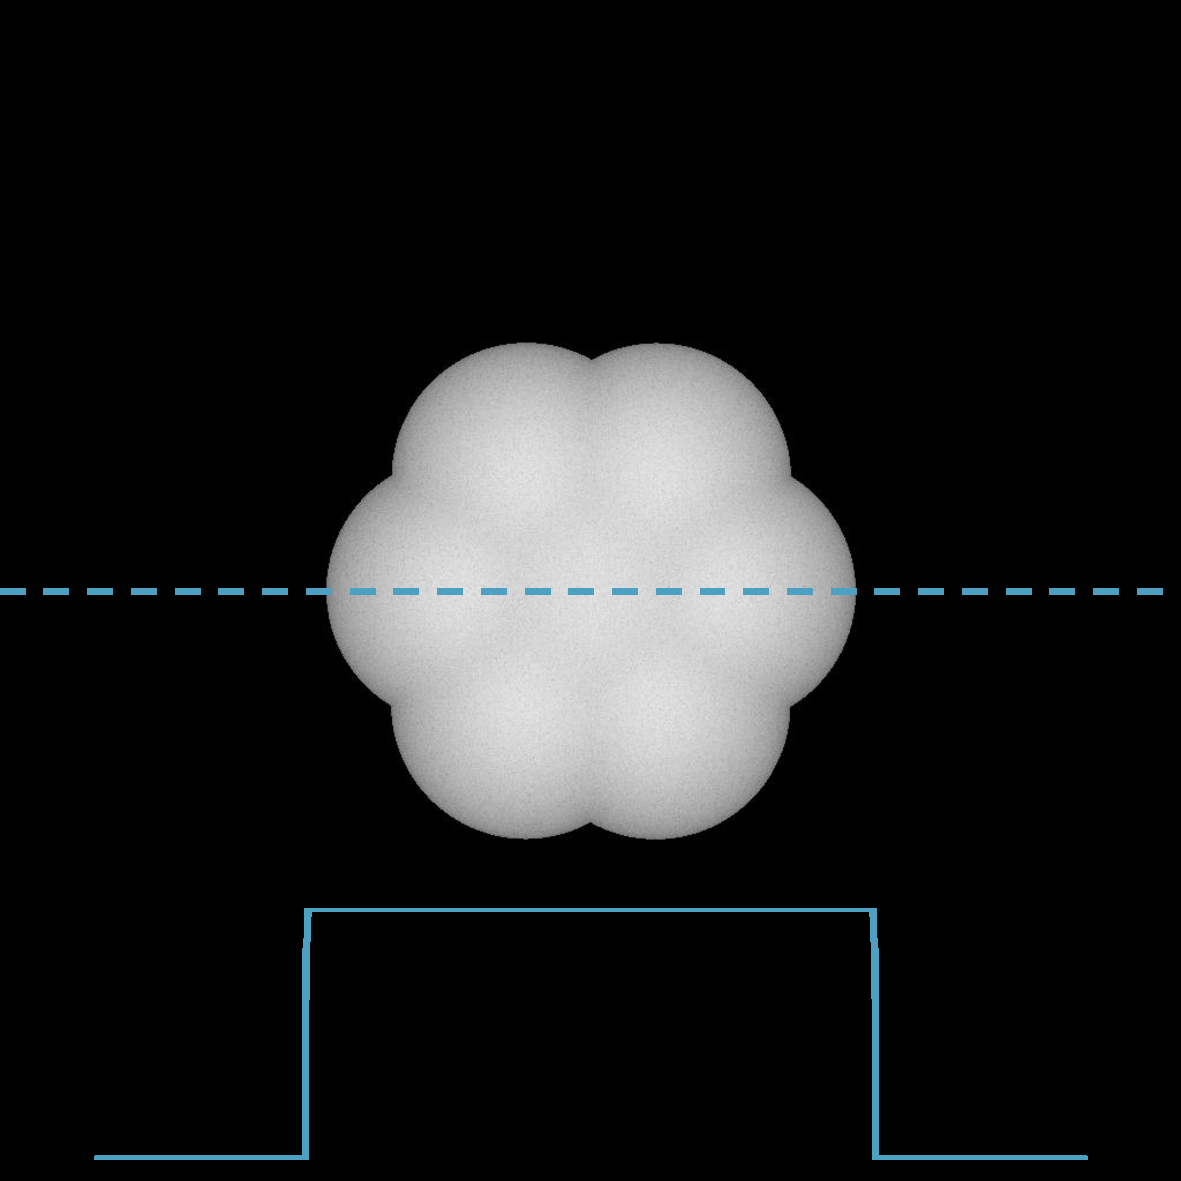
\includegraphics[width=\textwidth]{f06}
	\caption{}\label{fig:fourier-wiener}
\end{subfigure}

~\newline
\begin{subfigure}[b]{0.45\textwidth}
	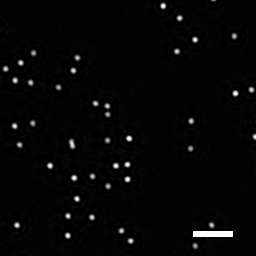
\includegraphics[width=\textwidth]{r07}
	\caption{}\label{fig:beads-apodised}
\end{subfigure}
\raisebox{9.3em}{\noindent\Huge$\Leftrightarrow$}
\begin{subfigure}[b]{0.45\textwidth}
	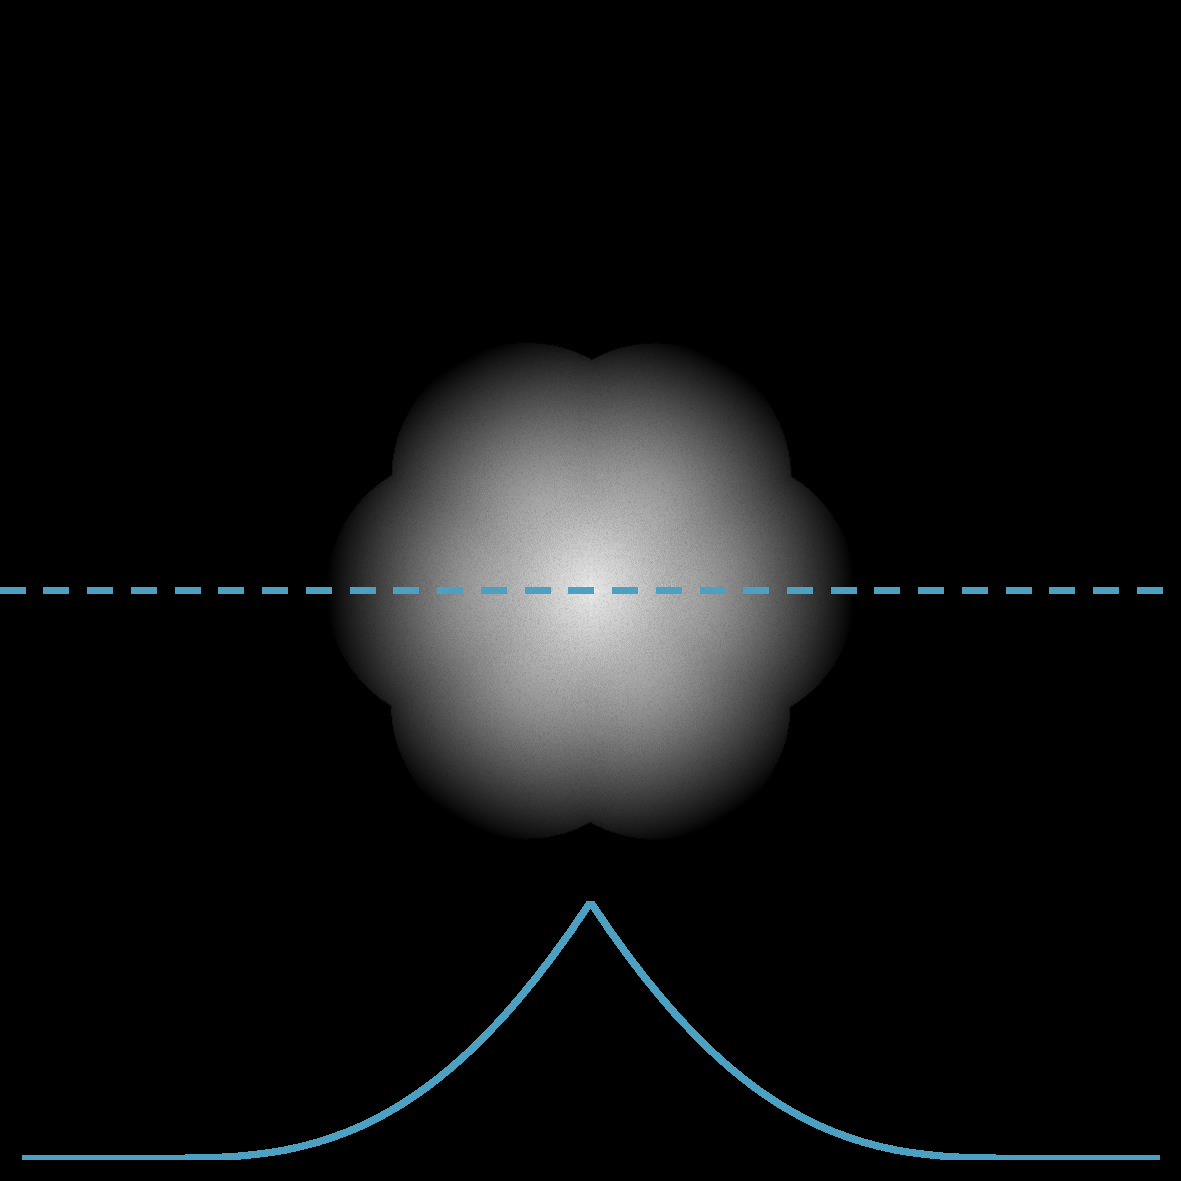
\includegraphics[width=\textwidth]{f07}
	\caption{}\label{fig:fourier-apodised}
\end{subfigure}
\caption[LAG SIM: Wiener filtering of the SIM OTF is required for artefact-free reconstruction]{(a) shows a reconstructed SIM image after Wiener filtering described in Equation~\ref{eq:wiener-filtering}, with $A\left(k\right) = 1$. 
(b) shows that this filtering produces a flat OTF in Fourier space, which is also rotationally symmetric. 
However, the sharp cutoff of the Fourier space support causes ringing in the reconstructed image, clearly visible around the beads in (a); although compared to Figure~\ref{fig:beads-isotropic-doubling} the artefacts are now rotationally symmetric, rather than honeycombed. 
To reduce ringing artefacts, and produce the high-resolution bead image shown in (c), an apodisation filter which gradually decreases is applied to (b), as shown in (d). 
Comparing (d) to Figure~\ref{fig:fourier-widefield} shows an isotropic doubling in the OTF's support; consequently, comparing the beads in (c) to Figure~\ref{fig:beads-widefield} shows a smaller point spread function, allowing two beads to be distinguished which were previously too close to resolve. Scalebars are \SI{1}{\micro\metre}.} 
\label{fig:sim-OTFs}
\end{figure}

The signal-to-noise ratio's relationship with spatial frequency has a particularly dramatic effect in SIM. 
Equation~\ref{eq:matrix-inversion} shows that each shifted frequency component, $\hat{S}_i$, is apodised by the microscope OTF, $\hat{H}$. 
It can be clearly seen in Figure~\ref{fig:fourier-x-doubling} that this results in an overall OTF which does not gradually decrease, but rather has peaks at certain frequencies. 
These peaks translate directly to frequency peaks in the signal-to-noise ratio, therefore the noise pattern in the reconstructed image is no longer white noise with equal power at all frequencies. 
Furthermore, it can be seen in Figure~\ref{fig:fourier-isotropic-doubling} that the reconstructed SIM OTF is not rotationally symmetric. 
These two aspects combine to cause characteristic hexagonal honeycomb artefacts in reconstructed SIM images~\cite{wicker2013phase}, clearly visible in Figure~\ref{fig:beads-isotropic-doubling}. 

To reduce these artefacts, Fourier components are reconstructed through a de-noising algorithm.
The most common practice is to combine the frequency components through a generalised Wiener filter~\cite{gustafsson2008three}, as shown in Equation~\ref{eq:wiener-filtering}, to produce the reconstructed image $\hat{I_R}$. 
Note that this equation now describes the general 2D or 3D case, where $\mathbf{k}$ is a vector of Fourier variables and $\mathbf{p}$ is a vector in the direction of the sinusoidal illumination pattern for each direction $d$. 
$w^2$ is a constant, adjusted empirically depending on the level of noise in the image, and $A\left(\mathbf{k}\right)$ is an apodisation function. 

\begin{equation} \label{eq:wiener-filtering} 
\hat{I_R} = \frac{\sum_{d,i}\hat{H}^*\left(\mathbf{k} + \phi_i\mathbf{p}_d\right) \hat{S}_{d,i}\left(\mathbf{k} + \phi_i\mathbf{p}_d\right)} {\sum_{d,i}\abs{\hat{H}\left(\mathbf{k} + \phi_i\mathbf{p}_d\right)}^2 + w^2} A\left(\mathbf{k}\right)
\end{equation}

If $A\left(\mathbf{k}\right)=1$, this reconstruction scheme removes the decaying characteristic of the OTF, instead making a flat top-hat function shown in Figure~\ref{fig:fourier-wiener} which suddenly cuts off at the doubled resolution limit. 
However, because the Fourier transform of a top-hat function is a sinc function, this causes ringing artefacts in the reconstructed image~\cite[\textit{ch. 10}]{kreyszig2006advanced}.
Ringing is clearly visible in Figure~\ref{fig:beads-wiener}, although compared to Figure~\ref{fig:beads-isotropic-doubling} the artefact is now rotationally symmetric rather than honeycombed.
To remove rinigng, the apodisation function $A\left(\mathbf{k}\right)$ is chosen as a filter which decays from the 0 frequency to the new resolution limit, for example a Gaussian filter shown in Figure~\ref{fig:fourier-apodised}~\cite{nixon2016increased}.

More recent research suggests improvements to generalised Wiener filtering~\cite{righolt2013image, perez2016optimal, chakrova2016deconvolution}, and a detailed discussion of alternative filtering schemes follows in Section~\ref{sec:recon} of this chapter. 


\subsection{Aims for LAG SIM}
When I arrived in the Laser Analytics Group (LAG) a SIM microscope designed by Laurie Young was reaching the end of its practical life~\cite{young2016guide}.
Issues with device degradation, detailed in Section~\ref{sec:lagsim-pockels}, limited the imaging speed to \SI{0.1}{\hertz}.
Furthermore, a complicated ensemble of software required an expert user to operate the microscope.

A physical relocation of the laboratory in early 2017~\cite{newbuilding} provided the ideal opportunity to rebuild the microscope and the associated control software. The first priority was to restore the microscope to \SI{11}{\hertz} imaging speed. Once this was achieved, a list of several other aims were devised: 
\begin{enumerate}
	\item Provide an easy method to switch between optical sectioning SIM and resolution-doubling SIM in TIRF (Sections~\ref{sec:hardware} and \ref{sec:labview}). 
	\item Split the fluorescence emission light at the output of the microscope to facilitate simultaneous capture of multiple colour channels (Section~\ref{sec:lagsim-path}). 
	\item Re-write the control software to make the microscope user-friendly for a non-expert user to operate unsupervised (Section~\ref{sec:labview}).
	\item Design reconstruction software to allow users to quickly reconstruct artefact-free images without detailed knowledge of reconstruction algorithms (Sections~\ref{sec:recon} and \ref{sec:lagsimFiji}). 
\end{enumerate}

As well as detailing solutions to these challenges, this chapter also presents a showcase of various biological experiments performed with LAG SIM. 
Section~\ref{sec:sim-showcase} can therefore be used a collection of case-study examples for anyone wishing to run similar investigations. 

\section{SIM hardware} \label{sec:hardware}
\subsection{Optical path design to generate a SIM pattern} \label{sec:lagsim-path}
As part of his PhD work from 2012-2016, Dr. Laurie Young designed and built a SIM microscope in the Laser Analytics Group~\cite{young2016guide}. 
The rebuilt SIM setup, `LAG SIM,' is based heavily on this original design, but with several modifications which were implemented by me when the Group moved location in February 2017. 

\begin{sidewaysfigure}[p]
\centering
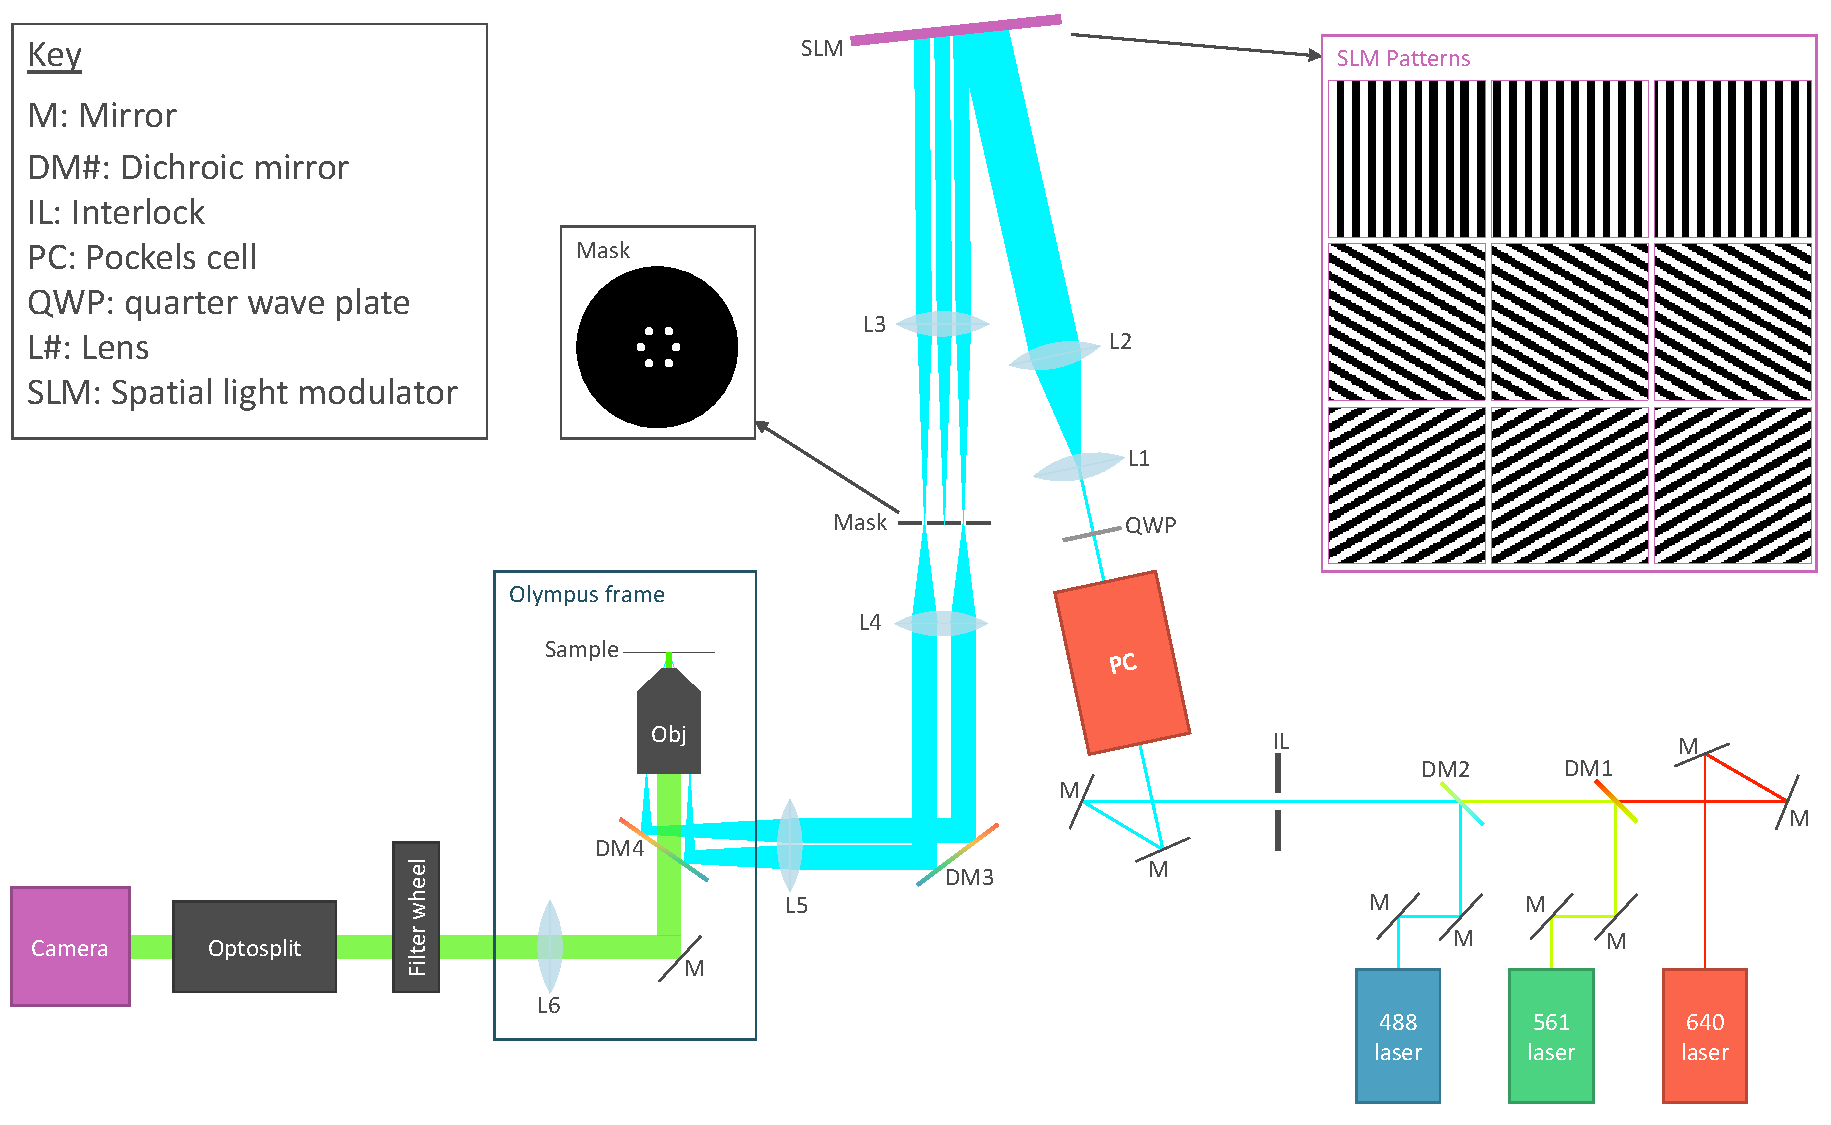
\includegraphics[width=0.92\textwidth]{sim-optical-path}
\caption[LAG SIM: Various optics work together to pattern the laser light with a SIM pattern and apply polarisation rotation for optical sectioning and resolution enhancement]{The optical layout of the SIM aligns light from one of 3 lasers onto an optical path. The light passes through a Pockels cell and quarter wave plate for polarisation rotation, before a square-wave pattern is applied by a spatial light modulator. The patterned light is passed through a spatial mask in the Fourier plane to produce a sinusoidal pattern, which is relayed onto the sample. The objective lens collects fluorescent emission light,  which is filtered to remove any reflected excitation light before reaching the sCMOS camera.}
\label{fig:SIMpath}
\end{sidewaysfigure}

The optical path diagram is shown in Figure~\ref{fig:SIMpath}, and works as follows: laser light is generated by one of three lasers at a wavelength of \SI{488}{\nano\metre}, \SI{561}{\nano\metre}, or \SI{640}{\nano\metre}; its polarisation is aligned with the direction of the structured illumination pattern by a Pockels cell and achromatic quarter-wave plate; it passes through a beam expander so that it fully covers the spatial light modulator (SLM) display; it reflects and diffracts off the SLM display, which is displaying a binary diffraction grating; it passes through a `beam minimiser' (a beam expander in reverse) so that it is an appropriate size for the microscope lenses; it passes through a spatial filter at a Fourier plane, which removes all but the ±1 diffraction orders from the SLM diffraction; it reflects off of a dichroic mirror; it passes into the microscope's tube lens; it reflects off of a second dichoric mirror; and finally it passes into the objective lens and is focussed onto the sample. 
DM3 and DM4 are sourced from the same manufacturing batch, so that any aberrations introduced by non-uniformity of DM3 are undone upon reflection from DM4. 

This effectively images a low-pass-filtered version of the SLM's diffraction grating onto the sample. 
The spatial filter means that the binary grating becomes a sinusoidal pattern, with the distance between peaks set by (a) the period of the diffraction grating shown on the SLM display and (b) the demagnification of the system from SLM to sample. 
An equivalent way of conceptualising this is to picture the two filtered beams of light entering the rear focal plane of the objective lens, such that they produce an interference pattern when they meet at the sample plane~\cite[\textit{ch. 9}]{hecht2017optics}. 
The result is a sinusoidal illumination pattern at the sample plane, the orientation and period of which can be set by binary patterns shown on the SLM. 

This SIM is a fluorescence microscope, so that, assuming linear fluorophore behaviour~\cite{gustafsson2005nonlinear, shen1984principles}, the amount of light emitted from a point in the sample is proportional to the amount of light illuminating that point, but the emission light is at a different wavelength to the illumination light. 
In the LAG SIM microscope, fluorescent emission light travels back through the objective lens, through the dichroic mirror and towards the camera to record a 2D image. 
Before it reaches the camera, it is filtered in one of two ways to remove any reflected illumination light.
The first option is to use a filter wheel, which contains three filters appropriate for removing the illumination light and can be switched via a serial command from the computer. 
The second option is to use the Optosplit III from Cairn Research, which uses filter cubes to split the emission light into three paths directed onto separate areas of the camera, facilitating simultaneous imaging of three colour channels.

The Optosplit provides a significant increase in speed for multicolour imaging. 
In this setup, the fastest speed at which the camera can reliably record images without dropping frames is \SI{10}{\milli\second}. 
A SIM reconstruction requires 9 images, giving a total exposure time of \SI{90}{\milli\second} per channel; however switching channels with the filter wheel adds an additional \SI{100}{\milli\second} as the wheel rotates to the next filter and settles. 
For a 3-colour image using the filter wheel, the fastest SIM imaging rate is therefore \SI{570}{\milli\second} per frame, or \SI{1.75}{\hertz}. 
Using the Optosplit is over 6 times faster, providing a maximum \SI{11.1}{\hertz} imaging rate even for multicolour images.

Finally, an autofocus system between the microscope frame and filter wheel works with the z-control of the microscope stage to maintain a constant focus on the sample. 
This is useful in two scenarios. 
Firstly, when a timelapse sequence is captured over a number of hours, the microscope lens drifts downwards away from the sample. 
Without the autofocus system, this would result in a loss of focus; however by automatically moving the stage as the lens drifts, focus can be maintained over a period of days.
Secondly, if a large field of view is captured to create a mosaic of images, focus can be lost due to the cover glass not being perfectly flat. 
Again, the autofocus system holds focus over this full field of view, allowing large areas to be imaged. 


\subsection{A Pockels cell provides fast polarisation rotation} \label{sec:lagsim-pockels}
In the SIM excitation path, a Pockels cell is used to rotate the polarisation of the illumination light so that it is aligned with the sinusoidal SIM pattern. 

In SIM, it is important that the modulation contrast is as large as possible, that is, that the troughs of the sinusoidal illumination pattern are as dark as possible.
When the 9 raw images are computationally recombined, the signal-to-noise ratio of high-spatial-frequency components is directly proportional to the modulation contrast~\cite{oholleran2012polarization}, as described in Section~\ref{sec:SIM-theory}. 

Modulation contrast of fluorescence emission light can be degraded by a number of sources, including out-of-focus light and aberrations in the imaging system, which is unavoidable in thick samples. 
Furthermore, if the polarisation of the illumination light is not rotated to align with the rotations of the SIM pattern,  modulation contrast is degraded due to the effects of a high numerical aperture lens. 

Two waves with orthogonal polarisation will not interfere~\cite{nityananda2013interference}. 
As light passes through a high numerical aperture lens, the polarisation state which is parallel to the meridional plane (p-polarised) is rotated; whereas the polarisation state perpendicular (s-polarised) is unaffected~\cite{mansuripur1991effects}. 
To ensure that light from the two beams entering the back-aperture of the lens arrive at sample plane with the same polarisation, it is therefore necessary that the light is entirely s-polarised~\cite{oholleran2012polarization}. 

If the meridional plane is defined at an angle of $\theta=0\si{\degree}$ around the optical axis, aligned with the back-aperture spots when the SLM is showing a vertical SIM grating pattern, the incident light should be linearly polarised at $\theta=90\si{\degree}$ to ensure s-polarised light, as shown in Figure~\ref{fig:meridional-plane}. 
However, for 2D isotropic resolution enhancement, the SIM pattern must also be rotated to $\pm60\si{\degree}$. 
For these patterns the $\theta=90\si{\degree}$ polarisation of the light does not represent s-polarised light. 
In order to maintain s-polarised light, thereby ensuring maximum pattern contrast, the polarisation must be rotated to align with each orientation of the SIM pattern. 

\begin{figure}[tbp]
\centering
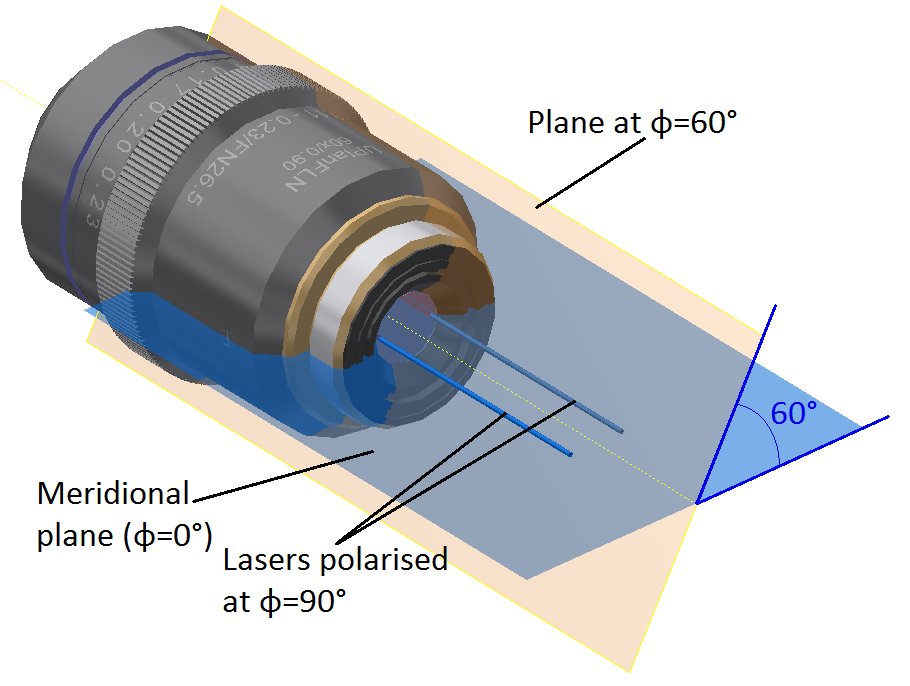
\includegraphics[width=\textwidth]{meridional-plane}
\caption[LAG SIM: Laser polarisation must be perpendicular to the sinusoidal illumination for high pattern contrast]{To ensure maximum pattern contrast, the excitation laser light must be s-polarised - that is, polarised at \SI{90}{\degree} to the meridional plane for the vertical sinusoidal illumination pattern. When the illumination pattern is rotated to $\pm60\si{\degree}$, $\theta=90\si{\degree}$ polarisation no longer produces s-polarised light. If the polarisation is not rotated to align with the rotated illumination pattern, some p-polarised light will enter the objective, which is rotated as it passes through the high NA lens. The p-polarised light will therefore not interfer at the sample plane, reducing the contrast of the illumination pattern.} \label{fig:meridional-plane}
\end{figure}

The original SIM system, detailed in reference~\cite{young2016guide}, used a liquid crystal variable retarder (LCVR) to rotate the polarisation to align with the SLM's grating orientation. 
This suffered an unexpected problem where the laser beam damaged the liquid crystal material leaving a visible spot on the LCVR and no longer retarded the light, so the system no longer rotated polarisation. 
The product line has since been discontinued.
As an interim solution, an achromatic half-wave plate was mounted in a serial-controlled rotation stage in place of the LCVR~\cite[\textit{ch. 8}]{hecht2017optics}. 
This setup successfully rotated the polarisation and ensured good modulation contrast, but was only able to image at \SI{0.1}{\hertz}. 

For fast and reliable polarisation rotation, facilitating \SI{11}{\hertz} SIM imaging, we purchased a Pockels cell from Conoptics. 
Similarly to the LCVR, a Pockels cell provides voltage-controlled retardation of one polarisation axis which, in combination with a quarter-wave plate, creates rotation of linear polarisation~\cite[\textit{ch. 8}]{hecht2017optics}.
The level of retardation is controlled by a voltage across the Pockels cell, restoring polarisation rotation with no mechanical movement. 

\subsection{Pockels cell alignment procedure} \label{sec:alignment-procedure}
To use the Pockels cell as a polarisation rotator, light entering the cell must be linearly polarised and aligned at \SI{45}{\degree} to the fast axis of the device. 
The Pockels cell from Conoptics Inc. was delivered with a Glan-Taylor polariser appropriately aligned in the factory. 

To align the Pockels cell to the rest of the system, the following procedure was devised, with the voltage across the Pockels cell set to \SI{0}{\volt}: % Shown in figure?
\begin{enumerate}
	\item Place the Pockels cell in 5-axis mount
	\item Coarsely align so that the beam passes through the centre of the Pockels cell
	\item Using a power meter after the Pockels cell, rotate the cell until power is maximised
	\item Adjust the tip-tilt of the Pockels cell, maximising power again
	\item Insert a linear polariser between the Pockels cell and power meter, and rotate until power is maximised
	\item Insert the quarter-wave plate (QWP) into the beam path mounted in a rotation mount between the Pockels cell and linear polariser
	\item With the power meter after the QWP, rotate the QWP until power is maximised, as shown in Figure~\ref{fig:alignment-photo}
	\item Remove the linear polariser
\end{enumerate}

Although this alignment procedure could be completed with any laser, for LAG SIM it is best to use the \SI{561}{\nano\metre} laser, as this is the closest to the centre wavelength of the achromatic quarter-wave plate. 

\begin{figure}[htbp!]
\centering
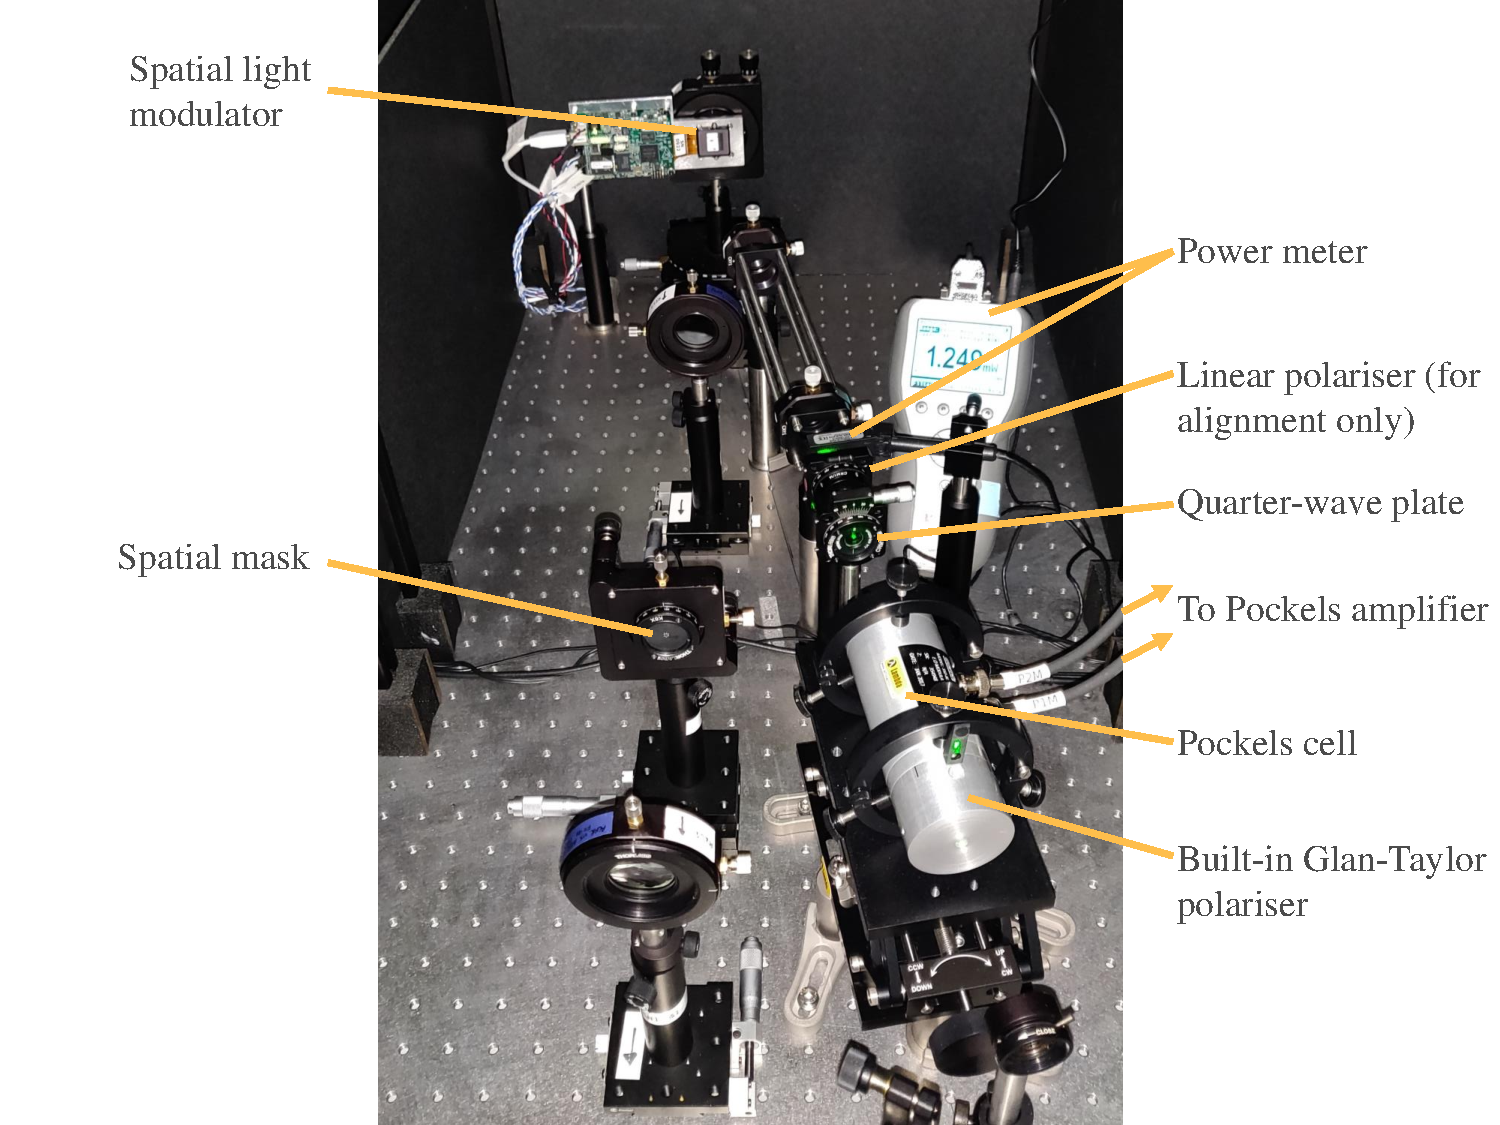
\includegraphics[width=1.0\textwidth]{alignment-photo}
\caption[LAG SIM: Alignment of the Pockels cell and quarter-wave plate to facilitate fast linear polarisation rotation]{The photo shows the LAG SIM beam path during alignment of the Pockels cell. A power meter is used in combination with a linear polariser to measure the polarisation rotation of the beam after retardation of one polarisation axis by the Pockels cell and quarter wave plate. Alignment is performed as per the protocol described in Section~\ref{sec:alignment-procedure}. Also visible are the spatial light modulator and spatial mask, which are used in combination to generate the sinusoidal illumination pattern.}
\label{fig:alignment-photo}
\end{figure}


The polarisation state of the light was measured to ensure the Pockels cell was behaving as expected by using a linear polariser in a rotation mount as an analyser before the power meter, as shown in Figure~\ref{fig:alignment-photo}. 
The laser emission entering the Pockels cell was linearly polarised, with an extinction ratio of 100:1 for the \SI{561}{\nano\metre} laser. 
The Glan-Taylor polariser theoretically increases the extinction ratio to >\num{100000}:1~\cite{bennett1995handbook}, although because it is attached to the Pockels cell in the factory, as seen in Figure~\ref{fig:alignment-photo} this extinction ratio cannot be measured. 
Light exiting the Pockels cell is elliptically polarised, with the degree of ellipticity determined by the voltage. 
Finally, the QWP restores the elliptically polarised light to linear polarisation, but rotated compared to the input as determined by the voltage over the Pockels cell.
The extinction ratio at the output of the QWP was 500:1. 

\subsection{Measuring Pockels cell voltages for optimal pattern contrast}
The voltage across the Pockels cell determines the amount of optical anisotropy in the cell~\cite[\textit{ch. 8}]{hecht2017optics}, which, in combination with a quarter wave plate, is directly proportional to the linear polarisation rotation. 
The voltages required to control anisotropy are of the order of \SI{100}{\volt}. 
To achieve these voltages, an amplifier supplied by Conoptics takes a \SIrange{-1}{1}{\volt} input and provides \SI[per-mode=symbol]{375}{\volt\per\volt} gain. 
The amplifier input voltage is generated by a National Instruments digital to analog converter (DAC), which is controlled by a LabVIEW program. 

\begin{figure}[b!]
\centering
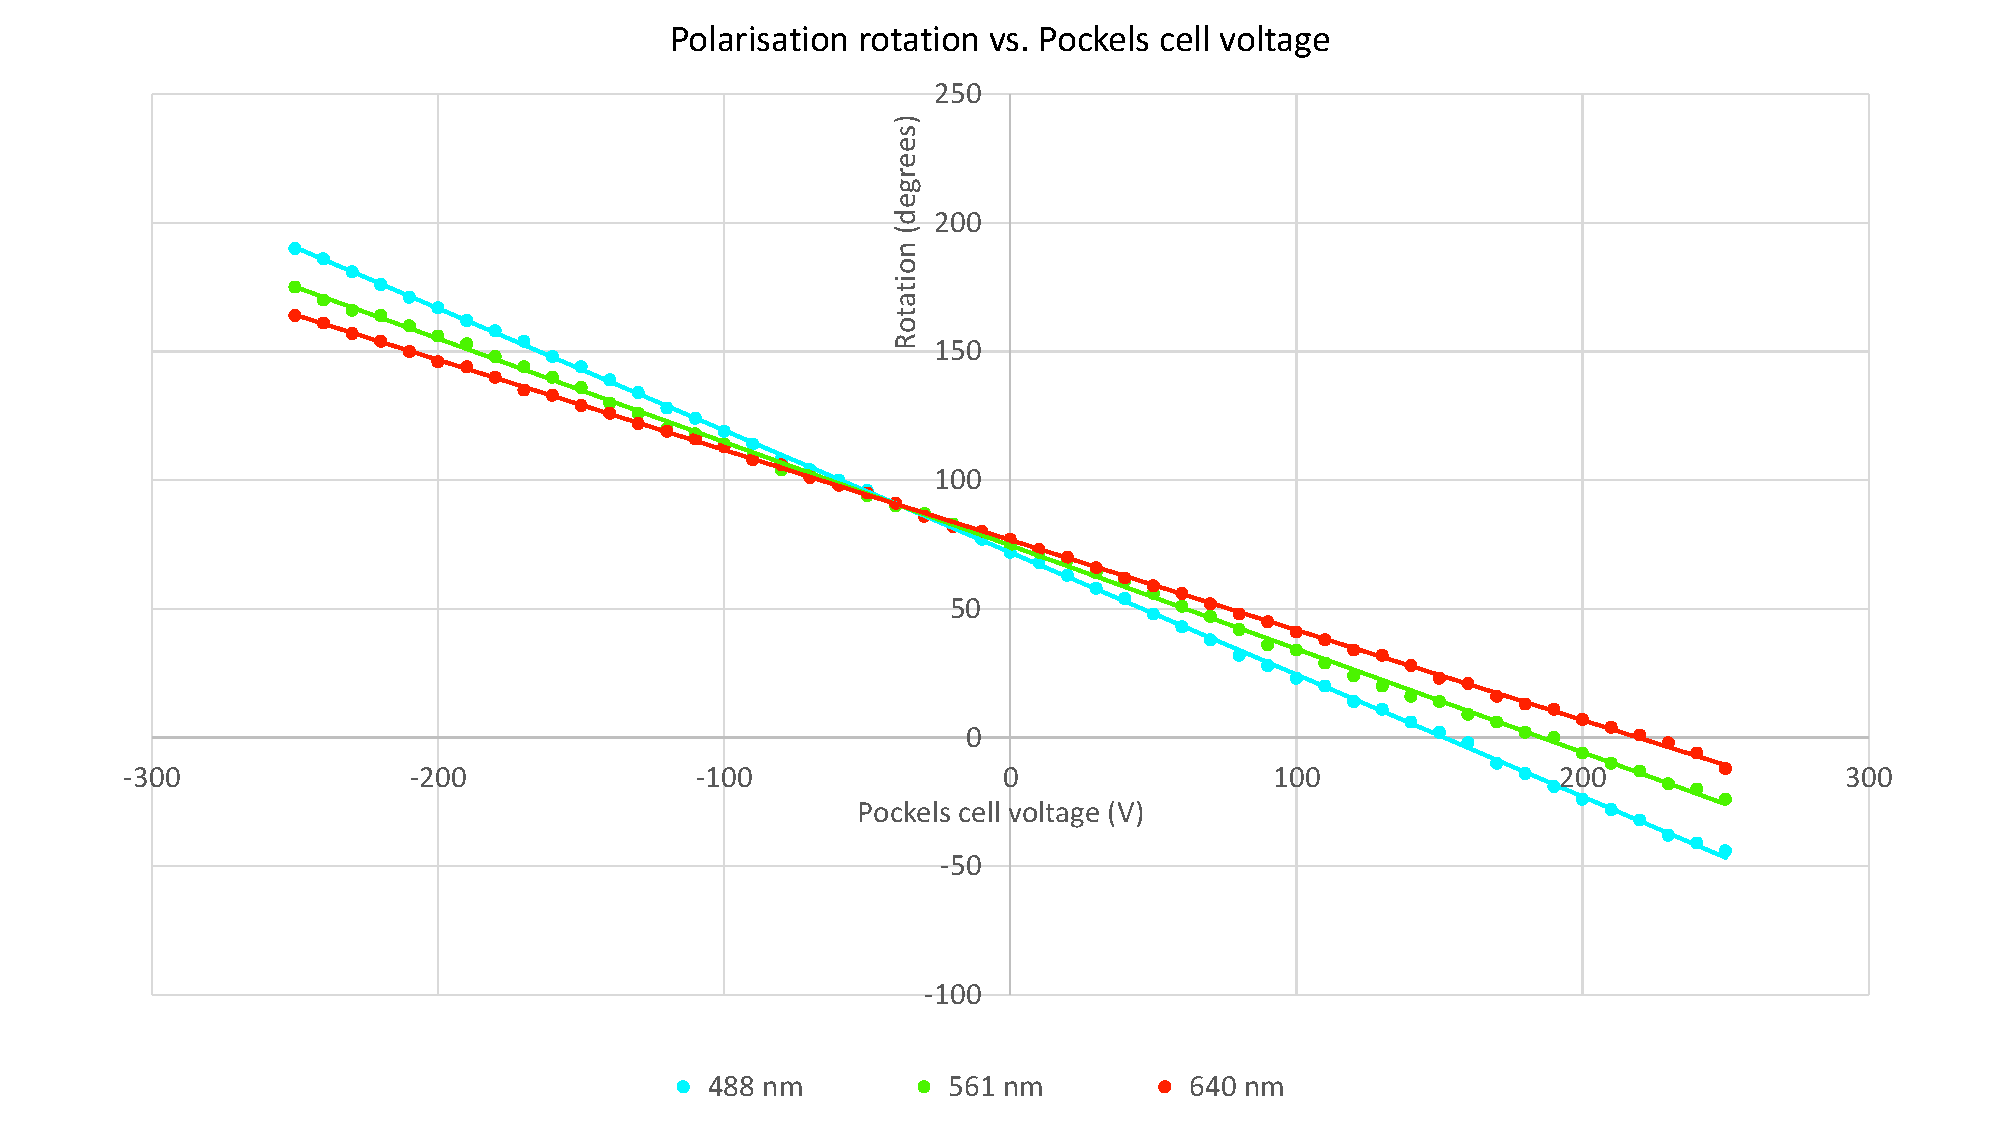
\includegraphics[width=1.0\textwidth]{pockels-voltage-vs-rotation}
\caption[LAG SIM: A Pockels cell is used to rotate the polarisation of laser light for maximum SIM pattern contrast]{When used in combination with a quarter wave plate, the voltage across the Pockels cell is proportional to polarisation rotation for each wavelength of laser light. Though the relationship is slightly different for each wavelength, at low voltages the values are similar enough that the~\SI{561}{\nano\metre} voltages can be used when the Optosplit is employed to image multiple channels simultaneously.}
\label{fig:pockels-voltage-rotation}
\end{figure}

Figure~\ref{fig:pockels-voltage-rotation} shows the relationship between voltage and polarisation rotation for the three laser lines used on the LAG SIM. 
Two useful properties of the Pockels cell are evident. 
Firstly, the Pockels cell is able to provide a full \SI{360}{\degree} polarisation rotation, more than adequate for the \SI{\pm60}{\degree} required to align polarisation with the SIM pattern orientations. 
Secondly, to achieve a given rotation a similar voltage is required for all wavelengths. 

To measure pattern contrast at a given voltage, images of sub-diffraction beads were recorded under sinusoidal SIM illumination. 
Beads located in a trough of the pattern were dark; conversely beads lying in a peak were bright. 
At each voltage step the phase of the illumination pattern was swept so that, at some point during the phase sweep, each bead passed through a peak and a trough. 
Calculating the difference between the maximum and minimum brightness for each bead provides a measure of pattern contrast for a given voltage. 

To calculate the voltages required to achieve maximum pattern contrast at each wavelength and orientation, a LabVIEW program was written to sweep the Pockels cell voltage in steps of \SI{25}{\volt}. 
Pattern contrast was measured at each voltage, shown in Figure~\ref{fig:pockels-contrast}. 
Each orientation of the illumination pattern has a different voltage which gives a peak contrast. 
The optimal pattern contrast measurement was repeated for each pattern orientation at each wavelength, as shown in Figure~\ref{fig:pockels-optimal}. 
%The contrast measurement was repeated around each peak to find the optimal contrast voltage to the nearest \SI{1}{\volt}, shown inset on Figure~\ref{fig:pockels-contrast}. 

\begin{figure}[htbp!] 
\centering
\begin{subfigure}[b]{\textwidth}
	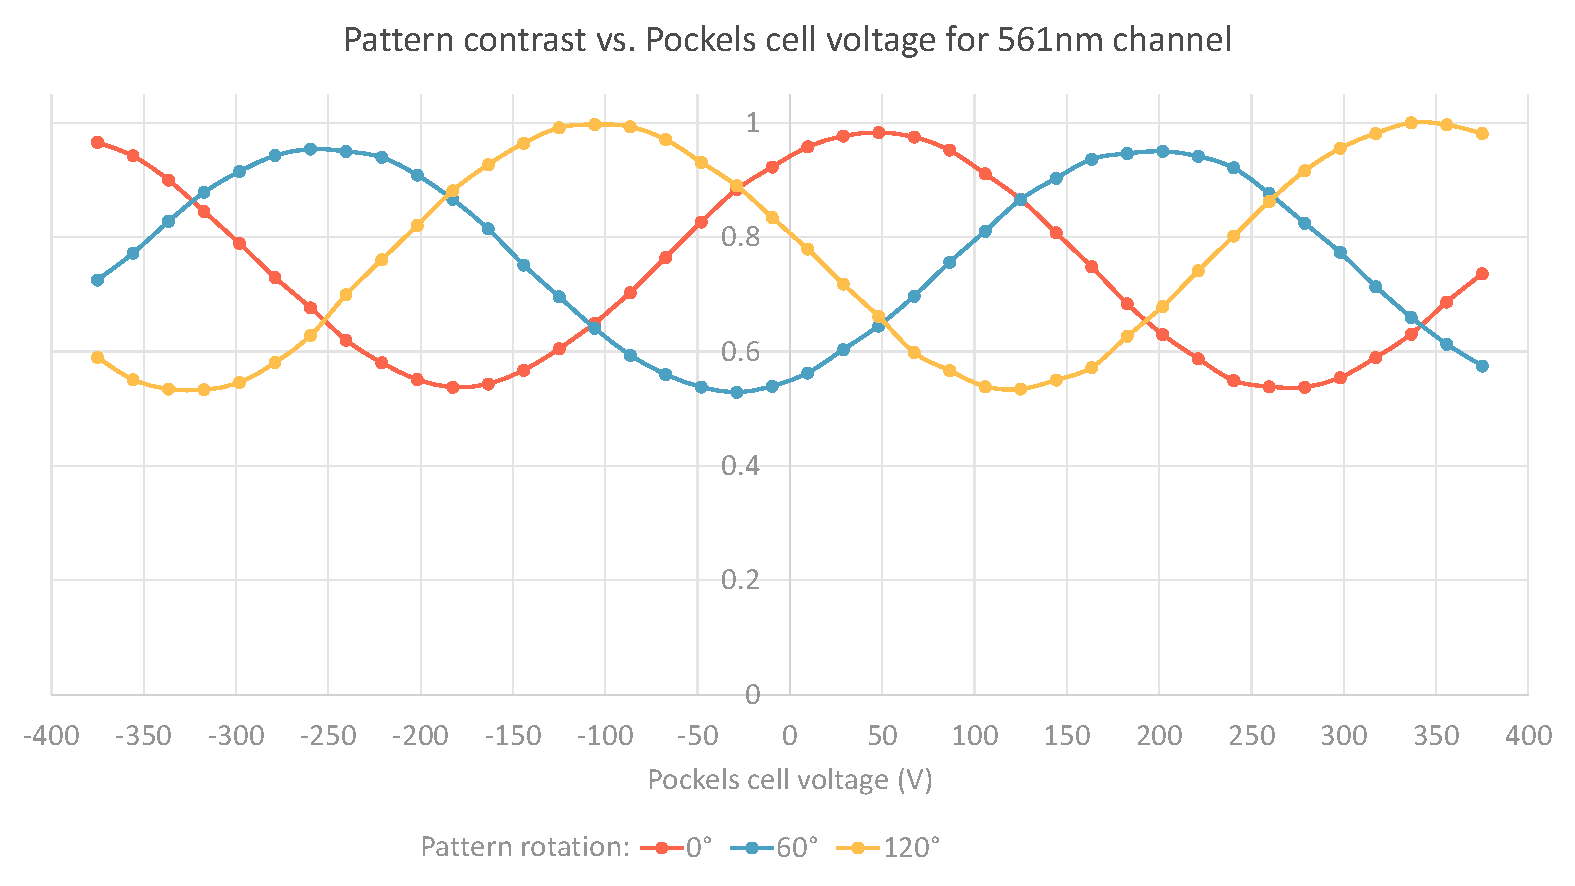
\includegraphics[width=1.0\textwidth]{pockels-contrast}
	\caption{}\label{fig:pockels-contrast}
\end{subfigure}
\begin{subfigure}[b]{\textwidth}
	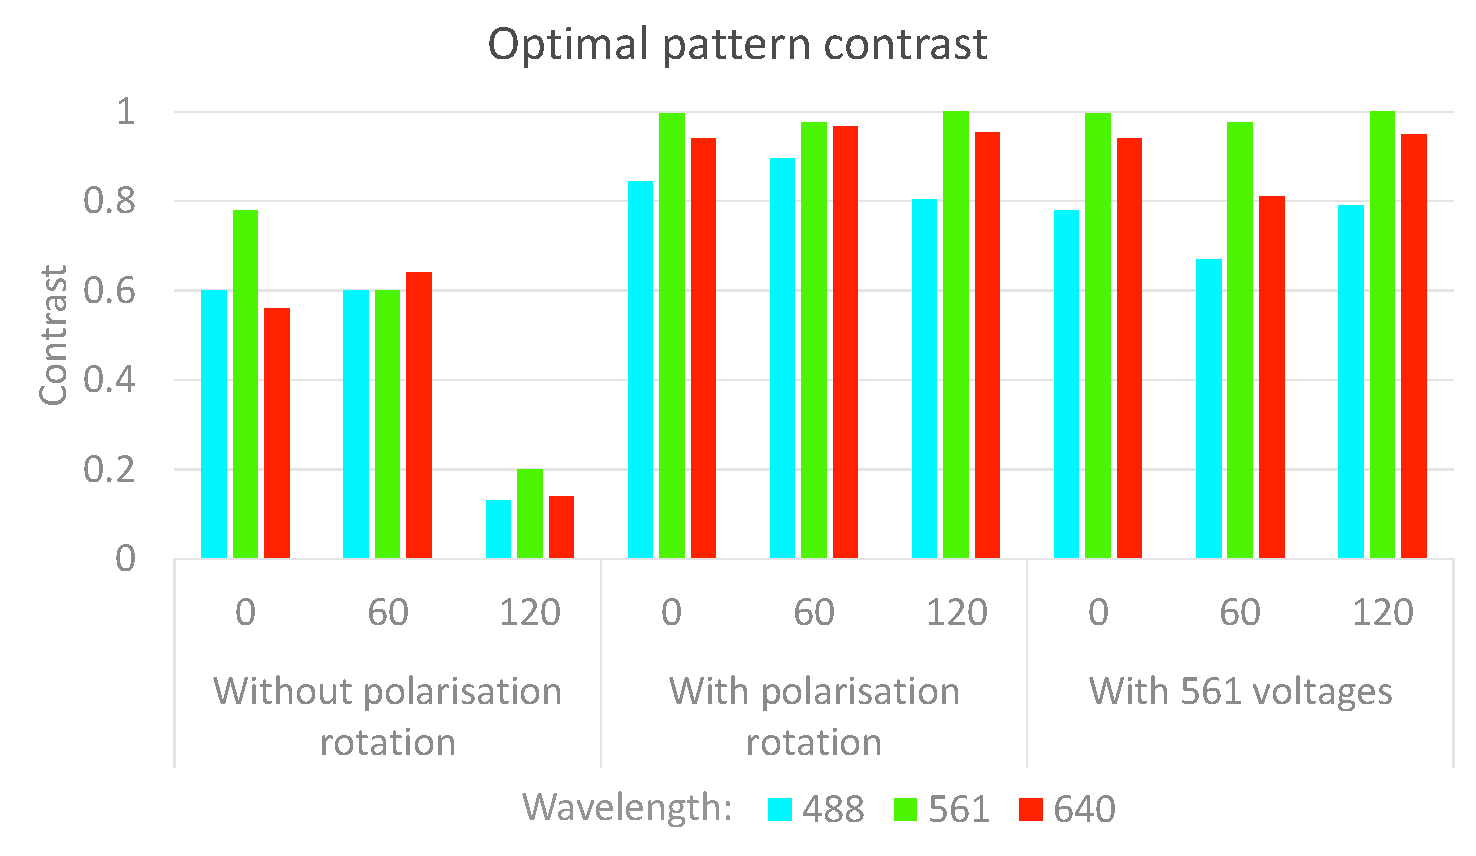
\includegraphics[width=\textwidth]{pockels-rotations}
	\caption{}\label{fig:pockels-optimal}
\end{subfigure}
\caption[LAG SIM: Measurements of a bead sample reveal the optimal Pockels cell voltages for maximum pattern contrast]{(a) shows the pattern contrast, measured on a \SI{100}{\nano\metre} bead sample, as the voltage was swept from \SIrange{-375}{375}{\volt} to find the voltage which gave maximum contrast. The process was repeated for each rotation of the sinusoidal SIM pattern, and for each wavelength of light. (b) shows that rotating polarisation leads to high pattern contrast for all rotations and wavelengths. Furthermore, since the required voltage to achieve a given rotation is similar for all wavelengths, using the \SI{561}{\nano\metre} voltages allows for imaging multiple channels simultaneously whilst maintaining a high pattern contrast.}
\label{fig:pockels-contrast-figures}
\end{figure} 

Without polarisation rotation, optimum pattern contrast cannot be achieved, and is almost at a minimum for the \SI{120}{\degree} pattern orientation. 
Performing SIM without polarisation rotation would introduce significant artefacts in the reconstruction, as low modulation contrast translates into low signal-to-noise ratio of high frequency components, as described in Section~\ref{sec:SIM-theory}.
Furthermore the signal-to-noise ratio would vary in each orientation, producing an OTF and corresponding PSF which is not rotationally symmetric, adding more artefacts to the reconstructed image.

When the Pockels cell is used to rotate polarisation, a high pattern contrast can be achieved in all orientations of the illumination pattern at each wavelength. 
This corresponds to a high modulation depth $m$ in Equation~\ref{eq:matrix-solved}, translating directly into high signal-to-noise ratio for high frequency components and facilitating artefact-free SIM reconstruction with 2$\times$ resolution enhancement. 

Furthermore, because the voltages to achieve a given polarisation rotation are similar for all wavelengths, the polarisation of all three laser wavelengths can be rotated simultaneously using the \SI{561}{\nano\metre} optimal voltages. 
Figure~\ref{fig:pockels-optimal} shows that a high pattern contrast is still maintained for each wavelength in this scheme. 
This facilitates use of the Optosplit for simultaneous 3-channel SIM imaging, providing multi-colour resolution enhancement over 6$\times$ faster than capturing channels separately and switching emission filters with a filter wheel. 

\section{LabVIEW hardware control} \label{sec:labview}
\subsection{Control requirements for SIM imaging} \label{sec:SIMsteps}
The LAG SIM has a number of hardware components which must all work together to acquire a set of images appropriate for SIM reconstruction.
Specifically, the following sequence of events must take place:
\begin{enumerate}
	\item Set filter wheel to correct position for the excitation and emission wavelengths
	\item\label{step:pockels} Set voltage across Pockels cell for correct polarisation rotation
	\item Set SLM pattern to the correct orientation and phase
	\item Turn on the laser
	\item Open the camera shutter for the exposure time
	\item Close the camera shutter
	\item Turn off the laser
	\item\label{step:record} Record the image
\end{enumerate}
Steps \ref{step:pockels} to \ref{step:record} must be repeated for each of the 9 illumination patterns, and the entire process then repeated for additional colour channels if the Optosplit is not being utilised. 
For a time series, this entire process must then be repeated for the required number of frames; for a z-stack, the distance from the stage to the lens must also be adjusted before repeating the process. 

The original SIM, detailed in~\cite{young2016guide}, used a separate software program for controlling each piece of hardware. 
This caused a number of problems: firstly, setting up experiments was a complicated process prone to human errors, due to the number of parameters which had to be correctly entered in separate programs; and secondly, making modifications to the imaging parameters during an imaging session was difficult and time-consuming. 
When imaging live-cell biology, there is a real impetus to image quickly, as cells become unhealthy and soon die on the microscope stage. 

Furthermore, the complicated system meant that only one person in the LAG had the knowledge to gather images from the SIM. 
This meant that any biological experiments which would benefit from SIM required my direct supervision, so that many projects were not able to use the SIM, and that I personally had little time for my other research aims.
There was a clear need for a new, unified SIM interface, which could be used by non-expert users with minimal training. 

\subsection{A user-friendly LAG SIM interface enables operation by non-expert users}
The new interface was built in LabVIEW. 
Although each hardware component came with its own control software, all components could also be controlled either through serial commands, analog voltages, or transistor-transistor logic (TTL) levels. 
As a graphical language with hardware control in mind, LabVIEW provides easy-to-use built-in blocks to fulfil each of these functions, as well as a clear visual representation of a sequence of control events.
Furthermore it makes designing user interfaces a straightforward process, allowing a programmer to create a user-friendly program for the end user. 
This made LabVIEW an ideal candidate for building an accessible program for controlling the LAG SIM.

The LAG SIM interface is shown in Figure~\ref{fig:lagsimLabview}.
The key functions are located in the Live Mode area and the Acquire tab, although for the sake of completeness each tab is detailed in this section. 

\begin{figure}[p]
\centering
\begin{subfigure}[b]{0.6\textwidth}
	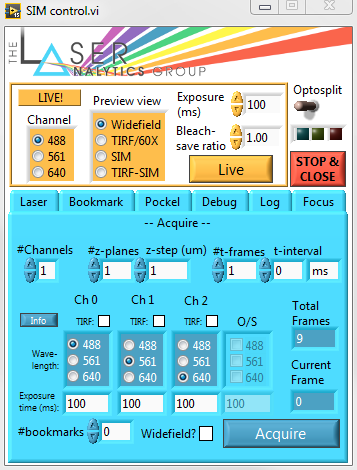
\includegraphics[width=\textwidth]{lagsimLabviewAcq}
	\caption{}\label{fig:fpbLabviewAcq}
\end{subfigure}

~\newline
\begin{subfigure}[b]{1.0\textwidth}
	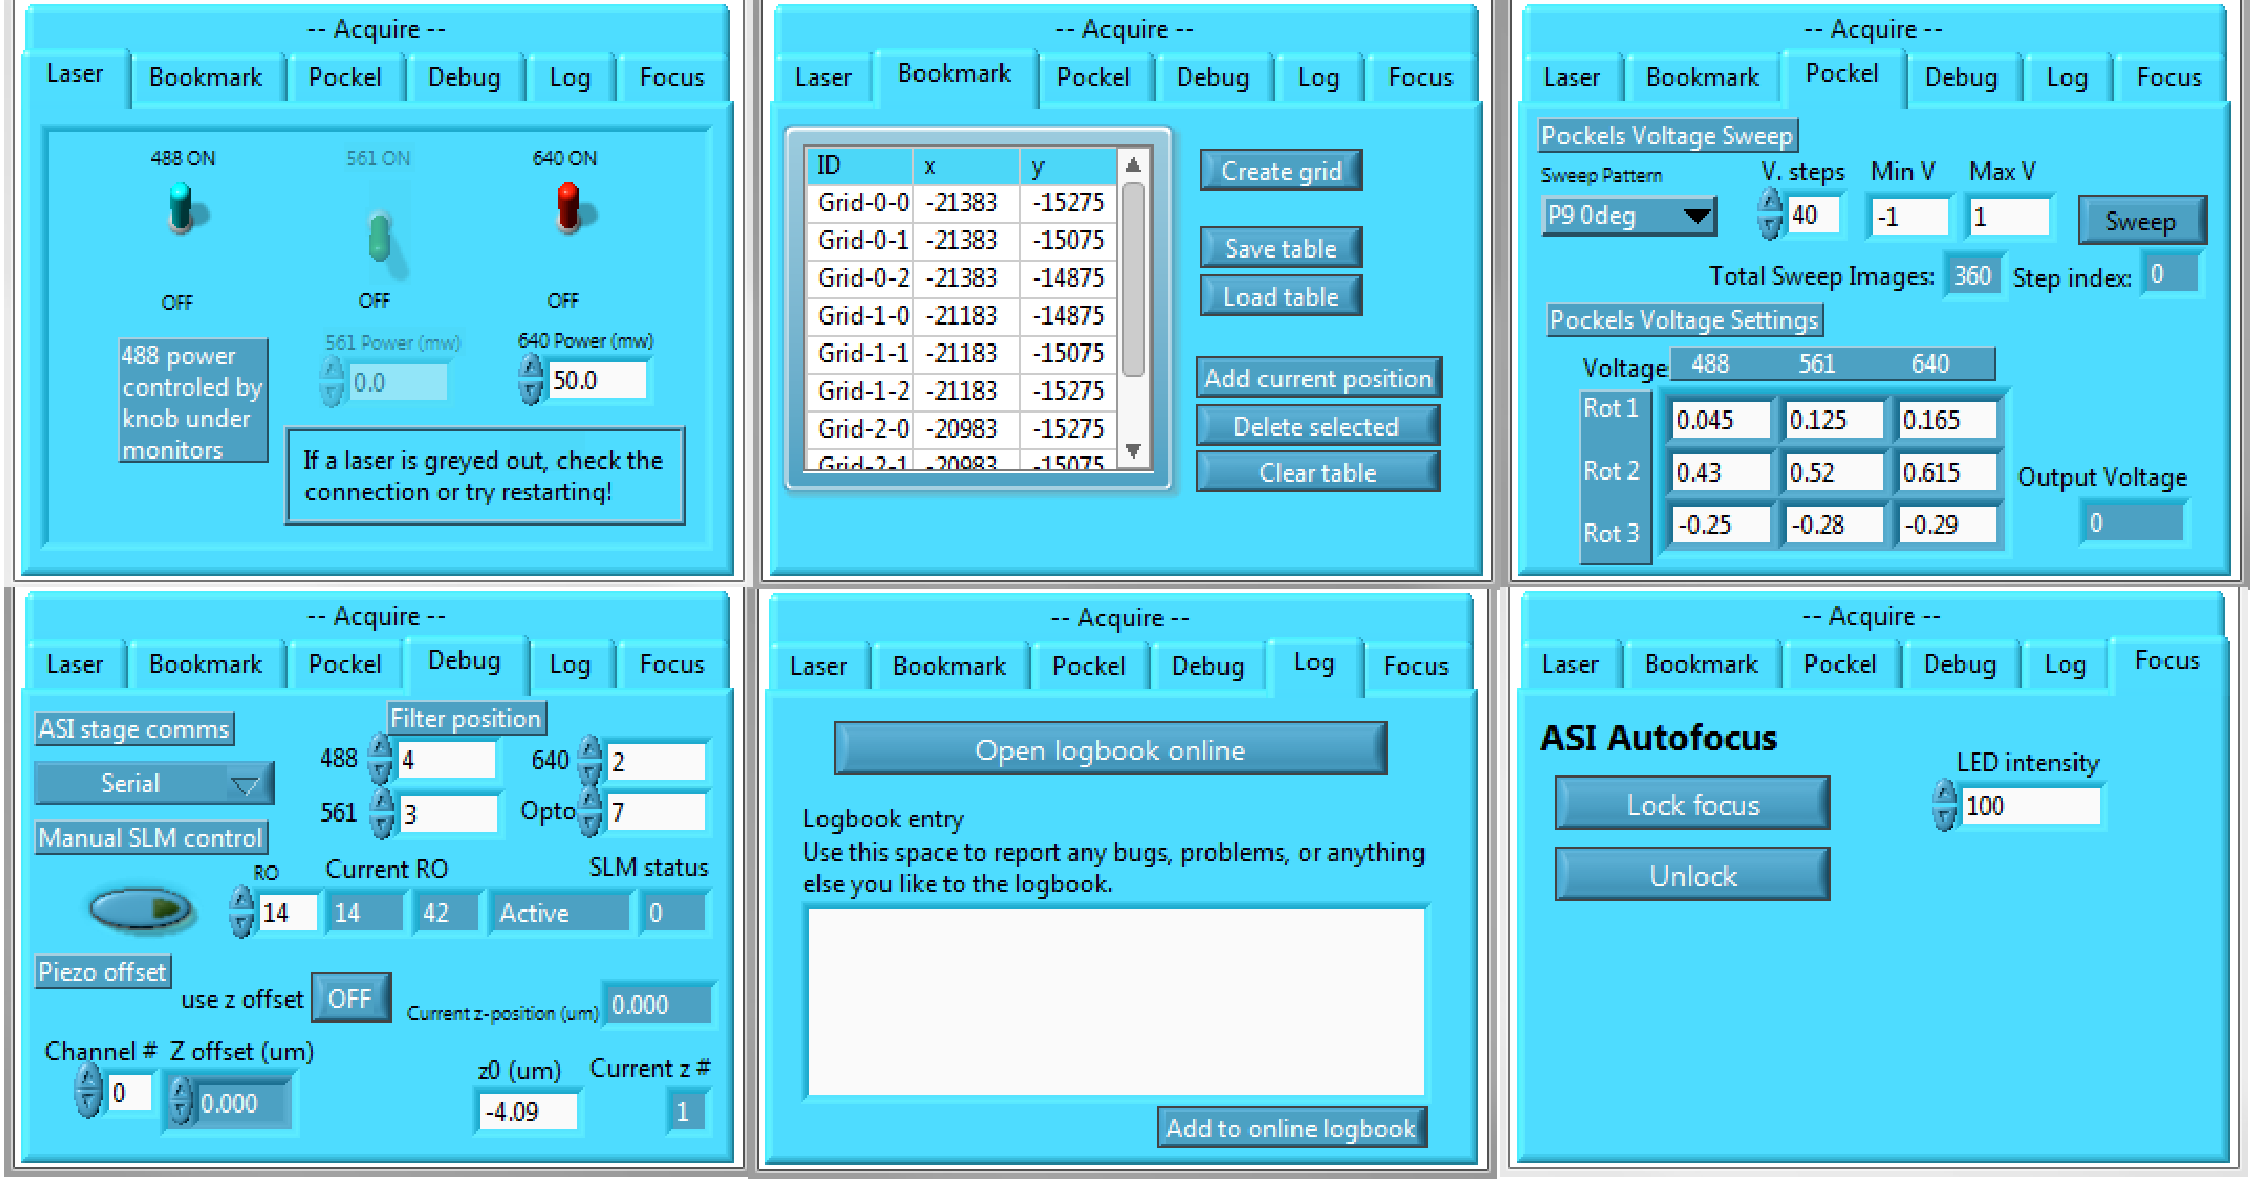
\includegraphics[width=\textwidth]{lagsimLabviewOthers}
	\caption{}\label{fig:fpbLabviewTabs}
\end{subfigure}
\caption[LAG SIM: The LabVIEW user interface for controlling LAG SIM is designed for operation by non-expert users]{The LabVIEW user interface used to control the LAG SIM has been designed for operation by a non-expert user, with advanced tasks hidden in the extra tabs shown in (b). } % Needs a few more words actually 
\label{fig:lagsimLabview}
\end{figure}

\subsection{Live tab for fast image preview} \label{sec:lagsimLive}
The live tab is always visible whenever the LAG SIM Control software is open. 
It works in conjunction with the HCImage camera software provided by Hamamatsu, which provides a live display of the camera chip. 

In live mode, the illumination wavelength can be changed with the radio buttons or with the F2, F3 and F4 keys for fast, mouse-free operation. 
This allows users to quickly identify cells in one channel, for example with a fluorescent nucleus marker, and confirm presence of another marker in the second channel.
This fast channel switching minimises photobleaching when panning for healthy cells to image in detail. 
% This is surprisingly useful, see supplementary video? 

Another live-mode feature designed to reduce bleaching is the so-called `bleach-save ratio.' 
This is a number between 0 and 1 which switches off the laser for a fraction of the exposure time. 
By setting the exposure time and bleach-save ratio as small as possible while still being able to find healthy cells, the level of light the sample is exposed to can be minimised.
This is especially important in live-cell biology, where excess light can cause phototoxic effects bringing about cell death. 

The illumination pattern used for live mode will usually be a pseudo-widefield mode, which emulates widefield illumination by dithering all three phases of a SIM pattern over one exposure time of the camera. 
True epi-illumination is not possible on the LAG SIM due to the spatial mask, which blocks the 0-order diffraction spot in the Fourier plane. 
The user can also choose to preview the SIM pattern by selecting the appropriate radio button; if the stripe pattern is visible, this is a good indication that later reconstruction into a resolution-enhanced image will be successful. 
If the \SI{1.49}{\numaperture} TIRF lens is used, then selecting the TIRF radio button sets the SLM pattern such that the ±1 diffraction spots hit the TIRF ring on the objective back aperture, leading to TIRF illumination at the sample. 
This can be done with the SIM pattern visible or in a dithered mode, as with non-TIRF illumination. 

The Optosplit rocker in the control software sets the system up for imaging with the Cairn Optosplit III. 
The Optosplit is a device on the output port of the microscope which contains two filter cubes and a set of mirrors so that each channel can be imaged simultaneously onto a separate 512$\times$512 area of the 2048$\times$2048 camera chip.
When the filter cubes are removed, and the Optosplit rocker is in the \texttt{OFF} position, the Optosplit has no effect and channels are imaged sequentially, with an appropriate filter for each channel loaded into position by the filter wheel. 
With Optosplit mode \texttt{ON}, however, the live-mode channel selection radio buttons become checkboxes, so that each colour channel can be switched on and off independently. 
The Optosplit provides much faster imaging speeds, at the potential cost of cross-talk between colour channels. 

% Should actually move most of this up? and just talk about the user interface here, maybe about assessing bleedthrough from shorter wavelengths to longer ones

This upper section of the user interface contains two more important components. 
A laser status indicator shows which lasers are currently exposing, an important safety feature so that users know it is safe to remove their sample after an imaging session. 
The \texttt{STOP \& CLOSE} button safely exits the control software, ensuring that the lasers are switched off, the camera is finished exposing, and the voltage across the Pockels cell is set to \SI{0}{\volt}. 
To ensure that this exit sequence runs when a user has finished their imaging session, the `\texttt{X}' close button in the window's title bar is disabled. 

\subsection{Acquire tab facilitates multi-dimensional imaging}
Once a healthy cell with the required staining has been located from live mode, it can be captured as a SIM image with the Acquire tab. 
With the default settings shown in Figure~\ref{fig:fpbLabviewAcq}, this will capture a set of 9 raw SIM images following the steps described in Section~\ref{sec:SIMsteps}.
Additional settings in this tab allow a set of images to be captured for 3D z-stacks, timelapse imaging, and other multi-image acquisitions. 

If the number of \texttt{z-steps} is greater than 1, then the ASI stage will move in the axial direction at the end of every SIM acquisition by the value given in the \texttt{z-step} box. 
Since the axial resolution of the SIM is \SI{440}{\nano\meter}, for a Nyquist-limited z-stack a \texttt{z-step} of \SI{200}{\nano\meter} should be used. 

To take a series of images over time, the \texttt{t-frames} parameter should be set to greater than 1.
For observing fast, dynamic events, the \texttt{t-delay} parameter should be set to \SI{0}{\milli\second}. 
Timelapse imaging, for example capturing an image every minute for an hour, can be achieved by setting the \texttt{t-delay} to \SI{60}{\second}, which will pause the software for the given amount of time at the end of each acquisition. 

Multi-channel imaging can be achieved either with or without the Optosplit. 
If the Optosplit switch is set \texttt{OFF}, and the number of channels is set to more than 1, the filter wheel will rotate the correct filter into position after each channel is captured. 
The exposure time of each raw SIM frame can be set per-channel, and the channel order can be changed with the radio buttons. 

Faster imaging can be achieved with the Optosplit. 
This sets the filter wheel to an empty filter, and filtering is performed with filter cubes in the Optosplit. 
In this mode, the choice of channels is controlled with checkboxes. 

The bookmarks number should be set to the number of bookmarks in the bookmarks table, or a lower number $N$ if the user only wants to capture the first $N$ bookmarked locations from the table. 
If bookmarks are not to be used, this value should be left at 0 - a value of 1 will move to the first bookmark listed in the bookmark table and capture an image there. 
Bookmarks are discussed in more detail in Section~\ref{sec:lagsimBookmarks}. 

The LAG SIM microscope can be used to capture images in a pseudo-widefield mode, by dithering the SIM pattern as described in Section~\ref{sec:lagsimLive}. 
This is enabled by ticking the \texttt{Widefield} checkbox. 
This will enable imaging with widefield resolution at the camera's maximum acquisition speed of \SI{100}{\hertz}. 

Once the appropriate variables have been set for the acquisition, the total frames is displayed in the \texttt{Total frames} box. 
This number should be entered into the HCImage camera software, to prepare the camera for a high-speed image acquisition. 
Once the user has pressed \texttt{Start} in the HCImage software, the camera buffer is ready to receive images; then pressing \texttt{Acquire} in the LAG SIM software starts the acquisition process. 

A future version of the software could automate this final step, eliminating the need for the HCImage software.
This would require synchronised access to the camera data stream through LabVIEW. 


\subsection{Laser tab provides safe power control}
Laser control is integrated into the LAG SIM control software. 

At the launch of the software, the controls are greyed-out and disabled. 
When LabVIEW successfully connects to each laser, its controls become enabled, to switch the lasers on and off and change the power. 
Lasers are switched off automatically when the software is closed, for added safety when the microscope is unattended. 

Having fast and straightforward access to laser control is particularly useful for reducing light dosage in live mode.
Power can then be increased for acquisition to obtain the highest possible image quality. 

\subsection{Bookmark tab for saving positions and creating mosaics} \label{sec:lagsimBookmarks}
The LAG SIM LabVIEW program is able to store locations on the microscope slide as bookmarks.
If the number of bookmarks in the \texttt{Acquire} tab is set to greater than 0, the microscope stage will move before each acquisition to the next bookmarked position in the bookmark table. 
This is especially useful for imaging a collection of cells over a long period of time. 

The SIM user can pan around the microscope slide in \texttt{live mode} searching for healthy cells with good fluorescent labelling, and save them to the bookmark table by clicking \texttt{Add bookmark}. 
The location can be returned to by double-clicking on the table entry, or acquired sequentially and repeatedly in the \texttt{Acquire} tab. 

Furthermore this tab contains an option for creating bookmarks in a grid pattern. 
This can be utilised for imaging large areas, which are then stitched together to form one large mosaic image, for example the whole mouse brain shown in Figure~\ref{fig:wholebrain}. 

\begin{figure}[p]
\centering
\includegraphics[angle=90, width=1.0\textwidth]{whole-brain}
\caption[LAG SIM: An image of a full mouse brain can be captured as a mosaic of images]{The bookmark mode offered by LAG SIM can be used to create tiled images, such as this 3-colour image of a mouse brain. Dissection and staining performed by Sarah F{\"o}rster. Scalebar is \SI{500}{\micro\metre}}
\label{fig:wholebrain}
\end{figure}

\subsection{Focus tab controls the autofocus} \label{sec:lagsimFocus}
Using the grid bookmark function to image large fields of view can fail if the coverglass or microscope stage is not perfectly flat, which is often the case in practical experiments. 
To keep the focus locked at the same distance from the sample, the `Lock focus' button begins the autofocus procedure. 
Assuming the autofocus sensor receives enough reflected signal from the infrared autofocus light emitting diode (LED), the sample will be locked at a fixed distance from the objective lens. 
If not, an error message is returned requesting the user to increase the LED power for a stronger signal. 
The system can also be used to maintain focus over a time period of hours to days, even as the objective lens drifts away from the sample. 

The autofocus is switched off with the `Unlock focus' button, releasing z-control back to the user. 

\subsection{Pockels tab to find optimal voltages for maximum pattern contrast} 
The Pockels cell retards one polarisation axis by an amount dependent on the voltage across it. 
In combination with a quarter wave plate, this allows for linear polarisation rotation necessary for the high pattern contrast required for SIM, explained in Section~\ref{sec:lagsim-pockels}. 
The amount of retardation depends on the wavelength of light, therefore different wavelengths require different voltages to achieve the same polarisation rotation. 

To find the optimum voltage for each wavelength, functionality is implemented in the \texttt{Sweep} tab to sweep the voltage from \SIrange{-1}{1}{\volt}, in a number of voltage steps. 
At each voltage, the SIM pattern's phase is swept and pattern contrast can be measured using a diffraction-limited bead sample. 
Pattern contrast is calculated with a MATLAB script to produce the graph in Figure~\ref{fig:pockels-contrast}, showing how pattern contrast changes with voltage. 

This gives a coarse estimation of the voltage required to achieve maximum pattern contrast. 
The sweep limits can then be adjusted to a small amount either side of the coarse estimation's maximum contrast to obtain a more accurate voltage. 

This process must be repeated for each wavelength, and each rotation of the SIM pattern. 
Once the process is complete, the optimum voltages can be entered into the table, and will be applied to the Pockels cell during a SIM acquisition. 


\subsection{Debug tab contains alignment options and other advanced features}
A number of advanced user options are contained in the \texttt{Debug} tab. 
These extend the functionality of the microscope for non-conventional uses including alignment. 

The emission filters in the filter wheel change with excitation wavelength for use with commercially available fluorophores.
However, some samples - such as semiconducting perovskites - emit around \SI{750}{\nano\metre} when excited with \SI{488}{\nano\metre} light. 
Unconventional filters can be selected in this tab to image these samples. 

Manual SLM control gives the user direct control over the pattern displayed on the SLM. 
This means specialised patterns, such as a SIM pattern masked by a circle, or even 3 SIM patterns with different orientations overlayed, can be used.
These types of patterns are particularly useful for alignment of the system: overlaying 3 orientations of the SIM pattern produces 6 spots at the Fourier plane, which must be centred around the optical axis; therefore a coarse alignment can be performed using a translucent pinhole alignment tool on the microscope, as shown in Figure~\ref{fig:pinhole-alignment}. 
A fine alignment is then performed using the masked patterns, by ensuring the two circles overlap at the focal plane of the microscope. 

\begin{figure}[htbp!]
\centering
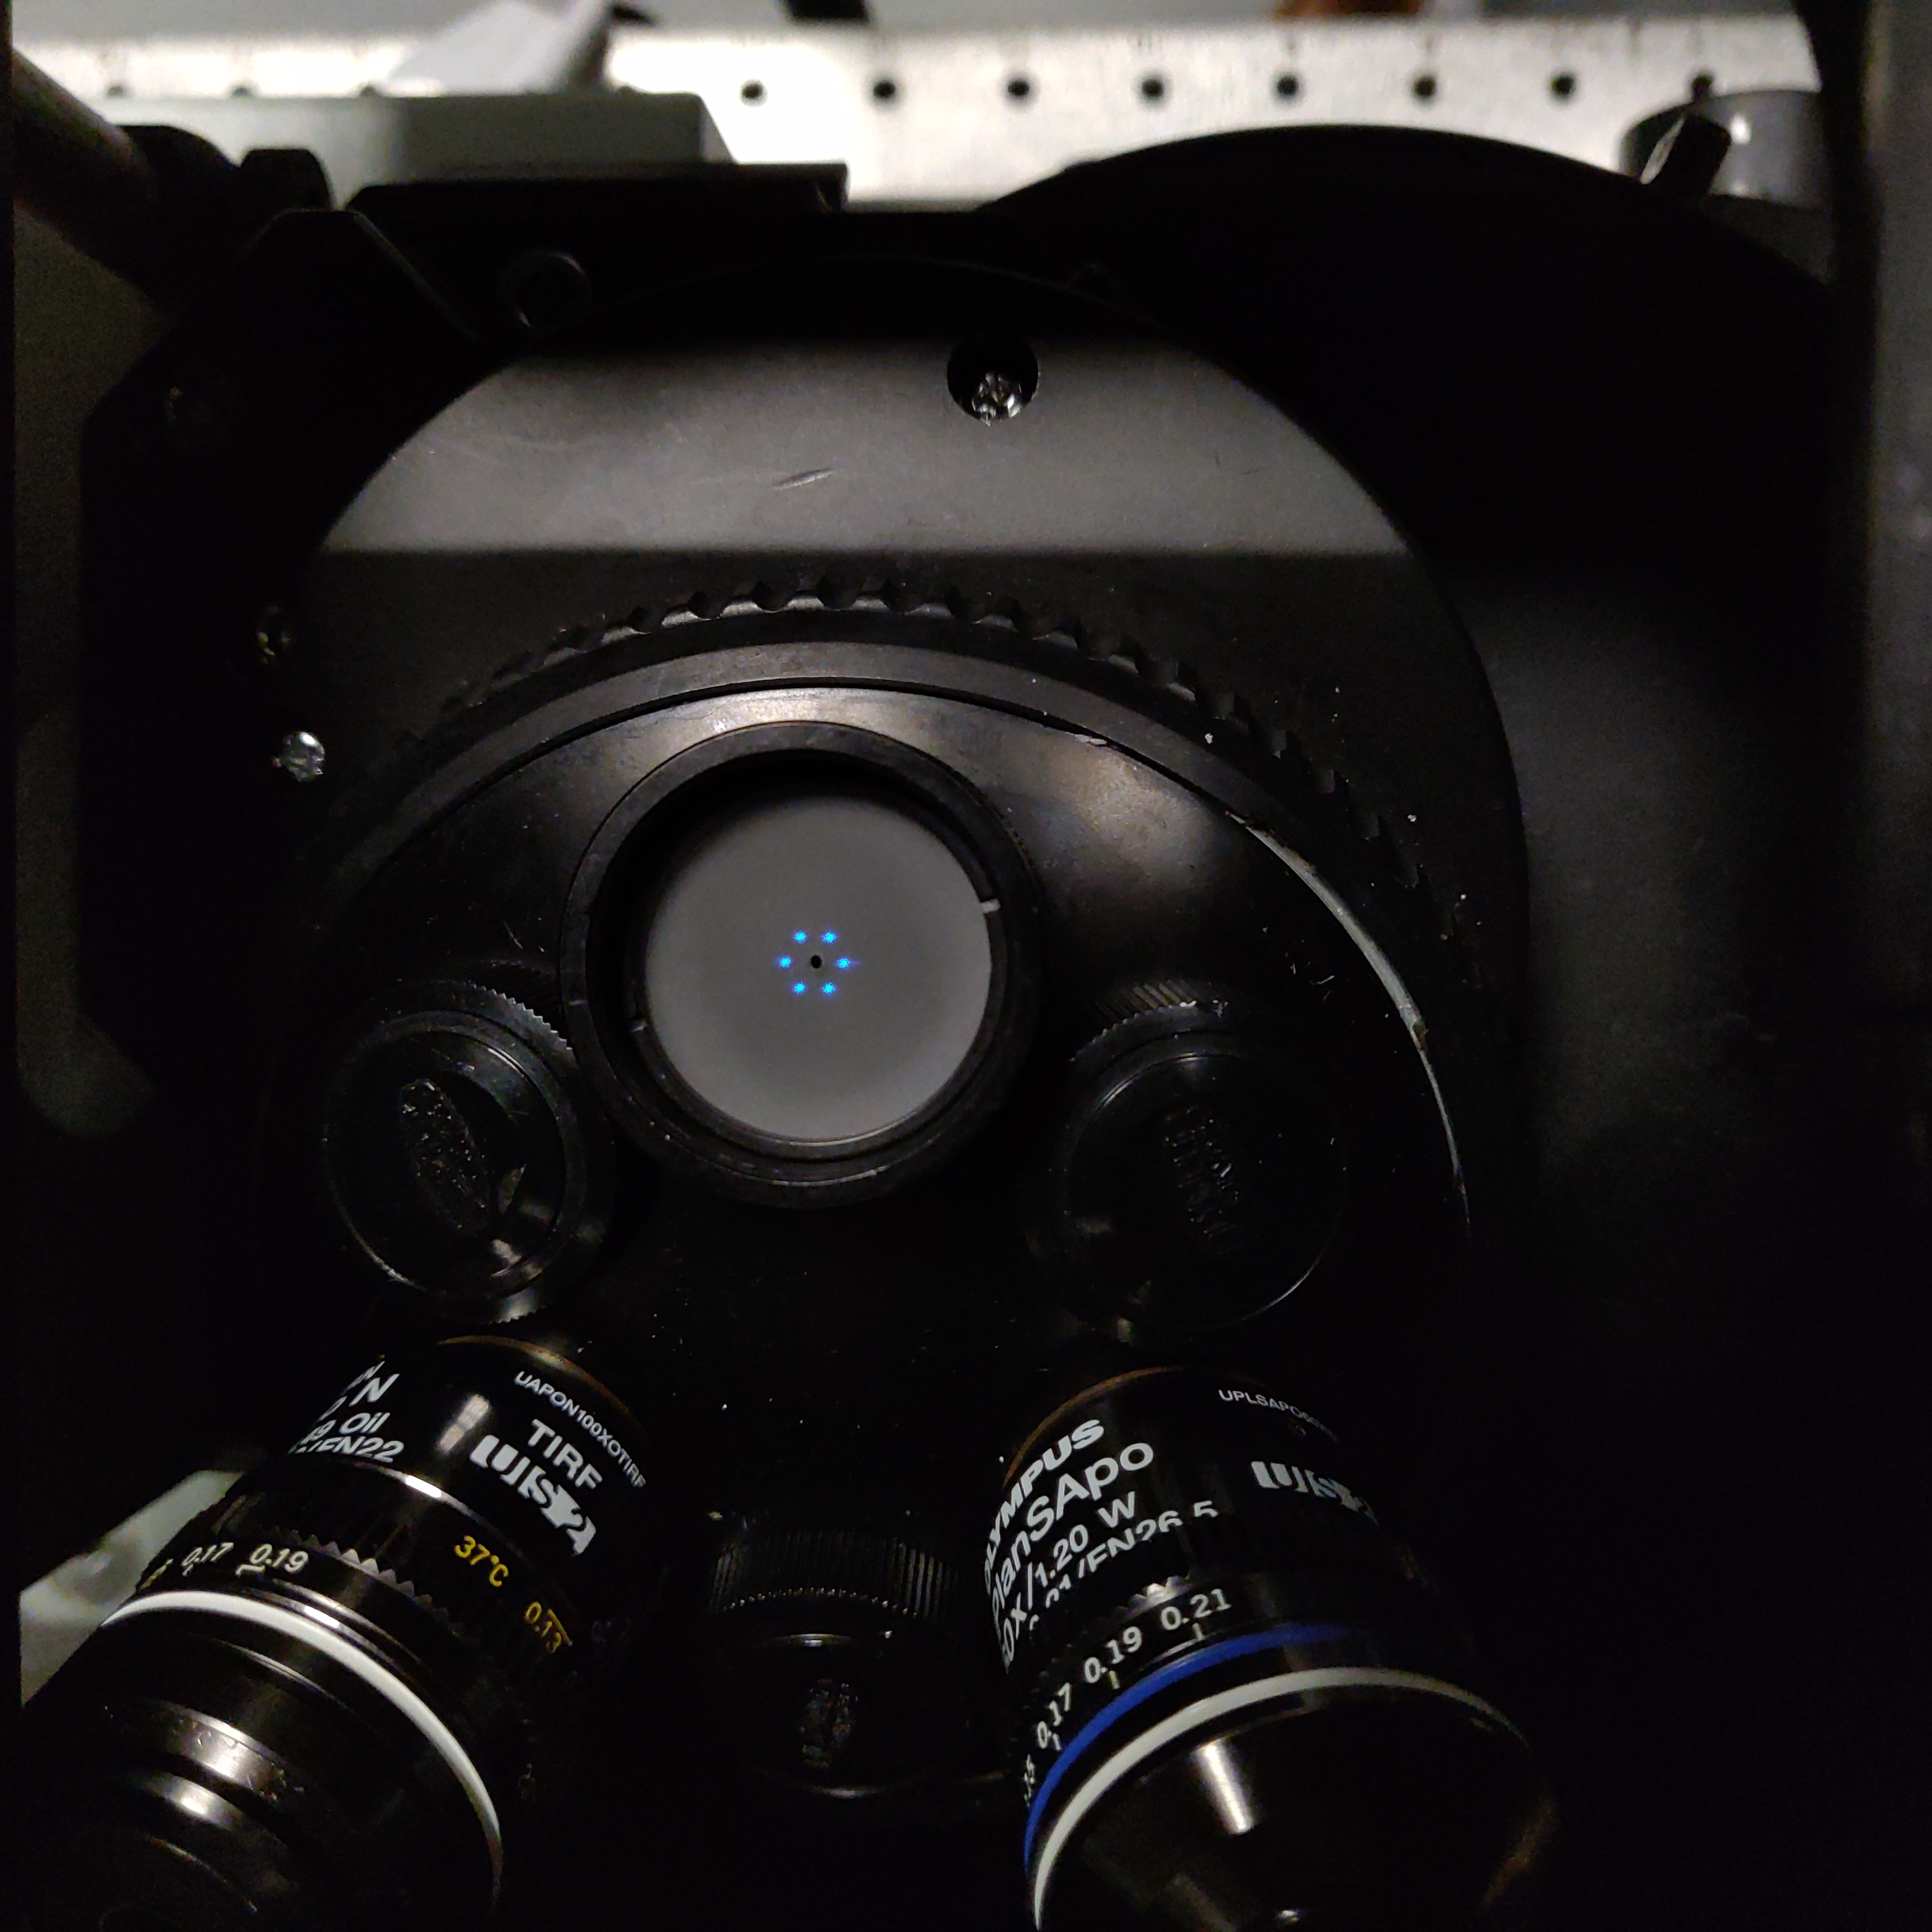
\includegraphics[angle=-90, width=0.6\textwidth]{sim-alignment}
\caption[LAG SIM: Displaying specially designed patterns on the SLM assists with alignment of LAG SIM]{The 3 orientations of the SIM pattern are overlaid on the SLM, such that 6 spots are produced in the Fourier plane for alignment. The spots should be aligned such that the pinhole is at the centre of the spots.}
\label{fig:pinhole-alignment}
\end{figure}

Finally, the \texttt{Piezo Offset} section adjusts the z-position of the stage for each channel to account for chromatic offset. 
In practice this offset is less than \SI{100}{\nano\meter} and \texttt{Piezo Offset} is only used for maintaining correct focus in TIRF imaging. 

\subsection{Log tab provides access to an online logbook}
The LAG SIM control software logs all activity automatically to Labstep, an online laboratory management system~\cite{labstep} shown in Figure~\ref{fig:labstepTimeline}. 

When a user opens the LAG SIM software, they are asked to enter their name for the online logbook. 
When they press \texttt{Start}, the software sends an HTTP request to a Labstep timeline,  recording the user's name and the start time. 
Similarly, when they \texttt{Stop \& Close} the software, their name and finish time is logged to the timeline, along with any errors generated by the software during their use. 

Furthermore, every acquisition is also logged to the timeline. 
This contains metadata relating to the acquisition, for example number of \texttt{t-frames}, \texttt{z-steps}, laser powers, and exposure times. 
This is especially helpful is the user is later unsure what acquisition parameters were used for a particular image. 

The user can also add a customised post to the logbook, for example to record an error with the software. 
The online Labstep logbook can be opened by clicking the \texttt{Open logbook} button, opening the webpage shown in Figure~\ref{fig:labstepTimeline}. 

\begin{sidewaysfigure}[p]
\centering
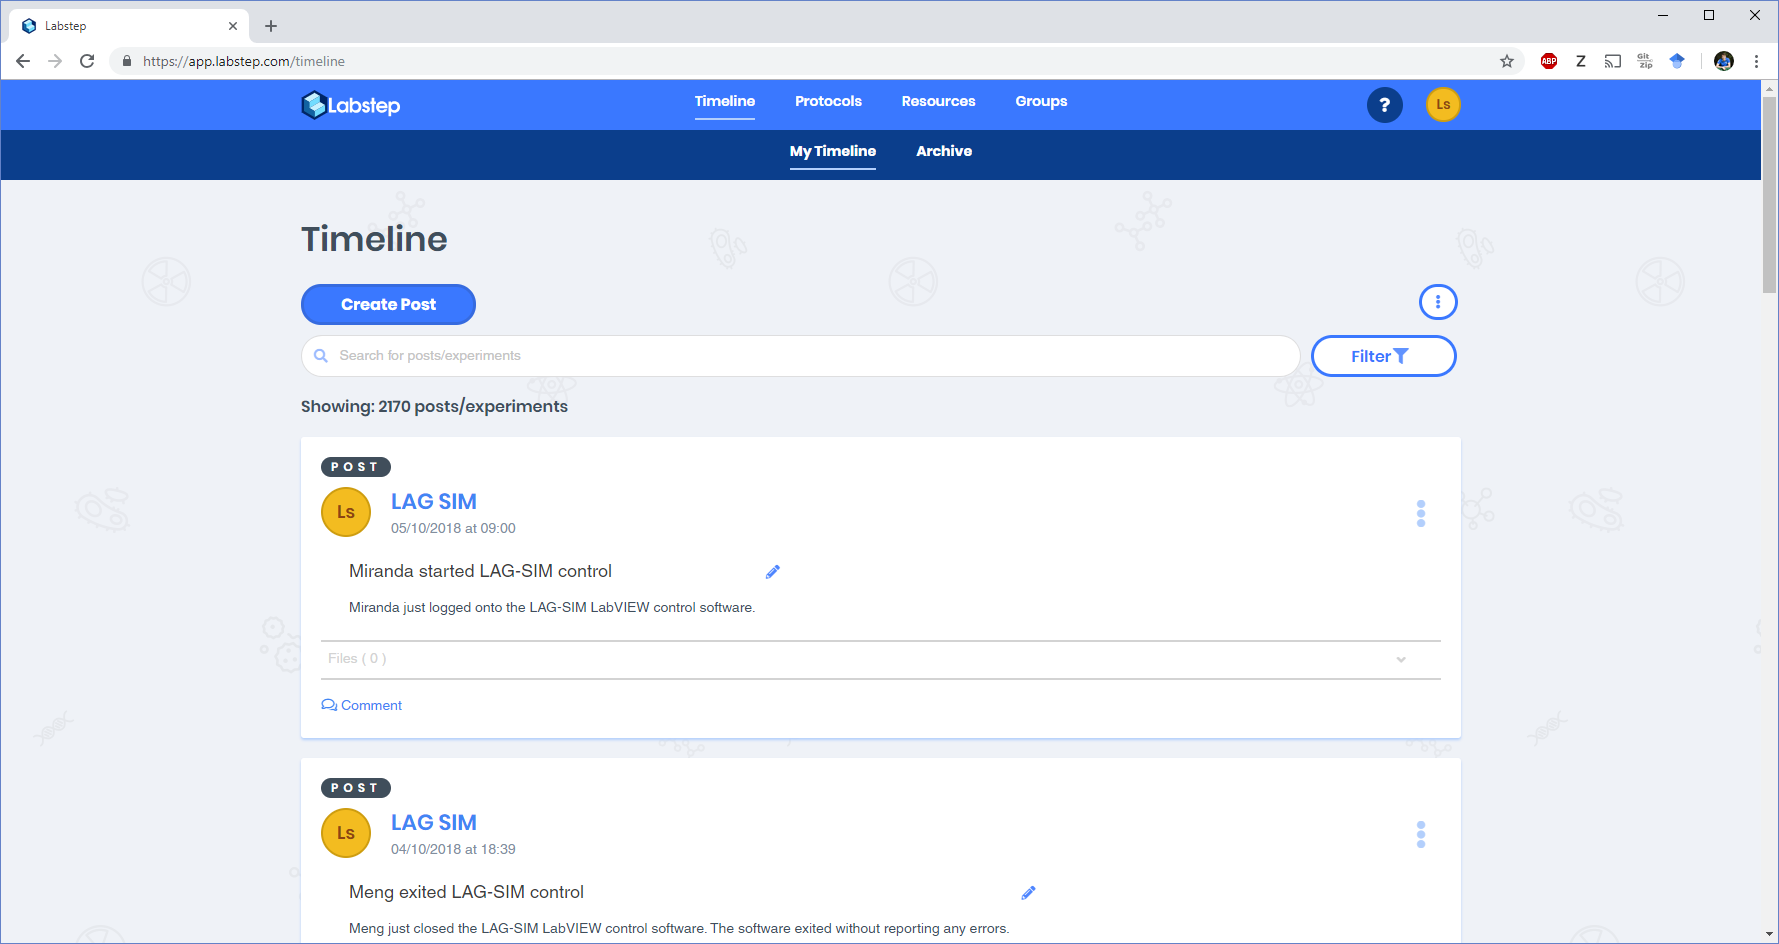
\includegraphics[width=0.875\textwidth]{labstep-timeline}
\caption[LAG SIM: Logging user activity with Labstep allows any problems to be identified and fixed quickly]{User activity is automatically logged to an online logbook hosted on Labstep to identify and fix any problems quickly. This figure shows the user logged onto the SIM at 09:00, acquired 2 images - a SIM z-stack then a 1000-frame widefield video - then logged off.}
\label{fig:labstepTimeline}
\end{sidewaysfigure}

Online logging benefits both the microscope user and the developer, allowing problems to be identified and fixed promptly. 


\section{A comparison of reconstruction algorithms reveals their pros and cons} \label{sec:recon}
Once SIM data is collected, it requires reconstruction to either enhance the resolution, remove out-of-focus light, or a mixture of both.

A basic SIM reconstruction algorithm implements the following steps:
\begin{enumerate}
	\item Extract illumination pattern parameters (orientation angle and phase shift)
	\item Separate Fourier space images into individual frequency components
	\item \label{step:filterPreShift}Weight components in Fourier space by OTF and filter for noise removal
	\item \label{step:shiftComponents}Shift frequency components into correct position in Fourier space
	\item Perform inverse Fourier transform to obtain the reconstructed image
\end{enumerate}

Additional steps are often added into the basic algorithm to reduce artefacts. 
Raw images may be corrected for consistent intensity and contrast across the dataset, and an additional filtering step for noise removal can be applied before the images are separated in Fourier space. 
Note also that step \ref{step:filterPreShift} can be performed after step \ref{step:shiftComponents}, but this can lead to additional artefacts in the reconstructed image~\cite{gustafsson2008three}. 
Artefacts can furthermore be suppressed by apodisation before the final inverse Fourier transform~\cite{gustafsson2008three}. 

This basic algorithm will provide resolution enhancement, but does not implement optical sectioning for removing out-of-focus light.
This requires an additional attenuation step, applied simultaneously with step \ref{step:filterPreShift}. 

Various implementations of the SIM reconstruction algorithm exist.
During the course of my PhD, I have utilised and modified three different reconstruction algorithms, and written a plugin for FIJI tailored specifically for LAG SIM and detailed in Section~\ref{sec:lagsimFiji}.
Each implementation has its own merits and disadvantages, discussed in the remainder of this section.

\subsection{Lin Shao SIM reconstruction runs on CUDA GPUs}
The first implementation of the resolution-enhancing SIM algorithm used in the Laser Analytics Group was provided by Lin Shao, who worked on SIM with Mats Gustafsson~\cite{shao2011super}.
It was developed during his time at Janelia Farm Research Campus, under the supervision of Gustafsson and Eric Betzig~\cite{beach2014nonmuscle}.

Shao's algorithm is written in native CUDA code, a programming model for parallel computation with Nvidia graphics cards~\cite{sanders2010cuda}.
This makes reconstruction very fast - around 1 frame per second on an Nvidia Quadro 2000. 
However, native CUDA must be recompiled from source on every new computer it is used on, and furthermore because the software has not been updated, it does not work with the latest version of CUDA. 

The program has no graphical user interface, but is called from the command line. 
Command line calls can be made from most other programming languages, so a custom interface was built in MATLAB to make reconstruction a simpler process.  
The MATLAB interface firstly separated complex datasets such as multi-channel z-stacks into individual SIM frames, and sent these along with the correct reconstruction parameters, based on the lens used, to the command line reconstruction program. 

Shao's algorithm does not implement OTF attenuation, which is used for optical sectioning.
This means it cannot remove out-of-focus light, so is not appropriate for reconstructing 3D image stacks. 

The program was not built for widespread distribution, and as such there is no documentation or publication for it. 
Nor is the program publicly available; requests for a copy of the software have to be made directly to Lin Shao. 
This means the software is complicated to use, and has not been tested and verified by the wider community. 

Lin Shao is now at Yale University; although he is contactable, he is not actively maintaining this piece of software.
Since this implementation is fast becoming obsolete, it is now only installed on one computer in the Laser Analytics Group, which cannot have graphics updates installed. 

\subsection{SROS-SIM facilitates optical sectioning}
SROS-SIM is a SIM reconstruction program by Florian Str{\"o}hl which implements both optical sectioning and resolution enhancement. 

SROS-SIM is a MATLAB implementation of the super-resolution optical-sectioning (SROS) algorithm detailed by O'Holleran and Shaw in 2014~\cite{oholleran2014optimized}. 
Optical sectioning removes out-of-focus light, so that 3D images can be reconstructed, for example of a whole cell with mitochondria labelled.

As a set of MATLAB scripts and functions, the code can be executed on any computer with a MATLAB license.
Therefore the implementation is available for all major desktop operating systems, and furthermore is easy to modify.
I have made modifications to the original code to perform operations on the graphics processing unit (GPU), bringing a 20$\times$ increase in reconstruction speed. 
% Want to show a table of this??

SROS-SIM has the disadvantage of not being publicly available or published and verified by the community.
Furthermore the need for an expensive MATLAB license limits who can use the software. 
Finally, the important step of measuring the illumination pattern parameters is not fully automated, so that the software always requires some user input and can cannot be left to run unsupervised for a batch reconstruction task.

\subsection{fairSIM allows reconstruction in ImageJ}
fairSIM is an open-source plugin for ImageJ/Fiji, a popular image analysis suite which is also open source and free~\cite{muller2016open}. 
The software is well-documented and hosted on Github, so it is continually updated and improved by the community. 

The fairSIM reconstruction algorithm implements resolution enhancement and optical sectioning, with two different noise filters. 
It provides the user with complete control over the input parameters, and with debugging options enabled will show detailed visual output at each stage of the reconstruction. 
Although the number of options can be overwhelming for some users, it is powerful and useful software for advanced SIM users. 

The fairSIM user interface is cumbersome, and reconstruction can only be performed on a single-colour, single-frame SIM image. 
This process requires around 20 clicks, and input parameters must be resubmitted for every reconstruction. 
This, coupled with the fact that fairSIM does not have GPU support, makes reconstruction very slow, especially for large, multi-colour image sets. 

% Hessian SIM? 

\subsection{LAG SIM is specifically designed for our microscope}
LAG SIM is my personal implementation of the SIM reconstruction algorithm, built using the well-documented fairSIM Java library~\cite{fairsimGithub}. 
It is designed specifically for the Laser Analytic Group's SIM, simplifying the interface for non-advanced users, and implements a fast parameter-finding technique.

It is available publicly as an ImageJ/Fiji plugin~\cite{lagsim}.
This means that it is free, open source, and stays up-to-date for all users. 

The next section describes the LAG SIM plugin in detail, providing a detailed resource to anyone reconstructing LAG SIM data in the future.

\section{Reconstruction with LAG SIM for artefact-free images} \label{sec:lagsimFiji}

\subsection{The LAG SIM ImageJ interface simplifies parameter-finding for non-expert users}

Setting SIM reconstruction parameters, particularly for noise filtering and optical sectioning, is a difficult task for new users.
In LAG SIM, which uses the same reconstruction algorithm as fairSIM, there are 3 filter parameters; 2 apodisation parameters; 2 attenuation parameters; and a choice of 2 filters, which can be used in combination. 
This makes a high-dimensional parameter space to optimise over. 
Selecting appropriate values for these parameters requires understanding what each is for; setting optimum values requires experience and expert skill.

LAG SIM provides a number of tools designed to assist with common SIM reconstruction tasks, reducing the time required between acquisition and analysis of the data.
The tools are accessed through the ImageJ menu shown in Figure~\ref{fig:lagsim-fiji-interface}a. 

\begin{figure}[htbp!]
	\centering
		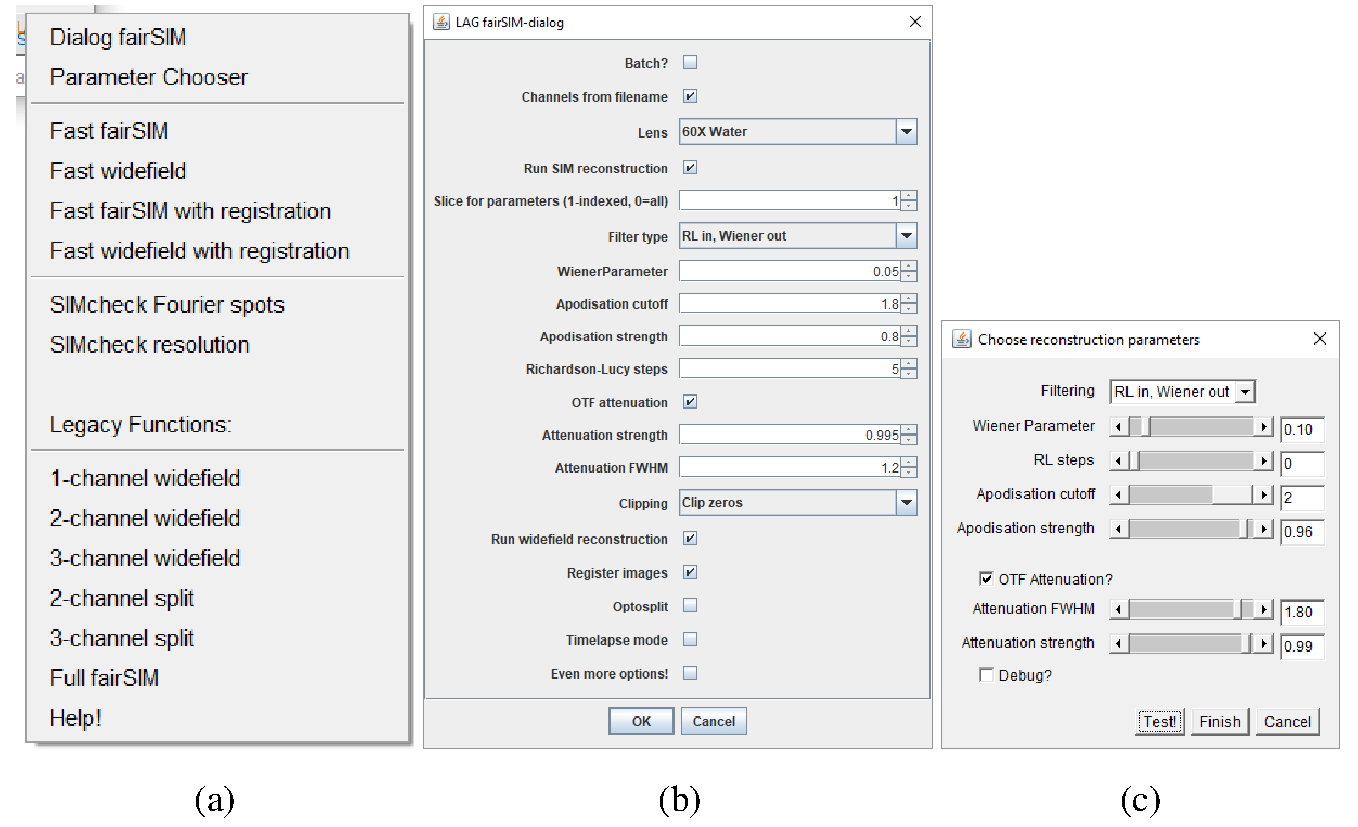
\includegraphics[width=1.0\textwidth]{lagsim-fiji}	
	\caption[LAG SIM: A Fiji interface makes artefact-free reconstruction quick and simple for non-expert users]{The LAG SIM FIJI/ImageJ user interface, utilising the fairSIM reconstruction algorithm, is specifically designed for the LAG SIM to make artefact-free reconstruction quick and straightforward. (a) shows the main LAG SIM menu, with the many reconstruction and SIMcheck tools created; (b) shows the quick parameter tester, for finding the optimal reconstruction parameters; and (c) shows the main reconstruction interface, facilitating batch reconstruction. } 
\label{fig:lagsim-fiji-interface}
\end{figure}

The ``Fast widefield'' function performs a simple pixel-by-pixel sum across the 9 raw images in each SIM acquisition. 
As described in Section~\ref{sec:sim-background}, this simply reconstructs a widefield view of the data.
This is a very fast computational process, and can be used to quickly generate a preview of the data before SIM reconstruction. 
If it later transpires that the acquisition was not good enough for artefact-free reconstruction, for example due to poor signal-to-noise ratio, the widefield reconstruction can be used as a ``better than nothing'' fallback so that the experimental data is not wasted. 
In this way, even in the worst case LAG SIM is as good as a widefield microscope. 

The ``Fast LAG SIM'' function runs a SIM reconstruction on the active ImageJ image with reconstruction parameters which typically produce a good reconstruction, assuming a good signal-to-noise ratio. 
To find more optimal parameters, the ``Parameter chooser'' can be utilised, shown in Figure~\ref{fig:lagsim-fiji-interface}b. 
Every time the ``Test!'' button is pressed, a frame is reconstructed with the given parameters and placed side-by-side with previous test reconstructions.
This allows a user to quickly compare the effect of different reconstruction parameters to produce artefact-free images. 
A detailed description of each parameter follows in Sections~\ref{sec:LAGSIM-illumination-detection} through \ref{sec:LAGSIM-OTF-attenuation}. 

Once appropriate parameters have been chosen for optimal artefact-free reconstruction, the ``LAG SIM dialog,'' shown in Figure~\ref{fig:lagsim-fiji-interface}c is used to reconstruct the full image stack or time series. 
Parameters are saved to the ImageJ user profile, so that they are entered automatically from the parameter chooser and do not have to be entered every time the dialog is opened. 
When the batch checkbox is ticked, a folder-selection dialog window is displayed for reconstructing an entire folder of raw SIM data. 
Progress and estimated finish time are displayed to the user, allowing them to run the task unattended and return later for analysis of the reconstructed data. 

The LAG SIM plugin makes SIM reconstruction a much less time-consuming task than with other reconstruction algorithms, and the convenient ``Parameter chooser'' enables non-expert users to create artefact-free SIM reconstructions. 


\subsection{Illumination detection provides user feedback about pattern modulation contrast}\label{sec:LAGSIM-illumination-detection}
In order to produce an artefact-free reconstruction, the SIM algorithm requires measurement of the illumination pattern to a sub-pixel accuracy~\cite{muller2016open}. 
This is necessary for correctly performing the Fourier-space shift detailed in Section~\ref{sec:SIM-theory}. 

The LAG SIM reconstruction interface (Figure~\ref{fig:lagsim-fiji-interface}c) allows the user to choose which slice the illumination pattern is measured from. 
For z-stacks, it is best that the most in-focus slice is used, to obtain the most accurate measurement. 
Conversely, for a time-series it is best that slice 1 is used, since it will have the least amount of photobleaching. 

Illumination detection with LAG SIM has been designed to require the least amount of user input necessary. 
The user simply needs to select the objective lens used, and the software will infer the necessary information such as pixel size and numerical aperture. 
Wavelength can be extracted directly from the filename if the file is saved using the correct naming convention. 

\begin{table}[h!]
\caption[LAG SIM: Different combinations of lenses, wavelengths, and SLM grating patterns provide different resolution enhancement factors]{\label{tab:resolution}The table shows the resolution enhancement factors for each combination of lens, laser, and SLM mode available for the LAG SIM. When the 100X lens is used in TIRF mode, the full 2$\times$ resolution improvement can be achieved. Note that the 60X ``tSIM*'' mode uses the same SLM patterns as 100X tSIM, but because the 60X lens is not designed for TIRF this does not create total internal reflection at the coverglass. } 
\centering
\begin{tabular}{|c|c|c|c|c|}
\hline
Lens &	Laser (nm) &	Emission (nm) & SLM Mode & Resolution improvement \\ \hline
60X &	488 &	525 &	SIM &	1.59 \\
60X &	561 &	600 &	SIM &	1.67 \\
60X &	640 &	676 &	SIM &	1.61 \\
60X &	488 &	525 &	tSIM* &	1.78 \\
60X &	640 &	676 &	tSIM* &	1.76 \\
100X &	488 &	525 &	SIM &	1.78 \\
100X &	561 &	600 &	SIM &	1.89 \\
100X &	640 &	676 &	SIM &	1.8 \\
100X &	488 &	525 &	tSIM &	2.04 \\
100X &	640 &	676 &	tSIM &	2.01 \\ \hline
\end{tabular}
\end{table}

After this process, the software provides feedback to the user about how well the parameters were detected, based on the modulation depth and the patterns' delta peak locations in Fourier space.
LAG SIM has well-defined resolution enhancement factors based on the period of the SLM grating patterns, shown in Table~\ref{tab:resolution}. 
The resolution enhancement factor is calculated as $1 + \dfrac{t}{O_r}$, where $O_r$ is the radius of the lens' OTF for the given emission wavelength and $t$ is the spatial frequency of the illumination pattern. 
If the detected pattern parameters do not correspond to the expected resolution enhancement factor for a given lens, wavelength, and SLM mode combination, then a warning is presented to the user. 
 
If the delta peaks' Fourier-space positions are correct but modulation contrast is low ($m$<0.5), the software waits for user confirmation that they wish to continue with the reconstruction, and recommends that they need to capture higher quality SIM images. 
Note that feedback is not provided in batch-reconstruction mode. 

\subsection{Wiener filtering and apodisation reduces noise, but can introduce artefacts}
When the Wiener filtering scheme is used for noise removal, the Wiener parameter and apodisation parameters are used in a complementary fashion. 

Noise filtering is particularly important in SIM due to the unnatural relationship between signal-to-noise ratio and spatial frequency caused by Fourier-space shifting. 
A conventional 2D microscope OTF has a peak at 0, and decreases symmetrically, as shown in the widefield Fourier plot in Figure~\ref{fig:wiener-parameter}. 
As noise is assumed to be constant over all spatial frequencies, this causes a decrease in signal-to-noise ratio at high spatial frequencies. 
In SIM, a super-resolution image is built up by shifting the OTF in Fourier space. 
This results in local maxima in signal-to-noise ratio, which can be seen when a low value is chosen for the Wiener parameter. 
The extra noise in this region causes swirling hexagonal noise patterns, seen in the contrast-enhanced reconstruction for $w=0.01$. 

Although these patterns are simply how noise presents in a SIM image, they can easily be misinterpreted as features. 
The Wiener filter is a conventional noise filter used in image processing~\cite[\textit{ch. 4}]{brown2012introduction}, which successfully removes hexagonal SIM noise as shown in Figure~\ref{fig:wiener-parameter} for $w=1.0$. 
The amount of noise filtering can be controlled by the user through LAG SIM's `Wiener parameter' input. 


\begin{figure}[p]
\centering
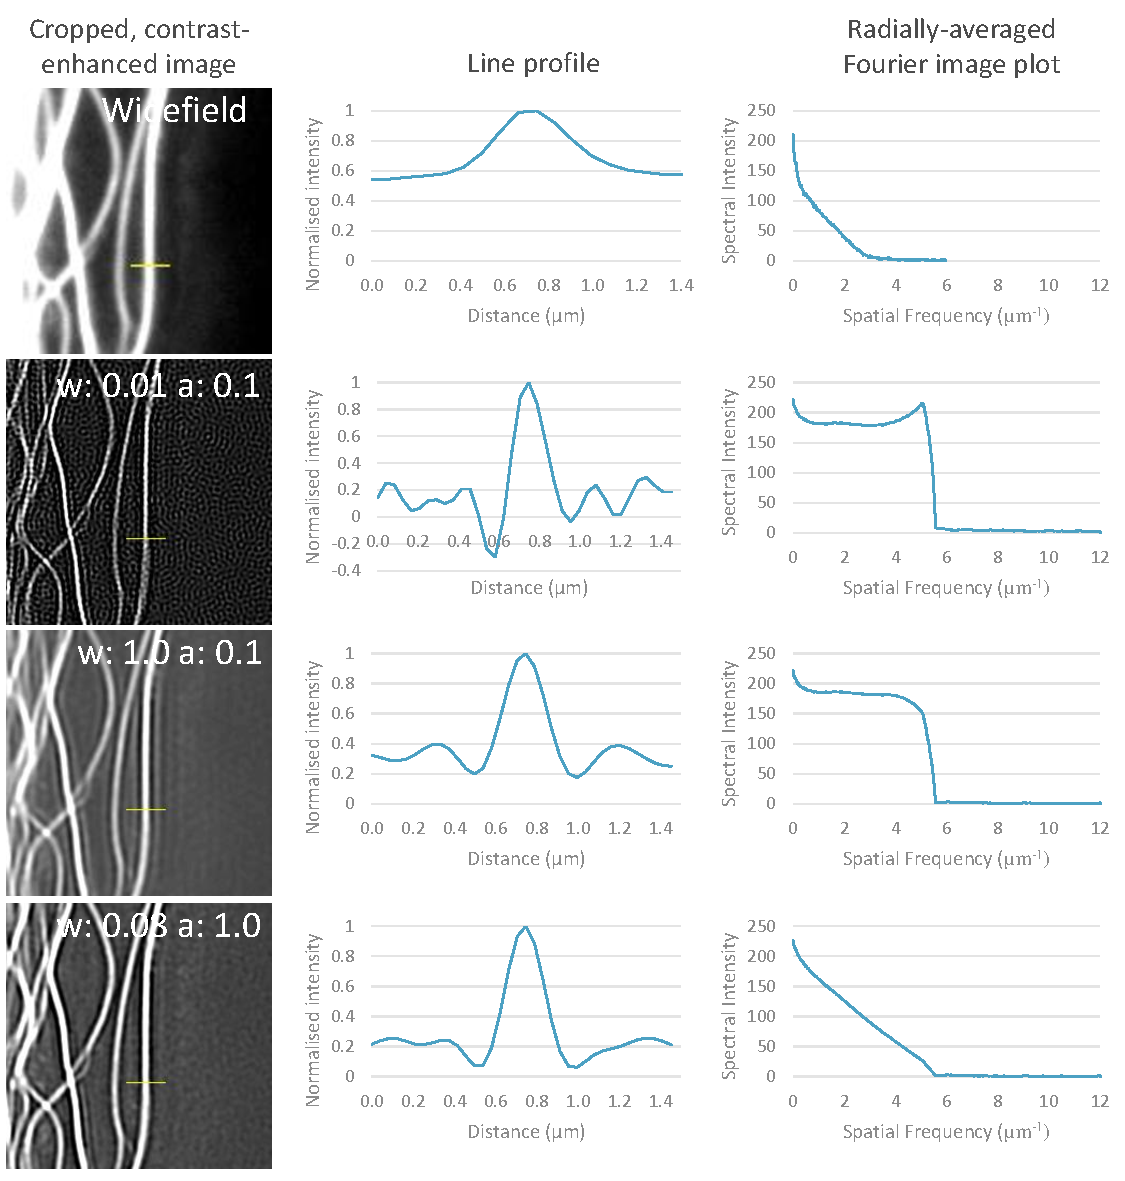
\includegraphics[width=1.0\textwidth]{wiener-parameter}
\caption[LAG SIM: The Wiener parameter and apodisation strength must be chosen to minimise artefacts]{The left column shows crops from a SIM reconstruction with various values of Wiener parameter ($w$) and apodisation strength ($a$), and a widefield image for comparison. Note that image contrast has been greatly enhanced to make the noise pattern visible. The middle column shows the line profile through a tubule, showing the noise pattern with a low Wiener parameter, ringing with a high Wiener parameter, and suppression of noise and ringing using apodisation. The right hand column shows the radially averaged Fourier transform plot of each image; note the local peak when a low Wiener filter is used, which boosts noise at this frequency causing the unconventional noise pattern.}
% Really need to add a, b, c, etc to this, I think. 
\label{fig:wiener-parameter}
\end{figure}

Aggressive noise removal, using high values for the Wiener parameter, can cause ringing in the reconstructed images, clearly visible as side-lobes around the $w=1.0$ reconstruction in Figure~\ref{fig:wiener-parameter}~\cite{righolt2013image}. 
To reduce ringing artefacts, the reconstructed image is passed through an apodisation filter. 

Apodisation applies a smooth low-pass filter, gradually reducing power in higher spatial frequencies avoiding a sharp cutoff. 
The radius of the apodising filter in Fourier space is controlled by the `apodisation cutoff' parameter, where a value of 1 corresponds to the cutoff spatial frequency of the objective lens based on its numerical aperture and the emission wavelength of the image. 
The shape of the apodisation filter is controlled by the `apodisation strength' parameter, where a value of 0 gives a tophat filter, $\frac{1}{\sqrt{2}}$ a triangular filter, and larger values further reduce the full-width half maximum. 

The apodisation cutoff should be set to the same value as the resolution enhancement given in Table~\ref{tab:resolution}, with a maximum value of 2.04 for full SIM resolution enhancement. 
Smaller cutoff values reduce the radius of the reconstruction in Fourier space, directly reducing resolution; a value of 1 corresponds to widefield resolution. 
The apodisation strength should be as small as possible whilst still removing ringing artefacts for maximum contrast of high-frequency features.  

\subsection{Richardson-Lucy filtering introduces less artefacts when optical sectioning is not required} \label{sec:RL-filter}
An alternative filtering scheme for noise removal is Richardson-Lucy deconvolution~\cite{perez2016optimal}. 
The Richardson-Lucy filtering scheme has several advantages over Wiener filtering: it guarantees non-negative pixel values, removing the need for an apodisation step; it does not cause ringing in the reconstructed image; and it only requires one parameter to control the level of noise removal, simplifying the reconstruction process for the LAG SIM user~\cite{perez2016optimal, eichstadt2013comparison}.

\begin{figure}[p]
\centering
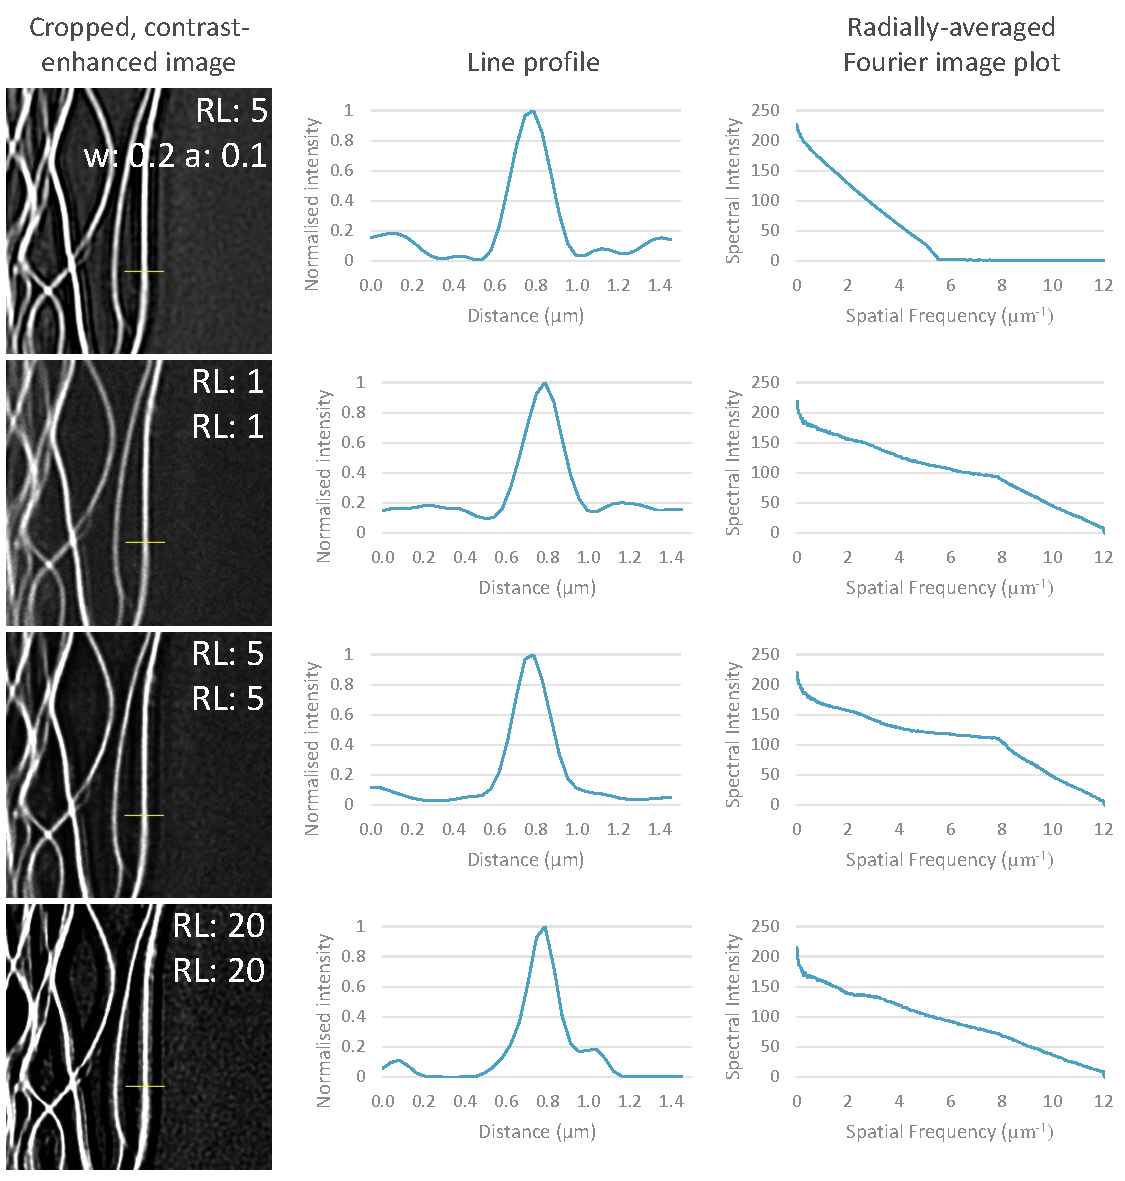
\includegraphics[width=1.0\textwidth]{rl-filtering-figure}
\caption[LAG SIM: Richardson-Lucy filtering can further reduce SIM reconstruction artefacts]{Richardson-Lucy deconvolution on the raw data reduces noise, leading to fewer artefacts in the Weiner-filter reconstruction. Furthermore using Richardson-Lucy filtering for reconstruction produces a more conventionally shaped OTF than Wiener filtering, which further reduces the number of reconstruction artefacts.}
\label{fig:rl-filtering}
\end{figure}

Richardson-Lucy deconvolution is an iterative process, where each iteration of the algorithm converges on the maximum likelihood solution of an image corrupted with Poisson noise~\cite{richardson1972bayesian, lucy1974iterative}. 
The number of iterations is set by the user in LAG SIM.
More iterations result in a narrower point spread function, and thus higher perceived resolution; but can also lead to noise amplification, causing speckle patterns to appear in the reconstructed image.  

Row 1 in Figure~\ref{fig:rl-filtering} shows Richardson-Lucy deconvolution applied to the input images before conventional SIM reconstruction through the Wiener filter. 
This pre-filtering is effective at removing hexagonal SIM artefacts, since less noise is shifted and boosted in Fourier space.

Richardson-Lucy filtering can also be used on the final reconstructed image in place of Wiener filtering. 
Figure~\ref{fig:rl-filtering} shows that as the number of iterations is increased from 1 to 20, bumps in Fourier space caused by SIM reconstruction are smoothed out. 
This narrows the width of the reconstructed line, but can also lead to artificial amplification when the number of iterations is too high. 

Richardson-Lucy input filtering can be used in combination with either the Wiener filter or with more Richardson-Lucy filtering on the reconstructed image. 
Therefore there are in total 4 filtering schemes offered by LAG SIM: Wiener-output; RL-output; RL-input, Wiener-output; and RL-input, RL-output. 

\subsection{OTF attenuation facilitates resolution-enhanced SIM with optical sectioning}\label{sec:LAGSIM-OTF-attenuation}
In conventional widefield microscopy, light from areas above and below the focal plane are captured by the lens, causing out-of-focus light and reducing the axial resolving contrast of the microscope. 
When observing the 3D widefield OTF, shown in red in Figure~\ref{fig:oholleran-otf}, it is clear why this is the case. 
The OTF has no support in the axial direction $z$ at low frequencies, which is known as the `missing cone' problem~\cite{sheppard1992significance}. 

In the Laser Analytics Group's SIM setup, the illumination pattern is only projected onto the sample plane; therefore out-of-focus light does not show the SIM pattern.
Intuitively, one would think this out-of-focus light can be removed by computationally rejecting any part of the image that does not have the SIM pattern, and only showing the in-focus parts of the image with SIM pattern on them. 
O'Holleran and Shaw show that this is achieved practically by attenuating certain parts of the OTF during reconstruction~\cite{oholleran2014optimized}.

If the center part of the OTF is computationally removed, out-of-focus light will be removed from the reconstructed image.
In conventional widefield microscopy, this would have the side-effect of also removing low-frequency information from the image. 
In structured illumination microscopy, however, this information can be recovered from shifted components in Fourier space. 

\begin{figure}[htbp!]
\centering
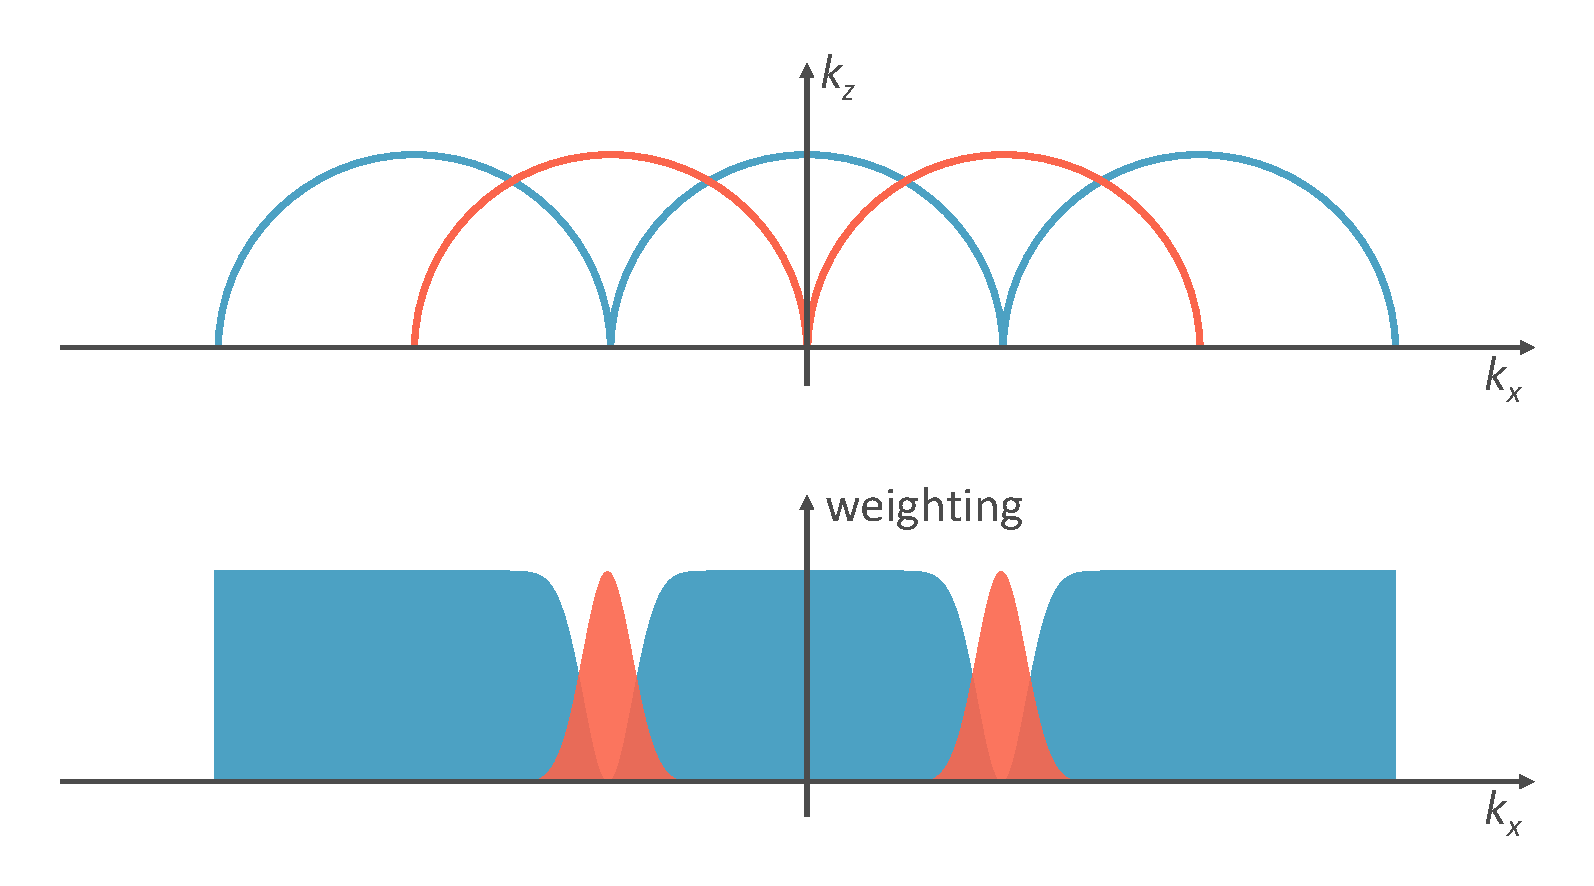
\includegraphics[width=1.0\textwidth]{oholleran-otf-attenuation}
\caption[LAG SIM: OTF attenuation as part of the SIM reconstruction process removes out of focus light]{A widefield OTF, shown in red, does not have axial support at low lateral frequencies, leading to out-of-focus light in widefield images. Applying the red weighting as a Fourier-space filter removes this out-of-focus light; however in conventional epifluorescent microscopy, this would also remove low-frequency spatial information. The Fourier-space shifting inherent to SIM reconstruction recovers the attenuated information, as shown by the blue line, providing support at low lateral frequencies. When the shifted components are filtered by the blue weighting, which removes their own out-of-focus light, an optically-sectioned resolution-enhanced image can be reconstructed.  Adapted from~\cite{oholleran2014optimized}. }
\label{fig:oholleran-otf}
\end{figure}

Figure~\ref{fig:oholleran-otf} shows which parts of the OTF should be attenuated to achieve optical sectioning with no loss of resolution. 
The optical sectioning is controlled by a Gaussian notch in the first-order passbands, shown in blue, and a complementary Gaussian in the zero-order passband, shown in red. 
The width and depth of this passband is controlled in LAG SIM with the parameters `Attenuation FWHM' and `Attenuation strength' respectively.

% Does optical sectioning in this way sacrafice resolution? Well, it sort of depends how far out we push the spots. 
%The water lens is set up for optical sectioning. 

Out-of-focus light makes creating 3D reconstructions impossible. % 3D reconstruction figure
Using optical sectioning to remove this light allows 3D reconstructions of the sample to be created, which can reveal information otherwise unobservable, such as whether a particle is located on the inside or outside of a cell membrane~\cite{teplensky2017temperature}. 

Note that OTF attenuation cannot be used with the Richardson-Lucy output filter. 
Therefore if optical sectioning is required, it is recommended to use the "RL-in, Wiener-out" filtering scheme. 


\section{Results and Discussion} \label{sec:sim-showcase}
LAG SIM has been designed to be a versatile and user-friendly microscope, providing high-speed multi-colour imaging surpassing the diffraction limit with optical sectioning provided computationally or with TIRF. 
With a number of useful automations, LAG SIM can be used to create timelapse videos, 3D reconstructions, large mosaic images, and for unsupervised imaging of multiple cells at different locations around the coverslip. 
As a result, the microscope can and has found applications in a wide variety of biological investigations.

Two such investigations are discussed in detail in Chapters~\ref{chap:MOF} and \ref{chap:ER}. 
This section, however, presents a brief overview of a diverse selection of experiments demonstrating a wide range of LAG SIM's capabilities. 
Acquisition and reconstruction methods are provided as a resource for researchers interested in conducting similar experiments with the microscope. 

\subsection{Multicolour beads for chromatic alignment}
For multicolour SIM experiments, small chromatic offsets between colour channels, shown in Figure~\ref{fig:recon-beads-unaligned}, require that image registration is performed. 
A slide of multicolour sub-diffraction beads can be used for measuring and correcting chromatic offset, because the well-defined points of light have the same spatial distribution in each colour channel. 

For effective registration, the correct density of beads is required, and the beads should be well separated. 
A dense region of beads will form a homogeneous layer across the microscope slide, without well-defined bead coordinates, so cannot be used for registration. 
Conversely if the density of beads is too low then too few beads per field-of-view reduces the accuracy of registration. 

A microscope slide or Labtek\texttrademark\ well with an appropriate density of beads can be prepared as follows: 
\begin{enumerate}
	\item Sonicate \SI{0.1}{\micro\metre} beads for \SI{10}{\minute}
	\item Dilute beads 1:10 in distilled water, producing a \SI{1.8e10}{particles\per\milli\litre} suspension density
	\item Dispense \SI{20}{\micro\litre} of the diluted beads onto a coverglass, or \SI{50}{\micro\litre} into an 8-well Labtek
	\item Wait for the solution to dry, about \SI{2}{\hour}
	\item Add mounting medium: immersion oil for use with the 100$\times$ oil lens, or water for use with the 60$\times$ water lens. 
	\item Mount the coverglass on a glass slide, or replace the lid on the Labtek\texttrademark\ and seal with Parafilm\texttrademark\  to prevent spillages
\end{enumerate}

Following this protocol produces a bead sample with about 100 particles per field-of-view. 
The sonication step means that beads are well spread out, so that individual beads can be accurately localised. 

\begin{figure}[p]
\centering
\begin{subfigure}[b]{0.49\textwidth}
	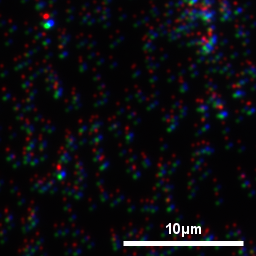
\includegraphics[width=\textwidth]{recon-beads-unaligned}
	\caption{}\label{fig:recon-beads-unaligned}
\end{subfigure}
\hfill
\begin{subfigure}[b]{0.49\textwidth}
	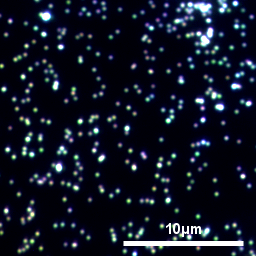
\includegraphics[width=\textwidth]{recon-beads-registered}
	\caption{}\label{fig:recon-beads-registered}
\end{subfigure}
\caption[LAG SIM: Multicolour alignment beads are used for correcting chromatic offset]{A small chromatic offset between the three SIM colour channels can be seen in (a). When the offset is corrected, as in (b), the beads appear white; the offset parameters can then be used to correct other multi-colour images captured during the same imaging session.  } 
\label{fig:recon-beads}
\end{figure}
\afterpage{\clearpage}

Before capturing images, the bead sample can also be used for minimising spherical aberrations introduced by temperature changes and refractive index mismatches. 
When the bead sample is viewed on the microscope, adjusting the correction collar on the objective lens will change the shape of each bead's point-spread function. 
For minimal aberrations, the point-spread function should be symmetrical when defocussing above and below the bead layer. 

To measure chromatic offset, a multi-colour SIM acquisition should be captured in the same colour channels as the subsequent biological experiment. 
The single layer of beads will not have contribution from out-of-focus light, and should also have a high signal-to-noise ratio. 
Therefore the SIM reconstruction process does not require OTF attenuation for optical sectioning, so the Richardson-Lucy filter is recommended on the output stage of the reconstruction process. 
Section~\ref{sec:RL-filter} shows that 5 iterations of filtering reduce noise without introducing artefacts.
The suggested parameters to enter into the LAG SIM Fiji plugin are summarised as follows: \newline
\begin{tabular}{p{0.5\textwidth}}
\begin{labelling}[margin=OTF attenuation]
	\item[Filter] RL out
	\item[RL steps] 5
	\item[OTF attenuation] false
\end{labelling}
\end{tabular}

After reconstruction, there will be some chromatic offset between each channel, as shown in Figure~\ref{fig:recon-beads-unaligned}. 
After registration and correction, Figure~\ref{fig:recon-beads-registered} shows that a red-green-blue (RGB) colour map will produce white beads. 
These same registration parameters can then be used for other multi-colour experiments in the same imaging session. 


\subsection{Resolution-enhanced optical sectioning of HeLa cells shows MOF colocalised with endosomes}
A frequent biological application of microscopy is imaging cultured cells under different treatments or with different genetic modifications~\cite{white1987evaluation, specht2017critical, wang2017analysis}.

Collaborators in the department had been developing a drug delivery system based on metal organic frameworks (MOFs), and wanted to observe the treatment to ensure MOFs were taken up by cells for delivery of their payload. 
In this particular application, which Chapter~\ref{chap:MOF} describes in much greater detail, calcein was loaded into the porous structure of crystalline MOFs as a model drug.
This MOF treatment was incubated with HeLa cells for \SI{24}{\hour}, and uptake over time was captured with microscopy.

Widefield images had shown MOF located at the cell membrane; however widefield's inherent lack of optical sectioning meant that conclusions could not be drawn from these images about whether the MOF was inside or outside the cell~\cite{orellana2015amorphous}.

One microscopy technique often used to provide optical sectioning is confocal imaging; this was unsuitable for this experiment for several reasons. 
Firstly, confocal microscopy has a resolution limit of \SI{200}{\nano\metre}.
The MOF used in this experiment forms crystalline structures on the order of \SI{100}{\nano\metre}, so a higher resolution was required to accurately capture their location. 
Secondly, acquiring a z-stack of confocal images to produce a 3D model of the cell, which is necessary for determining if the MOF is within the cell membrane, is a slow process, with a 3-channel acquisition taking at least \SI{5}{\minute} per cell~\cite{jonkman2015any}.
Since the cells could only survive on the microscope stage for \SI{2}{\hour}, this limited the number of cells which could be captured per imaging session.

The LAG SIM was able to address both these issues. 
It provides optical sectioning with resolution enhancement, resolving the MOFs and accurately determining their location. 
It is also able to capture images faster, requiring just 9 images per plane, rather than point-scanning which takes longer to capture the same amount of florescence emission light~\cite{jonkman2015any}. 

To observe uptake using the laser lines available on the LAG SIM, the following labelling scheme was designed:
calcein, which naturally is fluorescent when illuminated with \SI{488}{\nano\metre} excitation light, was used as the model drug loaded into the MOFs; 
endosomes were labelled with CellLight Early Endosomes-RFP BacMam 2.0; and the nucleus was labelled with HCS NuclearMask™ Deep Red Stain to visualise the cell. 
The LAG SIM's laser lines, \SI{488}{\nano\metre}, \SI{561}{\nano\metre}, and \SI{640}{\nano\metre}, could then be used to excite fluorescence for the MOFs, endosomes, and nucleus respectively. 

Since fast dynamics were not observed, a \SI{200}{\milli\second} exposure time was used per raw frame, to ensure a high signal-to-noise ratio. 
This relatively long exposure time ensured high signal-to-noise ratio.
Similarly, to minimise cross-talk between imaging channels the Optosplit was not employed and filtering was performed by filters in the filter wheel. 

To determine whether MOF had entered the cell or was simply sitting on the cell membrane, it was necessary to view the cells in 3D. 
The 60$\times$ water lens was selected, and operated in optical sectioning SIM mode.  
Images were captured at every \SI{200}{\nano\metre} in the axial direction, to build up a Nyquist-limited z-stack. 

To provide optical sectioning the z-stack was reconstructed in the LAG SIM Fiji plugin with OTF attenuation. 
The full-width half-maximum and depth of the attenuation Gaussian, defined in Section~\ref{sec:LAGSIM-OTF-attenuation}, were set to 1.2 and 0.995 respectively.
These values generally work well to remove out-of-focus light from reconstructed images without introducing artefacts. 

Since OTF attenuation was applied, the Richardson-Lucy filter could not be used on the output stage of the reconstruction; however 5 Richardson-Lucy iterations were applied to the input data to prevent noise-boosting in the reconstruction process, as described in Section~\ref{sec:RL-filter}. 
The Wiener parameter was set to the relatively low value of 0.03 by virtue of the high signal-to-noise ratio of the raw data. 
The apodisation cutoff was set to 1.6 for the \SI{488}{\nano\metre} and \SI{640}{\nano\metre} channels, and 1.67 for the \SI{561}{\nano\metre} channel, since this is the factor of resolution enhancement provided in 60X optical-sectioning SIM, listed in Table~\ref{tab:resolution}. 
Finally the attenuation strength was set to 0.8, to ensure that the OTF of the reconstructed image has the same shape as a conventional OTF, which prevents ringing artefacts. 

The parameters required for the LAG SIM Fiji plugin are summarised as follows:
\newline
\begin{tabular}{p{0.5\textwidth}p{0.5\textwidth}}
\begin{labelling}[margin={Attenuation strength}]
	\item[Filter] RL in, Wiener out
	\item[Wiener parameter] 0.03
	\item[Apodiation cutoff] 1.6
	\item[Apodiation strength] 0.8
\end{labelling} &
\begin{labelling}[margin={Attenuation strength}]
	\item[RL steps] 5
	\item[OTF attenuation] true
	\item[Attenuation FWHM] 1.2
	\item[Attenuation strength] 0.995 
\end{labelling}
\end{tabular} 

\begin{figure}[tbp!]
\centering
\begin{subfigure}[b]{0.7\textwidth}
	\includegraphics[width=\textwidth]{recon-mofcell-2D}
	\caption{}\label{fig:recon-mofcell-2D}
\end{subfigure}

~\newline
\begin{subfigure}[b]{0.7\textwidth}
	\includegraphics[width=\textwidth]{recon-mofcell-3D}
	\caption{}\label{fig:recon-mofcell-3D}
\end{subfigure}
\caption[LAG SIM: 3D SIM reconstruction reveals that MOFs are endocytosed by HeLa cells]{(a) shows a 3-colour SIM reconstruction overlaid on a brightfield image of a cell, with MOF coloured in green, endosomes coloured in magenta and the nucleus coloured in cyan. MOF can be seen located within the cell boundary, and white spots showing colocalisation between green and magenta imply that MOF is taken into cells through an endocytosis pathway. (b) shows another cell with the same colour scheme as a 3D projection, confirming that MOF is truly located within the cell and is not simply sitting on the cell membrane. The 3D data set is available to explore interactively at \mbox{\url{https://fpb.ceb.cam.ac.uk/MOF}}. Cells were prepared for imaging by Michelle Teplensky. Scalebar in (a) is \SI{20}{\micro\metre}. }
\label{fig:recon-mofcell}
\end{figure}
\afterpage{\clearpage}

Figure~\ref{fig:recon-mofcell-2D} shows a 3-colour reconstructed SIM image overlaid on a brightfield image, revealing green MOF particles within the magenta cell boundary. 
Furthermore, white spots in the image show colocalisation between green and magenta, implying that MOF has been taken up into the cell through an endocytosis pathway and is localised within endosomes. 

To confirm that MOF is truly within the cell boundary and is not sitting on top of the cell requires the 3D reconstructions provided by optical sectioning SIM. 
Figure~\ref{fig:recon-mofcell-3D} indeed verifies this.
Whilst some MOF is on the outside of the cell boundary, other fragments of MOF have been endocytosed into the cell. 
White areas of the image again verify MOF colocalised with endosomes. 

The 3D projection shown in Figure~\ref{fig:recon-mofcell-3D} highlights an issue with presenting 3D data on a static 2D medium. 
It is difficult for the reader to understand the orientation and perspective of the data.
For this reason the 3D dataset is also available to explore interactively in a web browser at \url{https://fpb.ceb.cam.ac.uk/MOF}, using the new tool FPBioimage detailed in Chapter~\ref{chap:FPB}. 

This drug-delivery experiment highlights the LAG SIM's capability of imaging live cells in 3D by utilising optical sectioning, and also providing resolution enhancement over other techniques. 
Details of the experiment are presented in Chapter~\ref{chap:MOF}, including timelapse imaging for observing uptake over a \SI{24}{\hour} period, as well as similar experiments delivering therapeutic drugs to cells with different MOFs. 

\subsection{Fast, multicolour imaging of COS-7 cells reveals dynamic colocalisation between ER and lysosomes}
During experiments on the dynamics of endoplasmic reticulum (ER), which are detailed in Chapter~\ref{chap:ER}, we observed a strong interaction between ER and other organelles, including lysosomes and tubulin. 
To develop a deeper understanding of these relationships, we required fast, high-resolution imaging of live cells in multiple colour channels simultaneously. 

To resolve the shape of lysosomes and the fine network structure of ER requires a microscope capable of resolving structures smaller than \SI{100}{\nano\metre}. 
Whilst some super-resolution techniques are able to resolve structures as small as \SI{20}{\nano\metre}, such as STORM and STED, they do not have the imaging speed required to observe fast dynamic events such as ER tubule growth. 
LAG SIM is able to provide resolution beyond \SI{100}{\nano\metre}, at 11\,frames per second, suitable for imaging these organelle dynamics. 

For high resolution, the 100$\times$ oil lens was chosen, although, because we were looking deeper than \SI{100}{\nano\metre} into the cell, it was not operated in TIRF mode. 
To facilitate simultaneous multi-colour imaging, the Optosplit was employed. 
Cross-talk between colour channels was minimised by labelling just two organelles per experiment, in the \SI{488}{\nano\metre} and \SI{640}{\nano\metre} excitation channels. 

\begin{figure}[tbp!]
\centering
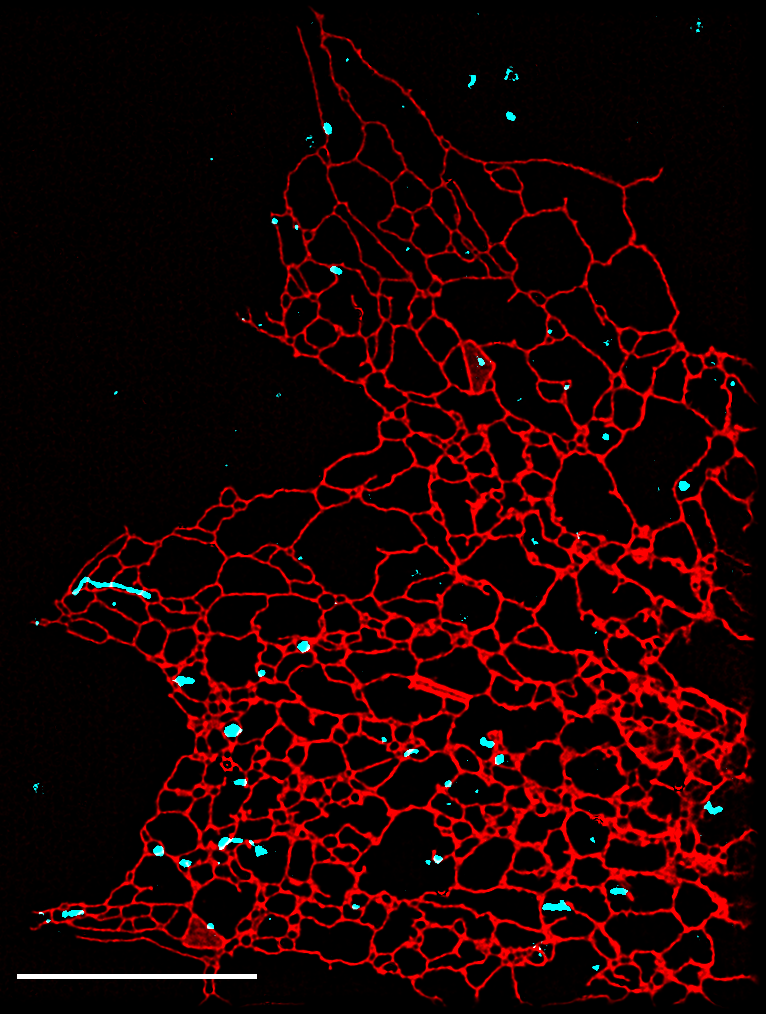
\includegraphics[width=1.0\textwidth]{recon-er-cell}
\caption[LAG SIM: Fast, multi-colour imaging of ER in cells reveals co-localisation between lysosomes and ER tubules]{COS-7 cells with ER is coloured in red, and lysosomes are coloured in cyan. Capturing a timelapse utilising the Optosplit and optical sectioning SIM reveals a dynamic colocalisation between lysosomes and ER tubules, where lysosomes appear to pull the ER network to rearrange connections. Cells were cultured and labelled by Meng Lu. Scalebar is \SI{10}{\micro\metre}. }
\label{fig:recon-er-cell}
\end{figure}
\afterpage{\clearpage}

A time-series of SIM images was acquired at a raw exposure time of \SI{10}{\milli\second} per frame, which equates to a reconstructed image rate of \SI{11}{\hertz}. 
Since optical sectioniong was not required, the Richardson-Lucy filter was used on both the raw images and for the reconstruction output stage, as described in Section~\ref{sec:RL-filter}. 
Richardson-Lucy filtering was performed with 5 iterations, which Figure~\ref{fig:rl-filtering} shows gives a good balance of noise suppression without noise amplification, leading to artefact-free images. 
The parameters required for the LAG SIM Fiji plugin are summarised as follows:
\newline
\begin{tabular}{p{0.5\textwidth}}
\begin{labelling}[margin=OTF attenuation]
	\item[Filter] RL in, RL out
	\item[RL steps] 5
	\item[OTF attenuation] false
\end{labelling}
\end{tabular}

A frame of the reconstructed time series is shown in Figure~\ref{fig:recon-er-cell}, demonstrating artefact-free SIM imaging of ER and lysosomes. 
The figure shows lysosomes in cyan colocalised with ER in red. 
The timelapse video reveals a highly dynamic restructuring of the ER, which appears to be regulated by lysosome movement. 
Lysosomes located on the end of ER branches pull the ER into new shapes, and help attach it to other parts of the organelle to rearrange the network connections. 

Work on these observations is ongoing, with a variety of genetic mutations now being applied to cell lines to understand the biochemistry of these organelle interactions. 

\subsection{TIRF imaging of MEF cells resolves dynamic actin structure on the cell membrane}
Structure on the cell membrane is difficult to observe in epifluorescent microscopy due to out-of-focus light obscuring details in the focal plane. 
This is demonstrated in Figure~\ref{fig:widefield-actin}, a widefield image of mouse embryonic fibroblast (MEF) cells with fluorescently labelled actin coloured in cyan and the protein KRAS in orange. 
Out-of-focus light from areas above the imaging plane make it difficult to distinguish individual actin structures, particularly in areas with a high density of filaments.
The out-of-focus light is even more problematic in the protein channel, producing a bright background blur in the focal plane so that the local distribution of protein cannot be determined. 

As described in Section~\ref{sec:cytoskeleton}, actin is a component of a cell's cytoskeleton, responsible for maintaining the rigid shape of the cell~\cite{alberts2013essential}. 
The KRAS gene and the associated KRAS protein control cell proliferation~\cite{zimmermann2013small} and are involved in the early stages of many signal transduction pathways~\cite{downward2003targeting, kranenburg2005kras}. 
The aim of this experiment was to image the formation and growth of actin in the cell membrane and understand its dependence on the KRAS protein. 

To perform this task required a microscope with TIRF capability to capture fluorescence only from proteins located at the cell membrane. 
Furthermore a resolution beyond the diffraction limit was required to image individual actin filaments in dense areas. 
LAG SIM was chosen for its fast, high-resolution TIRF-SIM capability. 

To image in TIRF at the highest resolution, the 100X  lens was used. 
KRAS protein and actin were labelled with fluorescent probes with emission wavelengths of \SI{488}{\nano\metre} and \SI{640}{\nano\metre} respectively. 
 
To capture the development of a large number of cells over a long time period, LAG SIM's bookmarking feature was used to store the position of cells as described in Section~\ref{sec:lagsimBookmarks}.
This way time lapse imaging of the actin growth could be recorded for many cells.

Out-of-focus light is physically removed by TIRF, so optical sectioning was not required as part of the SIM reconstruction process.
Richardson-Lucy filtering was used on both the input data and in the reconstruction output stage with 5 iterations to remove noise without introducing artefacts, as described in Section~\ref{sec:RL-filter}.
The parameters entered into the LAG SIM Fiji plugin are summarised as follows: \newline 
\begin{tabular}{p{0.5\textwidth}}
\begin{labelling}[margin=OTF attenuation]
	\item[Filter] RL in, RL out
	\item[RL steps] 5
	\item[OTF attenuation] false
\end{labelling}
\end{tabular}

\begin{figure}[tbp!]
\centering
\begin{subfigure}[b]{0.85\textwidth}
	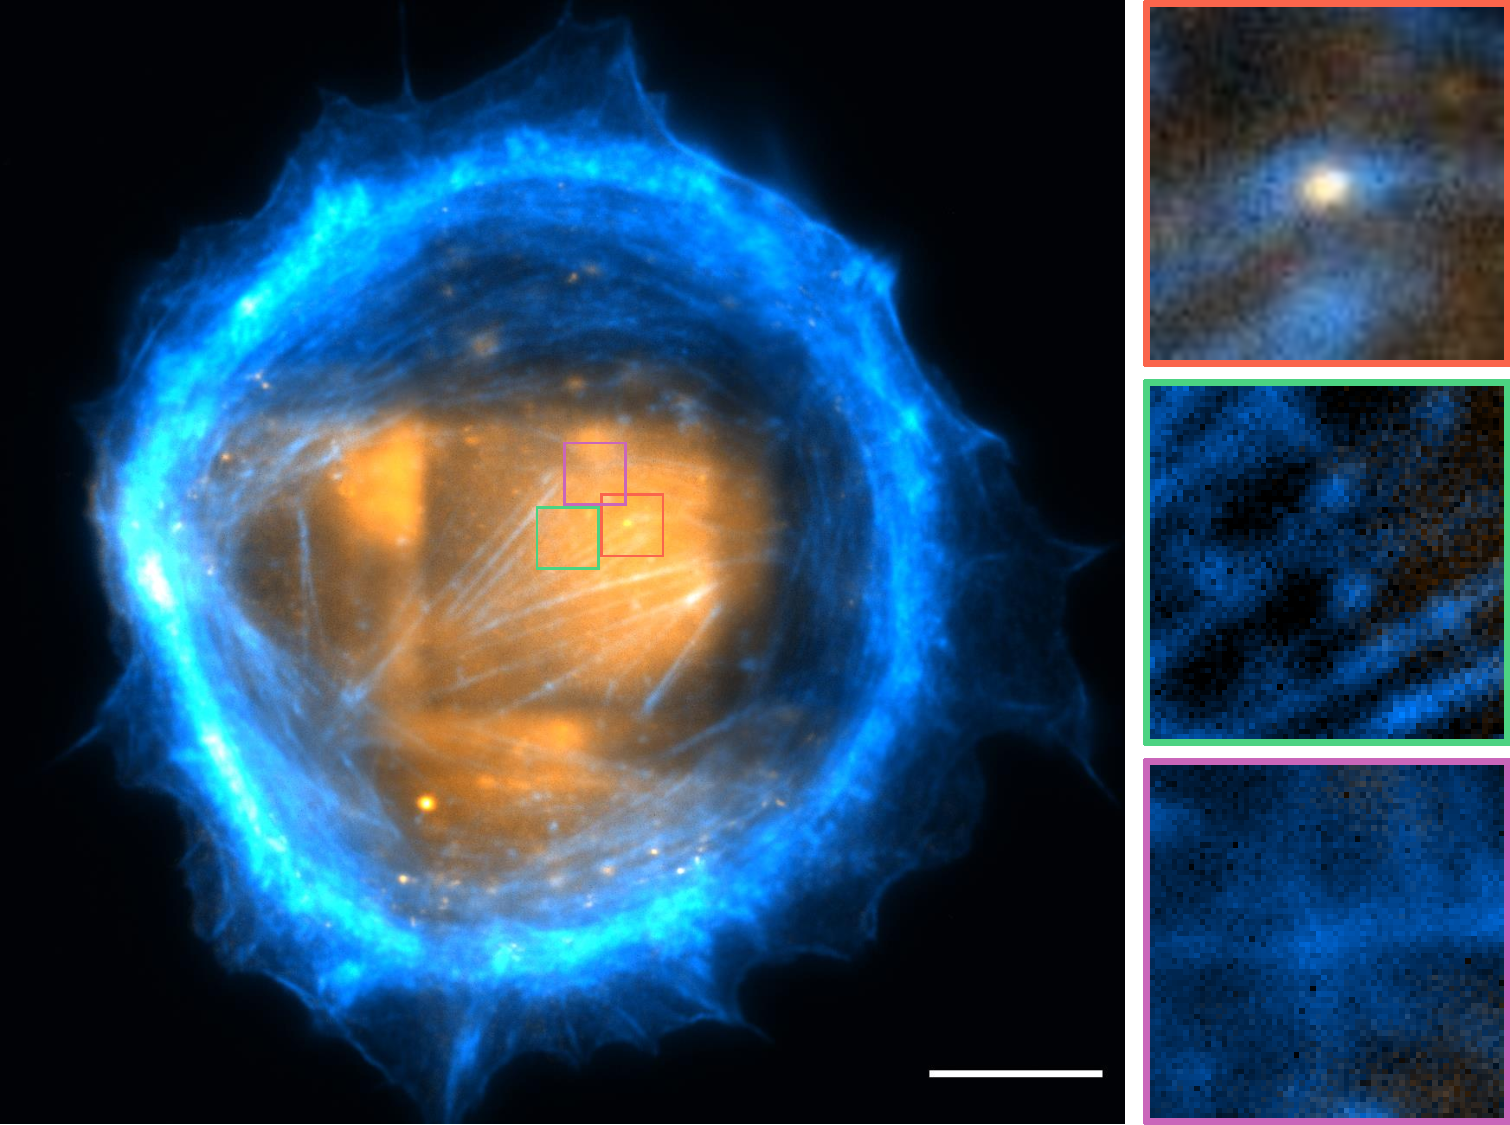
\includegraphics[width=\textwidth]{actin-kras-wf}
	\caption{}\label{fig:widefield-actin}
\end{subfigure}

~\newline
\begin{subfigure}[b]{0.85\textwidth}
	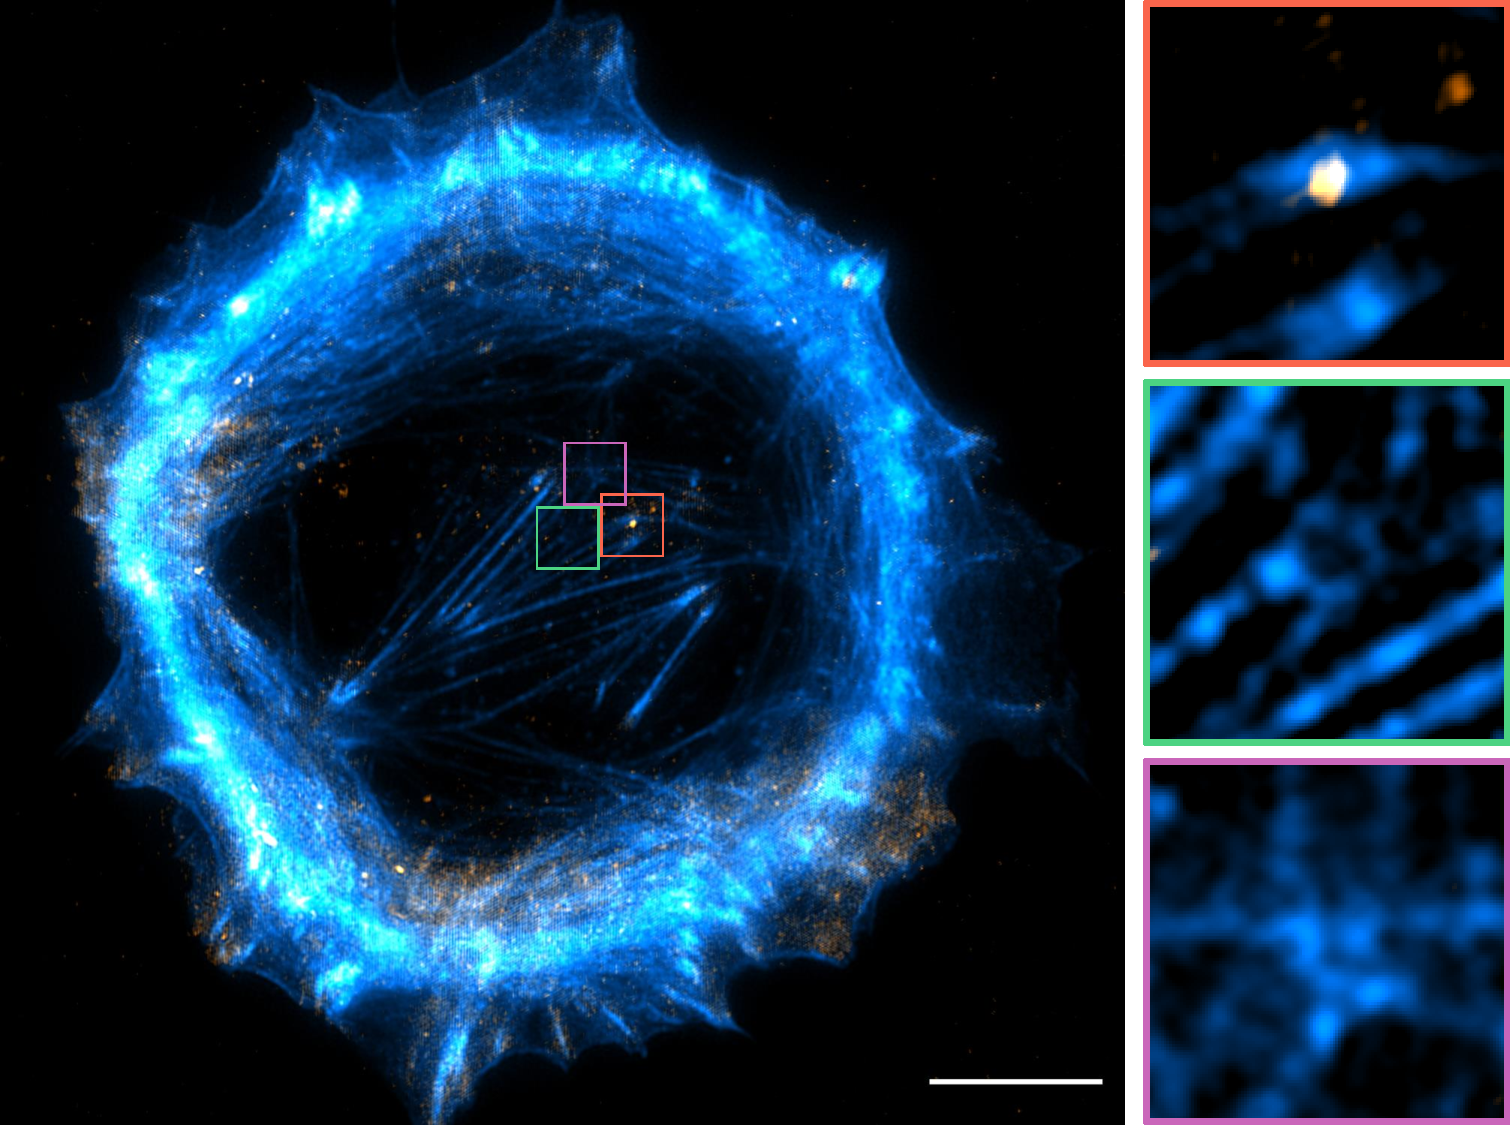
\includegraphics[width=\textwidth]{actin-kras-sim}
	\caption{}\label{fig:recon-tirf-actin}
\end{subfigure}
\caption[LAG SIM: TIRF-SIM imaging of actin in MEF cells removes out-of-focus light allowing actin development to be studied]{(a) shows actin labelled in MEF cells, where out-of-focus light blurs details in the actin. Utilising TIRF-SIM, shown in (b), enhances resolution and removes out-of-focus light. Inset images show various stages of actin development, with a dense cluster of actin (inset in red box) forming into a ring structure (inset in green box) which acts as a source for new filament growth (inset in purple box). Cells were prepared for imaging by Anchal Chandra. Scalebars are \SI{10}{\micro\metre} long, and inset images are \SI{3.2}{\micro\metre} squares.}
\label{fig:recon-actin}
\end{figure}
\afterpage{\clearpage}

A reconstructed TIRF-SIM image is shown in Figure~\ref{fig:recon-tirf-actin}. 
In contrast to the widefield image, individual clusters of protein can now be clearly identified, with the out-of-focus background light removed. 
Furthermore, the structure of individual actin filaments can now be clearly resolved.

During these experiments 3 distinct phases of actin development were observed, shown in Figure~\ref{fig:recon-tirf-actin}'s coloured boxes.
The red box shows an early stage of development, with KRAS protein colocalised with a dense area of the actin label. 
As time progresses, the actin forms a ring structure, seen in the green inset box. 
Finally long actin filaments begin to grow out of the ring structure, as shown in the purple box.

Work is currently ongoing to optimise the labelling of the KRAS protein.
Under the current labelling scheme only one frame of the \SI{488}{\nano\metre} channel could be captured before photobleaching of the fluorescent label reduced the signal-to-noise ratio so that artefact-free SIM reconstruction could no longer be performed. 
Various fluorescent probes are now under investigation to design a scheme where the KRAS protein can be imaged for the full time-lapse duration. 
It is hypothesised that KRAS protein will be colocalised with the ring structure as it forms and as the actin filaments grow from it.
LAG SIM's unique combination of high-speed, high resolution, multi-colour TIRF imaging make it one of the only instruments in the world that can capture these events to test the hypothesis. 


\subsection{Resolution-enhanced optical sectioning of brain-slice tissue imaging for measuring the Node of Ranvier}
Neurons in the brain communicate at junctions known as synapses, which are formed where an axon from one neuron meets a dendrite from another~\cite{hall1992introduction}. 
The axons, coloured yellow in Figure~\ref{fig:neuron-diagram}, form long, thin projections, and can be compared to electrical wires carrying signals across the brain to control bodily functions such as sensing, movement, and conciousness. 

Figure~\ref{fig:neuron-diagram} shows axons coated in a fatty sheath known as myelin~\cite{hall1992introduction}.
This protects the axon from interference with other nearby axons, and increases the transmission speed of electrical signals as action potentials jump from one gap in the myelin sheath - known as a Node of Ranvier - to the next in a process called saltatory conduction~\cite{tasaki1939electro}.
Diseases which cause injury to the myelin sheath are associated with motor neuron disorders such as multiple sclerosis and leukodystrophy~\cite{suzuki2001demyelinating}. 

\begin{figure}[htbp!]
\centering
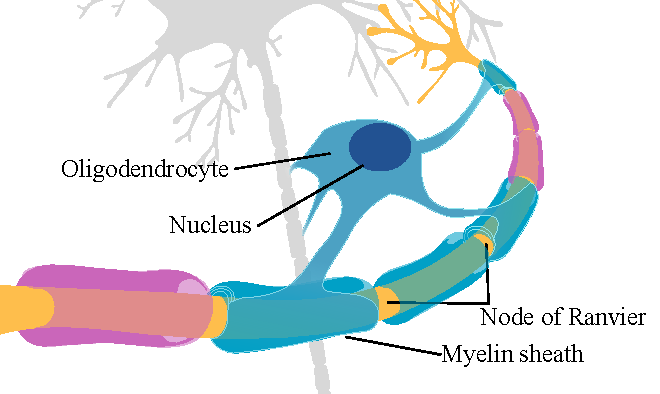
\includegraphics[width=1.0\textwidth]{neuron-diagram}
\caption[LAG SIM: Diagram of a neuron showing an axon protected by the myelin sheath]{Diagram of a neuron, adapted from Wikipedia~\cite{wikineuron}. A neuron, coloured in yellow, has long wire-like projections called axons. Axons are covered by a fatty coating known as the myelin sheath, which protects it from interference from neighbouring axons and increases the transmission speed of signals. The myelin sheath is part of a different brain cell type called an oligodendrocyte, shown here in blue. The gap between two myelin sheaths is known as the Node of Ranvier. }
\label{fig:neuron-diagram}
\end{figure}

The myelin sheath is not part of the neuron cell, but is rather a component of another type of brain cell called an oligodendrocyte, shown in blue in Figure~\ref{fig:neuron-diagram}~\cite{hammond2012cellular}. 
Oligodendrocytes are created from cell-linage parent cells called oligodendrocyte progenitor cells (OPCs), which themselves are derived from embryonic stem cells~\cite{goldman2015make}. 
In mouse models two developmentally distinct OPC populations exist: a first wave of OPCs arise from precursors in the ventral part of the brain at day 15 of embryo development; then a second wave of OPCs from dorsal precursors develop from birth~\cite{kessaris2006competing}. 
Collaborators have shown that when one of these waves of OPCs is genetically suppressed mice are still able to develop to maturity, but have significant difficulties with fine motor control. 

It was hypothesised that a physiological difference in the myelin sheath would be visible between oligodendrocytes derived from ventral OPCs and those derived from dorsal OPCs. 

A fluorescent labelling scheme was devised by collaborators to distinguish between ventrally- and dorsally-derived oligodendrocytes. 
Also, the Node of Ranvier was made visible by labelling the end of myelin sheaths in a third colour; the distance between two adjacent labels was therefore the length of the Node of Ranvier. 
The collaborators were interested to find whether there was a difference in this length for the two oligodendrocyte lineages. 

The SIM examples presented in this results section so far have shown data of cultured cells which form a single layer on the microscope slide, and do not stack on top of each other. 
However, the versatility of LAG SIM also allows it to perform tissue imaging beyond the diffraction limit. 

Imaging deep in tissue is a notorious challenge in microscopy for two main reasons~\cite{wimmer2010high}. 
Firstly multiple layers of fluorescent cells cause significant out-of-focus light, which obscures details in the focal plane.
Secondly, scattering of photons as the light passes through multiple refractive index changes means that it becomes more and more difficult to focus light the deeper into the tissue one tries to observe~\cite{jacques2013optical}. 
Both these issues are particularly problematic in SIM, as the out-of-focus light degrades the modulation contrast of the sinusoidal illumination pattern, and scattering of photons as they travel to the focal plane leads to less pattern-generating interference, as shown in Figure~\ref{fig:tissue-illumination}. 

\begin{figure}[htbp!]
\centering
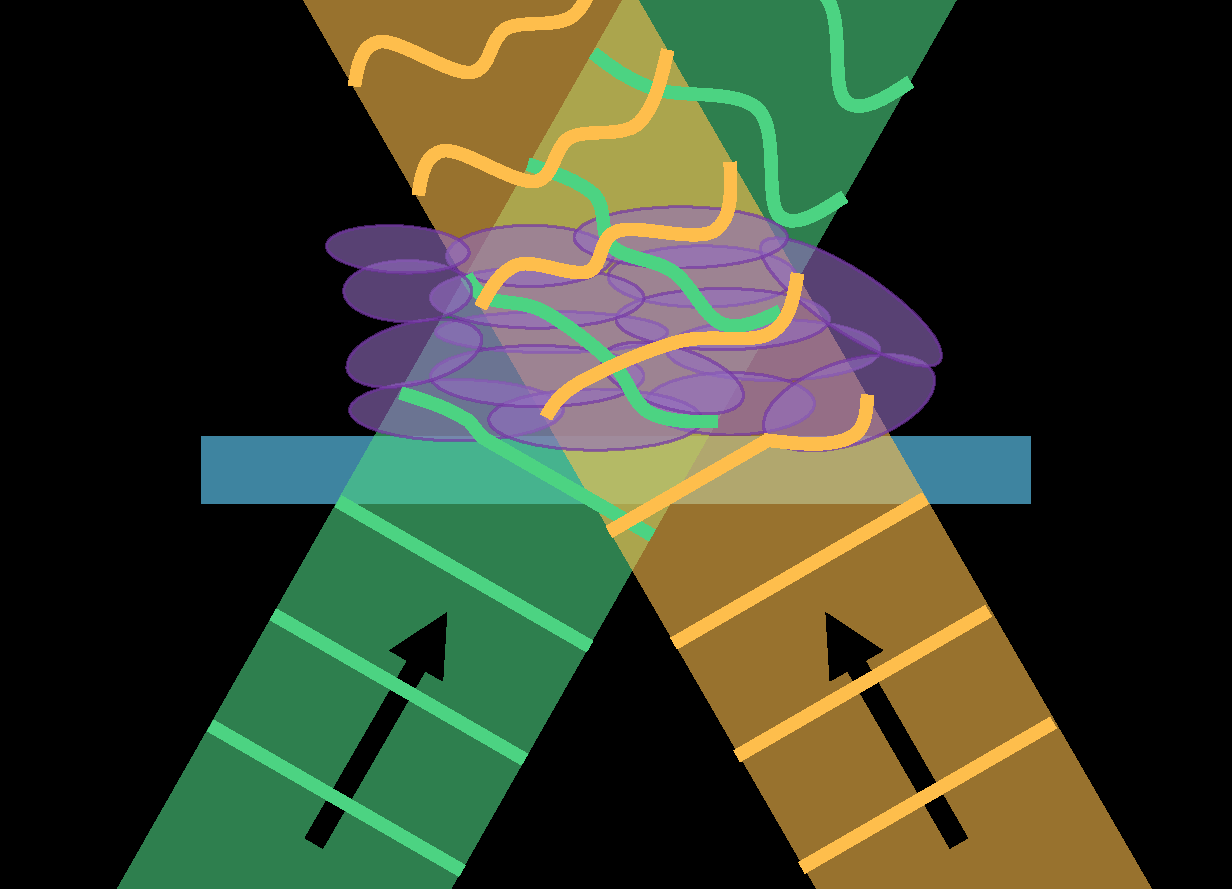
\includegraphics[width=1.0\textwidth]{tissue-illumination}
\caption[LAG SIM: Imaging in tissue degrades the SIM pattern due to photon scattering and out-of-focus light]{A false-colour diagram of SIM imaging in thick tissue samples. 
As light passes through tissue, scattering of photons causes the wavefront to become distorted. When the two beams meet at the focal plane, distortion of the wavefronts means that the sinusoidal interference pattern is degraded. Moreover, out-of-focus light from fluorescence above and below the focal plane further reduces the modulation contrast of the interference pattern. Due to these effects, LAG SIM can only produce reliable images about \SI{10}{\micro\metre} into thick samples. Note that the diagram is not to scale, and that the green and yellow beams come from the same laser source but false-colour has been used for clarity. }
\label{fig:tissue-illumination}
\end{figure}

Nevertheless, it has been found that LAG SIM can image up to \SI{10}{\micro\metre} into tissue without degradation of the reconstructed images. 

\SI{8}{\micro\metre}-thin slices of mouse brain were labelled to study the myelin sheath of oligodendrocytes. 
Myelin was labelled in one of two colours, depending on whether the cell originated from the ventral or dorsal area of the brain. 
The end of each myelin sheath was labelled with a third colour to measure the length of the Node of Ranvier, to discover whether there is an observable difference between the two oligodendrocyte types related to disease pathology. 

To allow the greatest imaging depth, the lens with the closest refractive index matched to the tissue was chosen; in this case, the 60$\times$ water lens. 
A greater penetration depth could be achieved with a lens better matched to the tissue's refractive index, for example a silicon-oil immersion lens with a refractive index of \num{1.406}, if one is available. 
A z-stack was captured with a step-size of \SI{0.2}{\micro\metre}, to build up a 3D image. 
Cells were fixed, so a raw frame exposure time of \SI{200}{\milli\second} was used to ensure a high signal-to-noise ratio. 

To remove out-of-focus light in the reconstructed SIM images, OTF attenuation was used in the LAG SIM Fiji plugin. 
An attenuation FWHM of 1.2 and an attenuation strength of 0.995 were chosen, which Section~\ref{sec:LAGSIM-OTF-attenuation} shows provide optical sectioning without introducing artefacts. 
Richardson-Lucy filtering was applied to the input images to suppress noise, and a Wiener parameter of 0.1 was chosen for output filtering. 
Table~\ref{tab:resolution} shows that the resolution enhancement provided by the 60$\times$ lens in optical sectioning mode is 1.59 to 1.67 - however, relatively weak pattern modulation contrast lead to high-frequency artefacts in reconstructed images, so an apodisation cutoff of 1.5 was chosen to suppress artefacts as much as possible, with an attenuation strength of 0.8 to approximate the shape of a widefield OTF. 

The reconstruction parameters entered into the LAG SIM Fiji plugin are summarised as follows:\newline
\begin{tabular}{p{0.5\textwidth}p{0.5\textwidth}}
\begin{labelling}[margin={Attenuation strength}]
	\item[Filter] RL in, Wiener out
	\item[Wiener parameter] 0.1
	\item[Apodiation cutoff] 1.5
	\item[Apodiation strength] 0.8
\end{labelling} &
\begin{labelling}[margin={Attenuation strength}]
	\item[RL steps] 5
	\item[OTF attenuation] true
	\item[Attenuation FWHM] 1.2
	\item[Attenuation strength] 0.995 
\end{labelling}
\end{tabular}

\begin{figure}[tbp!]
\centering
\includegraphics[width=1.0\textwidth]{recon-brain}
\caption[LAG SIM: Multi-colour optical sectioning SIM to measure the Node of Ranvier on ventrally- and dorsally-derived oligodendrocytes]{Dorsally-derived and ventrally-derived oligodendrocytes are coloured in magenta and cyan respectively. The end of the myelin sheath is coloured in orange, and can be used to measure the length of the Node of Ranvier. Optical sectioning SIM was used on \SI{8}{\micro\metre} brain slices. Slices were dissected and labelled by Sarah F{\"o}rster. Scalebar is \SI{10}{\micro\metre}. }
\label{fig:recon-brain}
\end{figure}
\afterpage{\clearpage}

Figure~\ref{fig:recon-brain} shows a slice of a reconstructed z-stack. 
Orange dots marking the ends of myelin sheaths are located either on dorsally-derived oligodendrocytes, shown in magenta, or on ventrally-derived oligodendrocytes, shown in cyan. 
The length of the Node of Ranvier is measured as the distance between two adjacent orange markers.
Lengths were measured automatically with a custom script in the image analysis suite Icy~\cite{de2012icy}, and assigned to ``dorsally-derived'' or ``ventrally-derived'' based on the colour of the oligodendrocyte they were located on. 

The signal-to-noise ratio in the reconstructed images is notably poor for the oligodendrocyte channels, and artefacts have been introduced by the SIM algorithm despite optimal reconstruction parameters. 
This can be explained by a high 3D density of oligodendrocytes, causing lots of out-of-focus light in the focal plane which reduces the modulation contrast of the SIM illumination pattern. 
As derived in Section~\ref{sec:SIM-theory}, pattern contrast is directly proportional to signal-to-noise ratio for the high-frequency components in reconstructed SIM images, so excessive background light severely affects the ability to produce clear SIM images. 

In contrast to the oligodendrocyte channel, the orange Node of Ranvier channel has a low density of fluorescent markers. 
The SIM pattern modulation contrast is therefore not degraded by out-of-focus light, leading to artefact-free SIM reconstructions with a high signal-to-noise ratio. 
This allows accurate length measurements of the Node of Ranvier. 
Since length was the important measurement for this experiment, and the oligodendrocyte type could still be determined despite the substandard reconstruction, the images were sufficient for testing the hypothesis that dorsally-derived oligodendrocytes have a different Node of Ranvier length from ventrally-derived oligodendrocytes. 

Upon analysis of the data a statistically-significant difference was not calculated, suggesting that there is no difference in the Node of Ranvier length between the two oligodendrocyte types and that the movement problems observed at the organism level must arise from another characteristic of the cells, or a more complicated combination of properties. 
Nevertheless, this experiment has shown the versatility of the LAG SIM instrument and its ability to image tissue samples as well as cultured cells. 

\section{Conclusion}
LAG SIM has been restored to its fast imaging speed of 11 super-resolution frames per second through the introduction of a Pockels cell for polarisation rotation. 
The Pockels cell is a robust, future-proof solution to ensure that the SIM illumination is generated with high pattern contrast. 
With this successfully in place, the other desirable features for LAG SIM could be addressed. 

The instrument can now quickly switch between TIRF imaging, resolution-enhanced SIM imaging and SIM optimised for optical sectioning using user-friendly software which interacts seamlessly with the new hardware. 
This makes it suited to a wide variety of biological imaging experiments, as presented in Section~\ref{sec:sim-showcase}. 

The addition of an Optosplit, made possible by the implementation of the Pockels cell in lieu of an LCVR, further enhances LAG SIM's fast imaging capability. 
Rather than requiring the use of a filter wheel to switch between colour channels, 3 colours can be imaged simultaneously. 
This removes any mechanical movement from the system, reducing the fastest 3-channel acquisition from \SI{570}{\milli\second} to the headline \SI{90}{\milli\second}, a 5-fold improvement in frame rate. 

Considerable care has been taken to ensure the microscope can be operated by non-expert users. 
The interface is clear and compact, and can be taught to new users in a single imaging session. 
This means that LAG SIM can be used unsupervised, saving time and allowing for the microscope to perform a diverse range of world-leading biological research.

Finally, the LAG SIM Fiji plugin complements the easy-to-use microscope to help users generate artefact-free images. 
As shown throughout this chapter, reconstruction is a complicated process involving complex mathematics and optical engineering. 
LAG SIM simplifies this process, so that a user can go from hypothesis to result without the need for a full-time SIM expert. 

In addition to the biological investigations presented here, Chapters~\ref{chap:MOF} and \ref{chap:ER} describe in detail two successful experiments facilitated by LAG SIM. 
Before that, however, Chapter~\ref{chap:FPB} reveals FPBioimage, a user-friendly tool for visualising and sharing 3D volumetric data, such as those obtained through optical sectioning on the LAG SIM. 
%!TEX root = ../thesis.tex
%*******************************************************************************
%****************************** Third Chapter **********************************
%*******************************************************************************
\chapter{FPBioimage: 3D visualisation on the web} \label{chap:FPB}

% Don't forget to PEE/L


% **************************** Define Graphics Path **************************
\ifpdf
    \graphicspath{{Chapter3/Figs/Raster/}{Chapter3/Figs/PDF/}{Chapter3/Figs/}}
\else
    \graphicspath{{Chapter3/Figs/Vector/}{Chapter3/Figs/}}
\fi

``Marcus, hats off; your FPBioimage really rolls.''

\textit{Email from Konrad K\"olble, 20-06-2018}

\section{Introduction}
\subsection{Data Availability} \label{sec:introvisual}
Modern scientific experiments gather data at an ever-increasing rate. 
This is particularly apparent in 3D microscopy, where techniques such as confocal, optical-sectioning SIM, and light-sheet techniques including selective plane illumination microscopy (SPIM) generate terabytes of volumetric data per hour. 

Popular scientific journals require authors to make data available for reproducibility and further analysis. % Perhaps a quote here from one or two journals? 

To give the reader a deeper understanding of 3D data, many authors present it with fly-through videos showing the data from a variety of perspectives, including from within the volume. 
Whilst this provides significantly more information than static 2D images can provide, the reader is nevertheless unable to interact with the data themselves. 
They are therefore restricted to just the perspective provided by the author, with no opportunity for personal exploration or analysis.
To describe the data as open access should require a link to the volumetric data set so that readers can download it and examine it themselves. 

It is perhaps understandable, however, that most published work does not contain links to full volumetric data sets; hosting and maintaining such large volumes of data online incurs prohibitively expensive costs. 
Repositories specifically designed for this type of data are emerging, such as the Image Data Resource (IDR) from OMERO, but have not been widely adopted. 
Many authors therefore simply make a statement that their data is "available upon reasonable request". 

In my experience, authors are very willing to accommodate requests for such data. 
However, receiving and examining 3D volumetric data is not trivial. 
The large file size means that the common practice is to temporarily upload data to a Dropbox file repository, and share a link to the repository through an email. 
Once the large data file has been downloaded, specialist image analysis software must be used to render it, requiring expert skill and experience. 

As a producer of volumetric data, I faced the data sharing issue myself when one of my collaborators moved to Chicago. 
We had gathered 3D data utilising optical sectioning on the SIM, as described in Chapter~\ref{chap:SIM}, which now required their specialist biological interpretation. 
The issue was further complicated since the collaborator had little knowledge of volume rendering software, so could not easily examine the data. 

To solve this, I searched for an online application where I could easily upload 3D data to share immediately with my collaborator. 
Finding that none existed, I created First Person Bioimage (FPBioimage), my own tool to fulfil these requirements.
% The development and implementation of FPBioimage is detailed in this chapter. 

\subsection{Volumetric rendering} \label{sec:volumerendering}
The first demonstration of volumetric rendering was by Pixar in 1987 \cite{smith:1987}, a year after their aquisition from Lucasfilms by Steve Jobs for \$\num{5000000} (a bargin considering it was sold to Disney in 2006 for \$\num{7400000000} \cite{pixarfilm:2007, pixarstory:online}).
For the first time, a full volumetric rendering of a computerised tomography (CT) scan was displayed.

At SIGGRAPH '88 \cite{smith:1988panel} Alvy Ray Smith clarified the difference between between volumetric rendering and traditional, geometric rendering.
In geometric rendering, an object is described by one or more geometrical shapes, such as a collection of spheres and cubes.
To render the object, the surface of the shape is approximated by a mesh of triangular primitives, and the interaction of a virtual light ray with each triangle is calculated.

Volumetric rendering uses a fundamentally different technique.
A virtual light ray begins at a pixel on the screen, and progresses through a 3D array of voxels, as shown in Figure~\ref{fig:raymarchDiagram}.
At equally spaced steps along the ray, the value of the voxel is recorded to build up a ray profile.

\begin{figure}[htbp!]
\centering
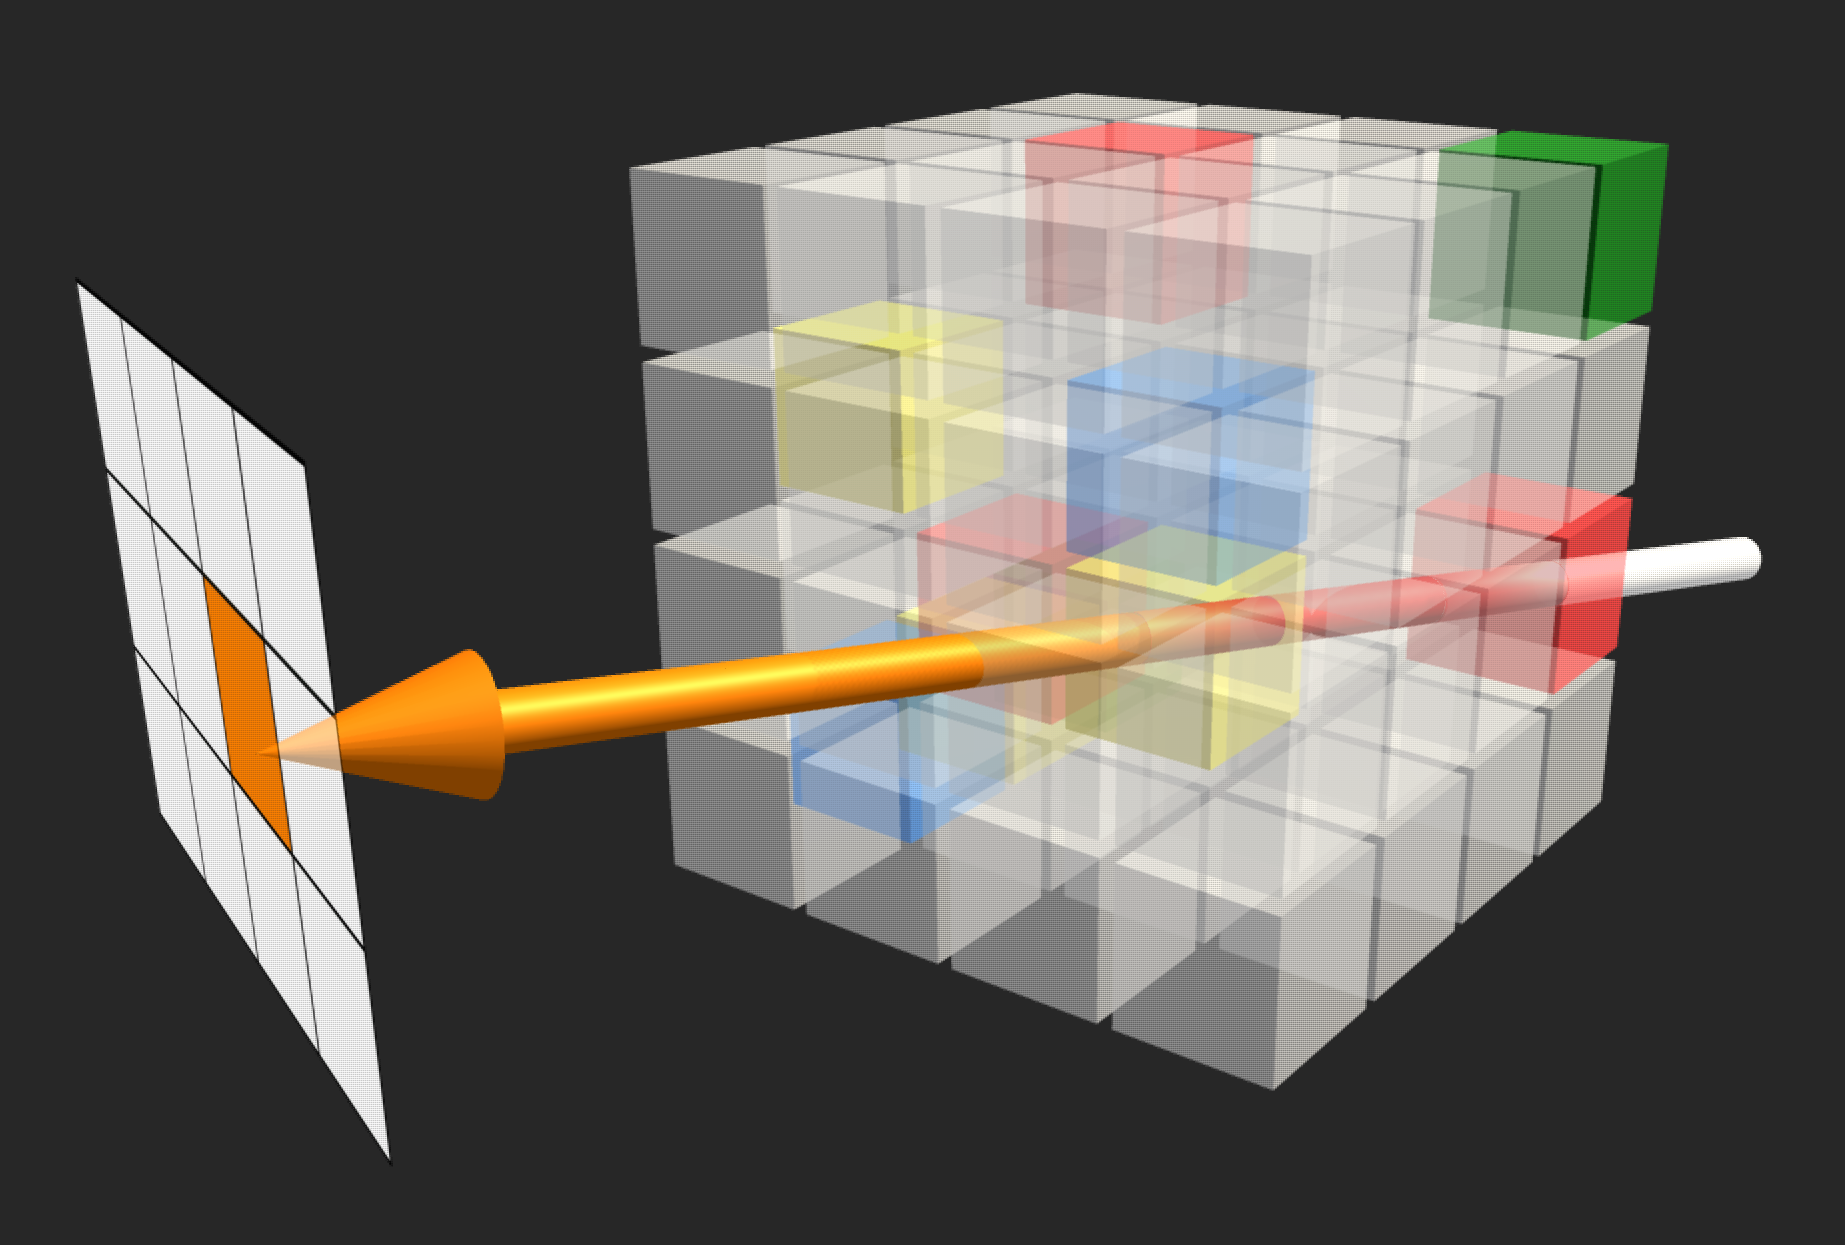
\includegraphics[width=1.0\textwidth]{ray-march-diagram}
\caption[FPBioimage: Raymarching facilitates volumetric rendering of 3D data]{In a traditional ray marching volumetric renderer, a colourless ray starts at the back of the volume, and picks up colour and transparency at each voxel it passes through. After its journey through the volume, it paints its accumulated colour to the screen pixel it lands on. }
\label{fig:raymarchDiagram}
\end{figure}

Volumetric rendering allows detail within the volume to be visualised. 
By tuning the opacity of each voxel, details which would be invisible in a surface rendering can be seen in context, through the outer voxels of the model. 

The key drawback of volumetric rendering compared to geometric rendering is speed. 
In the simple volumetric renderer shown in Figure~\ref{fig:raymarchDiagram}, a ray is calculated for each pixel on the screen - \num{2073600} pixels for a 1080p high definition display. 
If each ray takes \num{512} samples as it passes through the volume, each rendering of the volume requires \num{1061683200}. 

When rendering a single volumetric image, or even a video which is first rendered then presented at a later time, this is not an issue: the rays can computed in parallel across a cluster of computers, and with some patience the images will build up. 
However, until recently displaying volumetric data at video rate in real time required specialised hardware optimised solely for volumetric rendering. [cite patent??]

The gaming industry has led to a rapid development of devices optimised for performing thousands of simple calculations in parallel. 
A single graphics processing unit (GPU) contains as many as ??? individual processing cores, which can be used to calculate volumetric rays simultaneously. 
Combined with intelligent optimisations to the rendering algorithm, GPUs found in devices ranging from laboratory workstations to smartphones now enable real-time volumetric visualisation on personal computers. 

\subsection{WebGL}
Since the development of highly parallel GPUs, a handful of free and commercial software has been released which provide volumetric rendering capabilities. 
Popular programs used in the microscope community include ImageJ, Icy, and Imaris; [something and something] are also used in the medical community for visualising patient data. 
These programs provide advanced offline volumetric rendering, and FPBioimage is not designed to replace them; instead, the key feature of FPBioimage is providing rendering on the web, to facilitate easy and interactive sharing of 3D data. 

Creating this tool has only been possible because of the relatively recent invention and widespread adoption of the `Web Graphics Library' (WebGL), which provides access to a GPU's processing power directly from the web browser. 
This means that three-dimensional effects on webpages can be rendered to the screen in real time.

In technical terms, WebGL exposes the \texttt{OpenGL ES 2.0} feature set \cite{Khronos:WebGL}.
This is a shader-based application programming interface (API).
The API provides a limited number of simple functions which are optimised for running on GPUs in parallel. 

The support of WebGL is widespread, [cite canIuse, Figure~\ref{fig:caniusethis}, available through HTML5.

\begin{figure}[htb!]
\centering
\begin{subfigure}[b]{1.0\textwidth}
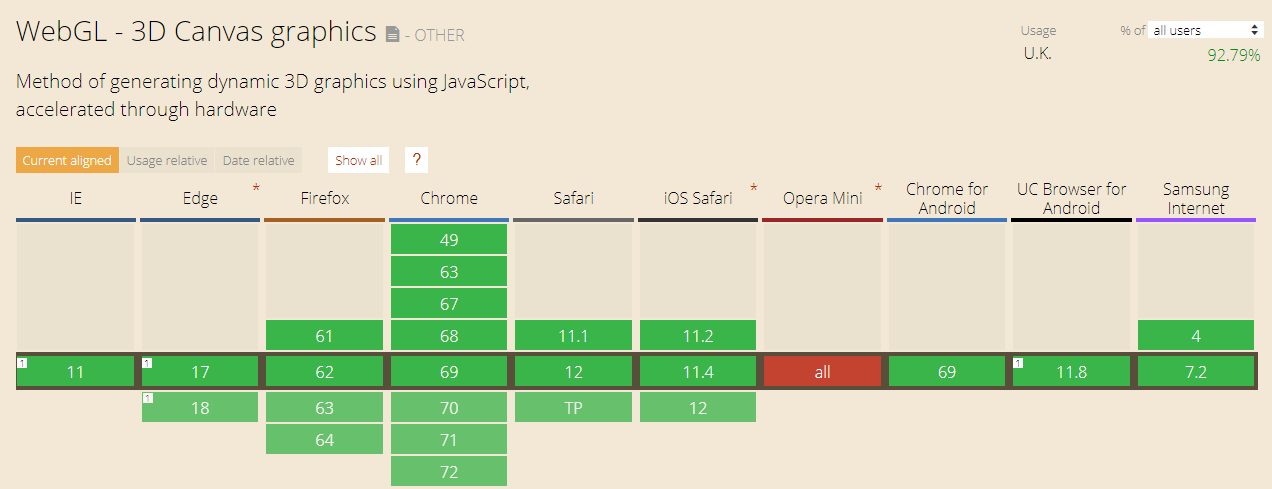
\includegraphics[width=1.0\textwidth]{caniusethis-webgl}
\caption{} \label{fig:caniusethis-webgl}
\end{subfigure}

~\newline
\begin{subfigure}[b]{1.0\textwidth}
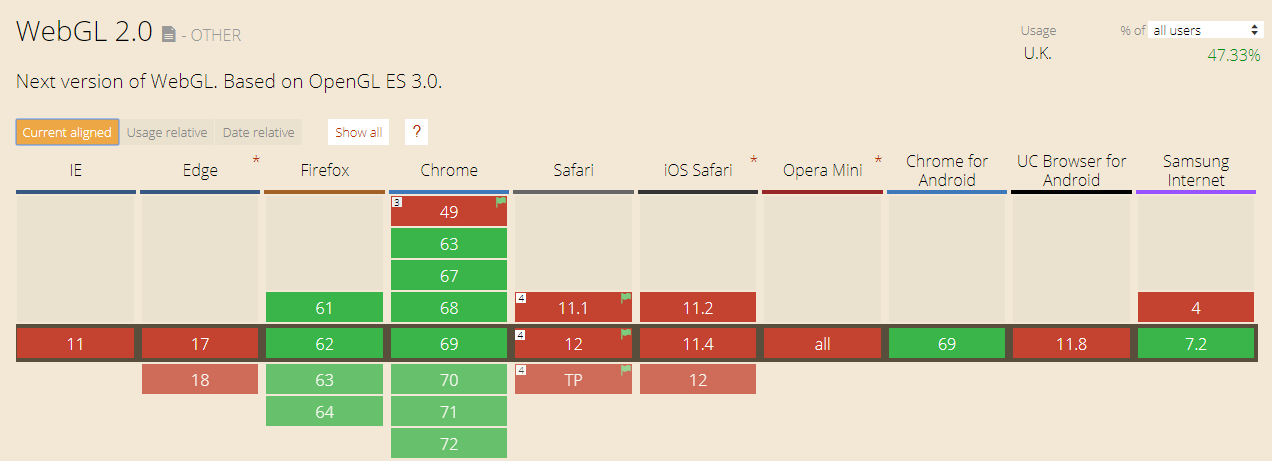
\includegraphics[width=1.0\textwidth]{caniusethis-webgl2}
\caption{} \label{fig:caniusethis-webgl2}
\end{subfigure}
\caption[FPBioimage: WebGL is supported by 92.79\% of users browsing the web]{Screenshots taken from \url{https://caniuse.com}\cite{caniuse}. (a) shows that FPBioimage, which is percentage built with WebGL, is supported by the web browsers of 92.79\% of UK users. Although WebGL 2.0 makes 3D programming easier, (b) shows that support would drop to 47.33\% of users.  }
\label{fig:caniusethis}
\end{figure}

A more modern version, WebGL 2.0, exposes the \texttt{OpenGL ES 3.0} API, which makes programming for 3D much easier.
However, at the time FPBioimage was published, support for WebGL 2.0 was highly limited. 
Even at the time of writing, WebGL 2.0 is only supported by third party browsers, and cannot be used in Microsoft's Edge or Apple's Safari, limiting it to just \SI{47.33}{\percent} of UK web users.

To maintain maximum compatibility, volumetric rendering in FPBioimage is implemented entirely in WebGL 1.0.
Various strategies for overcoming this restriction are detailed in Section~\ref{sec:shader}.

\subsection{Aims for FPBioimage} 
The primary goal for FPBioimage was to create an easy-to-use web application for visualising volumetric data in a web browser. 
The tool was required to run without requiring any other plugins or downloads, in order that viewing data was a simple process. 

After gathering user feedback, a list of desired features was compiled. 

\begin{enumerate}
	\item Rendering options for more advanced users
	\item Ability to cut the data open at arbitrary angles and positions (sometimes known as \textit{reslicing})
	\item Offter high resolution screenshots of the data
	\item Ability to save a particular view as a bookmark, and share that exact view with others
\end{enumerate}

For researchers sharing their own generated 3D data, more easy-to-use tools were proposed. 
These had to be compatible with popular image analysis programs, and facilitate fast sharing of volumetric data. 

From the first prototype FPBioimage was designed to be user-friendly. 
The program had to be intuitive so that a user could visualise their data without any training. 

\section{Method: software design} \label{sec:fpbSoftwareDesign}
This section describes, through the use of diagrams and code snippets, the method by which the volumetric visualisation software was developed.

The primary requirement of FPBioimage was that it must run in a web browser.
As mentioned in Section~\ref{sec:introvisual}, offline visualisation tools are already available, so the distinguishable feature of this software was the ability to share and publish volumetric data online.
For fast development and compatibility with multiple devices, I chose to develop the software in a game engine called Unity [cite].
This gives access to an extensive library of functions for creating dynamic 3D scenes, as well as a language for executing code on the graphics card.
When the software is complete, Unity allows the designer to compile the `game' into compressed HTML/Javascript code to run in a web browser.

\subsection{Fragment shader} \label{sec:shader}

\begin{lstlisting}[language=C,caption={Fragment shader code for volumetric ray marching},label={snip:renderloop},frame=single]
// Fragment shader
float4 frag(frag_input i) : COLOR
{
	// Calculate eye ray (i) intersection with cube bounding box
	float3 boxMin = { -0.5, -0.5, -0.5 };
	float3 boxMax = {  0.5,  0.5,  0.5 };
	float tNear, tFar;
	bool hit = IntersectBox(i.ray_o, i.ray_d, boxMin, boxMax, tNear, tFar);
	if (!hit) discard;
	if (tNear < 0.0) tNear = 0.0;

	// Calculate intersection points
	float3 pNear = i.ray_o + i.ray_d*tNear;
	float3 pFar  = i.ray_o + i.ray_d*tFar;
	// convert to texture space
	pNear = pNear + 0.5;
	pFar  = pFar  + 0.5;

	// March along ray inside the cube, accumulating color
	float3 ray_pos = pNear;
	float3 ray_dir = pFar - pNear;
	float3 ray_step = normalize(ray_dir) / _Steps;

	float normalised_opacity = _Opacity * length(ray_step);
	float4 ray_col = 0;
	float mean_max_voxel = 0;

	for(int k = 0; k < MAX_STEPS; k++){
		if (k<_Steps){
			// Get current position
			ray_pos = pNear + k * ray_step;

			// Clip if behind clip plane or outside unit cube
			bool clipVoxel = dot(_ClipPlane, float4(ray_pos-0.5f, 1.0f)) > 0.0f
			 || !(ray_pos.x > 0.0f && ray_pos.y > 0.0f && ray_pos.z > 0.0f
			  && ray_pos.x < 1.0f && ray_pos.y < 1.0f && ray_pos.z < 1.0f);

			if (!clipVoxel && ray_col.a < 1.0f){
			  	// Get colour of the voxel we're passing through
		  		float4 voxel_col = sample2D(ray_pos);
			  	float mean_col = (voxel_col.r + voxel_col.g + voxel_col.b);

			  	if (_RenderMode == 0 && mean_col > _Threshold){
			  		// Max Intensity Projection
		  			if (mean_col > mean_max_voxel){
		  				ray_col = voxel_col;
		  				mean_max_voxel = (voxel_col.r + voxel_col.g + voxel_col.b);
		  			}

			  	} else if (_RenderMode == 1 && mean_col > _Threshold){
					// Volumetric ray marching with transparency
					voxel_col.a *= normalised_opacity;
					voxel_col.rgb *= voxel_col.a;
					ray_col += (1.0f-ray_col.a) * voxel_col;

				}
			}
		}
	}
	ray_col.rgb *= _Intensity;
    return ray_col;
}
\end{lstlisting}

FPBioimage uses a ray marching technique similar to that presented in Section~\ref{sec:volumerendering}.
The main ray marching loop implementing this is shown in lines Snippet~\ref{snip:renderloop}.
This loop is part of the `fragment shader', which means it runs for every pixel rendered on the display.
It is therefore the most important loop in the whole program for efficiency, and any efforts to increase the speed at which this loop executes will be amplified by the number of pixels.
We will now examine the loop, and the efficiency modifications which have been made compared to traditional ray marching.

We should first start at lines 40 and 47, and note that there are two render modes: a maximum intensity projection (\texttt{\char`_RenderMode 0}) and the volumetric ray marching mode (\texttt{\char`_RenderMode 1}) discussed in section \ref{sec:volumerendering}.
In the maximum intensity projection mode, the ray checks the mean colour of every voxel it passes through, and paints the colour of the voxel with the largest `mean color' to the screen pixel.
Note that mean colour is calculated as the sum of the red, green, and blue colour channels.
Strictly we should divide by $3$ to calculate the true mean colour value; however, this would mean 2 extra divisions for every loop iteration for every pixel on the screen; removing this step has no effect on the comparison, but gives a noticeable improvement in frames rendered per second. % Do I want to put a graph of this?

Before discussing the volumetric ray marching calculation, we should note that in this implementation the ray marches from the screen to the back of the cube - this is the opposite of traditional scheme shown in Figure~\ref{fig:raymarchdiagram}.
The reason for this is, of course, efficiency.
As a ray progresses from a pixel through the cube, it becomes more and more opaque, denoted by the alpha value of the colour \texttt{ray\char`_col.a}.
Once the alpha value reaches 1, any voxels further along the ray's path will not be visible, so there is no reason to look up their colour or add their contribution to the ray.
Line 38's second condition is that \texttt{ray\char`_col.a < 1.0f} to implement this action.
Note that in most programming languages we would break out of the loop at this point, but WebGL 1.0 loops must have a constant number of iterations.

The requirement to have a constant number of iterations also explains the very first condition in the loop on line 29.
The variable \texttt{k\char`_Steps} sets the depth resolution of the volume.
We might expect the \texttt{for} loop to finish when \texttt{k < k\char`_Steps}, but this would set the depth resolution as a constant, so that there was no option to increase it for powerful machines or decrease it for mobile devices.
By looping for \texttt{MAX\char`_STEPS} iterations (which is currently set to 512, but could be increased as hardware improves in the future) but performing no calculations if the loop variables \texttt{k} is greater than \texttt{k\char`_STEPS}, we can still set the depth resolution to integer from 0 to \texttt{MAX\char`_STEPS} and gain a performance benefit for low resolutions.

There are two additional conditions which must be met for the volume renderer to add a voxel to the ray.
Firstly, shown in line 38, the ray position must be within the unit cube and behind the clip plane.
The clip plane can be used to cut open the volumetric model at any angle and position, and is described in more detail in Section~\ref{sec:fpbresults}.
Secondly, the voxel's mean colour intensity must fall about the value of \texttt{\char`_Threshold} to contribute to the ray, ensuring that dark voxels around the volume are not visible.

If all the aforementioned conditions are met, then the code in lines 49 - 51 performs the volumetric ray marching step - that is, the colour of the current voxel mixes onto the ray that is passing through it.
Firstly, the voxel's opacity is adjusted based on the input variable \texttt{\char`_Opacity}, which allows the volume to be rendered with transparency.
This new value of alpha is multiplied onto the voxel's colour so that more transparent voxels contribute less intensity to the ray.
Finally, the adjusted voxel is added to the ray, with its contribution weighted by the current transparency of the ray.

\subsection{Loading 3D data in WebGL} \label{sec:fpbVolumeRendering}
To render volumetric images using the graphics card, the volumetric data must be loaded onto the graphics card in an appropriate form.
WebGL 2.0 provides a \texttt{sample3D} class, which is able to store 3D images and return a voxel colour at a requested 3D coordinate.
Unfortunately WebGL 1.0 does not have this functionality, and so an alternative scheme based on 2D textures has been devised.

The simplest way to picture volumetric imaging data is as a z-stack of 2D image slices.
One option to obtain a voxel colour at a given $xyz$-coordinate would be to store all 2D image slices, and look up the $xy$ value of the appropriate slice based on the $z$-coordinate.
This is conceptually simple, but inefficient to implement on a graphics card, as each slice must be sent to the graphics card individually, which is not only slow but adds a significant memory overhead to the graphics card loading process. [cite texture atlases?]
Instead, I devised a scheme where slices are stored on a large 2D texture atlas in a grid pattern.
Then, a $z$-coordinate corresponds to a specific slice on the grid, and the $xy$ components can be added to the bottom-left coordinates of that slice to get the $xyz$-coordinate voxel colour.

A restriction of WebGL 1.0 is a maximum texutre size of 4096$\times$4096.
Using the atlas technique, this would support a maximum voxel resolution of 256$\times$256$\times$256.
This was found to be inadequate for most researcher's data, so a target of 512$\times$512$\times$512 was set.
In order to meet the requirements of WebGL 1.0, this requires 8 2D texture atlases of size 4096$\times$4096.

The 8 texture atlases are filled according to the pseudo-code shown in Snippet~\ref{snip:textureloading}.
The code uses a mixture of the modulo operator (\%) and division (\/) to determine (a) which atlas to place each volume image slice in, and (b) the location in that image where the slice should be located.
Complementary code runs in the WebGL rendering code to read a particular voxel's colour given an $xyz$-coordinate.

\begin{lstlisting}[language=java,caption={Pseudo-java code for 3D texture atlas arrangement},label={snip:textureloading}]
int sliceWidth = volumeImage.width;
int sliceHeight = volumeImage.height;
int numSlices = volumeImage.depth; // Number of z-slices

int atlasWidth; int atlasHeight;
int numberOfAtlases = 8;

// Pad image size up to next power of 2
int paddedSliceWidth = ceil2(sliceWidth);
int paddedSliceHeight = ceil2(sliceHeight);

int xOffset = (int)Math.floor((paddedSliceWidth - sliceWidth)/2);
int yOffset = (int)Math.floor((paddedSliceHeight - sliceHeight)/2);

// Calculate the xy size of the atlases, making atlases as square as possible
int slicesPerAtlas = (int)Math.ceil((float)numSlices/(float)numberOfAtlases);
atlasWidth = ceil2(paddedSliceWidth);
atlasHeight = ceil2(paddedSliceHeight * slicesPerAtlas);
while((atlasHeight > 2*atlasWidth) && (atlasHeight > sliceHeight)) {
	atlasHeight /= 2;
	atlasWidth *= 2;
}

// Initialise an array of 8 black 2D textures to become atlases
Image[] atlasArray = new Image[numberOfAtlases];
for (int i=0; i<numberOfAtlases; i++){
	atlasArray[i] = new Image(atlasWidth, atlasHeight, black);
}

// Fill out atlases with image slices
int slicesPerRow = (int)Math.floor((float)atlasWidth/(float)paddedSliceWidth);
for (int i=0; i<numSlices; i++){
	int atlasNumber = (int)((float)i % (float)numberOfAtlases);
	int locationIndex = (int)Math.floor((float)i/(float)numberOfAtlases);

	// Get slice
	Image slice = volumeImage.getSlice(i);

	// Put slice into atlas at the correct position
	int xStartPixel = (int)((float)locationIndex % (float)slicesPerRow) * paddedSliceWidth + xOffset;
	int yStartPixel = (int)Math.floor((float)locationIndex / (float)slicesPerRow) * paddedSliceHeight + yOffset;

	// The following line should be uncommented for coordinate systems that start top-left
	//yStartPixel = atlasHeight - yStartPixel - paddedSliceHeight + 2*yOffset;

	copySubImageToAtlas(sliceTexture, atlasArray[atlasNumber], xStartPixel, yStartPixel);
}
\end{lstlisting}

% Should I add some paragraphs here about XY and Z resolution? Probably should.
%subsection{Rendering optimisation}
% XY resolution can be adjusted cleverly. 

% Z resolution can also be adjusted

% Interpolation

% Rendering paused when there is no user input. 

\subsection{Movement and control}
It would not make for a particularly exciting real-time volumetric renderer if the user only had one view of the data.
Thanks to the Unity library functions, implementing movement is a straightforward and resource-efficient process.

Firstly, as with all offline volumetric rendering programs, the 3D model can be rotate about its $x$-, $y$- and $z$-axes to view a different part of the data.
This is achieved in Unity by mapping the volume rendering shader described in Section~\ref{sec:shader} onto a cube.
The cube is then linked to both the arrow keys and the mouse to provide intuitive manipulation of the volume, as shown in Snippet~\ref{snip:cuberotation}.
For data whose combination of $xyz$ resolution and $xyz$ voxel size describes a cuboid, the $xyz$ scale of the rendering cube can be adjusted to ensure distortion-free visualisation.

\begin{lstlisting}[language={[Sharp]c}, label={snip:cuberotation}, caption={C\# code using built-in Unity functions to rotate the rendered volumetric data.}]
void FixedUpdate () {
	// This code is attached to the rendering cube, and called once per frame

	// Keyboard arrow control
	Vector3 vertRotAxis = transform.InverseTransformDirection(camera.TransformDirection(Vector3.right)).normalized;

	float horizontalRot = Input.GetAxis("H2");
	float verticalRot = Input.GetAxis("V2");

	transform.Rotate(vertRotAxis, verticalRot, Space.Self);
	transform.Rotate (Vector3.up, horizontalRot, Space.World);

	// Mouse click control
	if(Input.GetMouseButton(0)){
		// Rotate with the mouse
		Vector3 vertRotAxis = transform.InverseTransformDirection(camera.TransformDirection(Vector3.right)).normalized;

		float horizontalRot = Input.GetAxis("Mouse X");
		float verticalRot = Input.GetAxis("Mouse Y");

		transform.Rotate(vertRotAxis, verticalRot, Space.Self);
		transform.Rotate (Vector3.up, horizontalRot, Space.World);
	}
}
\end{lstlisting}

The `FP' in FPBioimage actually stands for `First Person,' and refers to the control the user has over the scene's camera.
Rather than just viewing the rotatable render cube from one perspective, as in common in offline volumetric renderers, FPBioimage allows the user to change the position and look-direction of the camera.
This is implemented as shown in Snippet~\ref{sec:cameramovement}.
The \texttt{H1} axis is mapped to the A and D keys, and the \texttt{Z1} axis to the W and S keys.
This, combined with the functionality of using the mouse to change the camera's look-direction, will make control of the camera very familiar to anyone who has played first person perspective computer games.
Moving the camera allows the user to create the type of dynamic fly-bys sometimes seen in publication videos in real time, providing a highly immersive visualisation of the data.

\begin{lstlisting}[language={[Sharp]c}, label={sec:cameramovement}, caption={C\# code using built-in Unity functions for moving the camera in a first-person manner.}]
void FixedUpdate(){
	// Translation
	transform.position += Input.GetAxis ("V1") * Camera.main.transform.up * Time.deltaTime;
	transform.position += Input.GetAxis ("H1") * Camera.main.transform.right * Time.deltaTime;
	transform.position += Input.GetAxis ("Z1") * Camera.main.transform.forward * Time.deltaTime;
	transform.position += Input.GetAxis ("Mouse ScrollWheel") * Camera.main.transform.forward * Time.deltaTime;

	// Rotation
	if (!Input.GetMouseButton(1)) {
		// This is the 'first person' mouse mode
		rotationX += (Input.GetAxis ("Mouse X")) * mouseSpeed;
		rotationY += (Input.GetAxis ("Mouse Y")) * mouseSpeed;
		rotationY = ClampAngle (rotationY, minimumY, maximumY); // Stops camera doing backflips!

		Quaternion xQuaternion = Quaternion.AngleAxis (rotationX, Vector3.up);
		Quaternion yQuaternion = Quaternion.AngleAxis (rotationY, -Vector3.right);

		transform.localRotation = startRotation * xQuaternion * yQuaternion;
	}

	// Camera movement with mouse
	if (Input.GetMouseButton (1)) {
		transform.position -= Input.GetAxis("Mouse X") * Camera.main.transform.right * Time.deltaTime / Screen.width;
		transform.position -= Input.GetAxis("Mouse Y") * Camera.main.transform.up * Time.deltaTime / Screen.height;
	}
}
\end{lstlisting}

\subsection{Bookmarking}
FPBioimage implements a bookmarking function to save a particular view with an annotation.
The bookmarked view can then be shared with others as a web link, or restored on the same computer at a later time.

To implement the bookmark saving and restoring into the user interface requires several distinct stages depending on the user's input.
An elegant method for reliably moving the user between these stages is a state machine.
The state machine controlling the bookmark saving and restoration procedures is shown in Figure~\ref{fig:bookmarking-state-machine}, and can be described as follows:
\begin{tabular}{>{\bfseries}l p{0.85\textwidth}}
State 0 & The default state, where all states eventually return to. Nothing regarding bookmarking is shown on the screen. Pressing `B' on the keyboard will start the bookmark creation process; pressing a number key will start the bookmark restoration process. Any other key does not change the state. \\
State 1 & The bookmarking textbox pops up requesting the user to enter a number key to save the new bookmark in that position. Pressing a number key will take the user to the next stage of bookmark creation; pressing `Escape' will close the textbox and return to the default state. \\
State 2 & The user can enter a text annotation into the text box. Pressing `Escape' will immediately close the textbox and return to the default state; pressing `Return' (also known as `Enter') will save the bookmark as described below and move to State 3. Note that an empty annotation is accepted. \\
State 3 & This state displays information or annotation text. If arriving from State 2, it will show a confirmation message; if arriving from State 4, it will show the annotation text saved alongside the bookmark being restored. \\
State 4 & This state simply checks that the volumetric model has loaded, to ensure no error is thrown if trying to restore a bookmark on an uninitialised volume. The state machine continues to wait in State 4 if the volume is loading, so any requested bookmark will be loaded immediately when the volume is ready. \\
\end{tabular}

\begin{figure}[htbp!]
\centering
\includegraphics[width=1.0\textwidth]{bookmarking-state-machine}
\caption[FPBioimage: Bookmark creation and restoration is controlled by a state machine]{The state machine shown controls the creation and restoration of bookmarks. }
\label{fig:bookmarking-state-machine}
\end{figure}

Internally, the bookmarks are encoded as JavaScript Object Notation (JSON) strings, converted to a base-64 string, and then saved to the web browser's `Local Storage'.
Saving to Local Storage requires the C\# program to interface with the web browser through Javascript.
Unity provides the function \texttt{ExternalEval(string jscode)} to complete this task, where \texttt{jscode} is a string containing the JavaScript code to be executed.
Once the bookmark has been encoded, it is saved to the web browser as shown in lines 1 and 2 of Snippet~\ref{snip:savingbookmark}.
The bookmark is saved to Local Storage with a unique prefix followed by the bookmark's number, so that it can be restored at a later time.

\begin{lstlisting}[language={[Sharp]c}, label={snip:savingbookmark}, caption={C\#-JavaScript interface code for interacting with the browser's local storage to save and share bookmarks.}]
string evalMe = "localStorage.setItem('fpb-" + variables.fpbJSON.uniqueName + "-bookmark" + bookmarkNumber + "', '" + bookmarkString64ToSave + "');";
Application.ExternalEval (evalMe);
evalMe = "history.replaceState(null, null, '?b=" + bookmarkString64ToSave + "');";
Application.ExternalEval (evalMe);
\end{lstlisting}

Lines 3 and 4 of Snippet~\ref{snip:savingbookmark} shows how the base-64 bookmark string is appended to the base url in the web browser using the JavaScript function \texttt{replaceState}.
The user can then simply copy the URL and send it to a friend or colleague to open on their own computer.
When the volume is being loaded, the bookmarking C\# script checks the URL of the webpage its running on, and if it finds a "\texttt{?b=}" in the URL string it will begin restoring the bookmark.
This puts the bookmarking state machine into State 4, ready to show the bookmark and annotation text as soon as the volumetric model has loaded.
In this way users can easily share specific views of the data across the globe.

\subsection{Capturing screenshots}
FPBioimage provides the capture of high resolution screenshots, shown in Snippet~\ref{snip:screenshots}.

When the \texttt{takeScreenshot} function is called, a new \texttt{RenderTexture} is created to save the current view to.
The size of this can be set either by the current pixel size of the main camera or by user input.
In this way screenshots at a higher resolution than the current view can be created.
This is advantageous, as the user can view the volumetric data in small window for fast performance, but then take a single screenshot at a high resolution for presentation and publication.

The new render texture is converted to a PNG-encoded byte stream, and then offered to the user as a download through the Javascript library \texttt{download.js}.
\texttt{download.js} provides a single function \texttt{download(data, strFileName, strMimeType)}, which is called from Unity using the C\#-Javascript interface function \texttt{ExternalCall}.
This is shown in line 32 of Snippet~\ref{snip:screenshots}.

\begin{lstlisting}[language={[Sharp]c}, label={snip:screenshots}, caption={C\# code for capturing a high-resolution screenshot and presenting it to the user as a download.}]
public void takeSreenshot(bool hiRes){
	if (hiRes) {
		bool wOK = int.TryParse (wRes.text, out ssWidth);
		bool hOK = int.TryParse (hRes.text, out ssHeight);

		if (!wOK || ssWidth < 1) {
			ssWidth = 1920;
		}
		if (!hOK || ssWidth < 1) {
			ssWidth = 1080;
		}
	} else {
		ssWidth = Camera.main.pixelWidth;
		ssWidth = Camera.main.pixelHeight;
	}

	// Create screenshot-sized render texture to render to
	RenderTexture rt = new RenderTexture(ssWidth, ssWidth, 24);
	mainCamera.targetTexture = rt;
	Texture2D snapShot = new Texture2D(ssWidth, ssWidth, TextureFormat.RGB24, false);
	mainCamera.Render();
	RenderTexture.active = rt;
	snapShot.ReadPixels(new Rect(0, 0, ssWidth, ssWidth), 0, 0);
	mainCamera.targetTexture = null;
	RenderTexture.active = null;
	Destroy(rt);

	// Encode snapshot to PNG byte stream
	byte[] bytes = snapShot.EncodeToPNG ();

	// Offer screenshot as download
	Application.ExternalCall ("download", "data:image/png;base64," + System.Convert.ToBase64String (bytes), "Screenshot " + System.DateTime.Now.ToString ("yyyy-MM-dd") + " at " + System.DateTime.Now.ToString ("HH.mm.ss") + ".png", "image/png");
}
\end{lstlisting}

\section{Results and discussion} \label{sec:fpbResults}
The FPBioimage software designed in Unity, as detailed in Section~\ref{sec:fpbSoftwareDesign}, was compiled into JavaScript to run in a web browser.
In this section, all screenshots and tests were performed in Google Chrome version 58 on the Windows 10 operating system.
However FPBioimage also runs without issue on any modern web browser, including Mozilla Firefox, Microsoft Edge, and Apple Safari, including mobile versions of these browsers.

\subsection{User interface}
Much care has been taken to ensure FPBioimage is a user-friendly piece of software.
Many offline software packages already exist for rendering volumetric data; FPBioimage's unique selling point is that it runs in a web browser, to make sharing data with colleagues across the world a simple process.
For this reason it is important that a non-expert user can simply browse to a website and use the software without any training.
At the same time, whilst being immediately accessible to new users the software contains a number of advanced rendering options for those wishing to extract more information from the data.

\begin{figure}[htbp!]
\centering
\includegraphics[width=1.0\textwidth]{fpb-start-screen}
\caption[FPBioimage: Users are presented with a simple interface which is intuitive to use]{When a user opens an FPBioimage webpage, the data will be downloaded and the user will be presented with the simple interface shown. The model can be interacted with intuitively by clicking and dragging with the mouse, or finger on a touchscreen. The data shows a C. Elegans embryo captured by single plane illumination microscopy (SPIM), provided by Hari Shroff~\cite{kumar2014dual}. }
\label{fig:FPBhome}
\end{figure}

When opening up a web link with FPBioimage on the page, the user is presented with the view shown in Figure~\ref{fig:FPBhome}.
Interacting with the volumetric model is responsive and intuitive.
Using the mouse, the user can rotate the volume by clicking and dragging, or on a touch screen by dragging with their finger.
Alternatively the arrow keys can be used on a keyboard.
Pinching on a touch screen, or using the scroll wheel on a mouse, zooms in and out of the model.
This creates a natural interaction with the data that requires no additional instruction.

\begin{figure}[htbp!]
\centering
\includegraphics[width=1.0\textwidth]{fpb-side-panels}
\caption[FPBioimage: Side panels provide more advanced rendering options]{Clicking on the side panel arrows slides in advanced rendering options, clipping plane options, quality options, and bookmark and sharing options. Data from~\cite{kumar2014dual}. } % 
\label{fig:FPBpanels}
\end{figure}

To access more advanced rendering features, Figure~\ref{fig:FPBpanels} a panel on the right-hand side of the screen which slides in.
The user is presented with 3 rendering parameters: \textui{Opacity}, \textui{Intensity}, and \textui{Threshold}.
Matching these parameters up to the volume rendering code described in Section~\ref{sec:fpbVolumeRendering}, it is easy to see how each parameter modifies the presentation of the data.

\begin{figure}[htbp!]
\centering
\includegraphics[width=1.0\textwidth]{fpb-sliders-examples}
\caption[FPBioimage: Advanced rendering features provide unique views of volumetric data]{(a–c): Four-colour OPT data of a mouse embryo. (d–f): MRI data of a human head. (g–i): two-colour light-sheet microscopy data of a drosophila embryo. FPBioimage's built-in transparency feature has been used to render (c) and (f), revealing data within the volume; the cutting tool has been used for (c), (f), (h) and (i), removing outer voxels from the data; and h shows a bookmark in creation, which can be shared with other users. Reproduced from \cite{fantham2017new}. Raw data provided by: (a–c), J. McGinty~\cite{sharpe2002optical}; (d–f), Stanford Volume Data Archive~\cite{levoy1988volume}; (g–i), P. Keller~\cite{chhetri2015whole}. }
\label{fig:fpbRendering}
\end{figure}

Lowering the \textui{Opacity} value means that each voxel contributes less alpha to the ray marching through it; consequently, the volumetric data becomes more transparent.
This makes features inside the model visible through the outer voxels, as shown in Figure~\ref{fig:fpbRendering}.
Combined with rotating the volume, this facilitates visualisation of how different structures are arranged in 3D space, providing answers that are not possible to obtain in any other way.

The \textui{Intensity} value acts globally on the data at the end of the ray marching process.
This simply increases or decreases the overall brightness of the model, to reveal contrast either at the bright end or the dark end of voxel values. % should I actually make this change the response curve??

The \textui{Threshold} slider sets the value below which voxels are not rendered.
Most microscopy images, as well as images from other modalities such as MRI, use black voxels around the imaging data to represent a lack of light or objects.
Settings a small positive value for \textui{Threshold} ensures that the volume does not appear as a black box when \textui{Opacity} is set high.
Larger values for \textui{Threshold} can also be used to highlight bright objects which lie within the volume.

The next element in the right-hand UI tab is the \textui{Projection} dropdown menu.
As described in Section~\ref{sec:fpbSoftwareDesign}, FPBioimage provides several volumetric visualisation rendering pipelines.
These include \textui{Max. Intensity}, which renders a maximum intensity projection from any angle; \textui{Composite}, which performs volumetric ray tracing with support for transparency; and \textui{Iso-surface}, which reveals only voxels within a certain percentage of the \textui{Threshold} cutoff.
Screenshots of the various \textui{Projection} methods rendering a [something!!] are shown in Figure~\ref{fig:fpbProjections}.

\begin{figure}[htbp!]
\centering
\includegraphics[width=1.0\textwidth]{fpb-projections}
\caption[FPBioimage: Four projection methods highlight different details in volumetric data]{First Person Bioimage offers 4 different types of volumetric projection. (a) shows a maximum intensity projection, (b) a volumetric ray marching projection, (c) a variation on the volumetric ray marching projection, with alpha calculated from RGB voxel values, and (d) an iso-surface projection. Data is of a mouse embryo head captured with `OPTiSPIM', provided by Jim Swoger~\cite{mayer2014optispim}. }
\label{fig:fpbProjections}
\end{figure}

Further down the right-hand UI tab are two UI buttons for capturing screenshots.
The first, \textui{Take shot}, captures a screenshot at the current resolution of the drawing canvas.
Perhaps more usefully, the \textui{High resolution} screenshot button captures a screenshot at the resolution defined in the two text boxes below.
This allows the user to capture screenshots at a higher resolution than their display, in case high resolution images are required for presentation or publication.
The advantage of this is exemplified in Figure~\ref{fig:fpbScreenshots}.

\begin{figure}[htbp!]
\centering
\begin{subfigure}[b]{1.0\textwidth}
\includegraphics[width=1.0\textwidth]{fpb-screenshot-low}
\caption{}
\end{subfigure}

~\newline
\begin{subfigure}[b]{1.0\textwidth}
\includegraphics[width=1.0\textwidth]{fpb-screenshot-high}
\caption{}
\end{subfigure}
\caption[FPBioimage: Screenshots allow views to be captured at a higher resolution than the user's display]{High resolution screenshots can be created even on a small display. (a) shows a screenshot at the native 768x1024 display resolution; (b) shows a 1080p screenshot of the same view, created using the \textui{High resolution} button. Images are of mitochondria captured with a whole-cell 4Pi single-molecule switching nanoscopy (W-4PiSMSN) microscope, provided by Joerg Bewersdorf~\cite{huang2016ultra}. }
\label{fig:fpbScreenshots}
\end{figure}

The final two buttons in the right-hand UI tab are toggle buttons, labelled \textui{FP mode} and \textui{Keyboard}.
\textui{FP mode} toggles on the First Person mouse control that gives FPBioimage its full name.
In this mode the user can use the mouse to look around, in a way that is familiar to anyone who has played a first-person perspective game.
This can provide dramatic and immersive flights through the data controlled by the user, revealing much more information than can be provided on a pre-recorded video.
First Person control is shown in Video [??] in the online version of this thesis, or in Supplementary Video [??] provided on the CD/USB drive.

At all times (except when creating a bookmark), the user can use the WASD keys to move around, as shown when the \textui{Keyboard} button is active.
Pressing the \textui{Keyboard} button brings up a full list of controls, presented in Figure~\ref{fig:fpbMenu}.
Every rendering option is available through a keyboard shortcut, for complete mouse-free operation.

\begin{figure}[tbp!]
\centering
\includegraphics[width=1.0\textwidth]{fpb-menu}
\caption[FPBioimage: Keyboard controls allow FPBioimage to be used without a mouse]{All rendering options in FPBioimage can be controlled by the keyboard, for mouse-free operation. The teapot in the background is the widely available Utah teapot created by Martin Newell~\cite{torrence2006martin}. }
\label{fig:fpbMenu}
\end{figure}

The left-hand UI tab reveals yet more parameters which can be controlled by a more advanced user.

The first of these is \textui{Quality}.
Volume rendering in real time is a graphics intensive operation which has only recently become possible, and there is a clear trade off between quality and performance on most computers or mobile devices.
A dropdown list with a number of preset options with suggestions of the type of device they are suitable for.
For more advanced users, the individual quality settings \textui{XY Resolution}, \textui{Z Resolution}, and \textui{Interpolation} can be adjusted independently.
The \textui{Quality} settings are saved to the web browser's Local Storage upon modification and are automatically restored on the user's next visit to an FPBioimage webpage.
The performance-quality trade-off is discussed in more detail in Section~\ref{sec:fpbPerformance}.

The bookmarking functionality can be accessed from the UI using the \textui{Save} and \textui{Restore} buttons.
This begins the process shown in Figure~\ref{fig:bookmarking-state-machine}.
Creation of a bookmark is shown in Figure~\ref{fig:fpbBookmarkCreation}.
When a bookmark is created or restored, the URL in the browser bar changes to encode the bookmark as a web link.
This link can then be shared with other users, by email, text, or on social media, who will see exactly the same view when FPBioimage loads.
This is demonstrated in Figure~\ref{fig:fpbBookmarkRestoration}, where the shared bookmark is opened on another computer, with a different browser and operating system.

\begin{figure}[htbp!]
\centering
\centering
\begin{subfigure}[b]{1.0\textwidth}
\includegraphics[width=1.0\textwidth]{fpb-bookmarks}
\caption{} \label{fig:fpbBookmarkCreation}
\end{subfigure}

~\newline
\begin{subfigure}[b]{1.0\textwidth}
\includegraphics[width=1.0\textwidth]{fpb-bookmark-sharing}
\caption{} \label{fig:fpbBookmarkRecieved}
\end{subfigure}
\caption[FPBioimage: Bookmarks can be shared as a URL for another user to open]{(a) shows creation of a bookmark, with an annotation, in the Firefox web browser running on Windows 10. The bookmark can be restored on the same computer, or shared as a URL to another user. (b) shows the same bookmarked view in Apple Safari running on macOS 10.13 High Sierra. The MRI scan of a lemon was provided by Joe Cooper. }
\label{fig:fpbBookmarks}
\end{figure}

Finally, at the bottom of the left-hand UI tab are the UI buttons for the clipping plane.
Mentioned briefly in Section~\ref{sec:fpbVolumeRendering}, the clipping plane prevents voxels that are behind it from being rendered, revealing voxels inside the volumetric data that are otherwise obscured.
The clipping plane's location is controlled with the IJKL keys, where I and K are used to move the clipping plane forward and back, and J and L rotate is around to cut the data at an arbitrary angle.
Once an interesting cut has been made, the clipping plane can be locked in place with respect to the model by pressing the \textui{Lock Plane} button.
With the clipping plane locked, the user can move the camera or the model to view the cut volumetric data from a different angle.
Use of the clipping plane can therefore provide insightful perspectives of the volumetric data that are not possible to obtain with any other method, as shown in Figure~\ref{fig:fpbClippingPlane}.

\subsection{Performance} \label{sec:fpbPerformance}
Until recently, volume rendering was not possible in real time, and would be calculated given a specific camera perspective in advance to render either a single image or video.
In [some year], [some company] produced the [some device name], a dedicated piece of hardware which could render [512$\times$512$\times$512] volumetric images in real time.
This was achieved by realising the volume rendering algorithm described in Section~\ref{sec:volumerendering} with physical devices, with [??] calculations running in parallel to compute all rays at once. [cite]
Today, top-end graphics cards are able to perform the same calculations in real time on a Graphics Processing Unit (GPU), a highly parallelised device optimised for computing lighting models. [cite]

A primary aim of FPBioimage was that it should be user-friendly, with a particular focus on ease of use for non-expert users viewing data.
It was therefore expected that a majority of users would not have access to expensive, high-performance graphics cards required for rendering volumetric data in real time at full resolution.
Furthermore FPBioimage was designed so that it could be run on any device - according to [somewhere], [some percentage\%] of users to the [Nature?] website accessed articles through a mobile browser.
In order to support the full range of users, it was important to devise a scheme where the user could reduce the quality of the volume rendering in exchange for an increase in performance.

In the computer games industry, ``performance'' essentially means how many frames are rendered to the screen per second - assuming the graphics card is working at full capacity.
If the graphics rendering does not require the full capacity of the graphics card, performance can be measured as the percentage of the graphics card's compute capabilities in use.
In the tests presented in this chapter, performance is given in both frames per second (FPS) and graphics card usage percentage, measured using Windows Task Manager.
Screenshots of the software under test are shown in Figure~\ref{fig:fpbTestScreenshots}.

``Quality'' is harder to define.
For a scene of simple 2D geometry quality could be measured by the XY-resolution of the screen, and we would expect performance to decrease as XY-resolution increases.
For our volumetric data, however, we also have a Z-resolution, represented in Snippet~\ref{snip:renderloop} as \texttt{\char`_Steps}.
Furthermore visual quality is improved if, instead of just taking the nearest voxel to the tip of the marching ray, interpolation is performed between either the 2 or 8 closest voxels.

The three quality parameters can be adjusted as user inputs, or preset values can be selected.
A table of quality against performance for different combinations of the three quality metrics, and for the preset values, is shown in Table~\ref{tab:fpbPerformance}. 

\begin{table}
\caption[FPBioimage: quality and performance]{\label{tab:fpbPerformance}The table shows how performance, measured by FPS and GPU percentage use, is affected by the FPBioimage quality settings. This test was performed on a midrange laptop, which cost £580 in 2017, with the following specification: 2-core i5-7200U\,@\SI{2.50}{\giga\hertz}, \SI{8}{\giga\byte} RAM, NVIDIA GeForce GTX 1050 with \SI{4}{\giga\byte} graphics RAM.}
\begin{tabular}{|l l|c c c|c c|}
\hline
\multicolumn{2}{|c|}{Preset} & \multicolumn{3}{c|}{Quality} & \multicolumn{2}{c|}{Performance} \\
\multicolumn{1}{|c}{Name} & \multicolumn{1}{c|}{Device} & XY-res. & Z-res. & \multicolumn{1}{c|}{Interp.} & FPS & \multicolumn{1}{c|}{GPU use} \\
\hline

\multicolumn{7}{|c|}{\textbf{XY-resolution test}} \\ \hline
\multicolumn{2}{|c|}{-} & 256 & 256 & 1X & 60 & 14\% \\
\multicolumn{2}{|c|}{-} & 768 & 256 & 1X & 60 & 41\% \\
\multicolumn{2}{|c|}{-} & 1024 & 256 & 1X & 60 & 63\% \\
\multicolumn{2}{|c|}{-} & 2048 & 256 & 1X & 41 & 88\% \\
 & & & & & & \\
\hline

\multicolumn{7}{|c|}{\textbf{Z-resolution test}} \\ \hline
\multicolumn{2}{|c|}{-} & 450 & 64 & 1X & 60 & 15\% \\
\multicolumn{2}{|c|}{-} & 450 & 256 & 1X & 60 & 21\% \\
\multicolumn{2}{|c|}{-} & 450 & 512 & 1X & 60 & 30\% \\
\multicolumn{2}{|c|}{-} & 450 & 768 & 1X & 60 & 39\% \\
 & & & & & & \\
\hline

\multicolumn{7}{|c|}{\textbf{Interpolation test}} \\ \hline
\multicolumn{2}{|c|}{-} & 768 & 256 & 1X & 60 & 40\% \\
\multicolumn{2}{|c|}{-} & 768 & 256 & 2X & 60 & 49\% \\
\multicolumn{2}{|c|}{-} & 768 & 256 & 8X & 54 & 83\% \\
 & & & & & & \\
\hline

\multicolumn{7}{|c|}{\textbf{Preset values}} \\ \hline
Very low & Old laptop & 256 & 64 & 1X & 60 & 11\% \\
Low & Mobile & 400 & 100 & 1X & 60 & 15\% \\
Medium & Laptop & 450 & 150 & 1X & 60 & 18\% \\
High & Desktop & 768 & 350 & 1X & 60 & 49\% \\
Very high & Graphics card & 1024 & 500 & 2X & 38 & 87\% \\
Top & 3D workstation & 2048 & 768 & 8X & 9 & 97\% \\
\hline

\end{tabular}
\end{table}

As expected, the table shows that as the quality settings are increased in value, performance decreases. 
To choose the most useful preset values, the visual impact of the quality settings was compared to the performance trade-off. 

\begin{figure}[htbp!]
\centering
\begin{subfigure}[b]{0.49\textwidth}
\includegraphics[width=1.0\textwidth]{performance1}
\caption{} \label{fig:performance1}
\end{subfigure}
\hfill
\begin{subfigure}[b]{0.49\textwidth}
\includegraphics[width=1.0\textwidth]{performance2}
\caption{} \label{fig:performance2}
\end{subfigure}

~\newline
\begin{subfigure}[b]{0.49\textwidth}
\includegraphics[width=1.0\textwidth]{performance3}
\caption{} \label{fig:performance3}
\end{subfigure}
\hfill
\begin{subfigure}[b]{0.49\textwidth}
\includegraphics[width=1.0\textwidth]{performance4}
\caption{} \label{fig:performance4}
\end{subfigure}
\caption[FPBioimage: Adjustable quality settings allow FPBioimage to be used on a range of devices]{The figure shows FPBioimage rendering with different quality presets: (a) Low; (b) Medium; (c) High; and (d) Top. The highest quality levels are designed for use on a high-end desktop computer; lower quality settings are provided to allow FPBioiamge to run on mobile devices. Performance was measured using frames per second (FPS) and graphics card percentage usage, shown on the screenshots. Results from these tests are presented in Table~\ref{tab:fpbPerformance}. The CT scan of a human head is from the Stanford Volumetric Data Archive~\cite{levoy1988volume}. }
\label{fig:fpb-quality}
\end{figure}

As XY-resolution is increased, performance decreases dramatically. 
This is because the number of pixels being rendered increases with the square of the XY-resolution number. 
It is interesting that XY-resolution does not have such a dramatic affect on the perceived visual quality, as shown in Figure~\ref{fig:fpb-quality}. 
Since there is little visual quality gain for a relatively large performance impact, XY-resolution is kept to moderate values even for the higher quality presets. 

Compared to the performance impact of XY-resolution, Z-resolution has a relatively small impact. 
From a Z-resolution of \SIrange{256}{768}{steps} the GPU use increases linearly. 
As shown in Figure~\ref{fig:fpb-quality}, however, Z-resolution has a considerable impact on visual quality of 3D images. 
For an equivalent impact on performance, an increase in Z-resolution gives better visual quality than an increase in XY-resolution; therefore providing high Z-resolution is prioritised for the presets. 

Interpolation of voxels has a big impact on visual quality, removing the staircase effect shown in Figure~\ref{fig:fpb-quality}, but also has a big impact on performance. 
When 2X interpolation is used, two voxels from the two nearest Z-planes to the marching ray's current position are averaged (weighted by distance) to smooth the appearance of the volume. 
This requires an extra texture lookup at every z-step for every screen pixel, causing a significant performance impact particularly at high XY- or Z-resolutions. 
In 8X interpolation, the 8 nearest voxels to the marching ray's position are used, requiring 8 texture lookups at every z-step. 
The extra texture lookups explains the high impact on performance of interpolation. 

The `Top' preset setting sets all quality variables to maximum, and the user is warned that this setting is `risky' because it can crash the web browser!
This is an impractical setting on most personal machines - Table~\ref{tab:fpbPerformance} shows that the GPU is working at full capacity, and only rendering \SI{9}{FPS}. 
However, on dedicated graphics workstations where the GPU is able to render \SI{60}{FPS} at top quality a fly-through video for publication can be recorded in real-time. 

\section{FPBioimage Suite}
FPBioimage is a volumetric renderer designed to be used in a web browser. 
However, to assist users uploading their 3D data to share on the internet, plugins are available for the open-source image analysis platforms ImageJ, FIJI, and Icy. 
Furthermore, thanks to its open-source nature and an easy-to-use JSON interface, other groups have been able to integrate FPBioimage into their own software packages, for example OMERO-FPBioimage. 
Finally, for users who want to view volumetric data on their mobile, I have created dedicated Android and iOS apps, which support virtual reality for truly immersive interaction with the data. % and Oculus?  
Together with FPBioimage, this collection of applications has been branded FPBioimage Suite.

\subsection{Plugins}
After the initial release of FPBioimage, uploading data to share with others was a convoluted process. 
Users had to download a copy of FPBioimage, install it on their own personal web server, upload a stack of PNG files with a specific naming convention, edit some Javascript on a template webpage, and finally share the web link. 
This is not an issue for any web developer, but was beyond the ability of many scientists who gather volumetric data. 
Whilst many users enjoyed viewing data with FPBioimage, very few used it to share their own data.

In order to simplify the upload process, I created the FPBioimage Helper plugin for the popular open-source image analysis programs ImageJ, FIJI, and Icy. 
These programs all support volumetric image data in a wide variety of formats thanks to OME Bioformats. 
Users simply have to open their 3D data in the program, click one button, and the plugin will output a web link that the researcher can share with others. 

By default, FPBioimage Helper will upload a simple webpage displaying the data to an Amazon Web Services (AWS) site.
If the user would prefer to host their data on a private web server, for example to implement password protection or use their own website template, they can choose not to upload the data but simply save the formatted images and website to their local machine for their own purpose. 

Using the plugin, rather than manually uploading PNG image slices, also provides faster download times for those viewing the data.
Instead of saving every plane as a separate PNG file, the plugin arranges images into texture atlases as described in Section~\ref{sec:fpbVolumeRendering}. 
A line of JSON (\texttt{'atlasMode': true,}) tell FPBioimage to expect atlases, rather than individual image slices, reducing the number of downloads to 8. 
This reduces loading times in four ways: the overhead time associated with each download is reduced from number-of-slices to just 8; overall download size is smaller, because the PNG compression algorithm is able to exploit more informational redundancy [cite]; the 8 texture atlases can be downloaded in parallel; and FPBioimage can skip the step of arranging slices into texture atlases, since it can send the downloaded atlases directly to the graphics card. 

The plugin is distributed as an update site through the FIJI updater, and also through the Icy online plugin repository. 
This makes it easy to keep up-to-date, so that users get the access to the latest features with as little effort as possible. 

\subsection{OMERO-FPBioimage}
OMERO is a web-based platform for managing scientific images. 
Created by OME, the same team behind Bioformats, it integrates with a number of other software packages to help users upload their imaging data to a remote server, so that it can be accessed from anywhere. 
Furthermore a web interface makes it easy for OMERO users to share their data with others, allowing them to perform further analysis or even meta-studies on independent image sets.

After reading about FPBioimage in Nature Photonics, an OMERO user noticed that the two programs have similar goals, and suggested integrating FPBioimage into OMERO as the default volume renderer. 
Thanks to FPBioimage's clear documentation and simple JSON interface, the OMERO team were able to incorporate an FPBioimage viewer into their software before any contact with me. 

\begin{figure}[htbp!]
\centering
\includegraphics[width=1.0\textwidth]{fpb-omero}
\caption[FPBioimage: OMERO.web uses FPBioimage as its default renderer for 3D data]{The screenshot shows OMERO web, which uses FPBioimage as its default volumetric image viewer. } % Will probably have two subfigures?
\label{fig:fpbOMERO}
\end{figure}

If a user opens a volumetric image in OMERO, an option appears in the viewer options to open in FPBioimage (shown in Figure~\ref{fig:fpbOMERO}). 
When selecting this option, the OMERO server quickly creates a static webpage with an FPBioimage viewer and the relevant JSON to load the data into FPBioimage. 
Close collaboration with the OMERO team means that OMERO now sends texture atlases directly to FPBioimage, reducing loading time for users. 

The viewer has proved popular with OMERO users, finding diverse uses from plant sciences to pathology.
It has been adopted as OMERO's default volumetric viewer, and is featured prominently on their webpage. [https://www.openmicroscopy.org/omero/features/view/]

\subsection{Mobile Apps}
Since FPBioimage is a web-based application, it will run on any device with a web browser. 
This includes mobile devices, such as iPhones and Android smartphones, as well as tablet devices such as an iPad. 
However, mobile browsers have limited access to the device's computational resources, causing long loading times and poor performance, characterised by a low frame rate. 

To allow FPBioimage to run on mobiles with full performance, native apps were made for the Android and iOS operating systems, which are available through their respective app stores. 
Since mobiles usually only run one app at a time, the app has full access to all the computational and graphics processing capability of the device. 

For the mobile apps, a universal linking [cite] scheme has been devised. 
This means that if a user visits a website with an FPBioimage viewer on it, they will get the option to open the data in a native app on their phone instead of in the mobile browser. 
Since the mobile app uses the same rendering algorithm (presented in Section~\ref{sec:fpbVolumeRendering}) as the online app, the visualisation will be exactly the same. 

\begin{figure}[htbp!]
\centering
\includegraphics[width=1.0\textwidth]{fpb-android}
\caption[FPBioimage: The FPBioimage mobile app provides volumetric rendering in virtual reality]{FPBioimage has native apps for Android and iOS. The photo shows a split-screen stereo view, which can be used in conjunction with Google Cardboard\cite{cardboard} to support virtual reality. Data from~\cite{sharpe2002optical}. } % 
\label{fig:fpbMobile}
\end{figure}

As part of the port to mobile, a new focus was put on FPBioimage touch controls. 
Users can intuitive rotate the model by touching and dragging. 
Users can also zoom in and out by a two-finger pinch, and move around the model using two fingers and dragging. 
As shown in Figure~\ref{fig:fpbMobile}, the quality can be changed to accommodate a range of mobile chipsets, and the usual rendering options of opacity, intensity and threshold are available, along with the various projection methods.  

Running on mobile brings one more advantage, thanks to the low-cost virtual reality (VR) device Google Cardboard. [cite cite]
This is a VR viewer - originally made of cardboard but now available in more robust plastic models - which utilises a smartphone's high-resolution screen and precise accelerometer to provide a low-cost VR experience. 
The user simply has to open their data in the mobile app, click the "Start VR" button, and put their phone into their Cardboard viewer. 
This option allows users to view their data in VR, providing a truly immersive experience and giving a perspective of the data not possible through any other means. 

%Oculus rift?? :( 


\section{Conclusion} % Replaces the `examples of use' section
As an online volumetric rendering program, FPBioimage has a wide range of uses which have not been possible before. 

As a volumetric renderer, FPBioimage offers a number of volumetric rendering modes found in most offline volume visualisation software, including composite ray marching and maximum intensity projections. 
However all other volume rendering programs have a complicated array of settings for changing transparency and colour maps, and no option for adjusting quality.
With a focus on ease-of-use from its conception, FPBioimage provides an interface that anyone can use, even non-expert users. 

Furthermore, because FPBioimage is designed to run on the web, or on devices with limited computational resources, the rendering algorithms have been optimised such that full-quality volume rendering can be performed in real time. 
This real-time performance has not been seen in any other software, even though they do not have such restrictions. 
Indeed, the ease-of-use coupled with high performance have generated many requests that FPBioimage could be used as the default volumetric viewer in other image analysis software. 

In combination with the ImageJ, FIJI, or Icy plugins, scientists collecting volume data can share it with anyone in the world in one click. 
Data is uploaded to a public repository hosted on Amazon Web Services, at a permanent link, or can be uploaded to a private server for password protection. 
This allows researchers to get unprecedented instant feedback from international collaborators. 

\begin{figure}[htbp!]
\centering
\includegraphics[width=1.0\textwidth]{fpb-liveslides}
\caption[FPBioimage: LiveSlides in Powerpoint brings interactive FPBioimage rendering to presentations]{Using the Powerpoint plugin LiveSlides, FPBioimage can be embedded in a presentation, bringing an interactive dynamic to explaining volumetric data. Data from~\cite{kumar2014dual}. } % 
\label{fig:fpb-liveslides}
\end{figure}

Researchers can embed FPBioimage in a presentation by utilising a slideshow plugin such as LiveSlides [cite], as shown in Figure~\ref{fig:fpb-liveslides}. 
This allows an interactive flight through the data whilst talking about it, bringing a new dynamic to presentations and allowing detailed responses to questions which are not possible with a pre-recorded video. 

Finally, for sharing volumetric data with the wider community FPBioimage can be used as a publication tool. 
A whole set of 3D images can be uploaded, such that readers can explore for themselves the findings of an experiment. [cite MOF paper?]
It is hoped that journals will adopt FPBioimage as a dynamic viewer for online publications, so that readers can interact with data alongside the text. 

FPBioimage makes sharing of volumetric data with anyone in the world a one-click operation, and introduces a new paradigm for publishing 3D image data. 
%!TEX root = ../thesis.tex
%*******************************************************************************
%****************************** Fourth Chapter **********************************
%*******************************************************************************
\chapter{MOFs: Metal organic frameworks for drug delivery} \label{chap:MOF}

% Don't forget to PEE/L

% **************************** Define Graphics Path **************************
\ifpdf
    \graphicspath{{Chapter4/Figs/Raster/}{Chapter4/Figs/PDF/}{Chapter4/Figs/}}
\else
    \graphicspath{{Chapter4/Figs/Vector/}{Chapter4/Figs/}}
\fi

%``One of the most exciting developments in recent porous-materials science''
%
%textit{Teplensky et. al, JACS 2017}~\cite{teplensky2017temperature}

\section{Introduction} \label{sec:MOF-intro}
\subsection{siRNA for cancer treatment}
When the latest statistics find that over half of people born in the United Kingdom since 1960 will develop some form of cancer in their lifetime~\cite{ahmad2015trends}, it hardly needs stating that cancer has affected almost everyone in the country in some way.
Any successful efforts to discover new treatments for this set of diseases therefore have a significant impact reducing suffering and extending life expectancy~\cite{hesketh2012betrayed}.
In this chapter, I describe a novel method of delivering therapeutic drugs to cells, utilising the LAG SIM for imaging and FPBioimage for 3D visualisation and analysis.

The availability of the human genome sequence~\cite{venter2001sequence, bentley2008accurate} provides new opportunities for using DNA and other nucleic acids to target specific genes for therapeutic treatment.
One such form of gene manipulation is RNA interference (RNAi)~\cite{fire1998potent, timmons1998specific}.
RNAi prevents the expression of certain genes by degrading messenger RNA (mRNA) after transcription, thus preventing translation~\cite{hannon2002rna}.
RNAi can be performed with small interfering RNA (siRNA)~\cite{hamilton1999species, elbashir2001duplexes}, which silences mRNA molecules by cleavage of the mRNA strand into two pieces.

From a molecular biology perspective cancer is a highly complex disease, requiring the accumulation of around five independent genetic events for a malignant tumour to develop~\cite[\textit{ch. 9}]{murray1993cell}, \cite[\textit{ch. 6}]{knowles2005introduction}.
However if a specific gene, or set of genes, can be linked to causing cancer in a given cell type, then appropriate siRNA can be synthesised to silence that gene~\cite{dorsett2004sirnas}.
The siRNA will be 100\% complementary to the gene sequence it is targeting, providing very high specificity.
This means that, assuming the siRNA is inside the cell, it can prevent the cancer without other side effects.
If the siRNA is inside a cell where the mRNA does not transcribe the cancer-causing gene, the siRNA will have nothing to bind to, and will simply degrade~\cite{dorsett2004sirnas}.

There are two difficulties with this potential treatment method.
Firstly, discovery of cancer-causing oncogenes is not trivial; although some cancers, such as retinoblastoma, are caused by mutations in just the \textit{RB1} gene~\cite{chial2008tumor}, usually cancer is a multistep process where a series of genetic mutations collectively reduce the function of tumor-suppressor genes~\cite[\textit{ch. 9}]{murray1993cell}\cite[\textit{ch. 24}]{lodish1999molecular}.
Nevertheless, it has now been 2 decades since the invention of siRNA, with billions of dollars of research funding invested by pharmaceutical companies~\cite{chakraborty2017therapeutic}; accordingly, a worldwide patent search now gives \num{7200} hits for \textit{siRNA}, with \num{1200} specifically for \textit{siRNA and cancer}~\cite{sirnapatent}.

The other issue with gene silencing as a treatment method is that siRNA is degraded by enzymes in extracellular space~\cite{dorsett2004sirnas}.
Intuitively this makes sense - it would be dangerous for the body to allow arbitrary pieces of nucleic acid to enter the cell, since, as described, it can affect the cell's ability to correctly express genes.
To allow siRNA to act as a treatment, we therefore require a system which both protects the siRNA in extra-cellular space and also allows it to enter cells.
This process is known as delivery~\cite{tiwari2012drug}.

The literature describes several methods under investigation for use as an siRNA delivery agent.
Lipofectamine, the gold standard for transfection efficacy~\cite{thermolipofectamine}, is a cationic lipid formulation which can encapsulate siRNA alongside other drugs for delivery to cells~\cite{liu2017efficient}.
Alongside lipofectamine exist a large number of other lipid-based nanoparticles under development, with various functional coatings ~\cite{xu2015delivery}. % Get lots more citations from this paper?
Similarly, polymer-based nanoparticles can encapsulate and deliver siRNA in much the same way~\cite{sahoo2003nanotech, wang2009advances}.
Finally, naked siRNA can be conjugated with other molecules, such as cholesterol~\cite{soutschek2004therapeutic} or cell-penetrating peptides~\cite{chiu2004visualizing} for efficient cell delivery.

Collaborators in the Department of Chemical Engineering at Biotechnology in Cambridge University are experts in metal organic frameworks (MOFs), and we therefore worked together to develop a method of drug delivery utilising MOFs.


\subsection{MOFs as delivery vehicles}
MOFs are a group of crystalline materials which self-assemble from a mixture of metal ions and organic linkers to form porous solids.
They have a diverse use across many fields; because of their ability to contain other molecules within their pores, they have been applied to catalysis~\cite{ma2009enantioselective, farrusseng2011metal}, ion exchange~\cite{custelcean2007anion, fei2010reversible} and sensors~\cite{kreno2011metal, miller2016metal}.
We recently published an application of MOFs for oxygen storage for use in emergency healthcare~\cite{moghadam2018computer}; the details of this work fall outside the scope of this thesis.

It was hypothesised that a MOF with the correct pore size could be loaded with siRNA, protecting the contents from extracellular space.
If the MOF is subsequently able to enter cells and release its payload, then the system successfully delivers the therapeutic to the cell.
To be an effective delivery system, however, the MOF must also be biocompatible.
At all stages of its journey to the cell the MOF must not produce a toxic or immunological response.
This requirement extends, of course, to any of the products the MOF is broken down into.

As an alternative to targeting specific cancer-causing genes, we can directly target the effect of cancer itself.
Cancerous cells generate ATP through glycolysis, which bypasses the respiratory Krebs cycle and switches off normal mitochondria function~\cite{murray1993cell, warburg1930uber}.
Since mitochondria are also responsible for triggering programmed cell death, cancer cells become immortal, continuously reproducing to form tumours.
A potentially exciting drug called dichloroacetate (DCA) is a chemical similar to those involved in the Krebs cycle~\cite{michelakis2008dichloroacetate, matsuhashi2015activation}.
Experiments on cultured cancer cells have shown that DCA can re-establish the Krebs cycle, preventing further cell division and initiating apoptosis~\cite{bonnet2007mitochondria}.

Despite its potential, clinical trials have so far failed to provide sufficient evidence that DCA produces a therapeutic response in cancer patients~\cite{michelakis2010metabolic}.
Naked DCA has a half-life in the body of under \SI{1}{\hour}~\cite{michelakis2008dichloroacetate}.
Protecting the DCA in a biocompatible MOF as a delivery vehicle could be used to deliver it to cells more effectively, increasing the concentration delivered to cells without increasing the overall patient dose~\cite{abanades2018mechanistic}.

\subsection{Structure of this chapter}
Section~\ref{sec:mofmethods} describes the methods and results of three experiments which were imaged on the LAG SIM.

The first experiment looks at whether drug release over time can be controlled by pre-treatment of the MOF-drug complex, using calcein as a model drug.

The second experiment investigates MOF loaded with siRNA, for use as a cancer therapeutic.

The third describes MOFs loaded with DCA and a mitochondria-targetting cofactor, a drug combination designed to destroy cancerous cells.

In all experiments, synthesis of the MOFs and culturing of cell lines was performed by collaborators Michelle Teplensky (\textit{MT}) and Salame Haddad (\textit{SH}).
Microscope setup, image capture and reconstruction, and the subsequent analysis was performed by me.

\section{Results and methods} \label{sec:mofmethods}

\subsection{Temperature treatment of MOFs delays the release time} \label{sec:mof-temperature}
A problem of drug delivery systems that has been noted in the literature is the so-called \textit{burst release effect}~\cite{huang2001importance}.
This is an undesirable characteristic of delivery systems where high concentrations of the drug are released from the carrier soon after loading, so that after a short time there is no payload left to release.
This either leads to toxic levels of drug, or low treatment concentrations which must be applied frequently to fulfill their therapeutic effect~\cite{fu2010drug}.
An ideal drug delivery system would release its payload slowly and steadily over an extended period of time, maintaining non-toxic concentrations.

\begin{figure}[b!]
\centering
\includegraphics[width=1.0\textwidth]{calcein-in-MOF}
\caption[MOFs: The NU-1000 MOF has a large pore size to store other molecules]{MOFs are crystalline structures of metal ions joined by organic linkers. The pore size of NU-1000 MOF, \SI{31.5}{\angstrom}, is large enough to store calcein molecules shown here in green.}
\label{fig:calcein-in-MOF}
\end{figure}

When a MOF is used to encapsulate other molecules, for example as a drug delivery vehicle, the payload drug is stored in the pores of the MOF, as shown in Figure~\ref{fig:calcein-in-MOF}.
It was hypothesised that, after loading the MOF with drugs, release could be delayed by collapsing the pore structure.
Pore collapse was achieved with a temperature treatment step after drug loading, before incubation with the cells and imaging.

In this experiement a naturally fluorescent dye, calcein, was used as a model drug.
MOFs developed by Norwestern University, known as NU-1000 and NU-901, were chosen and synthesised for their large pore size.
Calcein was loaded into the MOFs by soaking \SI{10}{\milli\gram} of either NU-1000 or NU-901 in a \SI[per-mode=symbol]{10}{\milli\gram\per\milli\litre} calcein solution for 3\,days in a \SI{37}{\degreeCelsius} shaking incubator.
After this period, the supernatant was removed through centrifuging, and dried at \SI{37}{\degreeCelsius} for \SI{24}{\hour}.

Temperature treatment was then performed on the calcein-loaded MOFs.
Samples were placed in a high-temperature vacuum oven at \SI{180}{\degreeCelsius} for \SI{24}{\hour} to induce pore collapse, except for those set aside for control measurements.

\begin{figure}[b!]
\centering
\includegraphics[width=0.7\textwidth]{pxrf-calcein-nu1000}
\caption[MOFs: PXRD confirms calcein enters NU-1000 and temperature treatment causes partial pore collapse]{ Experimental PXRD data (purple) matches well to simulated data (black). When calcein is loaded as a model drug (blue) the same Bragg peaks are still visible, showing that the crystalline structure is maintained; however the slight broadening of the peaks suggests calcein is successfully loaded into the MOF pores. After temperature treatment (red), pore collapse reduces the intensity of the peaks; however they are still visible, suggesting that long-range crystalline order is preserved. PXRD data was generated by \textit{MT}. }
\label{fig:MOF-PXRF}
\end{figure}

Pore collapse was verified by powder X-ray diffraction patterns (PXRD).
Figure~\ref{fig:MOF-PXRF} shows that Bragg peaks broaden on addition of calcein, but are still visible at the same $\theta$, confirming the overall MOF structure is maintained.
The slight broadening of loaded MOF is most likely a result of the loading process, which leads to some decrystallisation of the MOF.
The decrease in peak intensity for temperature-treated MOF is due to a loss of crystalline structure from the pore collapse; however peaks are still visible, suggesting that long-range order was not completely destroyed.
This is in contrast to previous work, which induced pore collapse by mechanical amorphisation, causing peaks to completely disappear~\cite{orellana2015amorphous}.

The release profile of calcein from NU-1000 MOF is shown in Figure~\ref{fig:calcein-release-profile}, highlighting the burst release effect and its delay by temperature treatment.
The effect of temperature treatment is particularly notable at the \SI{24}{\hour} time point in Figure~\ref{fig:calcein-release-profile}c, where MOF has only released 30\% of its payload, compared with 60\% released by untreated MOF.
This shows that the temperature treatment successfully suppresses the burst release effect.
% A bit of explanation about how this figure was made. FACS? - actually, general flow cytometry. Although this is a pretty generic term

\begin{figure}[htbp!]
\centering
\includegraphics[width=1.0\textwidth]{calcein-release-profile}
\caption[MOFs: Payload release is delayed by temperature treatment]{ The figure shows three views of the same graph, with the time axis scaled differently to highlight the delay of payload release from MOF. The effect is particularly noticeable after \SI{24}{\hour}, where just 30\% of the payload is released from temperature-treated MOF compared to 60\% released from untreated MOF. By delaying the release the MOF has longer to enter cells and will deliver a higher percentage of its payload, rather than releasing it in extracellular space. The release mass was measured through UV-vis spectroscopy by \textit{MT}. }
\label{fig:calcein-release-profile}
\end{figure}

In order to visualise calcein release in a biological context, HeLa cells were labelled with HCS NuclearMask™ Deep Red Stain to view the nucleus, and CellLight Lysosomes-RFP BacMam 2.0 or CellLight Early Endosomes-RFP BacMam 2.0 to view lysosomes or endosomes respectively.
Calcein itself is fluorescent at 495/515\,\si{\nano\meter} for excitation and emission wavelengths respectively, so had good spectral separation for imaging in 3-colours. % Need to cite this somehow, thermofisher?

Images were captured on the LAG SIM, utilising optical sectioning to remove out of focus light.
Representative image slices over a \SI{24}{\hour} period are shown in Figure~\ref{fig:calcein-MOF-uptake}.
Note that the nucleus was not captured for most images to minimise imaging time and thus prolong cell viability; a 3-colour image is presented in the SIM showcase, Figure~\ref{fig:recon-mofcell}.
Also notable is that the MOF is highly autofluorescent at the same wavelength as calcein, such that the calcein released from the MOF cannot be seen on its own.
In later experiments, detailed in Section~\ref{sec:MOF-siRNA}, a drug with better spectral separation was used for more distinct imaging.

\begin{figure}[tbp]
\centering
\begin{subfigure}[b]{0.325\textwidth}
	\includegraphics[width=\textwidth]{calcein-MOF-uptake-1}
	\caption{30\,minutes}\label{fig:calcein-MOF-uptake-1}
\end{subfigure}
\hfill
\begin{subfigure}[b]{0.325\textwidth}
	\includegraphics[width=\textwidth]{calcein-MOF-uptake-2}
	\caption{1\,hour}\label{fig:calcein-MOF-uptake-2}
\end{subfigure}
\hfill
\begin{subfigure}[b]{0.325\textwidth}
	\includegraphics[width=\textwidth]{calcein-MOF-uptake-3}
	\caption{2\,hours}\label{fig:calcein-MOF-uptake-3}
\end{subfigure}

~\newline
\begin{subfigure}[b]{0.325\textwidth}
	\includegraphics[width=\textwidth]{calcein-MOF-uptake-4}
	\caption{6\,hours}\label{fig:calcein-MOF-uptake-4}
\end{subfigure}
\hfill
\begin{subfigure}[b]{0.325\textwidth}
	\includegraphics[width=\textwidth]{calcein-MOF-uptake-5}
	\caption{8\,hours}\label{fig:calcein-MOF-uptake-5}
\end{subfigure}
\hfill
\begin{subfigure}[b]{0.325\textwidth}
	\includegraphics[width=\textwidth]{calcein-MOF-uptake-6}
	\caption{24\,hours}\label{fig:calcein-MOF-uptake-6}
\end{subfigure}
\caption[MOFs: Calcein-loaded NU-1000 is taken up by cells over a \SI{24}{\hour} period]{Images of Hela cells, with endosomes coloured in magenta, captured over a ~\SI{24}{\hour} time period show the successful uptake of calcein-loaded NU-1000, coloured in green. The low quantity of uptake in the first \SI{2}{\hour} highlights the need for temperature treatment to delay payload release, avoiding the burst release effect. These images can be viewed interactively in 3D at \url{https://fpb.ceb.cam.ac.uk/MOF} to confirm MOF is located within the cells, and not simply sitting on the cell membrane. Cell culture and staining was performed by \textit{MT}. }
\label{fig:calcein-MOF-uptake}
\end{figure}

An issue with examining 2D image slices is that it is unclear whether MOF has entered the cell, or is simply sitting on the cell membrane with out-of-focus light making it appear localised within the cell.
Optical sectioning allowed images to be reconstructed in 3D, so that the cell could be viewed from any angle, verifying that MOF had indeed been taken inside the cell.
To allow readers of the publication to verify this themselves, full 3D reconstructions of the slices in Figure~\ref{fig:calcein-MOF-uptake} are hosted online with FPBioimage, and can be viewed at \url{https://fpb.ceb.cam.ac.uk/MOF/}.

The slices in Figure~\ref{fig:calcein-MOF-uptake}, together with their online 3D visualisations, show that MOF is successfully taken up by HeLa cells over a \SI{24}{\hour} period.
The MOF appears to be taken up by endocytosis, evident from the colocalisation of endosomes with MOFs, seen as white areas in the figure.
To verify this observation, an endocytosis study was performed.
Inhibitors of various endocytosis pathways were added to the cells, and the fluorescence in the cytoplasm measured after a \SI{24}{\hour} incubation period.
Figure~\ref{fig:endocytosis-study} firstly confirms that MOF uptake is an active process, as reducing the temperature to \SI{4}{\degreeCelsius} causes a significant reduction in cytoplasmic fluorescence.
Furthermore, the study shows that \SI{0.3}{\Molar} sucrose also causes a significant reduction in the amount of MOF uptake, implying MOF is endocytosed by the clathrin-mediated pathway.

\begin{figure}[b!]
\centering
\includegraphics[width=1.0\textwidth]{endocytosis-study}
\caption[MOFs: An endocytosis study shows NU-1000 MOF is taken up by HeLa cells through the clathrin-mediated pathway]{Cytoplasmic fluorescence was measured after incubating cells with NU-1000 MOF for \SI{24}{\hour} under various conditions to measure how much MOF enters cells. The low bar after incubation at \SI{4}{\degreeCelsius} shows that MOF uptake is an active endocytosis process. The low bar after incubation with sucrose suggests MOF is endocytosed by the clathrin-mediated pathway. Flow cytometry was performed by \textit{MT}. $****: p<0.0001$, $**: p<0.01$. }
\label{fig:endocytosis-study}
\end{figure}

Further evidence of endocytosis is provided by video-rate imaging of MOF uptake~\cite{teplensky2017temperature}.
Timelapse videos show that MOF outside the cell moves with fast Brownian motion; once inside the cell, however, MOF is comparatively static.
This provides further evidence that MOF is taken up by the cells to successfully deliver its payload.

The timescale over which MOF enters cells is important, and emphasises the need for the temperature treatment process.
Figure~\ref{fig:calcein-release-profile} shows that, without temperature treatment, 30\% of the payload is released within the first \SI{4}{\hour}.
The timelapse images in Figure~\ref{fig:calcein-MOF-uptake} show that very little MOF has entered the cell by this time, indicating that the calcein payload has been dumped in extracellular space.
For a real drug, this would significantly reduce the therapeutic effect.


\subsection{Loading MOFs with siRNA for therapeutic effects} \label{sec:MOF-siRNA}
To quantify the therapeutic effect of delivering drugs to cells using MOFs, we loaded NU-1000 MOFs with small interfering ribonucleic acid (siRNA).

A HEK-293 cell line with the T-REx Flp-In™ system was used to express the fluorescent protein mCherry.
Under normal conditions therefore, these cells are fluorescent at 587/610\,\si{\nano\meter} for excitation and emission wavelengths respectively.

An siRNA sequence was designed to cleave the mRNA molecule and suppress expression of the mCherry protein.
The 21-nucleotide-long sense strand which was most effective at suppressing fluorescent emission was $5^\prime$-AAGGAGTTCATGCGCTTCAAG-$3^\prime$.
Scrambled siRNA, used as a negative control, did not cause any suppression of fluorescence.
A combination of mCherry-fluorescent HEK-293 cells and mCherry-targeting siRNA creates a model drug delivery system which is quantifiable: the lower the fluorescence, the more effective the siRNA is at suppressing gene expression.

Without MOF, Figure~\ref{fig:mof-enzyme-degradation} shows that siRNA is broken down by enzymes present in extra-celluar space - in this case, RNase~\cite{chirgwin1979isolation}.
When the siRNA is loaded into MOF, it is protected from enzymes, demonstrated by the retention of a mark at \SI{21}{nt}.
The retention and broadening of low-$\theta$ peaks in Figure~\ref{fig:mof-sirna-pxrd} confirms that the MOF is loaded inside the pores of the MOF, which protects it from enzymes.

\begin{figure}[htbp!]
	\centering
	\begin{subfigure}[b]{0.49\textwidth}
		\includegraphics[width=1.0\textwidth]{mof-enzyme-degradation}
		\caption{} \label{fig:mof-enzyme-degradation}
	\end{subfigure}
	\hfill
	\begin{subfigure}[b]{0.49\textwidth}
		\includegraphics[width=1.0\textwidth]{mof-sirna-pxrd}
		\caption{} \label{fig:mof-sirna-pxrd}
	\end{subfigure}
	\caption[MOFs: NU-1000 protects siRNA from degradation by enzymes in extracellular space]{The gel in (a) has a mark at \SI{21}{nt} when siRNA is present. When RNAase is added to the system, naked siRNA is broken down and not mark is present. Loading siRNA into NU-1000 protects the siRNA from degradation, and the mark at \SI{21}{nt} is retained. PXRD plots shown in (b) confirm siRNA is contained within the pores of NU-1000, shown by broadening of the Bragg peaks. Measurements were performed by \textit{MT}. }
\label{fig:mof-enzyme-pxrd}
\end{figure}

To confirm that siRNA-loaded MOF could enter cells, we used LAG SIM to image cells, MOF, and siRNA.
As seen in Section~\ref{sec:mof-temperature}, NU-1000 MOF is naturally fluorescent at \SI{488}{\nano\metre}.
The CellLight Early Endosomes-RFP BacMam 2.0 stain was used to visualise endosomes in cells, and Alexa Fluor 647 was tagged onto the $5^\prime$ end of the siRNA sense strand.
Multi-colour SIM imaging could then be used to assess cellular uptake of the MOF complex, and confirm that siRNA could enter the cell.

Figure~\ref{fig:siRNA-MOF-uptake} shows MOF uptake experiments under four conditions, after \SI{4}{\hour} of incubation.
MOF is coloured in green, endosomes in blue, and siRNA in red.


\begin{figure}[tbp]
\centering
\begin{subfigure}[b]{0.49\textwidth}
	\includegraphics[width=\textwidth]{siRNA-MOF-uptake-1}
	\caption{}\label{fig:siRNA-MOF-uptake-1}
\end{subfigure}
\hfill
\begin{subfigure}[b]{0.49\textwidth}
	\includegraphics[width=\textwidth]{siRNA-MOF-uptake-2}
	\caption{}\label{fig:siRNA-MOF-uptake-2}
\end{subfigure}

~\newline
\begin{subfigure}[b]{0.49\textwidth}
	\includegraphics[width=\textwidth]{siRNA-MOF-uptake-3}
	\caption{}\label{fig:siRNA-MOF-uptake-3}
\end{subfigure}
\hfill
\begin{subfigure}[b]{0.49\textwidth}
	\includegraphics[width=\textwidth]{siRNA-MOF-uptake-4}
	\caption{}\label{fig:siRNA-MOF-uptake-4}
\end{subfigure}
\caption[MOFs: siRNA-loaded NU-1000 is endocytosed by HEK-293 cells, and released to the cytoplasm with an endosome release factor]{Images show endosomes coloured in blue, NU-1000 MOF in green, and siRNA in red, for HEK-293 cells incubated for \SI{4}{\hour} under different experimental conditions. (a) shows cells incubated with naked siRNA; the absence of red signal suggests siRNA is degraded in extra-cellular space. (b) shows siRNA loaded into Lipofectamine 2000, which protects the siRNA from degradation, but does not appear to enter cells after \SI{4}{\hour}. (c) shows MOF, siRNA, and endosomes colocalised, characterised by white spots; however despite being taken up by the cells, the siRNA has an insignificant therapeutic effect. Addition of an endosome release factor shown in (d) allows the siRNA-MOF complex to escape the endosome without being degraded, shown by yellow spots not colocalised with endosome. Cells were cultured and labelled by \textit{MT}. Scalebars are \SI{10}{\micro\metre}. }
\label{fig:siRNA-MOF-uptake}
\end{figure}

When naked siRNA was incubated with the cells, enzyme in the extracellular space broke down the siRNA.
This can be seen in Figure~\ref{fig:siRNA-MOF-uptake}a as an absence of red channel.

The current state-of-the-art for loading RNA into cells is using a transfection reagent such as Lipofectamine 2000.
Figure~\ref{fig:siRNA-MOF-uptake}b shows that this does indeed protect the siRNA from extracellular space, as red clumps of siRNA can be seen.
However the siRNA does not appear to be located within the cell at the \SI{4}{\hour} timepoint at which the cells were imaged.

Figure~\ref{fig:siRNA-MOF-uptake}c shows MOF (green) and siRNA (red) colocalised and also within the cell boundary.
Furthermore they are colocalised with the endosome stain (blue); the overlap of these three colours produces white.
This corroborates with our previous findings from Section~\ref{sec:mof-temperature} that MOF is taken up by endocytosis.

Although it can be clearly seen in Figure~\ref{fig:siRNA-MOF-uptake}c that MOF and siRNA are taken up by the cell, measuring the decrease in mCherry expression by flow cytometry revealed that simply entering the cell in this way is not enough to suppress gene expression, as shown in Figure~\ref{fig:mCherry-expression}.
It was hypothesised that siRNA-MOF complexes were unable to escape the endosome when taken up by the cell, and so the siRNA was degraded by the acidic environment of the endosome~\cite{geisow1984ph}.
To test this, endosome release factors were loaded into the MOF alongside the siRNA.

\begin{figure}[htbp!]
\centering
\includegraphics[width=1.0\textwidth]{mCherry-expression}
\caption[MOFs: siRNA suppresses mCherry expression when an endosome release factor is loaded to MOFs]{ Using siRNA loaded in NU-1000 causes an insignificant decrease in the mCherry expression level. Under this condition siRNA is not able to escape the endosome to cleave the mCherry. Addition of endosome release factors, such as KALA, break down the endosome, allowing the siRNA to enter the cytoplasm and perform its intended function. Treatment and measurement was performed by \textit{MT}. }
\label{fig:mCherry-expression}
\end{figure}

Three endosome release factors were used: Proton-Sponge®, an effective H\textsuperscript{+} scavenger from Sigma-Aldrich~\cite{ozkar2002nanocluster}; KALA, a cationic amphipathic cell-penetrating peptide which binds oligonucleotides and disrupts cell membrane; and ammonium chloride, which has previously been shown to induce release of molecules from sub-cellular vesicles~\cite{cervia2017distinct}.

Figure~\ref{fig:mCherry-expression} shows that, with the addition of any release cofactor, mCherry expression level was significantly reduced.
The expected mechanism by which the siRNA is now able to suppress mCherry expression is as follows: siRNA and the endosome release factor load into the pores of MOFs; these MOF complexes are taken up into the cell by endocytosis, and are initially located in endosomes; the MOF begins to unload its contents in the endosome environment, releasing the endosome release factor and siRNA; the endosome release factor breaks down the endosome membrane before the endosome can break down the siRNA, releasing the siRNA into the cytoplasm; and finally, the siRNA can cleave mRNA, silencing expression of mCherry.

The proposed mechanism for the successful gene silencing is confirmed by the SIM image in Figure~\ref{fig:siRNA-MOF-uptake}d.
In contrast to Figure~\ref{fig:siRNA-MOF-uptake}b, yellow areas show that the siRNA-MOF complex is no longer colocalised with endosomes, showing that the cofactor successfully released it from the endosome into the cytoplasm.
Furthermore, siRNA can be seen independently in parts of the cell, as red pixels not colocalised with any other colour.

\subsection{MOFs deliver DCA to restart the Krebs cycle, with TPP as a cofactor to target mitochondria}
As described in Section~\ref{sec:MOF-intro}, most cancers occur when cells bypass the Krebs cycle, such that mitochondria continuously divide without undergoing apoptosis~\cite{murray1993cell}.
This makes cancerous cells difficult to destroy.
While chemotherapy techniques, such as radiation therapy, can kill the cancer cells, treatment is often non-discriminatory and destroys all cells in the area, leading to unwelcome side-effects~\cite{coates1983receiving, de1997patient, minami2010cardiovascular}.

It has been shown that DCA is able to induce apoptosis in cancer cells by restoring mitochondrial function and restarting the Krebs cycle~\cite{bonnet2007mitochondria}.
However clinical trials so far have been unsuccessful; perhaps because of a low half-life in the body, so that a therapeutic concentration does not reach the cells.
Loading DCA into a MOF could assist with delivery.
In this experiment the MOF UiO-66 was used which, like the NU-1000 used in our previous MOF experiments, has a large pore size and good biocompatibility~\cite{abanades2018mechanistic}.

Inspired by our previous work loading a cofactor with siRNA, we investigated the effect of adding a mitochondria-targeting cofactor to the MOF alongside the DCA, with the hypothesis that this would destroy more cancer cells with a lower concentration of MOF than previously shown~\cite{abanades2018mechanistic}.
The compound triphenyl phosphonium (TPP) has been shown to help molecules to target mitochondria, so TPP was loaded into UiO-66 MOFs as a cofactor alongside DCA.
To obtain a thorough understanding of how the MOF complex was acting inside the cell, we used the LAG SIM to image HeLa cancer cells under different treatment conditions.

The UiO-66 MOF used for this study was not naturally fluorescent, so was furthermore loaded with calcein to visualise it in the \SI{488}{\nano\metre} excitation channel.
Mitochondira were labelled with MitoTracker\textsuperscript{TM} in the \SI{561}{\nano\metre} channel, and the cell nucleus was visualised with SiR-DNA in the \SI{640}{\nano\metre} channel.

Sample SIM images are shown in Figure~\ref{fig:mito-SIM-images}.
We confirm, with 3D reconstructions obtained by optical sectioning, that the UiO-66 MOF is successfully taken up into HeLa cells.
Furthermore, we can now visually observe the physical effect this treatment has on the mitochondria.

Figure~\ref{fig:mito-30m-no-treatment} shows untreated HeLa cells with inactive mitochondria forming long, stringy projections.
After \SI{8}{\hour} of incubation with DCA-loaded MOF, some of the mitochondria in Figure~\ref{fig:mito-8h-mof-dca} have become more circular, resembling the textbook shape of healthy mitochondria performing the Krebs cycle~\cite{murray1993cell}.
Figure~\ref{fig:mito-30m-mof-dca-tpp} shows a similar effect after just \SI{30}{\minute} when the mitochondria-targeting cofactor TPP is also loaded into the MOFs.
After \SI{8}{\hour} of incubation with DCA and TPP both loaded into the MOF, all the mitochondria in Figure~\ref{fig:mito-8h-mof-dca-tpp} resemble the healthy textbook shape.

To confirm this visual inspection of mitochondrial shape quantitatively, analysis was performed in CellProfiler \cite{carpenter2006cellprofiler}.
Image stacks of 54 cells were captured and reconstructed in two independent imaging sessions with optical-sectioning LAG SIM, and from these images \num{4811} mitochondria were extracted using the \texttt{IdentifyPrimaryObjects} plugin, as shown in Figure~\ref{fig:cell-profiler-segmentation}.
The ellipticity of each classified mitochondrion was then calculated with the \texttt{MeasureObjectSizeShape} plugin, to produce a long list of mitochondria ellipticity under the different treatment conditions shown of Figure~\ref{fig:mito-SIM-images}.

\begin{figure}[p]
\centering
	\begin{subfigure}[b]{0.49\textwidth}
	\includegraphics[width=1.0\textwidth]{mito-30m-no-treatment}
	\caption{\SI{30}{\minute}, no treatment} \label{fig:mito-30m-no-treatment}
	\end{subfigure}
	\hfill
	\begin{subfigure}[b]{0.49\textwidth}
	\includegraphics[width=1.0\textwidth]{mito-8h-mof-dca}
	\caption{\SI{8}{\hour}, DCA@UiO-66} \label{fig:mito-8h-mof-dca}
	\end{subfigure}

	~\newline
		\begin{subfigure}[b]{0.49\textwidth}
	\includegraphics[width=1.0\textwidth]{mito-30m-mof-dca-tpp}
	\caption{\SI{30}{\minute}, DCA+TPP@UiO-66}\label{fig:mito-30m-mof-dca-tpp}
	\end{subfigure}
	\hfill
	\begin{subfigure}[b]{0.49\textwidth}
	\includegraphics[width=1.0\textwidth]{mito-8h-mof-dca-tpp}
	\caption{\SI{8}{\hour}, DCA+TPP@UiO-66}\label{fig:mito-8h-mof-dca-tpp}
	\end{subfigure}
\caption[MOFs: UiO-66 MOF loaded with DCA changes mitochondria's shape]{Images show mitochondria coloured in red, MOF visible by calcein-loading coloured in green, and the nucleus labelled by SiR-DNA coloured in blue. (a) shows inactive mitochondira in untreated cells, with long stringy projections. Treating the cells with DCA-loaded UiO-66 MOF, shown in (b), causes mitochondria to lose their long, elliptical shape. (c) and (d) show that this process is enhanced by loading TPP as a cofactor, resulting in circular mitochondira after \SI{8}{\hour} of treatment. Culture and staining of the HeLa cells was performed by \textit{SH}. Scalebars are \SI{5}{\micro\metre}. }
\label{fig:mito-SIM-images}
\end{figure}
% Do I want a 3D projection figure too??
\begin{figure}[p]
\centering
	\begin{subfigure}[b]{0.49\textwidth}

\includegraphics[width=1.0\textwidth]{mito-extract-healthy}
	\caption{}
	\end{subfigure} ~
	\begin{subfigure}[b]{0.49\textwidth}
	\includegraphics[width=1.0\textwidth]{mito-extract-unhealthy}
	\caption{}
	\end{subfigure}
\caption[MOFs: Mitochondria segmentation in CellProfiler allow statistical shape analysis]{The CellProfiler\cite{carpenter2006cellprofiler} protocol identifies and segments mitochondria in the cell, shown here applied to Figures~\ref{fig:mito-30m-no-treatment} and~\ref{fig:mito-8h-mof-dca-tpp}. The ellipticity of segments is calculated to provide statistics about the change in mitochondria shape caused by DCA-loaded UiO-66. Scalebars are \SI{5}{\micro\metre}. }
\label{fig:cell-profiler-segmentation}
\end{figure}

The mitochondria ellipticity statistics were analysed with a one-way ANOVA test in Graphpad Prism~\cite{graphpadprism}, and the results are presented in Figure~\ref{fig:mito-ellipticity-graph}.
Adding DCA-loaded MOF causes a decrease in ellipticity, however there is not a statistically significant difference between the mean ellipticities, with $p=0.2083$.
With TPP also added to the MOF as a cofactor, a $p=0.0194$ significant decrease in the ellipticity of mitochondria is observed.
Furthermore after \SI{8}{\hour} of treatment there is a significant decreases between the DCA+TPP MOFs and the DCA-only MOFs.
These statistics support the visual inspection of Figure~\ref{fig:mito-SIM-images}.

Furthermore, these findings corroborate data from FACS measurements shown in Figure~\ref{fig:dca-tpp-cytotoxicity}.
The graphs show that MOFs loaded with both DCA and TPP are more effective at inducing cell death than MOFs with DCA alone, measured by the MTS assay~\cite{mosmann1983rapid, mtsassay}.
Moreover, the graphs show that this enables a lower concentration of drug to be administered for the same therapeutic effect.

\begin{figure}[htbp!]
\centering
\includegraphics[width=1.0\textwidth]{mito-ellipticity-graph}
\caption[MOFs: Mitochondria become more circular when treated with DCA and TPP delivered by UiO-66 MOF] {Mitochondria are affected by the DCA-UiO-66 treatment, making them more circular in shape. The reduction in eccentricity is not significant without addition of TPP as a mitochondira-targetting cofactor. $*: p<0.05$, $***: p<0.001$}
\label{fig:mito-ellipticity-graph}
\end{figure}

\begin{figure}[htbp!]
\centering
\includegraphics[width=1.0\textwidth]{dca-tpp-cytotoxicity}
\caption[MOFs: Loading MOFs with TPP as a cofactor facilitates lower drug concentration] {A cytotoxicity study corroborates observations of microscopy images that MOFs loaded with TPP as a cofactor are more effective at inducing cell death in cancerous HeLa cells than MOF loaded with DCA alone. This allows treatment with lower concentrations of drug for the same therapeutic effect. Viability measurements were performed with the MTS assay by \textit{SH}. }
\label{fig:dca-tpp-cytotoxicity}
\end{figure}


\section{Conclusion} \label{sec:mof-conclusion}
The three experiments presented in this chapter utilise MOFs as a drug delivery vehicle for cancer treatment.
We have shown through a variety of techniques that MOFs can be successfully loaded with therapeutic molecules which would otherwise be degraded in extra-cellular space, and subsequently can deliver these drugs to the cell.

Furthermore, we have observed a significant decrease in cancer cell viability when MOFs are used as a delivery vehicle.
Two techniques, based on delivering siRNA for gene silencing and DCA for mitochondrial degradation which restarts the Krebs cycle, have emerged as successful treatment strategies on cancerous HeLa cells.
Concerns regarding the burst release effect, where much of the MOF's therapeutic payload is released before the MOF has entered the cell, have been addressed with a temperature treatment strategy which induces pore collapse to delay release.

The utilisation of optical sectioning provided by the LAG SIM has allowed both visual confirmation of biological hypotheses and large datasets for statistical analysis.

Throughout the chapter, 3D reconstructions have shown that MOF is able to pass the cell membrane and enter cells; an endocytosis study showed that this occurs through the clathrin-mediated pathway.
Inside the cells, MOFs are colocalised with endosomes; this can prevent the MOF's payload having a therapeutic effect without addition of an endosome release factor.
When Proton-Sponge®, KALA or NH\textsubscript{4}Cl were loaded into the MOF as cofactors, a significant decrease in cell viability was measured, and furthermore SIM images confirmed that MOF was no longer colocalised with endosomes.

LAG SIM's fast imaging speed allows a large number of cells to be imaged in a single session.
This firstly has the advantage that cells do not spend long on the microscope stage, where non-optimal conditions can cause apoptosis of cells, but rather cells can be left in the incubator for most of a 24-hour time course study.
Secondly, meaningful statistics can be gathered when a large number of cells are imaged, allowing visual observations to be rendered as statistically significant results.

Overall this chapter has demonstrated the LAG SIM's capability for facilitating hypothesis-driven research supporting and confirming measurements from other techniques and providing visualisation to develop new treatments in the fight against cancer.

\section{Future work}
Using MOFs as a drug delivery vehicle has been demonstrated as an effective treatment for cultured HEK-293 cells.
The next step towards developing a drug that can be used to treat humans is to assess the treatment on a model organism.
Work is now underway to apply the siRNA-MOF treatment to mice, to observe the effectiveness of the therapy at organism level and assess any toxicity issues.

This chapter has presented just 3 MOFs, NU-901, NU-1000, and UiO-66, which have desirable properties for use as a drug delivery vehicle.
However our previous work has shown that due to the tens-of-thousands of MOF structures possible, selecting the perfect MOF is non-trivial~\cite{moghadam2018computer}.
To address this I have built an online tool for screening a database of MOFs to select the one most-suited to a given application~\cite{moghadam2018computer}.
Though the tool, accessible at \url{https://aam.ceb.cam.ac.uk/mof-explorer/}, currently displays properties useful for optimising gas storage solutions, adding biologically relevant axes such as toxicity and payload release time could reveal an even better MOF for drug delivery than those already investigated.

%!TEX root = ../thesis.tex
%*******************************************************************************
%****************************** Fifth Chapter **********************************
%*******************************************************************************
\chapter{ER: Endoplasmic reticulum network dynamics} \label{chap:ER}

% Don't forget to PEE/L


% **************************** Define Graphics Path **************************
\ifpdf
    \graphicspath{{Chapter5/Figs/Raster/}{Chapter5/Figs/PDF/}{Chapter5/Figs/}}
\else
    \graphicspath{{Chapter5/Figs/Vector/}{Chapter5/Figs/}}
\fi

``I have also just seen some of the data from Meng on lysosomes and ER tubules! I have never seen anything like this. This is only possible through your amazing efforts.''

\textit{Gabi Kaminski, email 10-05-2018}

\section{Introduction} 
\subsection{Role of the Endoplasmic Reticulum}
The Endoplasmic Reticulum (ER) is an interconnected network of tubular pipes and reservoirs present in most types of eukaryotic cells.
Its function includes the biogenesis of membrane and secretory proteins, and delivery of these functional solutes throughout the cell.
Since the ER network extends to the cell periphery, molecules can be transported to distant sites in the cell.

When demand is greater than capacity of ER to fold proteins, ER stress can occur.
ER stress can also be caused by proteins that cannot properly fold inside the ER.
A number of signal transduction proteins in the cell monitor proteins secreted by the ER, and if an imbalance is detected the ER stress response begins.

As the largest organelle in a cell, recent studies have shown ER forms membrane contacts with all other cellular organelles, with a higher number of contact sites than any other organelle-organelle interaction~\cite{phillips2016structure, valm2017applying}. 
Since ER is found in almost all human cells, it is therefore not surprising that a wide range diseases have been associated with ER stress, including neurodegeneration, atherosclerosis, type 2 diabetes, liver disease, metabolic diseases, and cancer~\cite{ozcan2012role}.

The rate at which luminal ER content is distributed affects the efficiency of ER-mediated intracellular connectivity~\cite{hubner2014membrane, blackstone2011hereditary}. 
Understanding the fundamental processes of ER protein mobility is therefore vital to curing diseases caused by mutations in ER proteins.

\subsection{Flow in the ER}
ER proteins are delivered around the cell by moving through a network of tubes which make up the ER. 
It has been shown with fluorescence recovery after photo-bleaching (FRAP) that protein mobility is an ATP-dependent process - that is, proteins move slower when ATP is depleted~\cite{dayel1999diffusion, nehls2000dynamics}.

More recently, we have shown with single particle tracking that molecules in the ER do not move with diffusive motion. 
Rather, they have a fast, directed velocity as they flow along ER tubes, but move with slow, diffusive motion at nodes where 3 or more tubes connect, as shown in Figure~\ref{fig:er-directed-flow-velocity}. 

\begin{figure}[htbp!]
\centering
	\begin{subfigure}[b]{0.4\textwidth}
		\includegraphics[width=1.0\textwidth]{er-directed-flow}
		\caption{} \label{fig:er-directed-flow-velocity}
	\end{subfigure}	
	\hfill
	\begin{subfigure}[b]{0.29\textwidth}
		\includegraphics[width=1.0\textwidth]{er-directed-flow-distribution}
		\caption{} \label{fig:er-directed-flow-distribution}
	\end{subfigure}
	\hfill
	\begin{subfigure}[b]{0.29\textwidth}
		\includegraphics[width=1.0\textwidth]{er-directed-flow-cumulative}
		\caption{} \label{fig:er-directed-flow-cumulative}
	\end{subfigure}	
\caption[ER: Single particle tracking reveals directed flow in ER tubules]{(a) shows tracks of single particles in the ER, colour-coded according to the scale in (b) and (c). Fast, directed movement occurs in tubules, and slow movement occurs in nodes. A diffusive model, shown by the black line in (b) and (c) does not fit the distribution of velocities; a much better fit is provided using a model which combines directed and diffusive flow, shown by the dashed line. Graphs were created from n = \num{80563} tracks. } 
\label{fig:ER-directed-flow-velocity}
\end{figure}

Figure~\ref{fig:er-directed-flow-distribution} shows that applying data from \num{80563} single particle tracks to a mathematical model with both diffusive and flow terms provided a better fit to experimental data than a model with diffusive motion only. 
This is particularly convincing in the cumulative frequency distribution shown in Figure~\ref{fig:er-directed-flow-cumulative}. 

Consistent with previous studies, tracking directed flow revealed that depleting ATP causes a 4$\times$ decrease in mean flow velocity, shown in Figure~\ref{fig:er-atp-depletion}. 

\begin{figure}[htbp!]
	\centering
	\begin{subfigure}[b]{0.3\textwidth}
		\includegraphics[width=1.0\textwidth]{er-atp-depletion}
		\caption{} \label{fig:er-atp-depletion}
	\end{subfigure}	
	\hspace{0.15\textwidth}
	\begin{subfigure}[b]{0.3\textwidth}
		\includegraphics[width=1.0\textwidth]{er-fret-probe}
		\caption{} \label{fig:er-fret-probe}
	\end{subfigure}	
	\caption[ER: Flow velocity is reduced upon ATP depletion; a FRET probe reveals this is not due to increased crowding]{(a) shows that mean flow velocity decreased 4$\times$ when ATP was depleted from the cell. A FRET probe was used to assess crowding of luminal ER proteins, shown in (b). Although hypoosmotic conditions caused a decrease in crowding and hyperosmotic conditions caused an increase in crowding, due to expansion and contraction of the cell size respectively, depleting ATP did not change crowding of luminal proteins, countering the argument that a decrease in flow velocity is due to crowding of proteins.} 
	\label{fig:er-atp}
\end{figure}

It was suggested that the decrease in protein mobility could be explained by an increase in the resistance to motion due to crowding of luminal ER proteins.
To counter this argument, a FRET-based probe was used to measure ER crowdedness.
Treating with a hyperosmotic buffer induces cell shrinking, which increases crowding, decreasing the fluorescence lifetime.
Conversely, a hypoosmotic buffer induces cell swelling, decreasing crowding, and the fluorescnce lifetime of our sensitive FRET probe increases.
When depleting ATP, there is no change in lifetime;
therefore we dismiss the hypothesis that the change in protein mobility is due to increased crowdedness, but relies on an active, ATP-dependent mechanism.

\subsection{Structure of this chapter}
As part of a collaboration with the authors who first observed directed ER flow, I investigated potential mechanisms for flow. 
Utilising the unique capabilities of structured illumination microscopy (SIM) and computational analysis, evidence is presented that ER luminal flow is caused by pinching of the ER membrane.

The Results and Methods section which follows details 3 key contributions which I personally made to the published study:
\begin{enumerate}
	\item Measuring dynamic network arrangement with SIM imaging and computational analysis
	\item Imaging tubule pinching with TIRF-SIM and extracting statistics regarding pinching frequency
	\item Computational simulation of tubule pinching to investigate its biological advantage over diffusive transport
\end{enumerate}

Conclusions and future work extending the findings presented here are given at the end of the Chapter. 
Further details of the full study can be found in \textit{Nature Cell Biology}. 

\section{Results and methods} \label{sec:ERresults}
\subsection{Network arrangement} \label{sec:ERnetwork}
Utilising the high-speed imaging capability of the LAG SIM, we  observed that the ER is a dynamic network, with nodes and tubular endpoints constantly moving to rearrange the network. 
Imaging was performed at a raw frame rate of \SI{99}{\hertz}, corresponding to a reconstructed frame rate of \SI{11}{\hertz}. 

For optimal imaging conditions, COS-7 cells were selected for the investigation. 
These characteristically flat cells, with a maximum height of \SI{\sim 10}{\micro\meter}, % Check and cite this
meant that the whole ER network could be imaged by LAG SIM in TIRF mode, which physically removes out-of-focus light. % Need to mention TIRF in the SIM chapter then. 

The ER network was labelled with ER-Tracker\textsuperscript{TM} Green, a fluorescent dye from ThermoFisher excited at \SI{488}{\nano\meter}. 
This allowed SIM to achieve its highest resolution imaging of \SI{85}{\nano\meter}. 

To verify our observations, and ensure relevance to human pathology, we also used HEK-293 cells labelled with tetramethylrhodamine (TMR) attached to luminal ER proteins with HaloTag® technology. 
These thicker cells were imaged with optical sectioning LAG SIM, since TIRF only showed small fragments of ER close the coverglass. 
Images in this chapter are described as COS-7-ERT, COS-7-TMR, and HEK-293-ERT, and HEK-293-TMR to describe COS-7 and HEK-293 cells labelled with ER-Tracker\textsuperscript{TM} Green or TMR. 

\begin{figure}[htbp!]
\centering
\begin{subfigure}[b]{0.325\textwidth}
	\includegraphics[width=\textwidth]{er-rearrangement-1}
	\caption{}\label{fig:er-rearrangement-1}
\end{subfigure}\hfill
\begin{subfigure}[b]{0.325\textwidth}
	\includegraphics[width=\textwidth]{er-rearrangement-2}
	\caption{}\label{fig:er-rearrangement-2}
\end{subfigure}\hfill
\begin{subfigure}[b]{0.325\textwidth}
	\includegraphics[width=\textwidth]{er-rearrangement-3}
	\caption{}\label{fig:er-rearrangement-3}
\end{subfigure}
\caption[ER: Growing and shrinking tubules show the ER network is a state of dynamic equilibrium]{The ER network is in a state of dynamic equilibrium, with a small number of nodes being created and destroyed at any given time to cause network rearrangement. Images are of COS-7-ERT; scalebar is \SI{1}{\micro\metre}. } 
\label{fig:ER-rearrangement}
\end{figure}

Figure~\ref{fig:ER-rearrangement} shows a small area of the ER network in COS-7-ERT cells. 
The network's tubules and nodes are clearly visible, as well as large and small loops in the network and sheet structures. 
The time series shows that the ER network undergoes fast rearrangements, with a number of tubules growing and shrinking and nodes rearranging at any given time. 
The speed of this process highlights the need for the fast, high-resolution imaging technique provided by LAG SIM. 

To draw statistics describing the network from the images, the following steps were performed:
\begin{enumerate}
	\item Generate a binary image of the network for each frame
	\item Skeletonise the network, making it one pixel wide
	\item Classify nodes, endpoints, and tubes with MATLAB \texttt{bwmorph} functions
	\item Extract statistics from labelled binary image stacks
\end{enumerate}

A common method for generating a binary image is thresholding, where all pixels with a value above a certain threshold are classified as \texttt{true} and all those with values below the threshold are assigned \texttt{false}. 
Whilst this scheme was effective at differentiating ER from background in the thin COS-7 cells, non-uniform background light in HEK-293 cells, visible in Figure~\ref{fig:er-classifier-recon-561}, meant that a simple binary threshold produced the poor network extraction shown in Figure~\ref{fig:ER-classifier-threshold}. 
Futhermore, the binary threshold required for each image set varies depending on exposure time, laser power, and expression of the fluorescent label that particular cell. 
Therefore a single value threshold was not appropriate to generate binary images. 

Instead a machine learning technique was used to classify ER pixels from background pixels. 
Using the WEKA Segmentation plugin for ImageJ~\cite{arganda2017trainable}, a set of training data was generated by manually classifying ER pixels and background pixels. 
The Adaboost algorithm was used to quickly refine the classification, leading to a reliable and automated adaptive thresholding method. 
The output of WEKA Segmentation shown in Figure~\ref{fig:ER-classifier-WEKA} successfully extracts the ER network even with the unideal imaging properties of HEK-293 cells. 

\begin{figure}[htbp!]
	\centering
	\begin{subfigure}[b]{0.325\textwidth}
		\includegraphics[width=1.0\textwidth]{er-classifier-recon-561}
		\caption{} \label{fig:er-classifier-recon-561}
	\end{subfigure}	
	\hfill
	\begin{subfigure}[b]{0.325\textwidth}
		\includegraphics[width=1.0\textwidth]{er-classifier-threshold}
		\caption{} \label{fig:ER-classifier-threshold}
	\end{subfigure}	
	\hfill
	\begin{subfigure}[b]{0.325\textwidth}
		\includegraphics[width=1.0\textwidth]{er-classifier-weka}
		\caption{} \label{fig:ER-classifier-weka}
	\end{subfigure}	

	~\newline
	\begin{subfigure}[b]{0.8\textwidth}
		\includegraphics[width=1.0\textwidth]{er-classified-network}
		\caption{} \label{fig:er-classified-network}
	\end{subfigure}
	\caption[ER: WEKA segmentation allows the ER network to be extracted from a non-uniform background]{(a) shows the background of ER images is not uniform in some images. A simple threshold for separating ER from the background, shown in (b), does not work well on HEK-293 cells due to the variations in background intensity. A machine learning technique, implemented with the WEKA segmentation plugin for ImageJ, identifies the ER and background more reliably, as shown in (b). A MATLAB script was applied to the binary image to classify ER tubes, nodes, and end-points, labelled in (d) as blue, green, and red respectively. Tracking of nodes and endpoints, and analysis of tubule length distribution, could then be performed on the network. Images are of HEK-293-ERT; scalebar is \SI{5}{\micro\metre}. } 
	\label{fig:ER-classifier}
\end{figure}

After binary images were skeletonised, a classified network map, as shown in Figure~\ref{fig:er-classified-network}, was generated with MATLAB for every frame of every image set. 
From this, various statistics could be extracted, including tubule length distribution, tip growth rate, and node movement. 

The distribution of tubule lengths, shown at at various time points in Figure~\ref{fig:er-tubule-timepoints}, does not change over time. 
This shows that the ER is in a dynamic equilibrium. 
Although there are local changes in structure and connectivity, the overall network properties do not change. 

\begin{figure}[htbp!]
\centering
\includegraphics[width=1.0\textwidth]{er-tubule-timepoints}
\caption[ER: Distribution of tubule length remains constant despite growing and shrinking of individual tubules]{Although individual tubules are growing and shrinking at any given time, as shown in Figure~\ref{fig:ER-rearrangement}, the distribution of tubule lengths does not vary over time, showing that the ER is in a dynamic equilibrium. } 
\label{fig:er-tubule-timepoints}
\end{figure}

Movement of end points and nodes was initially suggested as a hypothesis for the distribution of particle movement inside the ER. 
However tracking of nodes revealed an average speed of just \SI[separate-uncertainty=true]{0.39 \pm 0.42}{\micro\metre\per\second}, around 60$\times$ slower than the \SI{22.9}{\micro\metre\per\second} mean speed of particles found in the single particle tracking analysis of Figure~\ref{fig:er-directed-flow-distribution}. 
Furthermore, we calculated that just \SI[separate-uncertainty=true]{0.14 \pm 0.04}{\percent} of tubules were growing at any given time. 
We conclude that tubule growth and node movement have a negligible contribution to particles' diffusion and flow velocities. 

Experiments are now underway to understand the biochemistry behind network rearrangement, which is described in more detail in the Future Work Section~\ref{sec:ERfuture}. 

\subsection{Tubule pinching}
The motion of luminal proteins suggested the possibility of nanoperistalsis-like propulsion~\cite{nadeem2014mathematical}, attainable by tubule contractions. 
Using the LAG SIM in TIRF mode, we obtained images at \SI{11}{\hertz}, with a resolution of \SI{85}{\nano\metre}, and were able to observe pinching of the tubule. 

ER tubules are \SIrange{60}{100}{\nano\metre} [cite!] in width, so observing pinching requires a microscope that can image beyond the diffraction limit. 
When ER tubules pinch, their width decreases to below the resolution limit of SIM; however this can still be observed as a decrease in intensity, confirmed by the simulation shown in Figures~\ref{fig:er-pinching}a-f. 

\begin{figure}[tbp]
\centering
\begin{subfigure}[b]{0.16\textwidth}
	\includegraphics[width=\textwidth]{pre-pinch-full}
	\caption{}\label{fig:pre-pinch-full}
\end{subfigure}\hfill
\begin{subfigure}[b]{0.16\textwidth}
	\includegraphics[width=\textwidth]{pinched-full}
	\caption{}\label{fig:pinched-full}
\end{subfigure}\hfill
\begin{subfigure}[b]{0.16\textwidth}
	\includegraphics[width=\textwidth]{pre-pinch-blur}
	\caption{}\label{fig:pre-pinch-blur}
\end{subfigure}\hfill
\begin{subfigure}[b]{0.16\textwidth}
	\includegraphics[width=\textwidth]{pinched-blur}
	\caption{}\label{fig:pinched-blur}
\end{subfigure}\hfill
\begin{subfigure}[b]{0.16\textwidth}
	\includegraphics[width=\textwidth]{pre-pinch-edges}
	\caption{}\label{fig:pinched-edges}
\end{subfigure}\hfill
\begin{subfigure}[b]{0.16\textwidth}
	\includegraphics[width=\textwidth]{pinched-edges}
	\caption{}\label{fig:pre-pinch-edges}
\end{subfigure}

~\newline
\begin{subfigure}[b]{0.36\textwidth}
	\includegraphics[width=\textwidth]{pinch-real}
	\caption{}\label{fig:pinched-real}
\end{subfigure}\hfill
\begin{subfigure}[b]{0.36\textwidth}
	\includegraphics[width=\textwidth]{pinch-real-edges}
	\caption{}\label{fig:pre-real-edges}
\end{subfigure}\hfill
\begin{subfigure}[b]{0.265\textwidth}
	\includegraphics[width=\textwidth]{pinching-atp-depletion}
	\caption{}\label{fig:pinching-atp-depletion}
\end{subfigure}
\caption[ER: Tubule pinching can be observed with the `Edges' colourmap]{A simulation in (a-f) shows that pinching events can be observed even when the pinch width is below the resolution limit of SIM. (a) and (b) show an unpinched and pinched tubule at full simulation resolution, with a width of \SI{80}{\nano\metre}. (c) and (d) show the tubule after convolution with a SIM-resolution point-spread function; (e) and (f) show that using the `Edges' colourmap clearly shows the pinch.  (g) shows experimental data of a tubule pinching in COS-7-ERT cells, highlighted in (h) by the `Edges' colourmap. (i) shows that ATP depletion reduces pinching frequency 3.9$\times$, showing that pinching is an ATP-dependent process. } 
\label{fig:er-pinching}
\end{figure}

To clearly visualise pinches, the `Edges' colourmap was used in ImageJ, highlighting lines of constant intensity. 
Note that, whilst this allows pinching events to be accurately counted, there is not enough resolution in SIM to measure the width of the tubule when it is pinched. 
Nevertheless we believe that SIM is still the only technique capable of capturing these dynamic events, due to its combination of spatial resolution and imaging speed. 

Counting the number of pinches in each tube over time gave the mean frequency of pinches as \SI[separate-uncertainty=true]{1.70 \pm 0.48}{pinches\per\second} in COS-7 cells. 
Figure~\ref{fig:pinching-atp-depletion} shows that when ATP was depleted, the frequency decreased 3.9$\times$, to \SI[separate-uncertainty=true]{0.44 \pm 0.41}{pinches\per\second}. 
This decrease in pinching frequency is very similar to the velocity decrease observed with single particle tracking, suggesting that there is a strong link between tubule pinching and directed motion in the ER. 

\begin{figure}[htbp!]
\centering
\begin{subfigure}[b]{0.325\textwidth}
	\includegraphics[width=\textwidth]{er-blebbing-1}
	\caption{}\label{fig:er-blebbing-1}
\end{subfigure}\hfill
\begin{subfigure}[b]{0.325\textwidth}
	\includegraphics[width=\textwidth]{er-blebbing-2}
	\caption{}\label{fig:er-blebbing-2}
\end{subfigure}\hfill
\begin{subfigure}[b]{0.325\textwidth}
	\includegraphics[width=\textwidth]{er-blebbing-3}
	\caption{}\label{fig:er-blebbing-3}
\end{subfigure}
\caption[ER: Phototoxicity confirms the ability of ER to undergo reversible pinching]{When the cell shown in (a) is strongly perturbed from normal conditions, for example by phototoxicity or calcium manipulation, extreme pinching causes blebbing in the ER. (b) shows the cell after imaging for \SI{30}{\second} with \SI{95}{\milli\watt} \SI{561}{\nano\metre} laser light. When the perturbation is removed, the ER recovers its normal shape; (c) shows the same cell after \SI{10}{\minute} of recovery time. This experiment confirms the ability of ER to undergo reversible pinching. } 
\label{fig:ER-blebbing}
\end{figure}

Further evidence for tubule pinching was gathered when the cell was artificially placed under excessive stress. 
Whilst acquiring time series videos of the ER on the LAG SIM, we occasionally observed a reversible blebbing behaviour of the ER. 
This phenomenom, shown in Figure~\ref{fig:ER-blebbing}, was particularly evident when imaging samples labelled with TMR fluorescent dye with the \SI{561}{\nano\meter} laser power set to \SI{95}{\milli\watt} or more, equivalent to [?? at the sample]. 
The same behaviour was observed when calcium manipulation~\cite{subramanian1997calcium} was performed on the cell. 
Notably, the ER recovers its original shape after the stress is removed, demonstrating the ability of ER tubules to undergo reversible pinching.

Furthermore, 3D images of a fixed ER network, obtained using optical sectioning SIM, reveal tubules pinched in 3D. 
This is available to view interactively with FPBioimage, at \url{https://fpb.ceb.cam.ac.uk/ER}. 
Despite tubules' size being at the resolution limit of SIM, the evidence from the different experiments presented here provide confidence that pinching is not an imaging artefact. 

\subsection{Graphical simulation of ER protein flow}
In order to visualise the concept of luminal flow, and to understand its purpose, I wrote a 2D Unity program modelling an ER network with labelled proteins. 

An ER network was automatically modelled with the following steps:
\begin{enumerate}
	\item Create binary image of network, with method outlined in Section~\ref{sec:ERnetwork}
	\item Create a collision boundary from binary image with an edge-tracing algorithm
	\item Create a simplified skeleton network from binary image
	\item Spawn `pinch points' on the skeleton, aligned with the skeleton direction and the width of the network at that point
\end{enumerate}
The program will accept any binary network image as an input, and will perform these steps automatically using custom C\# implementations of the Moore-Neighbourhood tracing algorithm for tracing tubule edges [cite], the  Zhang-Suen algorithm for skeletonisation [cite], and the Ramer–Douglas–Peucker algorithm for simplifying the tubule skeleton and edges [cite]. 

Dynamics are modelled in the network at a particle level. 
Each particle which is spawned in the network has a script attached to it controlling its diffusive motion and its flow velocity when in the vicinity of a pinch. 

Diffusive motion was modelled as Brownian motion. \cite{brown, einstein}
After travelling a random distance sampled from a distributed based on the mean free path, particles randomly change direction, as though collided into by an invisible particle~\cite{lucretius1631}. 
Diffusion properties are set in the simulation with mean free path $\delta$, time between collisions $\tau$, mean velocity $v$, or the diffusion coefficient, related by $D=\frac{\delta^2}{2\tau}=\frac{v\delta}{2}$. 

Pinching of the ER tubules simulated a force on particles in the vicinity of the pinch point. 
As the tubule contracts, this force acts away from the pinch, in a direction along the tubule, and decays exponentially over time. 
When the pinch point relaxes, the force acts in the opposite direction. 
The magnitude of the force is an adjustable parameter, to control overall energy in the system. 

Inelastic collisions were modelled with the NVIDIA PhysX engine. 
Coefficient of restitution can be adjusted for each material, such that a collision with the ER membrane is different to a particle-particle collisions. 

\begin{figure}[t!]
	\centering
	\includegraphics[width=\textwidth]{brownian}
	\caption[ER simulation: After one minute of mixing by Brownian motion the simulated ER mixture is not homogeneous]{After \SI{10}{\second} of mixing by Brownian motion, most particles are still in the third of the network they started in. After \SI{1}{\minute} of mixing, the middle section is 71\% mixed, although the two edge sections are just 23\% and 33\% mixed, showing that particles do not transverse the network quickly under Brownian motion alone. }
	\label{fig:ER-simulation-brownian}
\end{figure}

\begin{figure}[t!]
	\centering
	\includegraphics[width=\textwidth]{pinching}
	\caption[ER simulation: A homogeneous mixture is achieved after one minute in the ER simulation with pinching]{When the simulation is executed with tubule pinching, mixing occurs much faster than by Brownian motion despite the same average particle speed.}
	\label{fig:ER-simulation-pinching}
\end{figure}

With this physics model, it was possible to simulate different scenarios to understand experimental observations. 
Firstly, the model was executed without any pinching, simulating purely diffusional motion. 
In the second scenario, pinching physics was turned on, such that particles in the vicinity of a pinch point experienced a pushing force as the tubule pinched or a pulling force as it relaxed. 
The parameters were tuned to ensure an equal mean particle speed in both scenarios for a fair comparison. 

The two scenarios were compared by measuring the distribution of particles in the network over time, as shown in Figures~\ref{fig:ER-simulation-brownian} and \ref{fig:ER-simulation-pinching}. 
Particles starting at the left hand side of the network were labelled blue; particles in the middle, green; and particles starting on the right pink. 
By counting the number of particles in different areas of the network, a quantitative description of network mixing can be obtained. 

Comparing Figures~\ref{fig:ER-simulation-brownian} and \ref{fig:ER-simulation-pinching} shows that pinching provides the ER a faster way of moving particles stochastically around the network. 
Under Brownian motion alone, after one minute of simulation pink particles which started on the right-hand-side of the network make up just 6\% of particles in the left-hand third of the network. 
Conversely with ER pinching dynamics, after one minute pink particles make up 24\% of particles on the left-hand-side. 
Pinching dynamics allow particles are able to travel greater distances in the network in less time, even with the same average speed as the diffusional model. 

\begin{figure}[htbp!]
	\centering
	\includegraphics[width=\textwidth]{mixing-over-time-graph}
	\caption[ER simulation: Tubule pinching provides faster mixing than Brownian motion alone]{Mixing percentage for the middle third of the ER simulation was plotted against time for the two conditions. Mixing occurs about 3$\times$ faster with tubule pinching, despite the same average particle speed, allowing particles to reach remote parts of the network faster.}
	\label{fig:mixing-over-time-graph}
\end{figure}

Furthermore, particle motion with ER pinching results in homogeneous mixing in a shorter space of time. 
After \SI{30}{\second} of simulation with pinching, the middle section of the graph is 84\% mixed - where mixing percentage is measured as the sum of the second- and third-most abundant particle colour in an area divided by 2$\times$the most abundant particle colour. 
Under pure Brownian motion, however, the middle section is only 36\% mixed; and the edge sections even less so. 
Figure~\ref{fig:mixing-over-time-graph} shows how mixing in the middle section develops over time; pinching allows mixing to occur 3$\times$ faster than diffusive motion alone. 
Overall, particles are mixed faster with ER pinching. 

Pinching events are uncoordinated, so that mixing with pinching is stochastic rather directed, which agrees with experimental observations. 
Particles gain enough speed from a pinch to move away from its influence when the pinch relaxes, so that particles do not stay stuck in one area but are able to freely mix in the network. 
 
\begin{figure}[htbp!]
	\centering
	\includegraphics[width=\textwidth]{er-simulation-magic-particle}
	\caption[ER simulation: The simulated model shows similar particle velocity tracks to experimental data]{A single particle was tracked in the simulation, and its velocity recorded using the same colour scale as Figure~\ref{fig:ER-directed-flow-velocity}. The simulated model is in good agreement with experimental data. }
	\label{fig:ER-simulation-magic-particle}
\end{figure}

To prevent too much energy being added to the network from multiple pinching events, collisions were inelastic and drag was added at network junctions to slow the particles. 
Parameters were tuned to ensure the same average particle speed in the two mixing scenarios for a fair comparison. 
A plot of a single particle's trajectory through the network is shown in Figure~\ref{fig:ER-simulation-magic-particle}, which is consistent with the experimental data in Figure~\ref{fig:ER-velocity-distribution}. 

Understanding the reason for ER pinching allows us to associate diseases with ER malfunction. 
In cells with long projections, such as motor neurons, transporting luminal protein to remote parts of the cell quickly could be vital for correct operation. 


\section{Conclusion} 
In the \textit{Nature Cell Biology} paper, we present evidence that the movement of proteins in the ER is not diffusive, but also has an ATP-dependent directed-flow component~\cite{holcman2018single}.
By utilising the fast high-resolution imaging capabilities of LAG SIM, as well as computational simulation and analysis, this chapter has suggested that contraction of ER tubes is responsible for luminal flow. 

Imaging at \SI{11}{\hertz} with \SI{85}{\nano\metre} resolution revealed ER networks in a dynamic equilibrium, constantly growing, shrinking, and rearranging. 
Network analysis and tracking showed that this is not responsible for flow, however.

The capacity of ER to undergo reversible contractions was revealed when high laser power was used to image ER labelled with TMR, which caused blebbing in the network.
Rapid tubule pinching was revealed when re-examining individual segments of ER captured in TIRF-SIM mode. 
The size and speed of the pinching phenomenon means that high-speed TIRF-SIM is currently the only technique able to visualise these events. 

Using the NVIDIA PhysX engine to perform simulations of proteins moving in the ER provided insight into the advantages of active flow over diffusion.
Tuning the simulation to ensure the same average particle speed in both the pinching and Brownian motion schemes to ensure a fair comparison showed that mixing occurs up to 3$\times$ faster in a network with pinching.
Pinching therefore reduces the time taken for proteins to reach remote areas of the network, such as by the cell membrane. 

Since ER is found in most eukaryotic cells, it is unsurprising that its malfunction is associated with a range of diseases. 
By contributing to the community's fundamental understanding of ER mechanisms, we advance our capability for finding cures. 

\section{Future research} \label{sec:ERfuture}
The dynamic rearrangement of the ER network has been observed by several groups [cite cite cite]. 
Furthermore is it now known that ER exhibits strong contact with all other organelles. 
Nevertheless, the mechanisms for network rearrangement are not well understood. 

By utilising high-speed multi-colour SIM we have observed lysosomes localised at the endpoints of growing ER tubules, which appear to pull the network into its new shape. 
Further investigation into this phenomenon is ongoing, but preliminary data is shown in Figure~\ref{fig:er-future}. 

\begin{figure}[htbp!]
	\centering
		\begin{subfigure}[b]{0.325\textwidth}
		\includegraphics[width=1.0\textwidth]{er-future-1}
		\caption{} \label{fig:er-future-1}
	\end{subfigure}	
	\hfill
	\begin{subfigure}[b]{0.325\textwidth}
		\includegraphics[width=1.0\textwidth]{er-future-2}
		\caption{} \label{fig:er-future-2}
	\end{subfigure}
	\hfill
	\begin{subfigure}[b]{0.325\textwidth}
		\includegraphics[width=1.0\textwidth]{er-future-3}
		\caption{} \label{fig:er-future-3}
	\end{subfigure}
	\caption[ER: Lysosomes form strong contacts with ER tubule endpoints to rearrange the network]{Preliminary multi-colour SIM data captured with the Optosplit shows lysosomes, coloured in orange, forming strong contacts with ER tubule endpoints, suggesting that lysosomes assist with rearrangement of the ER network. Scalebars are \SI{1}{\micro\metre}.}
	\label{fig:er-future}
\end{figure}

%ER tubules with a lysosome on the end grow quickly, compared to tubules which don't have lysosome. 
%They also make more connections, rearranging the ER network more quickly. 
%!TEX root = ../thesis.tex
%*******************************************************************************
%****************************** Third Chapter **********************************
%*******************************************************************************
\chapter{Conclusion}

% PEEL/ING is particularly important in this chapter!! 

% **************************** Define Graphics Path **************************
\ifpdf
    \graphicspath{{Chapter6/Figs/Raster/}{Chapter6/Figs/PDF/}{Chapter6/Figs/}}
\else
    \graphicspath{{Chapter6/Figs/Vector/}{Chapter6/Figs/}}
\fi

\begin{tabular}{l l}
\textbf{Joerg Bewersdorf} & So Marcus, are you an Engineer or a Scientist? \\
\textbf{Marcus} & \ldots Can I not be both? 
\end{tabular}

\textit{Excerpt from Skype conversation, 25-01-2018}

\section{Wrapping up!}
some words





% ********************************** Back Matter *******************************
% Backmatter should be commented out, if you are using appendices after References
%\backmatter

% ********************************** Bibliography ******************************
\begin{spacing}{0.9}

% To use the conventional natbib style referencing
% Bibliography style previews: http://nodonn.tipido.net/bibstyle.php
% Reference styles: http://sites.stat.psu.edu/~surajit/present/bib.htm

%\bibliographystyle{apalike}
\bibliographystyle{unsrt} % Use for unsorted references
%\bibliographystyle{ieeetr}
\renewcommand{\bibname}{References}
%\bibliographystyle{plainnat} % use this to have URLs listed in References
\cleardoublepage
\bibliography{References/references} % Path to your References.bib file


% If you would like to use BibLaTeX for your references, pass `custombib' as
% an option in the document class. The location of 'reference.bib' should be
% specified in the preamble.tex file in the custombib section.
% Comment out the lines related to natbib above and uncomment the following line.

%\printbibliography[heading=bibintoc, title={References}]


\end{spacing}

% ********************************** Appendices ********************************

\begin{appendices} % Using appendices environment for more functunality

%%!TEX root = ../thesis.tex
% ******************************* Thesis Appendix A ****************************
\chapter{LAG SIM Software Implementations} 

% **************************** Define Graphics Path **************************
\ifpdf
    \graphicspath{{Appendix1/Figs/Raster/}{Appendix1/Figs/PDF/}{Appendix1/Figs/}}
\else
    \graphicspath{{Appendix1/Figs/Vector/}{Appendix1/Figs/}}
\fi

\section{LabVIEW control software} \label{appx:labview-lagsim}
The LAG SIM control software is written in LabVIEW, a graphical programming language which links variables through block diagrams rather than textual functions. 
This makes running tasks simultaneously easier in LabVIEW than other languages, making it ideally suited for instrument control where some events must happen in parallel, and others in a strict order.
A further advantage of LabVIEW is that the user interface is built simultaneously with the program control logic, making it suitable for building applications designed to be run by non-expert end users. 

The user facing controls of the LAG SIM software are detailed in Section~\ref{sec:labview}. 
This section of the appendix includes some of the block diagram logic that powers the microscope control software, equivalent to presenting source code for other programming languages. 

LabVIEW supports abstraction with inputs and outputs, like functions in other languages, so repeatable pieces of logic can be wrapped up in their own subVI blocks. 
The LAG SIM software is made up of 55 such files, and presenting them all here would be impractical; however, the entire project is available to download from \url{https://github.com/laseranalyticsgroup/sim-labview-control}. 
Here I will present the implementation of LAG SIM's experiment logging feature, since it is a reusable component that could be useful in many other LabVIEW control programs. 

Labstep is an online laboratory management system, designed to make research work compliant, collaborative, and audited. 
Experiments can be logged in an electronic laboratory notebook and, because they are stored online, can be accessed from anywhere with an internet connection.
Of particular interest to me was access to the system through an API, allowing requests to be made from any programming language that supports HTTP. 

LabVIEW has built-in functions for making HTTP requests to a remote server. 
To interact with the Labstep API, the functions GET, POST, and PUT are required, each of which has their own block in LabVIEW. 
A full API list of API endpoints and the HTTP requests that they respond to can be found at Labstep's website, \url{https://github.com/Labstep/labstep-api-examples}. 

For LAG-SIM, the required functionality was: record which user has started an experiment; post a comment to the experiment every time they capture an image which records the microscope settings for that acquisition; log any software errors that occurred, which could happen if a piece of hardware is switched off for example; and finally, end the experiment when the user closes the software. 

The block-diagram logic for starting an experiment is shown in Figure~\ref{fig:labstep-implementation}a. 
First, an HTTP request handler is set up, and the API key is added as a header. 
In parallel to this, a JSON string is created which will become the body of the HTTP request, containing a title ('name') for the experiment, and a description of the experiment which contains the time and date formatted as a string. 
The body is POSTed to the appropriate endpoint, \url{https://api.labstep.com/api/generic/experiment-workflow}. 
Finally, the response of the request is parsed to extract the \texttt{Thread ID} and \texttt{Experiment ID}, which will be required to add comments to the experiment and to finish the experiment respectively. 
If the subVI cannot extract these IDs, it generates an error; this could occur if, for example, the API key is incorrect or there is no internet connection. 

\begin{figure}[p]
\centering
\includegraphics[width=1.0\textwidth]{labstep-implementation}
\caption[SubVIs for uploading experiment information to Labstep]{(a) shows the block diagram logic for creating a new experiment on Labstep with an HTTP request. (b) shows the subVI for adding a comment to the experiment, which can be used to log information about each acquisition. (c) shows the logic for closing the Labstep experiment, which is executed when the LAG SIM control software is closed. }
\label{fig:labstep-implementation}
\end{figure}

The subVI for starting an experiment is shown as part of a larger block diagram in Figure~\ref{fig:labstep-implementation-top}, where the logic has been abstracted into a block with 2 inputs and 2 outputs. 
The API key is stored in the program, and the user's name is collected from the user when they open the software; the output wires \texttt{Experiment ID} and \texttt{Thread ID} continue into the program to be used again later. 

\begin{figure}[tbp]
\centering
\includegraphics[width=1.0\textwidth]{labstep-implementation-top}
\caption[Top level functions for uploading to Labstep]{(a) shows the block diagram from Figure~\ref{fig:labstep-implementation}a abstracted to a single block with 2 inputs and 2 outputs. (b) shows the logic that runs when the user exits the LAG SIM control software: any errors are logged to the Labstep timeline for the experiment, using the logic of Figure~\ref{fig:labstep-implementation}b, and finally the experiment is ended with the logic of Figure~\ref{fig:labstep-implementation}c. } 
\label{fig:labstep-implementation-top}
\end{figure}

Figure~\ref{fig:labstep-implementation}b shows the subVI for posting a comment to an experiment.
The inputs are a \texttt{Thread ID}, from the initialisation subVI, and a string, which can be any list of words or characters.
Every time an acquisition is made, this subVI is called with an input string which describes the microscope settings for that particular acquisition. 
This is set up as a JSON string, as shown in Figure~\ref{fig:labstepTimeline}, which leaves potential for further processing on the metadata at a later time. 

\begin{sidewaysfigure}[p]
\centering
\includegraphics[width=\textwidth]{labstep-timeline}
\caption[Logging user activity with Labstep allows any problems to be identified and fixed quickly]{User activity is automatically logged to an online logbook hosted on Labstep to identify and fix any problems quickly. The left-hand screenshot shows the users which have used the LAG SIM between 27-04-2019 and 08-05-2019; opening one of these experiments (right) shows each of the acquisitions with the instrument parameters recorded in JSON format.}
\label{fig:labstepTimeline}
\end{sidewaysfigure}

When the user has finished their session and closes the software, the snippet shown in Figure~\ref{fig:labstep-implementation-top}b is executed. 
If an error occured during the software execution, this is logged just before the block to end the experiment is executed using the comment-positing subVI detailed in Figure~\ref{fig:labstep-implementation}b. 
Finally, the 'END' subVI is called to close the experiment on Labstep; the contents of this block are shown in Figure~\ref{fig:labstep-implementation}c. 

The logging software described in this sectioning is available on the LabVIEW community file exchange, at \url{https://forums.ni.com/t5/Example-Program-Drafts/Logging-with-Labstep/ta-p/3822118}. 
The blocks can be reused in any other LabVIEW program, providing the computer is connected to the internet. 
The full LAG SIM control program, which includes the the Labstep integration, is available on Github at \url{https://github.com/laseranalyticsgroup/sim-labview-control}. 

\section{SROS-SIM reconstruction on GPU} \label{appx:gpu-srossim}
When I arrived in the Laser Analytics Group, SIM data was reconstructed using either Lin Shao's algorithm written in CUDA, as described in Section~\ref{sec:shao-recon}, or, when super-resolution with optical sectioning was required, a MATLAB script called SROS-SIM written by Florian Str{\"o}hl was used. 

The main disadvantage of SROS-SIM was its speed. 
A single 1024$\times$1024 frame of SIM data took \SI{22.7}{\second} to reconstruct on the CPU, assuming that illumination parameters such as spatial frequency and phase shift had been calculated beforehand. 
Furthermore, calculating the illumination parameters took \SI{105.2}{\second} although these could be computed once per data set and reused for the set. 

These speeds were impractically slow for high-throughput experiments, where hundreds or, for timelapse data, thousands of SIM frames require reconstruction. 
Furthermore, during an experiment it is often useful to view reconstructed data to ensure imaging conditions are optimal; waiting over two minutes to see a single reconstructed frame is not practical when live cells are surviving in unfavourable conditions on the microscope. 
There was a clear need to increase the speed of the program.

One reason for the particularly slow parameter estimation was an autocorrelation operation, implemented as a convolution.
A direct convolution operation has an algorithmic complexity of $O(n^2)$, where $n$ is the number of elements in the array to be convolved. 
Since the images to be convolved are large 2D arrays, convolution is a particularly expensive operation which becomes exponentially slower the larger the image size. 

A mathematically equivalent operation is shown by Equation~\ref{eq:fourier-correlation}, where $A$ and $B$ are example arrays and $\mathcal{F}^{-1}$ is the inverse Fourier transform. 
This requires Fourier transforming the arrays and a point-wise multiplication of the resulting Fourier-space arrays.
However, several Fast Fourier Transform (FFT) algorithms have been invented which recursively reduce the Fourier transform into smaller arrays, ultimately Fourier transforming with a complexity of $O(n\log n)$, which is faster than $O(n^2)$. 
Implementing the auto-correlation as a Fourier transform gave a 2.25$\times$ improvement in parameter calculation time, shown in Table~\ref{tab:reconPerformance}. 

\begin{equation} \label{eq:fourier-correlation}
A \otimes B \equiv \mathcal{F}^{-1}\left\lbrace\hat{A}\hat{B}\right\rbrace
\end{equation}

The recursive reduction property of FFT algorithms lend themselves well to calculation on a GPU, as each reduced array can be operated on independently of the other arrays. 
GPU architectures, which are designed to run many simple calculations in parallel, are well optimised for this type of problem. 
By moving the arrays onto the graphics memory and computing the FFT on the GPU a further 1.8$\times$ speed improvement was obtained compared to computing the FFT on the CPU. 

More remarkable was the reduction in time required to compute a frame of SIM reconstruction, which also requires many Fourier transforms and simple, pixel-wise calculations which can be computed in parallel. 
By computing the reconstruction on the GPU, a speed increase of 17$\times$ was achieved, as shown in Table~\ref{tab:reconPerformance}. 

A final performance optimisation was realised by reducing the precision to which pixel values were calculated. 
In the original SROS-SIM program, values were calculated to double-precision floating-point format, requiring 64 bits per pixel.
While it is good practice to perform calculations to more precision than required to avoid computational rounding errors, the sCMOS camera only records images to 10-bit precision, so 64 bits is unnecessarily excessive.
Furthermore, graphics cards are usually optimised for single-precision calculations - that is, 32 bits per pixel. 
When arrays were stored and calculated in the single-precision floating point format, Table~\ref{tab:reconPerformance} shows that speed of calculation was almost doubled compared to computation at double precision. 

Overall, an 8$\times$ improvement in speed was achieved for parameter estimation, and a 32$\times$ improvement for per-frame reconstruction time, reducing the time to reconstruct a SIM frame to \SI{0.7}{\second}. 
These improvements made it possible to reconstruct data during acquisition, to see results almost immediately without endangering the longevity of live-cell experiments. 

\begin{table}[h!]
\caption[SROS-SIM reconstruction is 32X faster on the GPU than the CPU]{\label{tab:reconPerformance}The table shows the performance increase fromswitching from CPU to GPU computation, as well as other optimisations. This test was performed on a consumer desktop computer, with the following specification: 2-core i3-2120\,@\SI{3.30}{\giga\hertz}, \SI{8}{\giga\byte} RAM, NVIDIA GeForce GTX 750 Ti with \SI{2}{\giga\byte} graphics RAM.}
\centering
\begin{tabular}{|l|c|c|}
\hline
\textbf{Condition} & \textbf{Parameter calculation (s)} & \textbf{SIM reconstruction (s)} \\ \hline
CPU & 105.2 & 22.7 \\
CPU with FFT-convolution & 46.7 & 22.7 \\
GPU & 25.5 & 1.3 \\
GPU at single precision & 13.0 & 0.7 \\
\hline

\end{tabular}
\end{table}

MALTAB arrays are moved from CPU memory to GPU memory with the \texttt{gpuArray()} function. 
After an array has become a gpuArray, any computations involving the array will be performed by the GPU. 
For computations which can be highly parallelised, for example fast Fourier transforms, this can lead to significant reductions in processing time. 
Once the GPU computations are complete, the array can be moved back to CPU memory with the \texttt{gather()} command, for performing CPU operations such as saving to disk. 

To ensure backwards compatibility on machines without GPUs, the revised code checks if the machine has a GPU and sets a boolean flag \texttt{gpuPresent}, as shown in Snippet~\ref{snip:gpu-check}. 
If this flag is set, the array is sent to GPU with \texttt{gpuArray()}; else, it will be left MATLAB matrix which will be computed on the CPU. 

\begin{lstfloat}
\begin{lstlisting}[language=matlab,caption={A check must be performed at the start of the main program to detect if a suitable graphics card is installed for GPU computation},label={snip:gpu-check},frame=single]
gpuPresent = false; 
if (gpuDeviceCount > 0) 
    try
        g = gpuDevice();
        fprintf(['GPU device detected... \n' ...
            '                 Name: ' g.Name ' \n', ...
            '    ComputeCapability: ' g.ComputeCapability ' \n']);
        % Tested for 3.0 and better
        if(g.ComputeCapability > 3.0)
            disp('Device supported, executing on GPU... '); 
            gpuPresent = true; 
        else
            disp(['GPU functionality requires ComputeCapability' ...
                ' of 3.0 or higher. Executing on CPU... ']); 
        end
    catch
        disp('GPU device not compatible. Executing on CPU..');
    end
end
\end{lstlisting}
\end{lstfloat}


To save writing a conditional check around every single array, a simple wrapper function shown in Snippet~\ref{snip:gpu-array} called \texttt{gpuThis()} was created, which takes as input arguments the array to potentially send to the GPU, and the \texttt{gpuPresent} variable calculated in Snippet~\ref{snip:gpu-check}.

\begin{lstfloat}
\begin{lstlisting}[language=matlab,caption={A simple helper function, \texttt{gpuThis()}, sends an array to graphics memory if a GPU is available, but leaves the array in CPU memory if not},label={snip:gpu-array},frame=single]
function output = gpuThis(input, GPU_present);

if GPU_present
    output = gpuArray(single(input));
else
    output = single(input);
end

end
\end{lstlisting}
\end{lstfloat}

To make the program GPU-optimsed, we now simply put \texttt{gpuThis()} around each array that would benefit from GPU computation during its allocation. 
Snippet~\ref{snip:gpuThis-use} shows a small extract from the original SROS-SIM code in lines 1-6, responsible for loading the OTF for each channel into a 3-dimensional array. 
The changes highlighted in lines 8-13 show that only 2 lines need modification for GPU optimisation. 

\setlength\fboxsep{0pt}
\begin{lstfloat}
\begin{lstlisting}[language=matlab,caption={The function \texttt{gpuThis()} should be wrapped around new arrays when they are preallocated},label={snip:gpuThis-use},frame=single,escapechar=$]
$\colorbox{red!20}{otf = zeros(HEIGHT,WIDTH,SETUP.colours);}$
for c = 1:SETUP.colours
  $\colorbox{red!20}{otf(:,:,c) = }$$\colorbox{red!50}{double(}$$\colorbox{red!20}{imread([DATA.OTF\_path\{c\}, DATA.OTF\_name\{c\}, DATA.OTF\_suffix\{c\}]));}$
  % Normalise
  otf(:,:,c) = otf/max(max(otf(:,:,c)));
end

$\colorbox{green!20}{otf = }$$\colorbox{green!50}{gpuThis(}$$\colorbox{green!20}{zeros(HEIGHT,WIDTH,SETUP.colours)}$$\colorbox{green!50}{, gpuPresent)}$$\colorbox{green!20}{;}$
for c = 1:SETUP.colours
  $\colorbox{green!20}{otf(:,:,c) = }$$\colorbox{green!50}{gpuThis(}$$\colorbox{green!20}{imread([DATA.OTF\_path\{c\}, DATA.OTF\_name\{c\}, DATA.OTF\_suffix\{c\}])}$$\colorbox{green!50}{, gpuPresent}$$\colorbox{green!20}{);}$
  % Normalise
  otf(:,:,c) = otf/max(max(otf(:,:,c)));
end
\end{lstlisting}
\end{lstfloat}

The small wrapper function \texttt{gpuThis} could be used in any other MATLAB code to investigate whether it benefits from GPU computation. 
The biggest speed increases will be achieved when large matrices require Fourier transforming, or other operations which can be computed in parallel. 

The full SROS-SIM software, with the new GPU optimisations, is hosted at at \url{https://github.com/laseranalyticsgroup/jRL-SIM}. Access to the repository is available upon request. 


\section{ImageJ/Fiji plugin} \label{appx:fiji-lagsim}
The LAG SIM plugin for ImageJ makes reconstructing artefact-free SIM data straightforward for users who are not experts in SIM reconstruction algorithms. 
The user interface is detailed in Section~\ref{sec:lagsimFiji}. 
This appendix contains extracts from the source code explaining the technical implementation of the plugin. 

The plugin is implemented in Beanshell, a scripting language which closely resembles Java but allows execution without the need for compilation. 
The plugin is built upon functions provided by the fairSIM project from Marcel M{\"u}ller and the Squirrel project from Si{\^a}n Culley. 
These projects include efficient and accurate algorithms, but have generic user interfaces which requires unnecessarily repetitive clicking by LAG SIM users. 
The LAG SIM plugin combines the two projects into one user interface, and automatically inputs the appropriate parameters for our instrument. 

The plugin includes a function for batch SIM reconstruction, and a parameter finder for choosing optimal reconstruction parameters. 
Extracts from the parameter finder source code are presented in Snippet~\ref{snip:lagsim-fiji}; the full source code is available from the ImageJ update site for LAG SIM at \url{https://sites.imagej.net/LagSIM}. 

Lines 1-6 begin with \texttt{//@}, which is an ImageJ-specific syntax for automatically creating a dialog box with these inputs when the function is executed. 
Furthermore, specifying the input parameters in this syntax allows the function to be called with custom parameters from an ImageJ macro, which could be useful for future users who want to implement the parameter finder as part of a larger program. 

Lines 8-13 show a sample of the modules which need to be imported for the Beanshell script to function properly. 
Most modules are included with a standard ImageJ installation; however, fairSIM and NanoJ-Squirrel are notable dependencies which must be installed separately. 
Both projects are distributed as ImageJ update sites, available in the ImageJ update menu. 

The first task for the parameter finder is set the instrument parameters based on the lens and wavelength used on LAG SIM, shown in lines 22-49. 
In the native fairSIM plugin, these would need to be entered every time a SIM reconstruction is required; abstracting the values into the LAG SIM plugin saves users time and reduces errors, since users do not have to remember lots of arbitrary numbers. 
Furthermore, in batch mode the LAG SIM plugin is able to extract wavelength and lens information directly from the filename, removing the need for any user input. 

Line 59 calls the fairSIM function \texttt{estimateParameters}, which extracts the spatial frequency and phase shift of the illumination pattern to sub-pixel accuracy. 
Lines 62-78 check the modulation depth of the illumination pattern, and warns the user if it looks low.
This may mean there is too much out-of-focus light in the image for a reliable reconstruction, or the lens and wavelength combination may be incorrect. 

Lines 90-101 set up and execute the fairSIM reconstruction algorithm for the test image.
This runs in a \texttt{while} loop, so that the user can continue to test parameters until the press the \texttt{Finish} button. 
Each additional test image is added to \texttt{outputStack}, so that the user can compare visually how different parameters affect the reconstruction. 

If the \texttt{Calculate Squirrel metrics} checkbox is ticked, lines 105-107 generate a widefield image to use as the Squirrel reference image. 
Line 109 then calls Squirrels \texttt{"Calculate Error-Map, RSE and RSP"} function as an ImageJ macro, automatically entering the appropriate inputs. 
The RSP and RSE values are extracted from Squirrel's results window in lines 112-116, and added to LAG SIM's results window in lines 118-123, along with the test number and reconstruction parameters used. 

Finally, in lines 129-133 the final SIM parameters tested are saved to the ImageJ preferences file. 
If the parameter tester or batch reconstruction plugins are run without inputs, these values will be loaded in as the default parameters, so that the user does not have to write them down and re-enter them. 

\clearpage
\begin{lstlisting}[language=java,caption={Extracts from the Beanshell script used for the LAG SIM parameter tester},label={snip:lagsim-fiji},frame=single]
//@String(label="Filter type", choices={"Wiener out", "RL out", "RL in, Wiener out", "RL in, RL out"}) filter
//@Double(label="WienerParameter", value=0.05) wienerParameter
//@Double(label="Apodisation cutoff", value=1.9) apoCutoff
//@Double(label="Apodisation strength", value=0.8) apoBend
//@Integer(label="Richardson-Lucy steps", value=5) rlSteps
/* etc. */

import ij.IJ;
import ij.ImagePlus;
import ij.ImageStack;
import org.fairsim.sim_algorithm.SimAlgorithm;
import nanoj.squirrel.java.gui.ErrorMap_;
/* etc. */

// Check open image only has 9 frames: we want this to be quick! 
ImagePlus iPl = ij.WindowManager.getCurrentImage();
if (iPl.getStackSize() != 9){
	MessageDialog errorDlg = new MessageDialog(null, "Raw data stack size error!", "Please use a single-slice, single-channel image for parameter finding.");
	return;
}

// Find illumination parameters with fairSIM. 
int nrAng   = 3;		// #angles
int nrPha   = 3;		// #phases

switch(lens){
	case "60X Water":
		otfNA = 1.2;
		pxlSize = 0.0833;
	break;
	case "100X Oil":
		oftNA = 1.49;
		pxlSize = 0.05;
	break;
}

switch(wavelength){
	case "488": // 488nm
		emWavelen = 525; 
		px1 = -0.056;
		py1 = -114.567;
		px2 = 99.744;
		py2 = 57.189;
		px3 = -99.811;
		py3 = 57.389;
		break;
	case "561": // 561nm
		/* etc. */
}

OtfProvider otf   = OtfProvider.fromEstimate( otfNA, emWavelen, otfCorr );
SimParam simParam = SimParam.create( nrBands, nrAng, nrPha, imgSize, pxlSize, otf );

// Set initial guesses for parameters
simParam.dir(0).setPxPy(px1, py1);
simParam.dir(1).setPxPy(px2, py2);
simParam.dir(2).setPxPy(px3, py3);

SimAlgorithm.estimateParameters( simParam, rawImages, fitBand, -1, idf, visualFeedback, null);

// Check modulation depth 
double mod0 = simParam.dir(0).getRawModulations()[1];
double mod1 = simParam.dir(1).getRawModulations()[1];
double mod2 = simParam.dir(2).getRawModulations()[1];
					
if (mod0 < 0.5 || mod1 < 0.5 || mod2 < 0.5){
	modStr = "Modulation depth looks quite low. Continue? \n";
	modStr += "\n Modulation dir1: " + String.format("%.2f", mod0);
	modStr += "\n Modulation dir2: " + String.format("%.2f", mod1);
	modStr += "\n Modulation dir3: " + String.format("%.2f", mod2);
						
	GenericDialog moddlg = new GenericDialog("Modulation information");
	moddlg.addMessage(modStr);
	moddlg.showDialog();
						
	if(moddlg.wasCanceled())
		return;
}

// Set up test reconstructions, and loop until user finishes
ImageStack outputStack = new ImageStack(2*imgSize, 2*imgSize);
boolean finished = false;

while (!finished){
	if(simDlg.wasCanceled()){
		finished = true;
		break;
	} else {
		// Set up reconstruction
		simParam.setWienerFilter( wienerParameter );
		simParam.setRLiterations( (int)rlSteps );
		simParam.setFilterStyle( filterStyle );
		/* etc. */
		
		// Run reconstruction! 
		Vec2d.Real result = SimAlgorithm.runReconstruction( simParam, rawImages, idf, visualFeedback, otfBeforeShift, clipscale, null);
		
		// Add reconstruction to test stack
		String testParams = filter + ", w: " + wienerParameter + ", RL: " + (int)rlSteps + ", apoC: " + apoCutoff + ", apoS: " + apoBend + ", at?: " + (otfAttenuation ? "true" : "false") + ", attFW: " + attenFWHM +  ", atS: " + attenStrength; 
		FloatProcessor fp = new FloatProcessor(2*imgSize, 2*imgSize, res);
		outputStack.addSlice(testParams, fp);
		
		if (metrics){
			// Create widefield projection as Squirrel reference image
			ZProjector projector = new ZProjector().setImage(iPl);
			ImagePlus widepl = projector.getProjection();
			widepl.setTitle("squirrel-wf");
		
			IJ.run("Calculate Error-Map, RSE and RSP", "reference=[squirrel-wf] super-resolution=[squirrel-sr] rsf=[-- RSF unknown, estimate via optimisation --] max.=5 crop enable maximum=0 show show_rsf-convolved");
		
			// Extract metrics from Squirrel table, and add to LAG SIM test table
			Window rw = WindowManager.getWindow("RSP and RSE values");
			ResultsTable rt = rw.getResultsTable();
			double rsp = rt.getValue("RSP (Resolution Scaled Pearson-Correlation)", 0);
			double rse = rt.getValue("RSE (Resolution Scaled Error)", 0);
			rw.close();

			testResults.incrementCounter();
			testResults.addValue("Test #", testNumber);
			testResults.addValue("Squirrel RSP", rsp);
			testResults.addValue("Squirrel RSE", rse);
			testResults.addValue("Parameters", testParams);
			testResults.show("Test results");		
		}
	}
}

// Save parameters to ImageJ preferences. 
Prefs.set("lagsim.filter", filter);
Prefs.set("lagsim.wienerParameter", String.valueOf(wienerParameter));
Prefs.set("lagsim.rlSteps",  String.valueOf(rlSteps));
Prefs.set("lagsim.apoCutoff",  String.valueOf(apoCutoff));
/* etc. */

\end{lstlisting}
%%!TEX root = ../thesis.tex
% ******************************* Thesis Appendix B ********************************

% **************************** Define Graphics Path **************************
\ifpdf
    \graphicspath{{Appendix2/Figs/Raster/}{Appendix2/Figs/PDF/}{Appendix2/Figs/}}
\else
    \graphicspath{{Appendix2/Figs/Vector/}{Appendix2/Figs/}}
\fi

\chapter{Directed flow in the Endoplasmic Reticulum} \label{appx:er}
Chapter~\ref{chap:ER} presented evidence for active flow in the endoplasmic reticulum (ER). 
The chapter focussed on work that I had personally contributed to the project; this appendix provides background investigations completed by my collaborators which provide extra context for the work. 
Further details still can be found in \textit{Nature Cell Biology}~\cite{holcman2018single}. 

\section{Flow calculations} \label{appn:flow}
Proteins localised within the ER network, known as luminal proteins, were initially imaged over time using a photoswitchable protein to track their movement. 
Figure~\ref{fig:er-photoconversion} shows a COS-7 cell expressing Dendra2-ER, a green-to-red photoswitchable fluorescent protein which usually has an emission peak at \SI{507}{\nano\metre}. 
After a brief illumination with a \SI{405}{\nano\metre} laser, however, the fluorescent protein is photoconverted and its emission peak shifts to \SI{573}{\nano\metre}. 
This property was exploited to track packets of luminal protein by illuminating a small area of the ER network, then tracking the \SI{573}{\nano\metre} signal, as shown in Figure~\ref{fig:er-photoconversion}. 

\begin{figure}[tbp]
\centering
\includegraphics[width=0.65\textwidth]{er-photoconversion}
\caption[Photoconversion allows luminal ER proteins to be tracked]{The figure shows a timelapse of COS-7 labelled with Dendra2-ER, a photoswitchable fluorescent protein. In the first frame, a small area of protein is photoconverted with a \SI{405}{\nano\metre} laser. The converted packet is then tracked, showing fast directed motion as it travels along tubules, but slow Brownian motion at junctions. } 
\label{fig:er-photoconversion}
\end{figure}

From this experiment, it was noted that luminal proteins do not appear to move with exclusively diffusive motion, but rather with directed motion along ER tubes and with Brownian motion at junctions. 
However, the photoswitching experiment can only track one particle group at a time, which is impractical for gathering large numbers of tracks for statistical confidence. 

To gather a large number of luminal protein tracks, Halo-tagged calreticulin (Ctr) was labelled with chloroalkane–tetramethylrhodamine (TMR). 
The brightness and photostability of TMR enabled single particle tracking over long trajectories, with multiple tracks per cell. 
The velocity distributions from the single particle tracking were presented in Figure~\ref{fig:er-directed-flow-velocity}, and show the same velocity distribution as Figure~\ref{fig:er-photoconversion}, with fast motion along tubes and slow, diffusional motion at junctions. 

Two models were created to compare the fit of the data: a purely diffusional model, and a diffusion plus flow model. 
The diffusion model is given by Equation~\ref{eq:diff-model}, where $t$ is a time step, $D$ is the diffusion coefficient, and $\mathbf{\eta}$ is a white noise term. The track data $\mathbf{X}(t)$ and, at a later time point, $\mathbf{X}(t + \Delta t)$ is extracted from the single particle images. 
From this equation the diffusion coefficient is estimated, and the equation is used to produce the solid black line shown in Figure~\ref{fig:er-directed-flow-distribution}. 

\begin{equation} \label{eq:diff-model}
\mathbf{X}(t + \Delta t) = \mathbf{X}(t) + \sqrt{2D\Delta t}\mathbf{\eta}
\end{equation}

The diffusion-only model does not provide a good fit to the data. 
Instead, a model with forced movement as well as a Brownian drift term was used, as shown in Equation~\ref{eq:direct-model}, where $\mathbf{F}$ is a field of force, $\gamma$ is viscosity, and $\mathbf{\dot{\omega}}$ is a noise term derived from thermal agitation.

\begin{equation} \label{eq:direct-model}
\mathbf{\dot{X}} = \frac{\mathbf{F}(\mathbf{X}(t))}{\gamma} + \sqrt{2D}\mathbf{\dot{\omega}}(t)
\end{equation}

Fitting this equation to the single particle tracks produces the dashed line shown in Figure~\ref{fig:er-directed-flow-distribution}. 
This provides a much closer fit to the experimental data, which is particularly noticeable in the cumulative velocity distribution shown in Figure~\ref{fig:er-directed-flow-cumulative}.
In total, \num{80563} single particle tracks were used to calculate model parameters. 

\section{FRET measurements} \label{appn:fret}
When ATP was depleted from cells, a decrease in particle velocity was observed, shown in Figure~\ref{fig:er-atp-depletion}. 
This could either come from a decrease in active transport due to energy starvation, or an increase in the resistance to motion. 
To test the latter hypothesis, a method of measuring ER crowdedness was devised by measuring the fluorescence lifetime (FLT) of a sensitive fluorescence resonance energy transfer (FRET)-based probe. 

The ER-crowdedness FRET probe was based on an expression vector encoding a cytosol-localised crowding probe, which was modified to encode an ER-localised probe by amino-terminal addition of mouse preprotrypsin signal sequence and C-terminus addition of a KDEL motif by Gibson assembly. 
SHSY-5Y cells were transfected with the probe, and fluorescent lifetime was measured under a number of treatment conditions, as shown in Figure~\ref{fig:er-fret-flt}. % carboxyl-terminal?? 

Under normal conditions, the probe has an average fluorescent lifetime of \SI{2932}{\pico\second}. 
To test the sensitivity of the probe, cells were placed under hyperosmotic or hypo-osmotic conditions with Hanks balanced salt solution (\SI{2.5}{\milli\Molar}, KCl, \SI{1.2}{\milli\Molar} CaCl\textsubscript{2}, \SI{0.5}{\milli\Molar} MgCl\textsubscript{2}, \SI{5}{\milli\Molar} glucose, \SI{10}{\milli\Molar} HEPES pH 7.5) supplemented by \SI{500}{\milli\Molar} NaCl or \SI{0}{\milli\Molar} NaCl respectively. 
Under hyperosmotic conditions, the cell shrinks and we expected luminal crowdedness in the ER to increase; this was measured as a decrease in the fluorescent lifetime, 
to \SI{2546}{\pico\second}. 
Conversely, under hypo-osmotic conditions we expect the cell to expand and crowdedness to decrease, which increased the fluorescent lifetime of the FRET probe to \SI{3302}{\pico\second}. 

When ATP was depleted from the cell, no significant change in fluorescent lifetime was observed compared to the untreated condition. 
This result contradicted the hypothesis that a decrease in particle velocity upon ATP depletion is caused by an increase in resistance from additional crowding, and led us into further investigation of the active process causing ER luminal flow, as detailed in Chapter~\ref{chap:ER}. 

The fluorescent lifetime results are presented as an ER-crowdedness measure in Figure~\ref{fig:er-fret-probe}, where error bars showing standard deviation were calculated from 22 independently sampled cells. 

\begin{figure}[tbp]
\centering
\includegraphics[width=0.85\textwidth]{er-fret-flt}
\caption[Measuring fluorescent lifetime of a FRET-based probe is used to assess ER crowdedness]{Fluorescent lifetime (FLT) was measured in SHSY-5Y cells transfected with a FRET-based probe to assess ER crowdedness. There is no significant difference in FLT between the untreated (UNT) case and the ATP depleted condition. However inducing hyperosmotic or hypo-osmotic conditions with salt solutions causes crowdedness to increase or decrease respectively, leading to measurable changes in the FLT. } 
\label{fig:er-fret-flt}
\end{figure}

\end{appendices}

% *************************************** Index ********************************
\printthesisindex % If index is present

\end{document}
